\documentclass[10pt,a4paper,english]{article}\usepackage[]{graphicx}\usepackage[]{color}
% maxwidth is the original width if it is less than linewidth
% otherwise use linewidth (to make sure the graphics do not exceed the margin)
\makeatletter
\def\maxwidth{ %
  \ifdim\Gin@nat@width>\linewidth
    \linewidth
  \else
    \Gin@nat@width
  \fi
}
\makeatother

\definecolor{fgcolor}{rgb}{0.345, 0.345, 0.345}
\makeatletter
\@ifundefined{AddToHook}{}{\AddToHook{package/xcolor/after}{\definecolor{fgcolor}{rgb}{0.345, 0.345, 0.345}}}
\makeatother
\newcommand{\hlnum}[1]{\textcolor[rgb]{0.686,0.059,0.569}{#1}}%
\newcommand{\hlstr}[1]{\textcolor[rgb]{0.192,0.494,0.8}{#1}}%
\newcommand{\hlcom}[1]{\textcolor[rgb]{0.678,0.584,0.686}{\textit{#1}}}%
\newcommand{\hlopt}[1]{\textcolor[rgb]{0,0,0}{#1}}%
\newcommand{\hlstd}[1]{\textcolor[rgb]{0.345,0.345,0.345}{#1}}%
\newcommand{\hlkwa}[1]{\textcolor[rgb]{0.161,0.373,0.58}{\textbf{#1}}}%
\newcommand{\hlkwb}[1]{\textcolor[rgb]{0.69,0.353,0.396}{#1}}%
\newcommand{\hlkwc}[1]{\textcolor[rgb]{0.333,0.667,0.333}{#1}}%
\newcommand{\hlkwd}[1]{\textcolor[rgb]{0.737,0.353,0.396}{\textbf{#1}}}%
\let\hlipl\hlkwb

\usepackage{framed}
\makeatletter
\newenvironment{kframe}{%
 \def\at@end@of@kframe{}%
 \ifinner\ifhmode%
  \def\at@end@of@kframe{\end{minipage}}%
  \begin{minipage}{\columnwidth}%
 \fi\fi%
 \def\FrameCommand##1{\hskip\@totalleftmargin \hskip-\fboxsep
 \colorbox{shadecolor}{##1}\hskip-\fboxsep
     % There is no \\@totalrightmargin, so:
     \hskip-\linewidth \hskip-\@totalleftmargin \hskip\columnwidth}%
 \MakeFramed {\advance\hsize-\width
   \@totalleftmargin\z@ \linewidth\hsize
   \@setminipage}}%
 {\par\unskip\endMakeFramed%
 \at@end@of@kframe}
\makeatother

\definecolor{shadecolor}{rgb}{.97, .97, .97}
\definecolor{messagecolor}{rgb}{0, 0, 0}
\definecolor{warningcolor}{rgb}{1, 0, 1}
\definecolor{errorcolor}{rgb}{1, 0, 0}
\makeatletter
\@ifundefined{AddToHook}{}{\AddToHook{package/xcolor/after}{
\definecolor{shadecolor}{rgb}{.97, .97, .97}
\definecolor{messagecolor}{rgb}{0, 0, 0}
\definecolor{warningcolor}{rgb}{1, 0, 1}
\definecolor{errorcolor}{rgb}{1, 0, 0}
}}
\makeatother
\newenvironment{knitrout}{}{} % an empty environment to be redefined in TeX

\usepackage{alltt}
% for MF
% to move figures to end of doc 
\usepackage[nomarkers,tablesfirst]{endfloat}
% to get two title pages in same doc.
\usepackage{titling}


% to make it double spaced
\usepackage{setspace}
\doublespacing

% MF: 
% Optional Cover letter

% Title Page
% * short informative title containing the major key words
% * short running title of less than 40 characters
% * full names of the authors
% * The author's institutional affiliations where the work was conducted, with a footnote for the author’s present address if different from where the work was conducted;
% * Acknowledgments.

% Main Text
% *    A short informative title containing the major key words. The title should not contain abbreviations;
% *    The full names of the authors with institutional affiliations where the work was conducted, with a footnote for the author’s present address if different from where the work was conducted;
% *    Acknowledgments;
% *    Abstract structured (intro/methods/results/conclusion) or unstructured;
% *    Up to seven keywords;
% *    Practitioner Points (optional) Authors will need to provide no more than 3 ‘key points’, written with the practitioner in mind, that summarize the key messages of their paper to be published with their article;
% *    Main body: formatted as introduction, materials & methods, results, discussion, conclusion;
% *    References;
% *    Tables (each table complete with title and footnotes);
% *    Figure legends: Legends should be supplied as a complete list in the text. Figures should be uploaded as separate files.


\batchmode
% front matter%FOLDUP
\usepackage[hyphens]{url}
\usepackage{amsmath}
\usepackage{amsfonts}
% for therefore
\usepackage{amssymb}
% for theorems?
\usepackage{amsthm}

\theoremstyle{plain}
\newtheorem{theorem}{Theorem}[section]
\newtheorem{lemma}[theorem]{Lemma}
\newtheorem{corollary}[theorem]{Corollary}

\theoremstyle{definition}
\newtheorem{definition}[theorem]{Definition}
\newtheorem{conjecture}[theorem]{Conjecture}
\newtheorem{assumption}[theorem]{Assumption}
\newtheorem{example}{Example}[section]

\theoremstyle{remark}
\newtheorem*{remark}{Remark}
\newtheorem*{caution}{Caution}
\newtheorem*{note}{Note}

% see http://tex.stackexchange.com/a/3034/2530
\PassOptionsToPackage{hyphens}{url}\usepackage{hyperref}
\usepackage{hyperref}
%\usepackage[square,numbers]{natbib}
\usepackage{apacite}
%\usepackage[authoryear]{natbib}
%\usepackage[iso]{datetime}
%\usepackage{datetime}
\usepackage{gitinfo2}

%%http://choorucode.com/2010/05/05/how-to-add-draft-watermark-in-latex/
%\usepackage{draftwatermark}
%% V1 sent to Mortada.
%% V2 on paper to JHZD.
%% V3 sent to s.lee@BR 140826
%\providecommand{\versnum}{V4}
%\SetWatermarkText{DRAFT \versnum}
%\SetWatermarkLightness{0.87}
%\SetWatermarkScale{4.5}

%\usepackage{fancyhdr}
%\pagestyle{fancy}
%\chead{}
%\rhead{}
%\lhead{}
%\rhead{\sc draft \versnum; do not distribute}
%\rfoot{}

%compactitem and such:
\usepackage[newitem,newenum,increaseonly]{paralist}
\usepackage{totcount}
\regtotcounter{figure}
\regtotcounter{table}

\makeatletter
\makeatother

%\input{sr_defs.tex}
\usepackage[notheorems]{SharpeR}

\providecommand{\sideWarning}[1][0.5]{\marginpar{\hfill\includegraphics[width=#1\marginparwidth]{warning}}}

% knitr setup%FOLDUP






%UNFOLD



    
% SYMPY preamble%FOLDUP
    
    %\usepackage{graphicx} % Used to insert images
    %\usepackage{adjustbox} % Used to constrain images to a maximum size 
    \usepackage{color} % Allow colors to be defined
    \usepackage{enumerate} % Needed for markdown enumerations to work
    %\usepackage{geometry} % Used to adjust the document margins
    \usepackage{amsmath} % Equations
    \usepackage{amssymb} % Equations
    %\usepackage[utf8]{inputenc} % Allow utf-8 characters in the tex document
    %\usepackage[mathletters]{ucs} % Extended unicode (utf-8) support
		\usepackage{fancyvrb} % verbatim replacement that allows latex
    %\usepackage{grffile} % extends the file name processing of package graphics 
                         % to support a larger range 
    % The hyperref package gives us a pdf with properly built
    % internal navigation ('pdf bookmarks' for the table of contents,
    % internal cross-reference links, web links for URLs, etc.)
    \usepackage{hyperref}
    %\usepackage{longtable} % longtable support required by pandoc >1.10
    

    
    
    \definecolor{orange}{cmyk}{0,0.4,0.8,0.2}
    \definecolor{darkorange}{rgb}{.71,0.21,0.01}
    \definecolor{darkgreen}{rgb}{.12,.54,.11}
    \definecolor{myteal}{rgb}{.26, .44, .56}
    \definecolor{gray}{gray}{0.45}
    \definecolor{lightgray}{gray}{.95}
    \definecolor{mediumgray}{gray}{.8}
    \definecolor{inputbackground}{rgb}{.95, .95, .85}
    \definecolor{outputbackground}{rgb}{.95, .95, .95}
    \definecolor{traceback}{rgb}{1, .95, .95}
    % ansi colors
    \definecolor{red}{rgb}{.6,0,0}
    \definecolor{green}{rgb}{0,.65,0}
    \definecolor{brown}{rgb}{0.6,0.6,0}
    \definecolor{blue}{rgb}{0,.145,.698}
    \definecolor{purple}{rgb}{.698,.145,.698}
    \definecolor{cyan}{rgb}{0,.698,.698}
    \definecolor{lightgray}{gray}{0.5}
    
    % bright ansi colors
    \definecolor{darkgray}{gray}{0.25}
    \definecolor{lightred}{rgb}{1.0,0.39,0.28}
    \definecolor{lightgreen}{rgb}{0.48,0.99,0.0}
    \definecolor{lightblue}{rgb}{0.53,0.81,0.92}
    \definecolor{lightpurple}{rgb}{0.87,0.63,0.87}
    \definecolor{lightcyan}{rgb}{0.5,1.0,0.83}
    
    % commands and environments needed by pandoc snippets
    % extracted from the output of `pandoc -s`
    
    %\DefineShortVerb[commandchars=\\\{\}]{\|}
    %\DefineVerbatimEnvironment{Highlighting}{Verbatim}{commandchars=\\\{\}}
    %% Add ',fontsize=\small' for more characters per line
    %\newenvironment{Shaded}{}{}
    %\newcommand{\KeywordTok}[1]{\textcolor[rgb]{0.00,0.44,0.13}{\textbf{{#1}}}}
    %\newcommand{\DataTypeTok}[1]{\textcolor[rgb]{0.56,0.13,0.00}{{#1}}}
    %\newcommand{\DecValTok}[1]{\textcolor[rgb]{0.25,0.63,0.44}{{#1}}}
    %\newcommand{\BaseNTok}[1]{\textcolor[rgb]{0.25,0.63,0.44}{{#1}}}
    %\newcommand{\FloatTok}[1]{\textcolor[rgb]{0.25,0.63,0.44}{{#1}}}
    %\newcommand{\CharTok}[1]{\textcolor[rgb]{0.25,0.44,0.63}{{#1}}}
    %\newcommand{\StringTok}[1]{\textcolor[rgb]{0.25,0.44,0.63}{{#1}}}
    %\newcommand{\CommentTok}[1]{\textcolor[rgb]{0.38,0.63,0.69}{\textit{{#1}}}}
    %\newcommand{\OtherTok}[1]{\textcolor[rgb]{0.00,0.44,0.13}{{#1}}}
    %\newcommand{\AlertTok}[1]{\textcolor[rgb]{1.00,0.00,0.00}{\textbf{{#1}}}}
    %\newcommand{\FunctionTok}[1]{\textcolor[rgb]{0.02,0.16,0.49}{{#1}}}
    %\newcommand{\RegionMarkerTok}[1]{{#1}}
    %\newcommand{\ErrorTok}[1]{\textcolor[rgb]{1.00,0.00,0.00}{\textbf{{#1}}}}
    %\newcommand{\NormalTok}[1]{{#1}}
    
    %% Define a nice break command that doesn't care if a line doesn't already
    %% exist.
    %\def\br{\hspace*{\fill} \\* }
    %% Math Jax compatability definitions
    %\def\gt{>}
    %\def\lt{<}
    

    %% Pygments definitions
    
%\makeatletter
%\def\PY@reset{\let\PY@it=\relax \let\PY@bf=\relax%
    %\let\PY@ul=\relax \let\PY@tc=\relax%
    %\let\PY@bc=\relax \let\PY@ff=\relax}
%\def\PY@tok#1{\csname PY@tok@#1\endcsname}
%\def\PY@toks#1+{\ifx\relax#1\empty\else%
    %\PY@tok{#1}\expandafter\PY@toks\fi}
%\def\PY@do#1{\PY@bc{\PY@tc{\PY@ul{%
    %\PY@it{\PY@bf{\PY@ff{#1}}}}}}}
%\def\PY#1#2{\PY@reset\PY@toks#1+\relax+\PY@do{#2}}

%\expandafter\def\csname PY@tok@gd\endcsname{\def\PY@tc##1{\textcolor[rgb]{0.63,0.00,0.00}{##1}}}
%\expandafter\def\csname PY@tok@gu\endcsname{\let\PY@bf=\textbf\def\PY@tc##1{\textcolor[rgb]{0.50,0.00,0.50}{##1}}}
%\expandafter\def\csname PY@tok@gt\endcsname{\def\PY@tc##1{\textcolor[rgb]{0.00,0.27,0.87}{##1}}}
%\expandafter\def\csname PY@tok@gs\endcsname{\let\PY@bf=\textbf}
%\expandafter\def\csname PY@tok@gr\endcsname{\def\PY@tc##1{\textcolor[rgb]{1.00,0.00,0.00}{##1}}}
%\expandafter\def\csname PY@tok@cm\endcsname{\let\PY@it=\textit\def\PY@tc##1{\textcolor[rgb]{0.25,0.50,0.50}{##1}}}
%\expandafter\def\csname PY@tok@vg\endcsname{\def\PY@tc##1{\textcolor[rgb]{0.10,0.09,0.49}{##1}}}
%\expandafter\def\csname PY@tok@m\endcsname{\def\PY@tc##1{\textcolor[rgb]{0.40,0.40,0.40}{##1}}}
%\expandafter\def\csname PY@tok@mh\endcsname{\def\PY@tc##1{\textcolor[rgb]{0.40,0.40,0.40}{##1}}}
%\expandafter\def\csname PY@tok@go\endcsname{\def\PY@tc##1{\textcolor[rgb]{0.53,0.53,0.53}{##1}}}
%\expandafter\def\csname PY@tok@ge\endcsname{\let\PY@it=\textit}
%\expandafter\def\csname PY@tok@vc\endcsname{\def\PY@tc##1{\textcolor[rgb]{0.10,0.09,0.49}{##1}}}
%\expandafter\def\csname PY@tok@il\endcsname{\def\PY@tc##1{\textcolor[rgb]{0.40,0.40,0.40}{##1}}}
%\expandafter\def\csname PY@tok@cs\endcsname{\let\PY@it=\textit\def\PY@tc##1{\textcolor[rgb]{0.25,0.50,0.50}{##1}}}
%\expandafter\def\csname PY@tok@cp\endcsname{\def\PY@tc##1{\textcolor[rgb]{0.74,0.48,0.00}{##1}}}
%\expandafter\def\csname PY@tok@gi\endcsname{\def\PY@tc##1{\textcolor[rgb]{0.00,0.63,0.00}{##1}}}
%\expandafter\def\csname PY@tok@gh\endcsname{\let\PY@bf=\textbf\def\PY@tc##1{\textcolor[rgb]{0.00,0.00,0.50}{##1}}}
%\expandafter\def\csname PY@tok@ni\endcsname{\let\PY@bf=\textbf\def\PY@tc##1{\textcolor[rgb]{0.60,0.60,0.60}{##1}}}
%\expandafter\def\csname PY@tok@nl\endcsname{\def\PY@tc##1{\textcolor[rgb]{0.63,0.63,0.00}{##1}}}
%\expandafter\def\csname PY@tok@nn\endcsname{\let\PY@bf=\textbf\def\PY@tc##1{\textcolor[rgb]{0.00,0.00,1.00}{##1}}}
%\expandafter\def\csname PY@tok@no\endcsname{\def\PY@tc##1{\textcolor[rgb]{0.53,0.00,0.00}{##1}}}
%\expandafter\def\csname PY@tok@na\endcsname{\def\PY@tc##1{\textcolor[rgb]{0.49,0.56,0.16}{##1}}}
%\expandafter\def\csname PY@tok@nb\endcsname{\def\PY@tc##1{\textcolor[rgb]{0.00,0.50,0.00}{##1}}}
%\expandafter\def\csname PY@tok@nc\endcsname{\let\PY@bf=\textbf\def\PY@tc##1{\textcolor[rgb]{0.00,0.00,1.00}{##1}}}
%\expandafter\def\csname PY@tok@nd\endcsname{\def\PY@tc##1{\textcolor[rgb]{0.67,0.13,1.00}{##1}}}
%\expandafter\def\csname PY@tok@ne\endcsname{\let\PY@bf=\textbf\def\PY@tc##1{\textcolor[rgb]{0.82,0.25,0.23}{##1}}}
%\expandafter\def\csname PY@tok@nf\endcsname{\def\PY@tc##1{\textcolor[rgb]{0.00,0.00,1.00}{##1}}}
%\expandafter\def\csname PY@tok@si\endcsname{\let\PY@bf=\textbf\def\PY@tc##1{\textcolor[rgb]{0.73,0.40,0.53}{##1}}}
%\expandafter\def\csname PY@tok@s2\endcsname{\def\PY@tc##1{\textcolor[rgb]{0.73,0.13,0.13}{##1}}}
%\expandafter\def\csname PY@tok@vi\endcsname{\def\PY@tc##1{\textcolor[rgb]{0.10,0.09,0.49}{##1}}}
%\expandafter\def\csname PY@tok@nt\endcsname{\let\PY@bf=\textbf\def\PY@tc##1{\textcolor[rgb]{0.00,0.50,0.00}{##1}}}
%\expandafter\def\csname PY@tok@nv\endcsname{\def\PY@tc##1{\textcolor[rgb]{0.10,0.09,0.49}{##1}}}
%\expandafter\def\csname PY@tok@s1\endcsname{\def\PY@tc##1{\textcolor[rgb]{0.73,0.13,0.13}{##1}}}
%\expandafter\def\csname PY@tok@sh\endcsname{\def\PY@tc##1{\textcolor[rgb]{0.73,0.13,0.13}{##1}}}
%\expandafter\def\csname PY@tok@sc\endcsname{\def\PY@tc##1{\textcolor[rgb]{0.73,0.13,0.13}{##1}}}
%\expandafter\def\csname PY@tok@sx\endcsname{\def\PY@tc##1{\textcolor[rgb]{0.00,0.50,0.00}{##1}}}
%\expandafter\def\csname PY@tok@bp\endcsname{\def\PY@tc##1{\textcolor[rgb]{0.00,0.50,0.00}{##1}}}
%\expandafter\def\csname PY@tok@c1\endcsname{\let\PY@it=\textit\def\PY@tc##1{\textcolor[rgb]{0.25,0.50,0.50}{##1}}}
%\expandafter\def\csname PY@tok@kc\endcsname{\let\PY@bf=\textbf\def\PY@tc##1{\textcolor[rgb]{0.00,0.50,0.00}{##1}}}
%\expandafter\def\csname PY@tok@c\endcsname{\let\PY@it=\textit\def\PY@tc##1{\textcolor[rgb]{0.25,0.50,0.50}{##1}}}
%\expandafter\def\csname PY@tok@mf\endcsname{\def\PY@tc##1{\textcolor[rgb]{0.40,0.40,0.40}{##1}}}
%\expandafter\def\csname PY@tok@err\endcsname{\def\PY@bc##1{\setlength{\fboxsep}{0pt}\fcolorbox[rgb]{1.00,0.00,0.00}{1,1,1}{\strut ##1}}}
%\expandafter\def\csname PY@tok@kd\endcsname{\let\PY@bf=\textbf\def\PY@tc##1{\textcolor[rgb]{0.00,0.50,0.00}{##1}}}
%\expandafter\def\csname PY@tok@ss\endcsname{\def\PY@tc##1{\textcolor[rgb]{0.10,0.09,0.49}{##1}}}
%\expandafter\def\csname PY@tok@sr\endcsname{\def\PY@tc##1{\textcolor[rgb]{0.73,0.40,0.53}{##1}}}
%\expandafter\def\csname PY@tok@mo\endcsname{\def\PY@tc##1{\textcolor[rgb]{0.40,0.40,0.40}{##1}}}
%\expandafter\def\csname PY@tok@kn\endcsname{\let\PY@bf=\textbf\def\PY@tc##1{\textcolor[rgb]{0.00,0.50,0.00}{##1}}}
%\expandafter\def\csname PY@tok@mi\endcsname{\def\PY@tc##1{\textcolor[rgb]{0.40,0.40,0.40}{##1}}}
%\expandafter\def\csname PY@tok@gp\endcsname{\let\PY@bf=\textbf\def\PY@tc##1{\textcolor[rgb]{0.00,0.00,0.50}{##1}}}
%\expandafter\def\csname PY@tok@o\endcsname{\def\PY@tc##1{\textcolor[rgb]{0.40,0.40,0.40}{##1}}}
%\expandafter\def\csname PY@tok@kr\endcsname{\let\PY@bf=\textbf\def\PY@tc##1{\textcolor[rgb]{0.00,0.50,0.00}{##1}}}
%\expandafter\def\csname PY@tok@s\endcsname{\def\PY@tc##1{\textcolor[rgb]{0.73,0.13,0.13}{##1}}}
%\expandafter\def\csname PY@tok@kp\endcsname{\def\PY@tc##1{\textcolor[rgb]{0.00,0.50,0.00}{##1}}}
%\expandafter\def\csname PY@tok@w\endcsname{\def\PY@tc##1{\textcolor[rgb]{0.73,0.73,0.73}{##1}}}
%\expandafter\def\csname PY@tok@kt\endcsname{\def\PY@tc##1{\textcolor[rgb]{0.69,0.00,0.25}{##1}}}
%\expandafter\def\csname PY@tok@ow\endcsname{\let\PY@bf=\textbf\def\PY@tc##1{\textcolor[rgb]{0.67,0.13,1.00}{##1}}}
%\expandafter\def\csname PY@tok@sb\endcsname{\def\PY@tc##1{\textcolor[rgb]{0.73,0.13,0.13}{##1}}}
%\expandafter\def\csname PY@tok@k\endcsname{\let\PY@bf=\textbf\def\PY@tc##1{\textcolor[rgb]{0.00,0.50,0.00}{##1}}}
%\expandafter\def\csname PY@tok@se\endcsname{\let\PY@bf=\textbf\def\PY@tc##1{\textcolor[rgb]{0.73,0.40,0.13}{##1}}}
%\expandafter\def\csname PY@tok@sd\endcsname{\let\PY@it=\textit\def\PY@tc##1{\textcolor[rgb]{0.73,0.13,0.13}{##1}}}

%\def\PYZbs{\char`\\}
%\def\PYZus{\char`\_}
%\def\PYZob{\char`\{}
%\def\PYZcb{\char`\}}
%\def\PYZca{\char`\^}
%\def\PYZam{\char`\&}
%\def\PYZlt{\char`\<}
%\def\PYZgt{\char`\>}
%\def\PYZsh{\char`\#}
%\def\PYZpc{\char`\%}
%\def\PYZdl{\char`\$}
%\def\PYZhy{\char`\-}
%\def\PYZsq{\char`\'}
%\def\PYZdq{\char`\"}
%\def\PYZti{\char`\~}
%% for compatibility with earlier versions
%\def\PYZat{@}
%\def\PYZlb{[}
%\def\PYZrb{]}
%\makeatother


    % Exact colors from NB
    \definecolor{incolor}{rgb}{0.0, 0.0, 0.5}
    \definecolor{outcolor}{rgb}{0.545, 0.0, 0.0}



    
    % Prevent overflowing lines due to hard-to-break entities
    \sloppy 
    % Setup hyperref package
    \hypersetup{
      breaklinks=true,  % so long urls are correctly broken across lines
      colorlinks=true,
      urlcolor=blue,
      linkcolor=darkorange,
      citecolor=darkgreen,
      }
    % Slightly bigger margins than the latex defaults
    
    %\geometry{verbose,tmargin=1in,bmargin=1in,lmargin=1in,rmargin=1in}
    %UNFOLD
%UNFOLD

%%%%%%%%%%%%%%%%%%%%%%%%%%%%%%%%%%%%%%%%%%%%%%%%%%%%%%%%%%%%%%%%%%%%%%%%
% commands specific to this paper:%FOLDUP
\providecommand{\pqlUL}[3]{\funcitUL{q}{#1}{#2}{#3}}
\providecommand{\pql}[1]{\pqlUL{}{}{#1}}
\providecommand{\pqlsq}[1]{\pqlUL{2}{}{#1}}

\providecommand{\pQlUL}[3]{\funcitUL{Q}{#1}{#2}{#3}}
\providecommand{\pQl}[1]{\pQlUL{}{}{#1}}
\providecommand{\pQlsq}[1]{\pQlUL{2}{}{#1}}

\providecommand{\qlev}[1][{}]{\MATHIT{s}}
\providecommand{\qtl}[1]{\mathUL{q}{}{#1}}
\providecommand{\qbnd}[1][{}]{\mathUL{B}{}{#1}}

\providecommand{\prvcsym}{c}
\providecommand{\cfncUL}[3]{\funcitUL{\prvcsym}{#1}{#2}{#3}}
\providecommand{\cfnc}[2][{\ssiz}]{\cfncUL{}{#1}{#2}}
\providecommand{\csqfnc}[2][{\ssiz}]{\cfncUL{2}{#1}{#2}}
\providecommand{\cfncp}[2][{\ssiz}]{\cfncUL{\prime}{#1}{#2}}

\providecommand{\prvssym}{s}
\providecommand{\sfncUL}[3]{\funcitUL{\prvssym}{#1}{#2}{#3}}
\providecommand{\sfnc}[2][{\ssiz}]{\sfncUL{}{#1}{#2}}
\providecommand{\csqfnc}[2][{\ssiz}]{\sfncUL{2}{#1}{#2}}
\providecommand{\sfncp}[2][{\ssiz}]{\sfncUL{\prime}{#1}{#2}}




\providecommand{\prvfsym}{f}
\providecommand{\ffncUL}[3]{\funcitUL{\prvfsym}{#1}{#2}{#3}}
\providecommand{\ffnc}[2][{\ssiz}]{\ffncUL{}{#1}{#2}}
\providecommand{\fsqfnc}[2][{\ssiz}]{\ffncUL{2}{#1}{#2}}
\providecommand{\ffncp}[2][{\ssiz}]{\ffncUL{\prime}{#1}{#2}}

\providecommand{\lik}[2]{\funcit{\mathcal{L}}{\left.{#1}\,\right|{#2}}}
\providecommand{\loglik}[2]{\log\lik{#1}{#2}}

% bias
\providecommand{\prvbterm}[3]{\funcitUL{\vect{b}}{#1}{#2}{#3}}
\providecommand{\buterm}[1][{}]{\prvbterm{#1}{\ssiz}{\pvmu, \pvsig}}
\providecommand{\bterm}{\buterm[{}]}
\providecommand{\bsqterm}{\buterm[\trsym]\buterm}

% conditional bias
\providecommand{\prvBterm}[3]{\funcitUL{\vect{B}}{#1}{#2}{#3}}
\providecommand{\Buterm}[1][{}]{\prvBterm{#1}{\ssiz}{\pvmu, \pvsig, \pfacsig}}
\providecommand{\Bterm}{\Buterm[{}]}
\providecommand{\Bsqterm}{\Buterm[\trsym]\Buterm}

\providecommand{\sphere}[1]{\mathUL{\mathcal{S}}{#1}{}}
\providecommand{\spherep}{\sphere{\nlatf - 1}}
\providecommand{\fnorm}[1]{\funcitUL{f}{}{\mathcal{S}}{#1}}
\providecommand{\sportwfnc}[1]{\funcit{\sportw}{#1}}

\providecommand{\sportWfnc}[1]{\funcit{\sportW}{#1}}

\providecommand{\spang}{\MATHIT{\theta}}
\providecommand{\spangfnc}[1]{\funcit{\spang}{#1}}
\providecommand{\spperp}{\mathUL{\pportw}{}{\bottom}}
\providecommand{\spperpfnc}[1]{\funcitUL{\pportw}{}{\bottom}{#1}}

%\providecommand{\prskvecU}[1]{\vectUL{\eta}{#1}{*}}
\providecommand{\prskvecU}[1]{\vectUL{\eta}{#1}{}}
\providecommand{\prskvec}{\prskvecU{}}
\providecommand{\gramprskvec}{\prskvecU{\trsym}\prskvec}
\providecommand{\ogramprskvec}{\prskvec\prskvecU{\trsym}}
\providecommand{\Drv}{\Mtx{D}}

\providecommand{\prskMtxU}[1]{\MtxUL{H}{#1}{}}
\providecommand{\prskMtx}{\prskMtxU{}}
\providecommand{\gramprskMtx}{\prskMtxU{\trsym}\prskMtx}

\providecommand{\zvc}{\vect{z}}
\providecommand{\farcsin}[1]{\funcit{\arcsin}{#1}}
\providecommand{\farccos}[1]{\funcit{\arccos}{#1}}
\providecommand{\farctan}[1]{\funcit{\arctan}{#1}}
\providecommand{\farctanh}[1]{\funcitUL{\tanh}{-1}{}{#1}}

\providecommand{\zzvc}{\vect{z}}
\providecommand{\Cmat}{\Mtx{C}}
\providecommand{\Vmat}{\Mtx{V}}
\providecommand{\Jmat}{\Mtx{J}}
\providecommand{\Qmat}{\Mtx{Q}}
\providecommand{\scoro}[2]{\gradof[{#1}]{\log #2}}

%\providecommand{\txtQual}{quality\xspace}
\providecommand{\txtQual}{\txtSNR}
\providecommand{\txtKS}{Kolmogorov-Smirnov\xspace}
%UNFOLD




%%%%%%%%%%%%%%%%%%%%%%%%%%%%%%%%%%%%%%%%%%%%%%%%%%%%%%%%%%%%%%%%%%%%%%%%
% document incantations%FOLDUP
\IfFileExists{upquote.sty}{\usepackage{upquote}}{}
\begin{document}

\title{Noise in the Machine:\\ \large Bounds on Portfolio Quality}
\posttitle{\\ \normalsize running title: ``Noise in the Machine''}


\author{Steven E. Pav, Cerebellum Capital \thanks{Currently: Gilgamath Consulting.\\
\email{steven@gilgamath.com}\\
2132 15th Ave.\\
San Francisco, CA 94116}
}
%\date{\today, \currenttime}

\maketitle
%UNFOLD

Paper has \total{figure} figures, \total{table} tables, and approximately 
\documentclass[10pt,a4paper,english]{article}\usepackage[]{graphicx}\usepackage[]{color}
% maxwidth is the original width if it is less than linewidth
% otherwise use linewidth (to make sure the graphics do not exceed the margin)
\makeatletter
\def\maxwidth{ %
  \ifdim\Gin@nat@width>\linewidth
    \linewidth
  \else
    \Gin@nat@width
  \fi
}
\makeatother

\definecolor{fgcolor}{rgb}{0.345, 0.345, 0.345}
\makeatletter
\@ifundefined{AddToHook}{}{\AddToHook{package/xcolor/after}{\definecolor{fgcolor}{rgb}{0.345, 0.345, 0.345}}}
\makeatother
\newcommand{\hlnum}[1]{\textcolor[rgb]{0.686,0.059,0.569}{#1}}%
\newcommand{\hlstr}[1]{\textcolor[rgb]{0.192,0.494,0.8}{#1}}%
\newcommand{\hlcom}[1]{\textcolor[rgb]{0.678,0.584,0.686}{\textit{#1}}}%
\newcommand{\hlopt}[1]{\textcolor[rgb]{0,0,0}{#1}}%
\newcommand{\hlstd}[1]{\textcolor[rgb]{0.345,0.345,0.345}{#1}}%
\newcommand{\hlkwa}[1]{\textcolor[rgb]{0.161,0.373,0.58}{\textbf{#1}}}%
\newcommand{\hlkwb}[1]{\textcolor[rgb]{0.69,0.353,0.396}{#1}}%
\newcommand{\hlkwc}[1]{\textcolor[rgb]{0.333,0.667,0.333}{#1}}%
\newcommand{\hlkwd}[1]{\textcolor[rgb]{0.737,0.353,0.396}{\textbf{#1}}}%
\let\hlipl\hlkwb

\usepackage{framed}
\makeatletter
\newenvironment{kframe}{%
 \def\at@end@of@kframe{}%
 \ifinner\ifhmode%
  \def\at@end@of@kframe{\end{minipage}}%
  \begin{minipage}{\columnwidth}%
 \fi\fi%
 \def\FrameCommand##1{\hskip\@totalleftmargin \hskip-\fboxsep
 \colorbox{shadecolor}{##1}\hskip-\fboxsep
     % There is no \\@totalrightmargin, so:
     \hskip-\linewidth \hskip-\@totalleftmargin \hskip\columnwidth}%
 \MakeFramed {\advance\hsize-\width
   \@totalleftmargin\z@ \linewidth\hsize
   \@setminipage}}%
 {\par\unskip\endMakeFramed%
 \at@end@of@kframe}
\makeatother

\definecolor{shadecolor}{rgb}{.97, .97, .97}
\definecolor{messagecolor}{rgb}{0, 0, 0}
\definecolor{warningcolor}{rgb}{1, 0, 1}
\definecolor{errorcolor}{rgb}{1, 0, 0}
\makeatletter
\@ifundefined{AddToHook}{}{\AddToHook{package/xcolor/after}{
\definecolor{shadecolor}{rgb}{.97, .97, .97}
\definecolor{messagecolor}{rgb}{0, 0, 0}
\definecolor{warningcolor}{rgb}{1, 0, 1}
\definecolor{errorcolor}{rgb}{1, 0, 0}
}}
\makeatother
\newenvironment{knitrout}{}{} % an empty environment to be redefined in TeX

\usepackage{alltt}
% for MF
% to move figures to end of doc 
\usepackage[nomarkers,tablesfirst]{endfloat}
% to get two title pages in same doc.
\usepackage{titling}


% to make it double spaced
\usepackage{setspace}
\doublespacing

% MF: 
% Optional Cover letter

% Title Page
% * short informative title containing the major key words
% * short running title of less than 40 characters
% * full names of the authors
% * The author's institutional affiliations where the work was conducted, with a footnote for the author’s present address if different from where the work was conducted;
% * Acknowledgments.

% Main Text
% *    A short informative title containing the major key words. The title should not contain abbreviations;
% *    The full names of the authors with institutional affiliations where the work was conducted, with a footnote for the author’s present address if different from where the work was conducted;
% *    Acknowledgments;
% *    Abstract structured (intro/methods/results/conclusion) or unstructured;
% *    Up to seven keywords;
% *    Practitioner Points (optional) Authors will need to provide no more than 3 ‘key points’, written with the practitioner in mind, that summarize the key messages of their paper to be published with their article;
% *    Main body: formatted as introduction, materials & methods, results, discussion, conclusion;
% *    References;
% *    Tables (each table complete with title and footnotes);
% *    Figure legends: Legends should be supplied as a complete list in the text. Figures should be uploaded as separate files.


\batchmode
% front matter%FOLDUP
\usepackage[hyphens]{url}
\usepackage{amsmath}
\usepackage{amsfonts}
% for therefore
\usepackage{amssymb}
% for theorems?
\usepackage{amsthm}

\theoremstyle{plain}
\newtheorem{theorem}{Theorem}[section]
\newtheorem{lemma}[theorem]{Lemma}
\newtheorem{corollary}[theorem]{Corollary}

\theoremstyle{definition}
\newtheorem{definition}[theorem]{Definition}
\newtheorem{conjecture}[theorem]{Conjecture}
\newtheorem{assumption}[theorem]{Assumption}
\newtheorem{example}{Example}[section]

\theoremstyle{remark}
\newtheorem*{remark}{Remark}
\newtheorem*{caution}{Caution}
\newtheorem*{note}{Note}

% see http://tex.stackexchange.com/a/3034/2530
\PassOptionsToPackage{hyphens}{url}\usepackage{hyperref}
\usepackage{hyperref}
%\usepackage[square,numbers]{natbib}
\usepackage{apacite}
%\usepackage[authoryear]{natbib}
%\usepackage[iso]{datetime}
%\usepackage{datetime}
\usepackage{gitinfo2}

%%http://choorucode.com/2010/05/05/how-to-add-draft-watermark-in-latex/
%\usepackage{draftwatermark}
%% V1 sent to Mortada.
%% V2 on paper to JHZD.
%% V3 sent to s.lee@BR 140826
%\providecommand{\versnum}{V4}
%\SetWatermarkText{DRAFT \versnum}
%\SetWatermarkLightness{0.87}
%\SetWatermarkScale{4.5}

%\usepackage{fancyhdr}
%\pagestyle{fancy}
%\chead{}
%\rhead{}
%\lhead{}
%\rhead{\sc draft \versnum; do not distribute}
%\rfoot{}

%compactitem and such:
\usepackage[newitem,newenum,increaseonly]{paralist}
\usepackage{totcount}
\regtotcounter{figure}
\regtotcounter{table}

\makeatletter
\makeatother

%\input{sr_defs.tex}
\usepackage[notheorems]{SharpeR}

\providecommand{\sideWarning}[1][0.5]{\marginpar{\hfill\includegraphics[width=#1\marginparwidth]{warning}}}

% knitr setup%FOLDUP






%UNFOLD



    
% SYMPY preamble%FOLDUP
    
    %\usepackage{graphicx} % Used to insert images
    %\usepackage{adjustbox} % Used to constrain images to a maximum size 
    \usepackage{color} % Allow colors to be defined
    \usepackage{enumerate} % Needed for markdown enumerations to work
    %\usepackage{geometry} % Used to adjust the document margins
    \usepackage{amsmath} % Equations
    \usepackage{amssymb} % Equations
    %\usepackage[utf8]{inputenc} % Allow utf-8 characters in the tex document
    %\usepackage[mathletters]{ucs} % Extended unicode (utf-8) support
		\usepackage{fancyvrb} % verbatim replacement that allows latex
    %\usepackage{grffile} % extends the file name processing of package graphics 
                         % to support a larger range 
    % The hyperref package gives us a pdf with properly built
    % internal navigation ('pdf bookmarks' for the table of contents,
    % internal cross-reference links, web links for URLs, etc.)
    \usepackage{hyperref}
    %\usepackage{longtable} % longtable support required by pandoc >1.10
    

    
    
    \definecolor{orange}{cmyk}{0,0.4,0.8,0.2}
    \definecolor{darkorange}{rgb}{.71,0.21,0.01}
    \definecolor{darkgreen}{rgb}{.12,.54,.11}
    \definecolor{myteal}{rgb}{.26, .44, .56}
    \definecolor{gray}{gray}{0.45}
    \definecolor{lightgray}{gray}{.95}
    \definecolor{mediumgray}{gray}{.8}
    \definecolor{inputbackground}{rgb}{.95, .95, .85}
    \definecolor{outputbackground}{rgb}{.95, .95, .95}
    \definecolor{traceback}{rgb}{1, .95, .95}
    % ansi colors
    \definecolor{red}{rgb}{.6,0,0}
    \definecolor{green}{rgb}{0,.65,0}
    \definecolor{brown}{rgb}{0.6,0.6,0}
    \definecolor{blue}{rgb}{0,.145,.698}
    \definecolor{purple}{rgb}{.698,.145,.698}
    \definecolor{cyan}{rgb}{0,.698,.698}
    \definecolor{lightgray}{gray}{0.5}
    
    % bright ansi colors
    \definecolor{darkgray}{gray}{0.25}
    \definecolor{lightred}{rgb}{1.0,0.39,0.28}
    \definecolor{lightgreen}{rgb}{0.48,0.99,0.0}
    \definecolor{lightblue}{rgb}{0.53,0.81,0.92}
    \definecolor{lightpurple}{rgb}{0.87,0.63,0.87}
    \definecolor{lightcyan}{rgb}{0.5,1.0,0.83}
    
    % commands and environments needed by pandoc snippets
    % extracted from the output of `pandoc -s`
    
    %\DefineShortVerb[commandchars=\\\{\}]{\|}
    %\DefineVerbatimEnvironment{Highlighting}{Verbatim}{commandchars=\\\{\}}
    %% Add ',fontsize=\small' for more characters per line
    %\newenvironment{Shaded}{}{}
    %\newcommand{\KeywordTok}[1]{\textcolor[rgb]{0.00,0.44,0.13}{\textbf{{#1}}}}
    %\newcommand{\DataTypeTok}[1]{\textcolor[rgb]{0.56,0.13,0.00}{{#1}}}
    %\newcommand{\DecValTok}[1]{\textcolor[rgb]{0.25,0.63,0.44}{{#1}}}
    %\newcommand{\BaseNTok}[1]{\textcolor[rgb]{0.25,0.63,0.44}{{#1}}}
    %\newcommand{\FloatTok}[1]{\textcolor[rgb]{0.25,0.63,0.44}{{#1}}}
    %\newcommand{\CharTok}[1]{\textcolor[rgb]{0.25,0.44,0.63}{{#1}}}
    %\newcommand{\StringTok}[1]{\textcolor[rgb]{0.25,0.44,0.63}{{#1}}}
    %\newcommand{\CommentTok}[1]{\textcolor[rgb]{0.38,0.63,0.69}{\textit{{#1}}}}
    %\newcommand{\OtherTok}[1]{\textcolor[rgb]{0.00,0.44,0.13}{{#1}}}
    %\newcommand{\AlertTok}[1]{\textcolor[rgb]{1.00,0.00,0.00}{\textbf{{#1}}}}
    %\newcommand{\FunctionTok}[1]{\textcolor[rgb]{0.02,0.16,0.49}{{#1}}}
    %\newcommand{\RegionMarkerTok}[1]{{#1}}
    %\newcommand{\ErrorTok}[1]{\textcolor[rgb]{1.00,0.00,0.00}{\textbf{{#1}}}}
    %\newcommand{\NormalTok}[1]{{#1}}
    
    %% Define a nice break command that doesn't care if a line doesn't already
    %% exist.
    %\def\br{\hspace*{\fill} \\* }
    %% Math Jax compatability definitions
    %\def\gt{>}
    %\def\lt{<}
    

    %% Pygments definitions
    
%\makeatletter
%\def\PY@reset{\let\PY@it=\relax \let\PY@bf=\relax%
    %\let\PY@ul=\relax \let\PY@tc=\relax%
    %\let\PY@bc=\relax \let\PY@ff=\relax}
%\def\PY@tok#1{\csname PY@tok@#1\endcsname}
%\def\PY@toks#1+{\ifx\relax#1\empty\else%
    %\PY@tok{#1}\expandafter\PY@toks\fi}
%\def\PY@do#1{\PY@bc{\PY@tc{\PY@ul{%
    %\PY@it{\PY@bf{\PY@ff{#1}}}}}}}
%\def\PY#1#2{\PY@reset\PY@toks#1+\relax+\PY@do{#2}}

%\expandafter\def\csname PY@tok@gd\endcsname{\def\PY@tc##1{\textcolor[rgb]{0.63,0.00,0.00}{##1}}}
%\expandafter\def\csname PY@tok@gu\endcsname{\let\PY@bf=\textbf\def\PY@tc##1{\textcolor[rgb]{0.50,0.00,0.50}{##1}}}
%\expandafter\def\csname PY@tok@gt\endcsname{\def\PY@tc##1{\textcolor[rgb]{0.00,0.27,0.87}{##1}}}
%\expandafter\def\csname PY@tok@gs\endcsname{\let\PY@bf=\textbf}
%\expandafter\def\csname PY@tok@gr\endcsname{\def\PY@tc##1{\textcolor[rgb]{1.00,0.00,0.00}{##1}}}
%\expandafter\def\csname PY@tok@cm\endcsname{\let\PY@it=\textit\def\PY@tc##1{\textcolor[rgb]{0.25,0.50,0.50}{##1}}}
%\expandafter\def\csname PY@tok@vg\endcsname{\def\PY@tc##1{\textcolor[rgb]{0.10,0.09,0.49}{##1}}}
%\expandafter\def\csname PY@tok@m\endcsname{\def\PY@tc##1{\textcolor[rgb]{0.40,0.40,0.40}{##1}}}
%\expandafter\def\csname PY@tok@mh\endcsname{\def\PY@tc##1{\textcolor[rgb]{0.40,0.40,0.40}{##1}}}
%\expandafter\def\csname PY@tok@go\endcsname{\def\PY@tc##1{\textcolor[rgb]{0.53,0.53,0.53}{##1}}}
%\expandafter\def\csname PY@tok@ge\endcsname{\let\PY@it=\textit}
%\expandafter\def\csname PY@tok@vc\endcsname{\def\PY@tc##1{\textcolor[rgb]{0.10,0.09,0.49}{##1}}}
%\expandafter\def\csname PY@tok@il\endcsname{\def\PY@tc##1{\textcolor[rgb]{0.40,0.40,0.40}{##1}}}
%\expandafter\def\csname PY@tok@cs\endcsname{\let\PY@it=\textit\def\PY@tc##1{\textcolor[rgb]{0.25,0.50,0.50}{##1}}}
%\expandafter\def\csname PY@tok@cp\endcsname{\def\PY@tc##1{\textcolor[rgb]{0.74,0.48,0.00}{##1}}}
%\expandafter\def\csname PY@tok@gi\endcsname{\def\PY@tc##1{\textcolor[rgb]{0.00,0.63,0.00}{##1}}}
%\expandafter\def\csname PY@tok@gh\endcsname{\let\PY@bf=\textbf\def\PY@tc##1{\textcolor[rgb]{0.00,0.00,0.50}{##1}}}
%\expandafter\def\csname PY@tok@ni\endcsname{\let\PY@bf=\textbf\def\PY@tc##1{\textcolor[rgb]{0.60,0.60,0.60}{##1}}}
%\expandafter\def\csname PY@tok@nl\endcsname{\def\PY@tc##1{\textcolor[rgb]{0.63,0.63,0.00}{##1}}}
%\expandafter\def\csname PY@tok@nn\endcsname{\let\PY@bf=\textbf\def\PY@tc##1{\textcolor[rgb]{0.00,0.00,1.00}{##1}}}
%\expandafter\def\csname PY@tok@no\endcsname{\def\PY@tc##1{\textcolor[rgb]{0.53,0.00,0.00}{##1}}}
%\expandafter\def\csname PY@tok@na\endcsname{\def\PY@tc##1{\textcolor[rgb]{0.49,0.56,0.16}{##1}}}
%\expandafter\def\csname PY@tok@nb\endcsname{\def\PY@tc##1{\textcolor[rgb]{0.00,0.50,0.00}{##1}}}
%\expandafter\def\csname PY@tok@nc\endcsname{\let\PY@bf=\textbf\def\PY@tc##1{\textcolor[rgb]{0.00,0.00,1.00}{##1}}}
%\expandafter\def\csname PY@tok@nd\endcsname{\def\PY@tc##1{\textcolor[rgb]{0.67,0.13,1.00}{##1}}}
%\expandafter\def\csname PY@tok@ne\endcsname{\let\PY@bf=\textbf\def\PY@tc##1{\textcolor[rgb]{0.82,0.25,0.23}{##1}}}
%\expandafter\def\csname PY@tok@nf\endcsname{\def\PY@tc##1{\textcolor[rgb]{0.00,0.00,1.00}{##1}}}
%\expandafter\def\csname PY@tok@si\endcsname{\let\PY@bf=\textbf\def\PY@tc##1{\textcolor[rgb]{0.73,0.40,0.53}{##1}}}
%\expandafter\def\csname PY@tok@s2\endcsname{\def\PY@tc##1{\textcolor[rgb]{0.73,0.13,0.13}{##1}}}
%\expandafter\def\csname PY@tok@vi\endcsname{\def\PY@tc##1{\textcolor[rgb]{0.10,0.09,0.49}{##1}}}
%\expandafter\def\csname PY@tok@nt\endcsname{\let\PY@bf=\textbf\def\PY@tc##1{\textcolor[rgb]{0.00,0.50,0.00}{##1}}}
%\expandafter\def\csname PY@tok@nv\endcsname{\def\PY@tc##1{\textcolor[rgb]{0.10,0.09,0.49}{##1}}}
%\expandafter\def\csname PY@tok@s1\endcsname{\def\PY@tc##1{\textcolor[rgb]{0.73,0.13,0.13}{##1}}}
%\expandafter\def\csname PY@tok@sh\endcsname{\def\PY@tc##1{\textcolor[rgb]{0.73,0.13,0.13}{##1}}}
%\expandafter\def\csname PY@tok@sc\endcsname{\def\PY@tc##1{\textcolor[rgb]{0.73,0.13,0.13}{##1}}}
%\expandafter\def\csname PY@tok@sx\endcsname{\def\PY@tc##1{\textcolor[rgb]{0.00,0.50,0.00}{##1}}}
%\expandafter\def\csname PY@tok@bp\endcsname{\def\PY@tc##1{\textcolor[rgb]{0.00,0.50,0.00}{##1}}}
%\expandafter\def\csname PY@tok@c1\endcsname{\let\PY@it=\textit\def\PY@tc##1{\textcolor[rgb]{0.25,0.50,0.50}{##1}}}
%\expandafter\def\csname PY@tok@kc\endcsname{\let\PY@bf=\textbf\def\PY@tc##1{\textcolor[rgb]{0.00,0.50,0.00}{##1}}}
%\expandafter\def\csname PY@tok@c\endcsname{\let\PY@it=\textit\def\PY@tc##1{\textcolor[rgb]{0.25,0.50,0.50}{##1}}}
%\expandafter\def\csname PY@tok@mf\endcsname{\def\PY@tc##1{\textcolor[rgb]{0.40,0.40,0.40}{##1}}}
%\expandafter\def\csname PY@tok@err\endcsname{\def\PY@bc##1{\setlength{\fboxsep}{0pt}\fcolorbox[rgb]{1.00,0.00,0.00}{1,1,1}{\strut ##1}}}
%\expandafter\def\csname PY@tok@kd\endcsname{\let\PY@bf=\textbf\def\PY@tc##1{\textcolor[rgb]{0.00,0.50,0.00}{##1}}}
%\expandafter\def\csname PY@tok@ss\endcsname{\def\PY@tc##1{\textcolor[rgb]{0.10,0.09,0.49}{##1}}}
%\expandafter\def\csname PY@tok@sr\endcsname{\def\PY@tc##1{\textcolor[rgb]{0.73,0.40,0.53}{##1}}}
%\expandafter\def\csname PY@tok@mo\endcsname{\def\PY@tc##1{\textcolor[rgb]{0.40,0.40,0.40}{##1}}}
%\expandafter\def\csname PY@tok@kn\endcsname{\let\PY@bf=\textbf\def\PY@tc##1{\textcolor[rgb]{0.00,0.50,0.00}{##1}}}
%\expandafter\def\csname PY@tok@mi\endcsname{\def\PY@tc##1{\textcolor[rgb]{0.40,0.40,0.40}{##1}}}
%\expandafter\def\csname PY@tok@gp\endcsname{\let\PY@bf=\textbf\def\PY@tc##1{\textcolor[rgb]{0.00,0.00,0.50}{##1}}}
%\expandafter\def\csname PY@tok@o\endcsname{\def\PY@tc##1{\textcolor[rgb]{0.40,0.40,0.40}{##1}}}
%\expandafter\def\csname PY@tok@kr\endcsname{\let\PY@bf=\textbf\def\PY@tc##1{\textcolor[rgb]{0.00,0.50,0.00}{##1}}}
%\expandafter\def\csname PY@tok@s\endcsname{\def\PY@tc##1{\textcolor[rgb]{0.73,0.13,0.13}{##1}}}
%\expandafter\def\csname PY@tok@kp\endcsname{\def\PY@tc##1{\textcolor[rgb]{0.00,0.50,0.00}{##1}}}
%\expandafter\def\csname PY@tok@w\endcsname{\def\PY@tc##1{\textcolor[rgb]{0.73,0.73,0.73}{##1}}}
%\expandafter\def\csname PY@tok@kt\endcsname{\def\PY@tc##1{\textcolor[rgb]{0.69,0.00,0.25}{##1}}}
%\expandafter\def\csname PY@tok@ow\endcsname{\let\PY@bf=\textbf\def\PY@tc##1{\textcolor[rgb]{0.67,0.13,1.00}{##1}}}
%\expandafter\def\csname PY@tok@sb\endcsname{\def\PY@tc##1{\textcolor[rgb]{0.73,0.13,0.13}{##1}}}
%\expandafter\def\csname PY@tok@k\endcsname{\let\PY@bf=\textbf\def\PY@tc##1{\textcolor[rgb]{0.00,0.50,0.00}{##1}}}
%\expandafter\def\csname PY@tok@se\endcsname{\let\PY@bf=\textbf\def\PY@tc##1{\textcolor[rgb]{0.73,0.40,0.13}{##1}}}
%\expandafter\def\csname PY@tok@sd\endcsname{\let\PY@it=\textit\def\PY@tc##1{\textcolor[rgb]{0.73,0.13,0.13}{##1}}}

%\def\PYZbs{\char`\\}
%\def\PYZus{\char`\_}
%\def\PYZob{\char`\{}
%\def\PYZcb{\char`\}}
%\def\PYZca{\char`\^}
%\def\PYZam{\char`\&}
%\def\PYZlt{\char`\<}
%\def\PYZgt{\char`\>}
%\def\PYZsh{\char`\#}
%\def\PYZpc{\char`\%}
%\def\PYZdl{\char`\$}
%\def\PYZhy{\char`\-}
%\def\PYZsq{\char`\'}
%\def\PYZdq{\char`\"}
%\def\PYZti{\char`\~}
%% for compatibility with earlier versions
%\def\PYZat{@}
%\def\PYZlb{[}
%\def\PYZrb{]}
%\makeatother


    % Exact colors from NB
    \definecolor{incolor}{rgb}{0.0, 0.0, 0.5}
    \definecolor{outcolor}{rgb}{0.545, 0.0, 0.0}



    
    % Prevent overflowing lines due to hard-to-break entities
    \sloppy 
    % Setup hyperref package
    \hypersetup{
      breaklinks=true,  % so long urls are correctly broken across lines
      colorlinks=true,
      urlcolor=blue,
      linkcolor=darkorange,
      citecolor=darkgreen,
      }
    % Slightly bigger margins than the latex defaults
    
    %\geometry{verbose,tmargin=1in,bmargin=1in,lmargin=1in,rmargin=1in}
    %UNFOLD
%UNFOLD

%%%%%%%%%%%%%%%%%%%%%%%%%%%%%%%%%%%%%%%%%%%%%%%%%%%%%%%%%%%%%%%%%%%%%%%%
% commands specific to this paper:%FOLDUP
\providecommand{\pqlUL}[3]{\funcitUL{q}{#1}{#2}{#3}}
\providecommand{\pql}[1]{\pqlUL{}{}{#1}}
\providecommand{\pqlsq}[1]{\pqlUL{2}{}{#1}}

\providecommand{\pQlUL}[3]{\funcitUL{Q}{#1}{#2}{#3}}
\providecommand{\pQl}[1]{\pQlUL{}{}{#1}}
\providecommand{\pQlsq}[1]{\pQlUL{2}{}{#1}}

\providecommand{\qlev}[1][{}]{\MATHIT{s}}
\providecommand{\qtl}[1]{\mathUL{q}{}{#1}}
\providecommand{\qbnd}[1][{}]{\mathUL{B}{}{#1}}

\providecommand{\prvcsym}{c}
\providecommand{\cfncUL}[3]{\funcitUL{\prvcsym}{#1}{#2}{#3}}
\providecommand{\cfnc}[2][{\ssiz}]{\cfncUL{}{#1}{#2}}
\providecommand{\csqfnc}[2][{\ssiz}]{\cfncUL{2}{#1}{#2}}
\providecommand{\cfncp}[2][{\ssiz}]{\cfncUL{\prime}{#1}{#2}}

\providecommand{\prvssym}{s}
\providecommand{\sfncUL}[3]{\funcitUL{\prvssym}{#1}{#2}{#3}}
\providecommand{\sfnc}[2][{\ssiz}]{\sfncUL{}{#1}{#2}}
\providecommand{\csqfnc}[2][{\ssiz}]{\sfncUL{2}{#1}{#2}}
\providecommand{\sfncp}[2][{\ssiz}]{\sfncUL{\prime}{#1}{#2}}




\providecommand{\prvfsym}{f}
\providecommand{\ffncUL}[3]{\funcitUL{\prvfsym}{#1}{#2}{#3}}
\providecommand{\ffnc}[2][{\ssiz}]{\ffncUL{}{#1}{#2}}
\providecommand{\fsqfnc}[2][{\ssiz}]{\ffncUL{2}{#1}{#2}}
\providecommand{\ffncp}[2][{\ssiz}]{\ffncUL{\prime}{#1}{#2}}

% bias
\providecommand{\prvbterm}[3]{\funcitUL{\vect{b}}{#1}{#2}{#3}}
\providecommand{\buterm}[1][{}]{\prvbterm{#1}{\ssiz}{\pvmu, \pvsig}}
\providecommand{\bterm}{\buterm[{}]}
\providecommand{\bsqterm}{\buterm[\trsym]\buterm}

% conditional bias
\providecommand{\prvBterm}[3]{\funcitUL{\vect{B}}{#1}{#2}{#3}}
\providecommand{\Buterm}[1][{}]{\prvBterm{#1}{\ssiz}{\pvmu, \pvsig, \pfacsig}}
\providecommand{\Bterm}{\Buterm[{}]}
\providecommand{\Bsqterm}{\Buterm[\trsym]\Buterm}

\providecommand{\sphere}[1]{\mathUL{\mathcal{S}}{#1}{}}
\providecommand{\spherep}{\sphere{\nlatf - 1}}
\providecommand{\fnorm}[1]{\funcitUL{f}{}{\mathcal{S}}{#1}}
\providecommand{\sportwfnc}[1]{\funcit{\sportw}{#1}}

\providecommand{\sportWfnc}[1]{\funcit{\sportW}{#1}}

\providecommand{\spang}{\MATHIT{\theta}}
\providecommand{\spangfnc}[1]{\funcit{\spang}{#1}}
\providecommand{\spperp}{\mathUL{\pportw}{}{\bottom}}
\providecommand{\spperpfnc}[1]{\funcitUL{\pportw}{}{\bottom}{#1}}

%\providecommand{\prskvecU}[1]{\vectUL{\eta}{#1}{*}}
\providecommand{\prskvecU}[1]{\vectUL{\eta}{#1}{}}
\providecommand{\prskvec}{\prskvecU{}}
\providecommand{\gramprskvec}{\prskvecU{\trsym}\prskvec}
\providecommand{\ogramprskvec}{\prskvec\prskvecU{\trsym}}
\providecommand{\Drv}{\Mtx{D}}

\providecommand{\prskMtxU}[1]{\MtxUL{H}{#1}{}}
\providecommand{\prskMtx}{\prskMtxU{}}
\providecommand{\gramprskMtx}{\prskMtxU{\trsym}\prskMtx}

\providecommand{\zvc}{\vect{z}}
\providecommand{\farcsin}[1]{\funcit{\arcsin}{#1}}
\providecommand{\farccos}[1]{\funcit{\arccos}{#1}}
\providecommand{\farctan}[1]{\funcit{\arctan}{#1}}
\providecommand{\farctanh}[1]{\funcitUL{\tanh}{-1}{}{#1}}

\providecommand{\zzvc}{\vect{z}}
\providecommand{\Cmat}{\Mtx{C}}
\providecommand{\Vmat}{\Mtx{V}}
\providecommand{\Jmat}{\Mtx{J}}
\providecommand{\Qmat}{\Mtx{Q}}
\providecommand{\scoro}[2]{\gradof[{#1}]{\log #2}}

%\providecommand{\txtQual}{quality\xspace}
\providecommand{\txtQual}{\txtSNR}
\providecommand{\txtKS}{Kolmogorov-Smirnov\xspace}
%UNFOLD




%%%%%%%%%%%%%%%%%%%%%%%%%%%%%%%%%%%%%%%%%%%%%%%%%%%%%%%%%%%%%%%%%%%%%%%%
% document incantations%FOLDUP
\IfFileExists{upquote.sty}{\usepackage{upquote}}{}
\begin{document}

\title{Noise in the Machine:\\ \large Bounds on Portfolio Quality}
\posttitle{\\ \normalsize running title: ``Noise in the Machine''}


\author{Steven E. Pav, Cerebellum Capital \thanks{Currently: Gilgamath Consulting.\\
\email{steven@gilgamath.com}\\
2132 15th Ave.\\
San Francisco, CA 94116}
}
%\date{\today, \currenttime}

\maketitle
%UNFOLD

Paper has \total{figure} figures, \total{table} tables, and approximately 
\documentclass[10pt,a4paper,english]{article}\usepackage[]{graphicx}\usepackage[]{color}
% maxwidth is the original width if it is less than linewidth
% otherwise use linewidth (to make sure the graphics do not exceed the margin)
\makeatletter
\def\maxwidth{ %
  \ifdim\Gin@nat@width>\linewidth
    \linewidth
  \else
    \Gin@nat@width
  \fi
}
\makeatother

\definecolor{fgcolor}{rgb}{0.345, 0.345, 0.345}
\makeatletter
\@ifundefined{AddToHook}{}{\AddToHook{package/xcolor/after}{\definecolor{fgcolor}{rgb}{0.345, 0.345, 0.345}}}
\makeatother
\newcommand{\hlnum}[1]{\textcolor[rgb]{0.686,0.059,0.569}{#1}}%
\newcommand{\hlstr}[1]{\textcolor[rgb]{0.192,0.494,0.8}{#1}}%
\newcommand{\hlcom}[1]{\textcolor[rgb]{0.678,0.584,0.686}{\textit{#1}}}%
\newcommand{\hlopt}[1]{\textcolor[rgb]{0,0,0}{#1}}%
\newcommand{\hlstd}[1]{\textcolor[rgb]{0.345,0.345,0.345}{#1}}%
\newcommand{\hlkwa}[1]{\textcolor[rgb]{0.161,0.373,0.58}{\textbf{#1}}}%
\newcommand{\hlkwb}[1]{\textcolor[rgb]{0.69,0.353,0.396}{#1}}%
\newcommand{\hlkwc}[1]{\textcolor[rgb]{0.333,0.667,0.333}{#1}}%
\newcommand{\hlkwd}[1]{\textcolor[rgb]{0.737,0.353,0.396}{\textbf{#1}}}%
\let\hlipl\hlkwb

\usepackage{framed}
\makeatletter
\newenvironment{kframe}{%
 \def\at@end@of@kframe{}%
 \ifinner\ifhmode%
  \def\at@end@of@kframe{\end{minipage}}%
  \begin{minipage}{\columnwidth}%
 \fi\fi%
 \def\FrameCommand##1{\hskip\@totalleftmargin \hskip-\fboxsep
 \colorbox{shadecolor}{##1}\hskip-\fboxsep
     % There is no \\@totalrightmargin, so:
     \hskip-\linewidth \hskip-\@totalleftmargin \hskip\columnwidth}%
 \MakeFramed {\advance\hsize-\width
   \@totalleftmargin\z@ \linewidth\hsize
   \@setminipage}}%
 {\par\unskip\endMakeFramed%
 \at@end@of@kframe}
\makeatother

\definecolor{shadecolor}{rgb}{.97, .97, .97}
\definecolor{messagecolor}{rgb}{0, 0, 0}
\definecolor{warningcolor}{rgb}{1, 0, 1}
\definecolor{errorcolor}{rgb}{1, 0, 0}
\makeatletter
\@ifundefined{AddToHook}{}{\AddToHook{package/xcolor/after}{
\definecolor{shadecolor}{rgb}{.97, .97, .97}
\definecolor{messagecolor}{rgb}{0, 0, 0}
\definecolor{warningcolor}{rgb}{1, 0, 1}
\definecolor{errorcolor}{rgb}{1, 0, 0}
}}
\makeatother
\newenvironment{knitrout}{}{} % an empty environment to be redefined in TeX

\usepackage{alltt}
% for MF
% to move figures to end of doc 
\usepackage[nomarkers,tablesfirst]{endfloat}
% to get two title pages in same doc.
\usepackage{titling}


% to make it double spaced
\usepackage{setspace}
\doublespacing

% MF: 
% Optional Cover letter

% Title Page
% * short informative title containing the major key words
% * short running title of less than 40 characters
% * full names of the authors
% * The author's institutional affiliations where the work was conducted, with a footnote for the author’s present address if different from where the work was conducted;
% * Acknowledgments.

% Main Text
% *    A short informative title containing the major key words. The title should not contain abbreviations;
% *    The full names of the authors with institutional affiliations where the work was conducted, with a footnote for the author’s present address if different from where the work was conducted;
% *    Acknowledgments;
% *    Abstract structured (intro/methods/results/conclusion) or unstructured;
% *    Up to seven keywords;
% *    Practitioner Points (optional) Authors will need to provide no more than 3 ‘key points’, written with the practitioner in mind, that summarize the key messages of their paper to be published with their article;
% *    Main body: formatted as introduction, materials & methods, results, discussion, conclusion;
% *    References;
% *    Tables (each table complete with title and footnotes);
% *    Figure legends: Legends should be supplied as a complete list in the text. Figures should be uploaded as separate files.


\batchmode
% front matter%FOLDUP
\usepackage[hyphens]{url}
\usepackage{amsmath}
\usepackage{amsfonts}
% for therefore
\usepackage{amssymb}
% for theorems?
\usepackage{amsthm}

\theoremstyle{plain}
\newtheorem{theorem}{Theorem}[section]
\newtheorem{lemma}[theorem]{Lemma}
\newtheorem{corollary}[theorem]{Corollary}

\theoremstyle{definition}
\newtheorem{definition}[theorem]{Definition}
\newtheorem{conjecture}[theorem]{Conjecture}
\newtheorem{assumption}[theorem]{Assumption}
\newtheorem{example}{Example}[section]

\theoremstyle{remark}
\newtheorem*{remark}{Remark}
\newtheorem*{caution}{Caution}
\newtheorem*{note}{Note}

% see http://tex.stackexchange.com/a/3034/2530
\PassOptionsToPackage{hyphens}{url}\usepackage{hyperref}
\usepackage{hyperref}
%\usepackage[square,numbers]{natbib}
\usepackage{apacite}
%\usepackage[authoryear]{natbib}
%\usepackage[iso]{datetime}
%\usepackage{datetime}
\usepackage{gitinfo2}

%%http://choorucode.com/2010/05/05/how-to-add-draft-watermark-in-latex/
%\usepackage{draftwatermark}
%% V1 sent to Mortada.
%% V2 on paper to JHZD.
%% V3 sent to s.lee@BR 140826
%\providecommand{\versnum}{V4}
%\SetWatermarkText{DRAFT \versnum}
%\SetWatermarkLightness{0.87}
%\SetWatermarkScale{4.5}

%\usepackage{fancyhdr}
%\pagestyle{fancy}
%\chead{}
%\rhead{}
%\lhead{}
%\rhead{\sc draft \versnum; do not distribute}
%\rfoot{}

%compactitem and such:
\usepackage[newitem,newenum,increaseonly]{paralist}
\usepackage{totcount}
\regtotcounter{figure}
\regtotcounter{table}

\makeatletter
\makeatother

%\input{sr_defs.tex}
\usepackage[notheorems]{SharpeR}

\providecommand{\sideWarning}[1][0.5]{\marginpar{\hfill\includegraphics[width=#1\marginparwidth]{warning}}}

% knitr setup%FOLDUP






%UNFOLD



    
% SYMPY preamble%FOLDUP
    
    %\usepackage{graphicx} % Used to insert images
    %\usepackage{adjustbox} % Used to constrain images to a maximum size 
    \usepackage{color} % Allow colors to be defined
    \usepackage{enumerate} % Needed for markdown enumerations to work
    %\usepackage{geometry} % Used to adjust the document margins
    \usepackage{amsmath} % Equations
    \usepackage{amssymb} % Equations
    %\usepackage[utf8]{inputenc} % Allow utf-8 characters in the tex document
    %\usepackage[mathletters]{ucs} % Extended unicode (utf-8) support
		\usepackage{fancyvrb} % verbatim replacement that allows latex
    %\usepackage{grffile} % extends the file name processing of package graphics 
                         % to support a larger range 
    % The hyperref package gives us a pdf with properly built
    % internal navigation ('pdf bookmarks' for the table of contents,
    % internal cross-reference links, web links for URLs, etc.)
    \usepackage{hyperref}
    %\usepackage{longtable} % longtable support required by pandoc >1.10
    

    
    
    \definecolor{orange}{cmyk}{0,0.4,0.8,0.2}
    \definecolor{darkorange}{rgb}{.71,0.21,0.01}
    \definecolor{darkgreen}{rgb}{.12,.54,.11}
    \definecolor{myteal}{rgb}{.26, .44, .56}
    \definecolor{gray}{gray}{0.45}
    \definecolor{lightgray}{gray}{.95}
    \definecolor{mediumgray}{gray}{.8}
    \definecolor{inputbackground}{rgb}{.95, .95, .85}
    \definecolor{outputbackground}{rgb}{.95, .95, .95}
    \definecolor{traceback}{rgb}{1, .95, .95}
    % ansi colors
    \definecolor{red}{rgb}{.6,0,0}
    \definecolor{green}{rgb}{0,.65,0}
    \definecolor{brown}{rgb}{0.6,0.6,0}
    \definecolor{blue}{rgb}{0,.145,.698}
    \definecolor{purple}{rgb}{.698,.145,.698}
    \definecolor{cyan}{rgb}{0,.698,.698}
    \definecolor{lightgray}{gray}{0.5}
    
    % bright ansi colors
    \definecolor{darkgray}{gray}{0.25}
    \definecolor{lightred}{rgb}{1.0,0.39,0.28}
    \definecolor{lightgreen}{rgb}{0.48,0.99,0.0}
    \definecolor{lightblue}{rgb}{0.53,0.81,0.92}
    \definecolor{lightpurple}{rgb}{0.87,0.63,0.87}
    \definecolor{lightcyan}{rgb}{0.5,1.0,0.83}
    
    % commands and environments needed by pandoc snippets
    % extracted from the output of `pandoc -s`
    
    %\DefineShortVerb[commandchars=\\\{\}]{\|}
    %\DefineVerbatimEnvironment{Highlighting}{Verbatim}{commandchars=\\\{\}}
    %% Add ',fontsize=\small' for more characters per line
    %\newenvironment{Shaded}{}{}
    %\newcommand{\KeywordTok}[1]{\textcolor[rgb]{0.00,0.44,0.13}{\textbf{{#1}}}}
    %\newcommand{\DataTypeTok}[1]{\textcolor[rgb]{0.56,0.13,0.00}{{#1}}}
    %\newcommand{\DecValTok}[1]{\textcolor[rgb]{0.25,0.63,0.44}{{#1}}}
    %\newcommand{\BaseNTok}[1]{\textcolor[rgb]{0.25,0.63,0.44}{{#1}}}
    %\newcommand{\FloatTok}[1]{\textcolor[rgb]{0.25,0.63,0.44}{{#1}}}
    %\newcommand{\CharTok}[1]{\textcolor[rgb]{0.25,0.44,0.63}{{#1}}}
    %\newcommand{\StringTok}[1]{\textcolor[rgb]{0.25,0.44,0.63}{{#1}}}
    %\newcommand{\CommentTok}[1]{\textcolor[rgb]{0.38,0.63,0.69}{\textit{{#1}}}}
    %\newcommand{\OtherTok}[1]{\textcolor[rgb]{0.00,0.44,0.13}{{#1}}}
    %\newcommand{\AlertTok}[1]{\textcolor[rgb]{1.00,0.00,0.00}{\textbf{{#1}}}}
    %\newcommand{\FunctionTok}[1]{\textcolor[rgb]{0.02,0.16,0.49}{{#1}}}
    %\newcommand{\RegionMarkerTok}[1]{{#1}}
    %\newcommand{\ErrorTok}[1]{\textcolor[rgb]{1.00,0.00,0.00}{\textbf{{#1}}}}
    %\newcommand{\NormalTok}[1]{{#1}}
    
    %% Define a nice break command that doesn't care if a line doesn't already
    %% exist.
    %\def\br{\hspace*{\fill} \\* }
    %% Math Jax compatability definitions
    %\def\gt{>}
    %\def\lt{<}
    

    %% Pygments definitions
    
%\makeatletter
%\def\PY@reset{\let\PY@it=\relax \let\PY@bf=\relax%
    %\let\PY@ul=\relax \let\PY@tc=\relax%
    %\let\PY@bc=\relax \let\PY@ff=\relax}
%\def\PY@tok#1{\csname PY@tok@#1\endcsname}
%\def\PY@toks#1+{\ifx\relax#1\empty\else%
    %\PY@tok{#1}\expandafter\PY@toks\fi}
%\def\PY@do#1{\PY@bc{\PY@tc{\PY@ul{%
    %\PY@it{\PY@bf{\PY@ff{#1}}}}}}}
%\def\PY#1#2{\PY@reset\PY@toks#1+\relax+\PY@do{#2}}

%\expandafter\def\csname PY@tok@gd\endcsname{\def\PY@tc##1{\textcolor[rgb]{0.63,0.00,0.00}{##1}}}
%\expandafter\def\csname PY@tok@gu\endcsname{\let\PY@bf=\textbf\def\PY@tc##1{\textcolor[rgb]{0.50,0.00,0.50}{##1}}}
%\expandafter\def\csname PY@tok@gt\endcsname{\def\PY@tc##1{\textcolor[rgb]{0.00,0.27,0.87}{##1}}}
%\expandafter\def\csname PY@tok@gs\endcsname{\let\PY@bf=\textbf}
%\expandafter\def\csname PY@tok@gr\endcsname{\def\PY@tc##1{\textcolor[rgb]{1.00,0.00,0.00}{##1}}}
%\expandafter\def\csname PY@tok@cm\endcsname{\let\PY@it=\textit\def\PY@tc##1{\textcolor[rgb]{0.25,0.50,0.50}{##1}}}
%\expandafter\def\csname PY@tok@vg\endcsname{\def\PY@tc##1{\textcolor[rgb]{0.10,0.09,0.49}{##1}}}
%\expandafter\def\csname PY@tok@m\endcsname{\def\PY@tc##1{\textcolor[rgb]{0.40,0.40,0.40}{##1}}}
%\expandafter\def\csname PY@tok@mh\endcsname{\def\PY@tc##1{\textcolor[rgb]{0.40,0.40,0.40}{##1}}}
%\expandafter\def\csname PY@tok@go\endcsname{\def\PY@tc##1{\textcolor[rgb]{0.53,0.53,0.53}{##1}}}
%\expandafter\def\csname PY@tok@ge\endcsname{\let\PY@it=\textit}
%\expandafter\def\csname PY@tok@vc\endcsname{\def\PY@tc##1{\textcolor[rgb]{0.10,0.09,0.49}{##1}}}
%\expandafter\def\csname PY@tok@il\endcsname{\def\PY@tc##1{\textcolor[rgb]{0.40,0.40,0.40}{##1}}}
%\expandafter\def\csname PY@tok@cs\endcsname{\let\PY@it=\textit\def\PY@tc##1{\textcolor[rgb]{0.25,0.50,0.50}{##1}}}
%\expandafter\def\csname PY@tok@cp\endcsname{\def\PY@tc##1{\textcolor[rgb]{0.74,0.48,0.00}{##1}}}
%\expandafter\def\csname PY@tok@gi\endcsname{\def\PY@tc##1{\textcolor[rgb]{0.00,0.63,0.00}{##1}}}
%\expandafter\def\csname PY@tok@gh\endcsname{\let\PY@bf=\textbf\def\PY@tc##1{\textcolor[rgb]{0.00,0.00,0.50}{##1}}}
%\expandafter\def\csname PY@tok@ni\endcsname{\let\PY@bf=\textbf\def\PY@tc##1{\textcolor[rgb]{0.60,0.60,0.60}{##1}}}
%\expandafter\def\csname PY@tok@nl\endcsname{\def\PY@tc##1{\textcolor[rgb]{0.63,0.63,0.00}{##1}}}
%\expandafter\def\csname PY@tok@nn\endcsname{\let\PY@bf=\textbf\def\PY@tc##1{\textcolor[rgb]{0.00,0.00,1.00}{##1}}}
%\expandafter\def\csname PY@tok@no\endcsname{\def\PY@tc##1{\textcolor[rgb]{0.53,0.00,0.00}{##1}}}
%\expandafter\def\csname PY@tok@na\endcsname{\def\PY@tc##1{\textcolor[rgb]{0.49,0.56,0.16}{##1}}}
%\expandafter\def\csname PY@tok@nb\endcsname{\def\PY@tc##1{\textcolor[rgb]{0.00,0.50,0.00}{##1}}}
%\expandafter\def\csname PY@tok@nc\endcsname{\let\PY@bf=\textbf\def\PY@tc##1{\textcolor[rgb]{0.00,0.00,1.00}{##1}}}
%\expandafter\def\csname PY@tok@nd\endcsname{\def\PY@tc##1{\textcolor[rgb]{0.67,0.13,1.00}{##1}}}
%\expandafter\def\csname PY@tok@ne\endcsname{\let\PY@bf=\textbf\def\PY@tc##1{\textcolor[rgb]{0.82,0.25,0.23}{##1}}}
%\expandafter\def\csname PY@tok@nf\endcsname{\def\PY@tc##1{\textcolor[rgb]{0.00,0.00,1.00}{##1}}}
%\expandafter\def\csname PY@tok@si\endcsname{\let\PY@bf=\textbf\def\PY@tc##1{\textcolor[rgb]{0.73,0.40,0.53}{##1}}}
%\expandafter\def\csname PY@tok@s2\endcsname{\def\PY@tc##1{\textcolor[rgb]{0.73,0.13,0.13}{##1}}}
%\expandafter\def\csname PY@tok@vi\endcsname{\def\PY@tc##1{\textcolor[rgb]{0.10,0.09,0.49}{##1}}}
%\expandafter\def\csname PY@tok@nt\endcsname{\let\PY@bf=\textbf\def\PY@tc##1{\textcolor[rgb]{0.00,0.50,0.00}{##1}}}
%\expandafter\def\csname PY@tok@nv\endcsname{\def\PY@tc##1{\textcolor[rgb]{0.10,0.09,0.49}{##1}}}
%\expandafter\def\csname PY@tok@s1\endcsname{\def\PY@tc##1{\textcolor[rgb]{0.73,0.13,0.13}{##1}}}
%\expandafter\def\csname PY@tok@sh\endcsname{\def\PY@tc##1{\textcolor[rgb]{0.73,0.13,0.13}{##1}}}
%\expandafter\def\csname PY@tok@sc\endcsname{\def\PY@tc##1{\textcolor[rgb]{0.73,0.13,0.13}{##1}}}
%\expandafter\def\csname PY@tok@sx\endcsname{\def\PY@tc##1{\textcolor[rgb]{0.00,0.50,0.00}{##1}}}
%\expandafter\def\csname PY@tok@bp\endcsname{\def\PY@tc##1{\textcolor[rgb]{0.00,0.50,0.00}{##1}}}
%\expandafter\def\csname PY@tok@c1\endcsname{\let\PY@it=\textit\def\PY@tc##1{\textcolor[rgb]{0.25,0.50,0.50}{##1}}}
%\expandafter\def\csname PY@tok@kc\endcsname{\let\PY@bf=\textbf\def\PY@tc##1{\textcolor[rgb]{0.00,0.50,0.00}{##1}}}
%\expandafter\def\csname PY@tok@c\endcsname{\let\PY@it=\textit\def\PY@tc##1{\textcolor[rgb]{0.25,0.50,0.50}{##1}}}
%\expandafter\def\csname PY@tok@mf\endcsname{\def\PY@tc##1{\textcolor[rgb]{0.40,0.40,0.40}{##1}}}
%\expandafter\def\csname PY@tok@err\endcsname{\def\PY@bc##1{\setlength{\fboxsep}{0pt}\fcolorbox[rgb]{1.00,0.00,0.00}{1,1,1}{\strut ##1}}}
%\expandafter\def\csname PY@tok@kd\endcsname{\let\PY@bf=\textbf\def\PY@tc##1{\textcolor[rgb]{0.00,0.50,0.00}{##1}}}
%\expandafter\def\csname PY@tok@ss\endcsname{\def\PY@tc##1{\textcolor[rgb]{0.10,0.09,0.49}{##1}}}
%\expandafter\def\csname PY@tok@sr\endcsname{\def\PY@tc##1{\textcolor[rgb]{0.73,0.40,0.53}{##1}}}
%\expandafter\def\csname PY@tok@mo\endcsname{\def\PY@tc##1{\textcolor[rgb]{0.40,0.40,0.40}{##1}}}
%\expandafter\def\csname PY@tok@kn\endcsname{\let\PY@bf=\textbf\def\PY@tc##1{\textcolor[rgb]{0.00,0.50,0.00}{##1}}}
%\expandafter\def\csname PY@tok@mi\endcsname{\def\PY@tc##1{\textcolor[rgb]{0.40,0.40,0.40}{##1}}}
%\expandafter\def\csname PY@tok@gp\endcsname{\let\PY@bf=\textbf\def\PY@tc##1{\textcolor[rgb]{0.00,0.00,0.50}{##1}}}
%\expandafter\def\csname PY@tok@o\endcsname{\def\PY@tc##1{\textcolor[rgb]{0.40,0.40,0.40}{##1}}}
%\expandafter\def\csname PY@tok@kr\endcsname{\let\PY@bf=\textbf\def\PY@tc##1{\textcolor[rgb]{0.00,0.50,0.00}{##1}}}
%\expandafter\def\csname PY@tok@s\endcsname{\def\PY@tc##1{\textcolor[rgb]{0.73,0.13,0.13}{##1}}}
%\expandafter\def\csname PY@tok@kp\endcsname{\def\PY@tc##1{\textcolor[rgb]{0.00,0.50,0.00}{##1}}}
%\expandafter\def\csname PY@tok@w\endcsname{\def\PY@tc##1{\textcolor[rgb]{0.73,0.73,0.73}{##1}}}
%\expandafter\def\csname PY@tok@kt\endcsname{\def\PY@tc##1{\textcolor[rgb]{0.69,0.00,0.25}{##1}}}
%\expandafter\def\csname PY@tok@ow\endcsname{\let\PY@bf=\textbf\def\PY@tc##1{\textcolor[rgb]{0.67,0.13,1.00}{##1}}}
%\expandafter\def\csname PY@tok@sb\endcsname{\def\PY@tc##1{\textcolor[rgb]{0.73,0.13,0.13}{##1}}}
%\expandafter\def\csname PY@tok@k\endcsname{\let\PY@bf=\textbf\def\PY@tc##1{\textcolor[rgb]{0.00,0.50,0.00}{##1}}}
%\expandafter\def\csname PY@tok@se\endcsname{\let\PY@bf=\textbf\def\PY@tc##1{\textcolor[rgb]{0.73,0.40,0.13}{##1}}}
%\expandafter\def\csname PY@tok@sd\endcsname{\let\PY@it=\textit\def\PY@tc##1{\textcolor[rgb]{0.73,0.13,0.13}{##1}}}

%\def\PYZbs{\char`\\}
%\def\PYZus{\char`\_}
%\def\PYZob{\char`\{}
%\def\PYZcb{\char`\}}
%\def\PYZca{\char`\^}
%\def\PYZam{\char`\&}
%\def\PYZlt{\char`\<}
%\def\PYZgt{\char`\>}
%\def\PYZsh{\char`\#}
%\def\PYZpc{\char`\%}
%\def\PYZdl{\char`\$}
%\def\PYZhy{\char`\-}
%\def\PYZsq{\char`\'}
%\def\PYZdq{\char`\"}
%\def\PYZti{\char`\~}
%% for compatibility with earlier versions
%\def\PYZat{@}
%\def\PYZlb{[}
%\def\PYZrb{]}
%\makeatother


    % Exact colors from NB
    \definecolor{incolor}{rgb}{0.0, 0.0, 0.5}
    \definecolor{outcolor}{rgb}{0.545, 0.0, 0.0}



    
    % Prevent overflowing lines due to hard-to-break entities
    \sloppy 
    % Setup hyperref package
    \hypersetup{
      breaklinks=true,  % so long urls are correctly broken across lines
      colorlinks=true,
      urlcolor=blue,
      linkcolor=darkorange,
      citecolor=darkgreen,
      }
    % Slightly bigger margins than the latex defaults
    
    %\geometry{verbose,tmargin=1in,bmargin=1in,lmargin=1in,rmargin=1in}
    %UNFOLD
%UNFOLD

%%%%%%%%%%%%%%%%%%%%%%%%%%%%%%%%%%%%%%%%%%%%%%%%%%%%%%%%%%%%%%%%%%%%%%%%
% commands specific to this paper:%FOLDUP
\providecommand{\pqlUL}[3]{\funcitUL{q}{#1}{#2}{#3}}
\providecommand{\pql}[1]{\pqlUL{}{}{#1}}
\providecommand{\pqlsq}[1]{\pqlUL{2}{}{#1}}

\providecommand{\pQlUL}[3]{\funcitUL{Q}{#1}{#2}{#3}}
\providecommand{\pQl}[1]{\pQlUL{}{}{#1}}
\providecommand{\pQlsq}[1]{\pQlUL{2}{}{#1}}

\providecommand{\qlev}[1][{}]{\MATHIT{s}}
\providecommand{\qtl}[1]{\mathUL{q}{}{#1}}
\providecommand{\qbnd}[1][{}]{\mathUL{B}{}{#1}}

\providecommand{\prvcsym}{c}
\providecommand{\cfncUL}[3]{\funcitUL{\prvcsym}{#1}{#2}{#3}}
\providecommand{\cfnc}[2][{\ssiz}]{\cfncUL{}{#1}{#2}}
\providecommand{\csqfnc}[2][{\ssiz}]{\cfncUL{2}{#1}{#2}}
\providecommand{\cfncp}[2][{\ssiz}]{\cfncUL{\prime}{#1}{#2}}

\providecommand{\prvssym}{s}
\providecommand{\sfncUL}[3]{\funcitUL{\prvssym}{#1}{#2}{#3}}
\providecommand{\sfnc}[2][{\ssiz}]{\sfncUL{}{#1}{#2}}
\providecommand{\csqfnc}[2][{\ssiz}]{\sfncUL{2}{#1}{#2}}
\providecommand{\sfncp}[2][{\ssiz}]{\sfncUL{\prime}{#1}{#2}}




\providecommand{\prvfsym}{f}
\providecommand{\ffncUL}[3]{\funcitUL{\prvfsym}{#1}{#2}{#3}}
\providecommand{\ffnc}[2][{\ssiz}]{\ffncUL{}{#1}{#2}}
\providecommand{\fsqfnc}[2][{\ssiz}]{\ffncUL{2}{#1}{#2}}
\providecommand{\ffncp}[2][{\ssiz}]{\ffncUL{\prime}{#1}{#2}}

% bias
\providecommand{\prvbterm}[3]{\funcitUL{\vect{b}}{#1}{#2}{#3}}
\providecommand{\buterm}[1][{}]{\prvbterm{#1}{\ssiz}{\pvmu, \pvsig}}
\providecommand{\bterm}{\buterm[{}]}
\providecommand{\bsqterm}{\buterm[\trsym]\buterm}

% conditional bias
\providecommand{\prvBterm}[3]{\funcitUL{\vect{B}}{#1}{#2}{#3}}
\providecommand{\Buterm}[1][{}]{\prvBterm{#1}{\ssiz}{\pvmu, \pvsig, \pfacsig}}
\providecommand{\Bterm}{\Buterm[{}]}
\providecommand{\Bsqterm}{\Buterm[\trsym]\Buterm}

\providecommand{\sphere}[1]{\mathUL{\mathcal{S}}{#1}{}}
\providecommand{\spherep}{\sphere{\nlatf - 1}}
\providecommand{\fnorm}[1]{\funcitUL{f}{}{\mathcal{S}}{#1}}
\providecommand{\sportwfnc}[1]{\funcit{\sportw}{#1}}

\providecommand{\sportWfnc}[1]{\funcit{\sportW}{#1}}

\providecommand{\spang}{\MATHIT{\theta}}
\providecommand{\spangfnc}[1]{\funcit{\spang}{#1}}
\providecommand{\spperp}{\mathUL{\pportw}{}{\bottom}}
\providecommand{\spperpfnc}[1]{\funcitUL{\pportw}{}{\bottom}{#1}}

%\providecommand{\prskvecU}[1]{\vectUL{\eta}{#1}{*}}
\providecommand{\prskvecU}[1]{\vectUL{\eta}{#1}{}}
\providecommand{\prskvec}{\prskvecU{}}
\providecommand{\gramprskvec}{\prskvecU{\trsym}\prskvec}
\providecommand{\ogramprskvec}{\prskvec\prskvecU{\trsym}}
\providecommand{\Drv}{\Mtx{D}}

\providecommand{\prskMtxU}[1]{\MtxUL{H}{#1}{}}
\providecommand{\prskMtx}{\prskMtxU{}}
\providecommand{\gramprskMtx}{\prskMtxU{\trsym}\prskMtx}

\providecommand{\zvc}{\vect{z}}
\providecommand{\farcsin}[1]{\funcit{\arcsin}{#1}}
\providecommand{\farccos}[1]{\funcit{\arccos}{#1}}
\providecommand{\farctan}[1]{\funcit{\arctan}{#1}}
\providecommand{\farctanh}[1]{\funcitUL{\tanh}{-1}{}{#1}}

\providecommand{\zzvc}{\vect{z}}
\providecommand{\Cmat}{\Mtx{C}}
\providecommand{\Vmat}{\Mtx{V}}
\providecommand{\Jmat}{\Mtx{J}}
\providecommand{\Qmat}{\Mtx{Q}}
\providecommand{\scoro}[2]{\gradof[{#1}]{\log #2}}

%\providecommand{\txtQual}{quality\xspace}
\providecommand{\txtQual}{\txtSNR}
\providecommand{\txtKS}{Kolmogorov-Smirnov\xspace}
%UNFOLD




%%%%%%%%%%%%%%%%%%%%%%%%%%%%%%%%%%%%%%%%%%%%%%%%%%%%%%%%%%%%%%%%%%%%%%%%
% document incantations%FOLDUP
\IfFileExists{upquote.sty}{\usepackage{upquote}}{}
\begin{document}

\title{Noise in the Machine:\\ \large Bounds on Portfolio Quality}
\posttitle{\\ \normalsize running title: ``Noise in the Machine''}


\author{Steven E. Pav, Cerebellum Capital \thanks{Currently: Gilgamath Consulting.\\
\email{steven@gilgamath.com}\\
2132 15th Ave.\\
San Francisco, CA 94116}
}
%\date{\today, \currenttime}

\maketitle
%UNFOLD

Paper has \total{figure} figures, \total{table} tables, and approximately 
\documentclass[10pt,a4paper,english]{article}\usepackage[]{graphicx}\usepackage[]{color}
% maxwidth is the original width if it is less than linewidth
% otherwise use linewidth (to make sure the graphics do not exceed the margin)
\makeatletter
\def\maxwidth{ %
  \ifdim\Gin@nat@width>\linewidth
    \linewidth
  \else
    \Gin@nat@width
  \fi
}
\makeatother

\definecolor{fgcolor}{rgb}{0.345, 0.345, 0.345}
\makeatletter
\@ifundefined{AddToHook}{}{\AddToHook{package/xcolor/after}{\definecolor{fgcolor}{rgb}{0.345, 0.345, 0.345}}}
\makeatother
\newcommand{\hlnum}[1]{\textcolor[rgb]{0.686,0.059,0.569}{#1}}%
\newcommand{\hlstr}[1]{\textcolor[rgb]{0.192,0.494,0.8}{#1}}%
\newcommand{\hlcom}[1]{\textcolor[rgb]{0.678,0.584,0.686}{\textit{#1}}}%
\newcommand{\hlopt}[1]{\textcolor[rgb]{0,0,0}{#1}}%
\newcommand{\hlstd}[1]{\textcolor[rgb]{0.345,0.345,0.345}{#1}}%
\newcommand{\hlkwa}[1]{\textcolor[rgb]{0.161,0.373,0.58}{\textbf{#1}}}%
\newcommand{\hlkwb}[1]{\textcolor[rgb]{0.69,0.353,0.396}{#1}}%
\newcommand{\hlkwc}[1]{\textcolor[rgb]{0.333,0.667,0.333}{#1}}%
\newcommand{\hlkwd}[1]{\textcolor[rgb]{0.737,0.353,0.396}{\textbf{#1}}}%
\let\hlipl\hlkwb

\usepackage{framed}
\makeatletter
\newenvironment{kframe}{%
 \def\at@end@of@kframe{}%
 \ifinner\ifhmode%
  \def\at@end@of@kframe{\end{minipage}}%
  \begin{minipage}{\columnwidth}%
 \fi\fi%
 \def\FrameCommand##1{\hskip\@totalleftmargin \hskip-\fboxsep
 \colorbox{shadecolor}{##1}\hskip-\fboxsep
     % There is no \\@totalrightmargin, so:
     \hskip-\linewidth \hskip-\@totalleftmargin \hskip\columnwidth}%
 \MakeFramed {\advance\hsize-\width
   \@totalleftmargin\z@ \linewidth\hsize
   \@setminipage}}%
 {\par\unskip\endMakeFramed%
 \at@end@of@kframe}
\makeatother

\definecolor{shadecolor}{rgb}{.97, .97, .97}
\definecolor{messagecolor}{rgb}{0, 0, 0}
\definecolor{warningcolor}{rgb}{1, 0, 1}
\definecolor{errorcolor}{rgb}{1, 0, 0}
\makeatletter
\@ifundefined{AddToHook}{}{\AddToHook{package/xcolor/after}{
\definecolor{shadecolor}{rgb}{.97, .97, .97}
\definecolor{messagecolor}{rgb}{0, 0, 0}
\definecolor{warningcolor}{rgb}{1, 0, 1}
\definecolor{errorcolor}{rgb}{1, 0, 0}
}}
\makeatother
\newenvironment{knitrout}{}{} % an empty environment to be redefined in TeX

\usepackage{alltt}
% for MF
% to move figures to end of doc 
\usepackage[nomarkers,tablesfirst]{endfloat}
% to get two title pages in same doc.
\usepackage{titling}


% to make it double spaced
\usepackage{setspace}
\doublespacing

% MF: 
% Optional Cover letter

% Title Page
% * short informative title containing the major key words
% * short running title of less than 40 characters
% * full names of the authors
% * The author's institutional affiliations where the work was conducted, with a footnote for the author’s present address if different from where the work was conducted;
% * Acknowledgments.

% Main Text
% *    A short informative title containing the major key words. The title should not contain abbreviations;
% *    The full names of the authors with institutional affiliations where the work was conducted, with a footnote for the author’s present address if different from where the work was conducted;
% *    Acknowledgments;
% *    Abstract structured (intro/methods/results/conclusion) or unstructured;
% *    Up to seven keywords;
% *    Practitioner Points (optional) Authors will need to provide no more than 3 ‘key points’, written with the practitioner in mind, that summarize the key messages of their paper to be published with their article;
% *    Main body: formatted as introduction, materials & methods, results, discussion, conclusion;
% *    References;
% *    Tables (each table complete with title and footnotes);
% *    Figure legends: Legends should be supplied as a complete list in the text. Figures should be uploaded as separate files.


\batchmode
% front matter%FOLDUP
\usepackage[hyphens]{url}
\usepackage{amsmath}
\usepackage{amsfonts}
% for therefore
\usepackage{amssymb}
% for theorems?
\usepackage{amsthm}

\theoremstyle{plain}
\newtheorem{theorem}{Theorem}[section]
\newtheorem{lemma}[theorem]{Lemma}
\newtheorem{corollary}[theorem]{Corollary}

\theoremstyle{definition}
\newtheorem{definition}[theorem]{Definition}
\newtheorem{conjecture}[theorem]{Conjecture}
\newtheorem{assumption}[theorem]{Assumption}
\newtheorem{example}{Example}[section]

\theoremstyle{remark}
\newtheorem*{remark}{Remark}
\newtheorem*{caution}{Caution}
\newtheorem*{note}{Note}

% see http://tex.stackexchange.com/a/3034/2530
\PassOptionsToPackage{hyphens}{url}\usepackage{hyperref}
\usepackage{hyperref}
%\usepackage[square,numbers]{natbib}
\usepackage{apacite}
%\usepackage[authoryear]{natbib}
%\usepackage[iso]{datetime}
%\usepackage{datetime}
\usepackage{gitinfo2}

%%http://choorucode.com/2010/05/05/how-to-add-draft-watermark-in-latex/
%\usepackage{draftwatermark}
%% V1 sent to Mortada.
%% V2 on paper to JHZD.
%% V3 sent to s.lee@BR 140826
%\providecommand{\versnum}{V4}
%\SetWatermarkText{DRAFT \versnum}
%\SetWatermarkLightness{0.87}
%\SetWatermarkScale{4.5}

%\usepackage{fancyhdr}
%\pagestyle{fancy}
%\chead{}
%\rhead{}
%\lhead{}
%\rhead{\sc draft \versnum; do not distribute}
%\rfoot{}

%compactitem and such:
\usepackage[newitem,newenum,increaseonly]{paralist}
\usepackage{totcount}
\regtotcounter{figure}
\regtotcounter{table}

\makeatletter
\makeatother

%\input{sr_defs.tex}
\usepackage[notheorems]{SharpeR}

\providecommand{\sideWarning}[1][0.5]{\marginpar{\hfill\includegraphics[width=#1\marginparwidth]{warning}}}

% knitr setup%FOLDUP






%UNFOLD



    
% SYMPY preamble%FOLDUP
    
    %\usepackage{graphicx} % Used to insert images
    %\usepackage{adjustbox} % Used to constrain images to a maximum size 
    \usepackage{color} % Allow colors to be defined
    \usepackage{enumerate} % Needed for markdown enumerations to work
    %\usepackage{geometry} % Used to adjust the document margins
    \usepackage{amsmath} % Equations
    \usepackage{amssymb} % Equations
    %\usepackage[utf8]{inputenc} % Allow utf-8 characters in the tex document
    %\usepackage[mathletters]{ucs} % Extended unicode (utf-8) support
		\usepackage{fancyvrb} % verbatim replacement that allows latex
    %\usepackage{grffile} % extends the file name processing of package graphics 
                         % to support a larger range 
    % The hyperref package gives us a pdf with properly built
    % internal navigation ('pdf bookmarks' for the table of contents,
    % internal cross-reference links, web links for URLs, etc.)
    \usepackage{hyperref}
    %\usepackage{longtable} % longtable support required by pandoc >1.10
    

    
    
    \definecolor{orange}{cmyk}{0,0.4,0.8,0.2}
    \definecolor{darkorange}{rgb}{.71,0.21,0.01}
    \definecolor{darkgreen}{rgb}{.12,.54,.11}
    \definecolor{myteal}{rgb}{.26, .44, .56}
    \definecolor{gray}{gray}{0.45}
    \definecolor{lightgray}{gray}{.95}
    \definecolor{mediumgray}{gray}{.8}
    \definecolor{inputbackground}{rgb}{.95, .95, .85}
    \definecolor{outputbackground}{rgb}{.95, .95, .95}
    \definecolor{traceback}{rgb}{1, .95, .95}
    % ansi colors
    \definecolor{red}{rgb}{.6,0,0}
    \definecolor{green}{rgb}{0,.65,0}
    \definecolor{brown}{rgb}{0.6,0.6,0}
    \definecolor{blue}{rgb}{0,.145,.698}
    \definecolor{purple}{rgb}{.698,.145,.698}
    \definecolor{cyan}{rgb}{0,.698,.698}
    \definecolor{lightgray}{gray}{0.5}
    
    % bright ansi colors
    \definecolor{darkgray}{gray}{0.25}
    \definecolor{lightred}{rgb}{1.0,0.39,0.28}
    \definecolor{lightgreen}{rgb}{0.48,0.99,0.0}
    \definecolor{lightblue}{rgb}{0.53,0.81,0.92}
    \definecolor{lightpurple}{rgb}{0.87,0.63,0.87}
    \definecolor{lightcyan}{rgb}{0.5,1.0,0.83}
    
    % commands and environments needed by pandoc snippets
    % extracted from the output of `pandoc -s`
    
    %\DefineShortVerb[commandchars=\\\{\}]{\|}
    %\DefineVerbatimEnvironment{Highlighting}{Verbatim}{commandchars=\\\{\}}
    %% Add ',fontsize=\small' for more characters per line
    %\newenvironment{Shaded}{}{}
    %\newcommand{\KeywordTok}[1]{\textcolor[rgb]{0.00,0.44,0.13}{\textbf{{#1}}}}
    %\newcommand{\DataTypeTok}[1]{\textcolor[rgb]{0.56,0.13,0.00}{{#1}}}
    %\newcommand{\DecValTok}[1]{\textcolor[rgb]{0.25,0.63,0.44}{{#1}}}
    %\newcommand{\BaseNTok}[1]{\textcolor[rgb]{0.25,0.63,0.44}{{#1}}}
    %\newcommand{\FloatTok}[1]{\textcolor[rgb]{0.25,0.63,0.44}{{#1}}}
    %\newcommand{\CharTok}[1]{\textcolor[rgb]{0.25,0.44,0.63}{{#1}}}
    %\newcommand{\StringTok}[1]{\textcolor[rgb]{0.25,0.44,0.63}{{#1}}}
    %\newcommand{\CommentTok}[1]{\textcolor[rgb]{0.38,0.63,0.69}{\textit{{#1}}}}
    %\newcommand{\OtherTok}[1]{\textcolor[rgb]{0.00,0.44,0.13}{{#1}}}
    %\newcommand{\AlertTok}[1]{\textcolor[rgb]{1.00,0.00,0.00}{\textbf{{#1}}}}
    %\newcommand{\FunctionTok}[1]{\textcolor[rgb]{0.02,0.16,0.49}{{#1}}}
    %\newcommand{\RegionMarkerTok}[1]{{#1}}
    %\newcommand{\ErrorTok}[1]{\textcolor[rgb]{1.00,0.00,0.00}{\textbf{{#1}}}}
    %\newcommand{\NormalTok}[1]{{#1}}
    
    %% Define a nice break command that doesn't care if a line doesn't already
    %% exist.
    %\def\br{\hspace*{\fill} \\* }
    %% Math Jax compatability definitions
    %\def\gt{>}
    %\def\lt{<}
    

    %% Pygments definitions
    
%\makeatletter
%\def\PY@reset{\let\PY@it=\relax \let\PY@bf=\relax%
    %\let\PY@ul=\relax \let\PY@tc=\relax%
    %\let\PY@bc=\relax \let\PY@ff=\relax}
%\def\PY@tok#1{\csname PY@tok@#1\endcsname}
%\def\PY@toks#1+{\ifx\relax#1\empty\else%
    %\PY@tok{#1}\expandafter\PY@toks\fi}
%\def\PY@do#1{\PY@bc{\PY@tc{\PY@ul{%
    %\PY@it{\PY@bf{\PY@ff{#1}}}}}}}
%\def\PY#1#2{\PY@reset\PY@toks#1+\relax+\PY@do{#2}}

%\expandafter\def\csname PY@tok@gd\endcsname{\def\PY@tc##1{\textcolor[rgb]{0.63,0.00,0.00}{##1}}}
%\expandafter\def\csname PY@tok@gu\endcsname{\let\PY@bf=\textbf\def\PY@tc##1{\textcolor[rgb]{0.50,0.00,0.50}{##1}}}
%\expandafter\def\csname PY@tok@gt\endcsname{\def\PY@tc##1{\textcolor[rgb]{0.00,0.27,0.87}{##1}}}
%\expandafter\def\csname PY@tok@gs\endcsname{\let\PY@bf=\textbf}
%\expandafter\def\csname PY@tok@gr\endcsname{\def\PY@tc##1{\textcolor[rgb]{1.00,0.00,0.00}{##1}}}
%\expandafter\def\csname PY@tok@cm\endcsname{\let\PY@it=\textit\def\PY@tc##1{\textcolor[rgb]{0.25,0.50,0.50}{##1}}}
%\expandafter\def\csname PY@tok@vg\endcsname{\def\PY@tc##1{\textcolor[rgb]{0.10,0.09,0.49}{##1}}}
%\expandafter\def\csname PY@tok@m\endcsname{\def\PY@tc##1{\textcolor[rgb]{0.40,0.40,0.40}{##1}}}
%\expandafter\def\csname PY@tok@mh\endcsname{\def\PY@tc##1{\textcolor[rgb]{0.40,0.40,0.40}{##1}}}
%\expandafter\def\csname PY@tok@go\endcsname{\def\PY@tc##1{\textcolor[rgb]{0.53,0.53,0.53}{##1}}}
%\expandafter\def\csname PY@tok@ge\endcsname{\let\PY@it=\textit}
%\expandafter\def\csname PY@tok@vc\endcsname{\def\PY@tc##1{\textcolor[rgb]{0.10,0.09,0.49}{##1}}}
%\expandafter\def\csname PY@tok@il\endcsname{\def\PY@tc##1{\textcolor[rgb]{0.40,0.40,0.40}{##1}}}
%\expandafter\def\csname PY@tok@cs\endcsname{\let\PY@it=\textit\def\PY@tc##1{\textcolor[rgb]{0.25,0.50,0.50}{##1}}}
%\expandafter\def\csname PY@tok@cp\endcsname{\def\PY@tc##1{\textcolor[rgb]{0.74,0.48,0.00}{##1}}}
%\expandafter\def\csname PY@tok@gi\endcsname{\def\PY@tc##1{\textcolor[rgb]{0.00,0.63,0.00}{##1}}}
%\expandafter\def\csname PY@tok@gh\endcsname{\let\PY@bf=\textbf\def\PY@tc##1{\textcolor[rgb]{0.00,0.00,0.50}{##1}}}
%\expandafter\def\csname PY@tok@ni\endcsname{\let\PY@bf=\textbf\def\PY@tc##1{\textcolor[rgb]{0.60,0.60,0.60}{##1}}}
%\expandafter\def\csname PY@tok@nl\endcsname{\def\PY@tc##1{\textcolor[rgb]{0.63,0.63,0.00}{##1}}}
%\expandafter\def\csname PY@tok@nn\endcsname{\let\PY@bf=\textbf\def\PY@tc##1{\textcolor[rgb]{0.00,0.00,1.00}{##1}}}
%\expandafter\def\csname PY@tok@no\endcsname{\def\PY@tc##1{\textcolor[rgb]{0.53,0.00,0.00}{##1}}}
%\expandafter\def\csname PY@tok@na\endcsname{\def\PY@tc##1{\textcolor[rgb]{0.49,0.56,0.16}{##1}}}
%\expandafter\def\csname PY@tok@nb\endcsname{\def\PY@tc##1{\textcolor[rgb]{0.00,0.50,0.00}{##1}}}
%\expandafter\def\csname PY@tok@nc\endcsname{\let\PY@bf=\textbf\def\PY@tc##1{\textcolor[rgb]{0.00,0.00,1.00}{##1}}}
%\expandafter\def\csname PY@tok@nd\endcsname{\def\PY@tc##1{\textcolor[rgb]{0.67,0.13,1.00}{##1}}}
%\expandafter\def\csname PY@tok@ne\endcsname{\let\PY@bf=\textbf\def\PY@tc##1{\textcolor[rgb]{0.82,0.25,0.23}{##1}}}
%\expandafter\def\csname PY@tok@nf\endcsname{\def\PY@tc##1{\textcolor[rgb]{0.00,0.00,1.00}{##1}}}
%\expandafter\def\csname PY@tok@si\endcsname{\let\PY@bf=\textbf\def\PY@tc##1{\textcolor[rgb]{0.73,0.40,0.53}{##1}}}
%\expandafter\def\csname PY@tok@s2\endcsname{\def\PY@tc##1{\textcolor[rgb]{0.73,0.13,0.13}{##1}}}
%\expandafter\def\csname PY@tok@vi\endcsname{\def\PY@tc##1{\textcolor[rgb]{0.10,0.09,0.49}{##1}}}
%\expandafter\def\csname PY@tok@nt\endcsname{\let\PY@bf=\textbf\def\PY@tc##1{\textcolor[rgb]{0.00,0.50,0.00}{##1}}}
%\expandafter\def\csname PY@tok@nv\endcsname{\def\PY@tc##1{\textcolor[rgb]{0.10,0.09,0.49}{##1}}}
%\expandafter\def\csname PY@tok@s1\endcsname{\def\PY@tc##1{\textcolor[rgb]{0.73,0.13,0.13}{##1}}}
%\expandafter\def\csname PY@tok@sh\endcsname{\def\PY@tc##1{\textcolor[rgb]{0.73,0.13,0.13}{##1}}}
%\expandafter\def\csname PY@tok@sc\endcsname{\def\PY@tc##1{\textcolor[rgb]{0.73,0.13,0.13}{##1}}}
%\expandafter\def\csname PY@tok@sx\endcsname{\def\PY@tc##1{\textcolor[rgb]{0.00,0.50,0.00}{##1}}}
%\expandafter\def\csname PY@tok@bp\endcsname{\def\PY@tc##1{\textcolor[rgb]{0.00,0.50,0.00}{##1}}}
%\expandafter\def\csname PY@tok@c1\endcsname{\let\PY@it=\textit\def\PY@tc##1{\textcolor[rgb]{0.25,0.50,0.50}{##1}}}
%\expandafter\def\csname PY@tok@kc\endcsname{\let\PY@bf=\textbf\def\PY@tc##1{\textcolor[rgb]{0.00,0.50,0.00}{##1}}}
%\expandafter\def\csname PY@tok@c\endcsname{\let\PY@it=\textit\def\PY@tc##1{\textcolor[rgb]{0.25,0.50,0.50}{##1}}}
%\expandafter\def\csname PY@tok@mf\endcsname{\def\PY@tc##1{\textcolor[rgb]{0.40,0.40,0.40}{##1}}}
%\expandafter\def\csname PY@tok@err\endcsname{\def\PY@bc##1{\setlength{\fboxsep}{0pt}\fcolorbox[rgb]{1.00,0.00,0.00}{1,1,1}{\strut ##1}}}
%\expandafter\def\csname PY@tok@kd\endcsname{\let\PY@bf=\textbf\def\PY@tc##1{\textcolor[rgb]{0.00,0.50,0.00}{##1}}}
%\expandafter\def\csname PY@tok@ss\endcsname{\def\PY@tc##1{\textcolor[rgb]{0.10,0.09,0.49}{##1}}}
%\expandafter\def\csname PY@tok@sr\endcsname{\def\PY@tc##1{\textcolor[rgb]{0.73,0.40,0.53}{##1}}}
%\expandafter\def\csname PY@tok@mo\endcsname{\def\PY@tc##1{\textcolor[rgb]{0.40,0.40,0.40}{##1}}}
%\expandafter\def\csname PY@tok@kn\endcsname{\let\PY@bf=\textbf\def\PY@tc##1{\textcolor[rgb]{0.00,0.50,0.00}{##1}}}
%\expandafter\def\csname PY@tok@mi\endcsname{\def\PY@tc##1{\textcolor[rgb]{0.40,0.40,0.40}{##1}}}
%\expandafter\def\csname PY@tok@gp\endcsname{\let\PY@bf=\textbf\def\PY@tc##1{\textcolor[rgb]{0.00,0.00,0.50}{##1}}}
%\expandafter\def\csname PY@tok@o\endcsname{\def\PY@tc##1{\textcolor[rgb]{0.40,0.40,0.40}{##1}}}
%\expandafter\def\csname PY@tok@kr\endcsname{\let\PY@bf=\textbf\def\PY@tc##1{\textcolor[rgb]{0.00,0.50,0.00}{##1}}}
%\expandafter\def\csname PY@tok@s\endcsname{\def\PY@tc##1{\textcolor[rgb]{0.73,0.13,0.13}{##1}}}
%\expandafter\def\csname PY@tok@kp\endcsname{\def\PY@tc##1{\textcolor[rgb]{0.00,0.50,0.00}{##1}}}
%\expandafter\def\csname PY@tok@w\endcsname{\def\PY@tc##1{\textcolor[rgb]{0.73,0.73,0.73}{##1}}}
%\expandafter\def\csname PY@tok@kt\endcsname{\def\PY@tc##1{\textcolor[rgb]{0.69,0.00,0.25}{##1}}}
%\expandafter\def\csname PY@tok@ow\endcsname{\let\PY@bf=\textbf\def\PY@tc##1{\textcolor[rgb]{0.67,0.13,1.00}{##1}}}
%\expandafter\def\csname PY@tok@sb\endcsname{\def\PY@tc##1{\textcolor[rgb]{0.73,0.13,0.13}{##1}}}
%\expandafter\def\csname PY@tok@k\endcsname{\let\PY@bf=\textbf\def\PY@tc##1{\textcolor[rgb]{0.00,0.50,0.00}{##1}}}
%\expandafter\def\csname PY@tok@se\endcsname{\let\PY@bf=\textbf\def\PY@tc##1{\textcolor[rgb]{0.73,0.40,0.13}{##1}}}
%\expandafter\def\csname PY@tok@sd\endcsname{\let\PY@it=\textit\def\PY@tc##1{\textcolor[rgb]{0.73,0.13,0.13}{##1}}}

%\def\PYZbs{\char`\\}
%\def\PYZus{\char`\_}
%\def\PYZob{\char`\{}
%\def\PYZcb{\char`\}}
%\def\PYZca{\char`\^}
%\def\PYZam{\char`\&}
%\def\PYZlt{\char`\<}
%\def\PYZgt{\char`\>}
%\def\PYZsh{\char`\#}
%\def\PYZpc{\char`\%}
%\def\PYZdl{\char`\$}
%\def\PYZhy{\char`\-}
%\def\PYZsq{\char`\'}
%\def\PYZdq{\char`\"}
%\def\PYZti{\char`\~}
%% for compatibility with earlier versions
%\def\PYZat{@}
%\def\PYZlb{[}
%\def\PYZrb{]}
%\makeatother


    % Exact colors from NB
    \definecolor{incolor}{rgb}{0.0, 0.0, 0.5}
    \definecolor{outcolor}{rgb}{0.545, 0.0, 0.0}



    
    % Prevent overflowing lines due to hard-to-break entities
    \sloppy 
    % Setup hyperref package
    \hypersetup{
      breaklinks=true,  % so long urls are correctly broken across lines
      colorlinks=true,
      urlcolor=blue,
      linkcolor=darkorange,
      citecolor=darkgreen,
      }
    % Slightly bigger margins than the latex defaults
    
    %\geometry{verbose,tmargin=1in,bmargin=1in,lmargin=1in,rmargin=1in}
    %UNFOLD
%UNFOLD

%%%%%%%%%%%%%%%%%%%%%%%%%%%%%%%%%%%%%%%%%%%%%%%%%%%%%%%%%%%%%%%%%%%%%%%%
% commands specific to this paper:%FOLDUP
\providecommand{\pqlUL}[3]{\funcitUL{q}{#1}{#2}{#3}}
\providecommand{\pql}[1]{\pqlUL{}{}{#1}}
\providecommand{\pqlsq}[1]{\pqlUL{2}{}{#1}}

\providecommand{\pQlUL}[3]{\funcitUL{Q}{#1}{#2}{#3}}
\providecommand{\pQl}[1]{\pQlUL{}{}{#1}}
\providecommand{\pQlsq}[1]{\pQlUL{2}{}{#1}}

\providecommand{\qlev}[1][{}]{\MATHIT{s}}
\providecommand{\qtl}[1]{\mathUL{q}{}{#1}}
\providecommand{\qbnd}[1][{}]{\mathUL{B}{}{#1}}

\providecommand{\prvcsym}{c}
\providecommand{\cfncUL}[3]{\funcitUL{\prvcsym}{#1}{#2}{#3}}
\providecommand{\cfnc}[2][{\ssiz}]{\cfncUL{}{#1}{#2}}
\providecommand{\csqfnc}[2][{\ssiz}]{\cfncUL{2}{#1}{#2}}
\providecommand{\cfncp}[2][{\ssiz}]{\cfncUL{\prime}{#1}{#2}}

\providecommand{\prvssym}{s}
\providecommand{\sfncUL}[3]{\funcitUL{\prvssym}{#1}{#2}{#3}}
\providecommand{\sfnc}[2][{\ssiz}]{\sfncUL{}{#1}{#2}}
\providecommand{\csqfnc}[2][{\ssiz}]{\sfncUL{2}{#1}{#2}}
\providecommand{\sfncp}[2][{\ssiz}]{\sfncUL{\prime}{#1}{#2}}




\providecommand{\prvfsym}{f}
\providecommand{\ffncUL}[3]{\funcitUL{\prvfsym}{#1}{#2}{#3}}
\providecommand{\ffnc}[2][{\ssiz}]{\ffncUL{}{#1}{#2}}
\providecommand{\fsqfnc}[2][{\ssiz}]{\ffncUL{2}{#1}{#2}}
\providecommand{\ffncp}[2][{\ssiz}]{\ffncUL{\prime}{#1}{#2}}

% bias
\providecommand{\prvbterm}[3]{\funcitUL{\vect{b}}{#1}{#2}{#3}}
\providecommand{\buterm}[1][{}]{\prvbterm{#1}{\ssiz}{\pvmu, \pvsig}}
\providecommand{\bterm}{\buterm[{}]}
\providecommand{\bsqterm}{\buterm[\trsym]\buterm}

% conditional bias
\providecommand{\prvBterm}[3]{\funcitUL{\vect{B}}{#1}{#2}{#3}}
\providecommand{\Buterm}[1][{}]{\prvBterm{#1}{\ssiz}{\pvmu, \pvsig, \pfacsig}}
\providecommand{\Bterm}{\Buterm[{}]}
\providecommand{\Bsqterm}{\Buterm[\trsym]\Buterm}

\providecommand{\sphere}[1]{\mathUL{\mathcal{S}}{#1}{}}
\providecommand{\spherep}{\sphere{\nlatf - 1}}
\providecommand{\fnorm}[1]{\funcitUL{f}{}{\mathcal{S}}{#1}}
\providecommand{\sportwfnc}[1]{\funcit{\sportw}{#1}}

\providecommand{\sportWfnc}[1]{\funcit{\sportW}{#1}}

\providecommand{\spang}{\MATHIT{\theta}}
\providecommand{\spangfnc}[1]{\funcit{\spang}{#1}}
\providecommand{\spperp}{\mathUL{\pportw}{}{\bottom}}
\providecommand{\spperpfnc}[1]{\funcitUL{\pportw}{}{\bottom}{#1}}

%\providecommand{\prskvecU}[1]{\vectUL{\eta}{#1}{*}}
\providecommand{\prskvecU}[1]{\vectUL{\eta}{#1}{}}
\providecommand{\prskvec}{\prskvecU{}}
\providecommand{\gramprskvec}{\prskvecU{\trsym}\prskvec}
\providecommand{\ogramprskvec}{\prskvec\prskvecU{\trsym}}
\providecommand{\Drv}{\Mtx{D}}

\providecommand{\prskMtxU}[1]{\MtxUL{H}{#1}{}}
\providecommand{\prskMtx}{\prskMtxU{}}
\providecommand{\gramprskMtx}{\prskMtxU{\trsym}\prskMtx}

\providecommand{\zvc}{\vect{z}}
\providecommand{\farcsin}[1]{\funcit{\arcsin}{#1}}
\providecommand{\farccos}[1]{\funcit{\arccos}{#1}}
\providecommand{\farctan}[1]{\funcit{\arctan}{#1}}
\providecommand{\farctanh}[1]{\funcitUL{\tanh}{-1}{}{#1}}

\providecommand{\zzvc}{\vect{z}}
\providecommand{\Cmat}{\Mtx{C}}
\providecommand{\Vmat}{\Mtx{V}}
\providecommand{\Jmat}{\Mtx{J}}
\providecommand{\Qmat}{\Mtx{Q}}
\providecommand{\scoro}[2]{\gradof[{#1}]{\log #2}}

%\providecommand{\txtQual}{quality\xspace}
\providecommand{\txtQual}{\txtSNR}
\providecommand{\txtKS}{Kolmogorov-Smirnov\xspace}
%UNFOLD




%%%%%%%%%%%%%%%%%%%%%%%%%%%%%%%%%%%%%%%%%%%%%%%%%%%%%%%%%%%%%%%%%%%%%%%%
% document incantations%FOLDUP
\IfFileExists{upquote.sty}{\usepackage{upquote}}{}
\begin{document}

\title{Noise in the Machine:\\ \large Bounds on Portfolio Quality}
\posttitle{\\ \normalsize running title: ``Noise in the Machine''}


\author{Steven E. Pav, Cerebellum Capital \thanks{Currently: Gilgamath Consulting.\\
\email{steven@gilgamath.com}\\
2132 15th Ave.\\
San Francisco, CA 94116}
}
%\date{\today, \currenttime}

\maketitle
%UNFOLD

Paper has \total{figure} figures, \total{table} tables, and approximately 
\input{qbound.count} words.

\newpage

\author{}

\maketitle


%%%%%%%%%%%%%%%%%%%%%%%%%%%%%%%%%%%%%%%%%%%%%%%%%%%%%%%%%%%%%%%%%%%%%%%%
\begin{abstract}%FOLDUP
The \txtQual of a portfolio of \nlatf assets, its expected return divided 
by its risk, is couched as an estimation problem on the sphere
\spherep.  
When a portfolio is built using noisy data and a general purpose method, 
the expected value of the \txtQual is bounded from above via a \txtCR bound, 
%on the portfolio estimator, 
for the case of Gaussian returns. 
% The bound holds for `biased' estimators, thus there appears to be no bias-variance tradeoff for the problem of maximizing the \txtQual. 
%An approximate distribution of the \txtQual for the \txtMP is given, and shown to be fairly accurate via Monte Carlo simulations, for Gaussian returns as well as more exotic returns distributions.
These findings imply that if the maximal population 
\txtSNR grows slower than the universe size to the 
\oneby{4} power, there may be no diversification benefit, 
rather expected \txtQual can \emph{decrease} with additional assets.
As a practical matter, this may explain why the
\txtMP is typically applied to small asset universes.
Finally, the theorem is expanded to cover more general models
of returns and trading schemes, including the conditional expectation
case where mean returns are linear in some observable
features, subspace constraints (\ie dimensionality reduction),
and hedging constraints.
\end{abstract}%UNFOLD

Keywords: Markowitz Portfolio, Portfolio Selection, Sharpe Ratio, Asset Management.\\

% Key Messages:
Practitioner points:
\begin{compactenum}
\item An upper bound on the expected \txtSR of the \txtMP is given.
\item The bound considers true effect size, observation history and number of decisions.
\item The upper bound quantifies ``overfitting'' in portfolio selection problems.
\end{compactenum}


%%%%%%%%%%%%%%%%%%%%%%%%%%%%%%%%%%%%%%%%%%%%%%%%%%%%%%%%%%%%%%%%%%%%%%%%
\section{Introduction}%FOLDUP

Given \nlatf assets with expected return \pvmu and covariance of return \pvsig,
the portfolio defined as 
\begin{equation}
\pportwopt \defeq \minvAB{\pvsig}{\pvmu},
\end{equation}
known, somewhat informally, as the `\txtMP',
plays a central role in portfolio 
theory. \cite{markowitz1952portfolio,brandt2009portfolio}
Up to scaling, it solves the classic mean-variance
optimization, as well as the 
(population) \txtSR maximization problem:
\begin{equation}
\max_{\pportw }
\frac{\trAB{\pportw}{\pvmu}}{\sqrt{\qform{\pvsig}{\pportw}}}.
\label{eqn:opt_port_I}
\end{equation}

Despite its theoretical superiority, 
in practice the \txtMP has a tarnished reputation, and
is infrequently, if ever, used without some modification.
The unknown population parameters \pvmu and \pvsig must be estimated from samples, resulting in a feasible portfolio of dubious value. 
Michaud went so far as to call mean-variance optimization, ``error maximization.'' \cite{michaud1989markowitz}  
In its stead, numerous portfolio construction methodologies have been proposed
to replace the \txtMP, 
some based on patching conjectured theoretical deficiencies, 
others relying on simple heuristics. \cite{demiguel2009optimal,tu2011markowitz,brandt2009portfolio}

Pratitioners often resort to dimensionality reduction heuristics
to mitigate estimation error, effectively reducing the number 
of free variables in the portfolio optimization problem. 
One version of this tactic describes the returns of
dozens, or even hundreds, of equities as the linear combination
of a handful of `factor' returns (plus some `idiosyncratic' term); 
the portfolio problem is then couched as an optimization over factor
portfolios. If the population parameters were known with certainty,
shrinking the set of feasible portfolios would only result in
reducing the optimal portfolio utility. However, the population
parameters can typically only be weakly estimated, and dimensionality
reduction is common practice. 

In this paper, an upper bound is established on the expected value of
a feasible portfolio's \txtQual, defined to be the expected return of the portfolio
divided by its risk, with return and risk measured using the (unknown)
population parameters, and with the ``expected value'' taken over realizations
of the sample used to estimate the portfolio. 
This bound balances the `effect size,' $\sqrt{\ssiz \qiform{\pvsig}{\pvmu}},$ with the number of assets,
\nlatf, and justifies some form of dimensionality reduction. 
It is established, for example, that if, by adding additional assets
to the investment universe, $\sqrt{\qiform{\pvsig}{\pvmu}}$ grows at a rate
slower than $\nlatf^{1/4}$, the upper bound on expected \txtQual
can decrease.
It is further shown that similar bounds hold for the case where
the expected returns of the assets are linear in some observable features,
where the portfolio is restricted to some subspace (\eg baskets of assets),
and where optimization is performed conditional on hedging out some factors.

This upper bound holds for portfolio construction techniques which are
generally applicable to all possible inputs.
Portfolios which embed strong assumptions about the underlying unknown
parameters are akin to ``stopped clocks''; it is difficult to make
strong unconditional statements about how accurate a stopped clock is, because
it depends on the time of day.
Consider, for example, the ``one over $N$ allocation'' in the long-only
context; \cite{demiguel2009optimal} this portfolio would have a very high
\txtQual if the assets had equal expected return and risk and returns among
them were independent, but could otherwise have very poor performance if just a few
assets had high expected returns and the rest had zero or negative expected
returns.
The one over $N$ portfolio is a pathological case which totally ignores any
observed history, so it seems natural that we could not make strong statements
about its expected performance.
However, other more data-dependent portfolio construction techniques would also qualify as stopped clocks
and would not be covered by the bound we prove here.
Consider, for example, an asset manager who allocates using portfolio
optimization software with some constraints, such as allocating no more than
$k/N$ of their capital to one asset for some small $k$. 
Such heuristic constraints, and more principled ones, are widely used but they
qualify as stopped clocks and are not subject to our bound.

In fact, most portfolio construction techniques would qualify as stopped clocks
and our bound is mostly applicable to the \txtMP, and to unusal variants of it,
such as projection to a random subspace followed by Markowitz.
We believe this bound is valuable for a number of reasons:
\begin{itemize}
  \item It helps to explain the poor observed performance of the \txtMP in
    empirical studies. \cite{demiguel2009optimal,tu2011markowitz}
  \item Simultaneously it raises the question of why the \txtMP is compared to
    stopped clocks in such studies. 
  \item We believe that the majority of practical portfolio construction
    techniques are close enough to general-purpose that a bound similar to 
    what we prove here is applicable. We believe that the general rule of thumb
    that the true effect size has to scale with decisions to the $\frac{1}{4}$
    power to avoid worsening outcomes holds more broadly, and that this 
    explains why dimensionality reduction is widely used in portfolio
    construction.
  \item We hope this bound will spur research in the area that can shed further
    light on these issues. 
    In particular, while a \txtCR bound cannot apply to a stopped clock,
    statistical decision theory can be employed.  \cite{berger2013statistical}
    Briefly, in a statistical decision theory approach the underlying
    unknown parameters are considered as being drawn from some distribution,
    and then worst case performance of a rule is evaluated.
    It is typically hard to prove a rule is \emph{optimal} under this theory,
    though often much easier to prove one rule is dominated by another.
\end{itemize}

This paper is structured as follows: 
first we introduce the notation and prove the \txtCR bound applies to the
\txtMP and portfolios like it.
Then we briefly discuss the marginal value of additional assets in the
investable universe.
In the section following we consider a similar bound for a linear expectation
model, under subspace and hedging constraints.
We then consider a few examples, and then conclude with a discussion.

%UNFOLD

%%%%%%%%%%%%%%%%%%%%%%%%%%%%%%%%%%%%%%%%%%%%%%%%%%%%%%%%%%%%%%%%%%%%%%%%
\section{Portfolio \txtQual}%FOLDUP
\label{sec:portfolio_qual}

Our argument will proceed as follows:
We establish this upper bond on expected \txtQual via the theory of \txtCR bounds.
\begin{itemize}
  \item We first show that for purposes of determining \txtQual, portfolio
    selection is equivalent to selecting a point on a \nlatf-dimensional
    sphere.
  \item We use a \txtCCR bound to 
    establish that the \emph{variance} of the estimated point on the
    hypersphere is greater than some value.  \cite{tj_moore_ccrb,GormanHero}
  \item Using essentially a geometric argument we transform the \txtCR lower bound
    on the variance into an upper bound on the expected \txtSNR.
    This applies to general purpose estimators, but not stopped clocks.
\end{itemize}


Let \vreti be the vector of relative returns of \nlatf
assets, with expectation \pvmu and covariance \pvsig.
A portfolio \sportw on these assets has expected return
\trAB{\sportw}{\pvmu} and variance \qform{\pvsig}{\sportw}. 
Define the \txtQual of the portfolio \sportw as the
\txtQual of the returns of \trAB{\sportw}{\vreti}:
\begin{equation}
\pql{\sportw} \defeq
\frac{\trAB{\sportw}{\pvmu}}{\sqrt{\qform{\pvsig}{\sportw}}}
\label{eqn:def_pql}
\end{equation}

One can think of the \txtQual as a kind of `quality' metric
on portfolios, as follows:
The \txtSR statistic of the future returns of \sportw are 
`stochastically monotonic' in the \txtQual as so defined, 
meaning that if $\pql{\sportw[1]} \le \pql{\sportw[2]}$ then the 
\txtSR of \trAB{\sportw[2]}{\vreti} 
(first order) stochastically dominates the 
\txtSR of \trAB{\sportw[1]}{\vreti}. 
Other names for the \txtQual might be the ``\emph{ex ante} \txtSR,''
or the ``population \txtSR.''


Note that the portfolio \txtQual is bounded by the \txtQual achieved
by the population \txtMP, \pportwopt:
\begin{equation}
\abs{\pql{\sportw}} 
\le \psnropt \defeq \sqrt{\qiform{\pvsig}{\pvmu}} 
= \pql{\pportwopt} 
= \pql{\minvAB{\pvsig}{\pvmu}}.
\end{equation}

We can interpret portfolio \txtQual geometrically, in `risk space',
by introducing a risk transform:
\begin{equation}
\pql{\sportw} =
\frac{\trAB{\sportw}{\pvsig\minvAB{\pvsig}{\pvmu}}}{\sqrt{\qform{\pvsig}{\sportw}}}
=
\frac{\trAB{\wrapParens{\trchol{\pvsig}\sportw}}{\trchol{\pvsig}{\pportwopt}}}{\sqrt{\gram{\wrapParens{\trchol{\pvsig}\sportw}}}}.
\end{equation}
We write $\chol{\Mtx{A}}$ to mean the (not necessarily symmetric) square root
of matrix \Mtx{A}. That is we have $\chol{\Mtx{A}}\trchol{\Mtx{A}} = \Mtx{A}$.
(While there is a symmetric matrix square root, the non-symmetric Cholesky
factorization is used more often in practice.)

Now normalize by the maximum absolute value that \pql{\sportw} can take:
\begin{equation*}
\begin{split}
\frac{\pql{\sportw}}{\psnropt} 
&=
\frac{\trAB{\wrapParens{\trchol{\pvsig}\sportw}}{\trchol{\pvsig}{\pportwopt}}}{%
\sqrt{\gram{\wrapParens{\trchol{\pvsig}\sportw}}}
\sqrt{\gram{\wrapParens{\trchol{\pvsig}\pportwopt}}}},\\
&=
\trAB{\wrapParens{\frac{\trchol{\pvsig}\sportw}{\sqrt{\gram{\wrapParens{\trchol{\pvsig}\sportw}}}}}}{%
\wrapParens{\frac{\trchol{\pvsig}\pportwopt}{\sqrt{\gram{\wrapParens{\trchol{\pvsig}\pportwopt}}}}}},\\
&=
\trAB{\fnorm{\trchol{\pvsig}\sportw}}{\fnorm{\trchol{\pvsig}\pportwopt}},
\end{split}
\end{equation*}
where 
\begin{equation}
\fnorm{\vect{x}}\defeq \frac{\vect{x}}{\sqrt{\gram{\vect{x}}}}
\end{equation}
is the projection operator taking non-zero vector \vect{x} to the
unit sphere in \nlatf dimensions.
That is, \fracc{\pql{\sportw}}{\psnropt} can be viewed as the dot product
of two vectors on the unit sphere (assuming both \sportw and \pportwopt
are non-zero vectors), namely 
\fnorm{\trchol{\pvsig}\sportw} and \fnorm{\trchol{\pvsig}\pportwopt}.
Let \spang be the angle between 
\fnorm{\trchol{\pvsig}\sportw} and \fnorm{\trchol{\pvsig}\pportwopt}, and 
thus 
$\pql{\sportw} = \psnropt \cos \spang.$

We view portfolio selection as the task of estimating the point
$\fnorm{\trchol{\pvsig}\pportwopt}$ on the \nlatf sphere \spherep
by the ``estimator'' $\fnorm{\trchol{\pvsig}\sportw}$.
However, the practitioner does not observe \pvsig, and thus does not explicitly
pick a point on the hypersphere when constructing a portfolio.


%By the law of cosines, we can relate the relative \txtQual to the distance
%between these vectors:
%\begin{equation}
%\normUL{2}{2}{\fnorm{\trchol{\pvsig}\sportw} -
%\fnorm{\trchol{\pvsig}\pportwopt}} = 2 - 2\frac{\pql{\sportw}}{\psnropt}
%\label{eqn:cos_law_form}
%\end{equation}

In practice the portfolio \sportw is built using \ssiz \iid observations 
of the random variable \vreti. Denote these observations by the
\bby{\ssiz}{\nlatf} matrix \mreti, and, by abuse of notation, denote
the \emph{estimator} that gives \sportw for a given \mreti by
\sportwfnc{\mreti}. By the same abuse of notation, write 
\spangfnc{\mreti}. We will bound the expected value of
\sportwfnc{\mreti}. 

%Define
%\begin{equation}
%\cfnc{\psnrsqopt}\defeq\E{\frac{\pql{\sportw}}{\psnropt}} 
%= \E{\cos \spangfnc{\mreti}}.
%\end{equation}
%By definition $\abs{\cfnc{x}} \le 1$,
%and we expect $\cfnc{x} \ge 0$ for a `sane' portfolio estimator.
%Moreover, one expects $\cfnc{x} \to 0$ as $\ssiz x \to 0$, and
%for non-zero $x$, $\cfnc[{\ssiz}]{x} \to 1$ as $\ssiz\to\infty$.
%Note that
%\begin{equation*}
%\begin{split}
%\E{\frac{\pql{\sportw}}{\psnropt}} &= \E{\cos \spangfnc{\mreti}},\\
%\VAR{\frac{\pql{\sportw}}{\psnropt}} &= \E{\sin^2 \spangfnc{\mreti}}.
%\end{split}
%\end{equation*}
%Define $\cfnc{\psnrsqopt}\defeq\E{\frac{\pql{\sportw}}{\psnropt}} =
%\E{\cos\spangfnc{\mreti}}$. By definition $\abs{\cfnc{x}} \le 1$,
%and we expect $\cfnc{x} \ge 0$ for a `sane' portfolio estimator.
%Moreover, one expects $\cfnc{x} \to 0$ as $\ssiz x \to 0$, and
%for non-zero $x$, $\cfnc[{\ssiz}]{x} \to 1$ as $\ssiz\to\infty$.
%By the trigonometric identity, then Jensen's Inequality \cite{rudin1987real},
%we have
%\begin{equation}
%\label{eqn:var_bounds}
%\VAR{\frac{\pql{\sportw}}{\psnropt}} 
%= 1 - \E{\cos^2 \spangfnc{\mreti}} 
%\le 1 - \csqfnc{\psnrsqopt}.
%\end{equation}
%We will bound the left hand side of \eqnref{var_bounds} via 
%a \txtCR bound, thus establishing an upper bound on \cfnc{\psnrsqopt},
%and thus a bound on the expected value of \pql{\sportwfnc{\mreti}}.
%To appeal to a \txtCR bound, one must typically assume the estimator
%is unbiased. In this case, however, there is no bias-variance tradeoff,
%and our assumptions may be rather weak. We assume that

To appeal to a \txtCR bound, one must typically assume the estimator
is unbiased. For this problem, which involves estimation on a hypersphere, 
a somewhat weaker condition suffices.

\begin{assumption}[Directional Independence]%FOLDUP
Assume that
\begin{equation}
\label{eqn:sane_estimator}
\E{\fnorm{\trchol{\pvsig}\sportwfnc{\mreti}}} = 
\cfnc{\psnrsqopt} \fnorm{\trchol{\pvsig}\pportwopt}
+ \bterm,
\end{equation}
where \bterm is the `bias' term, which is orthogonal to
\fnorm{\trchol{\pvsig}\pportwopt}, and which may be an
arbitrary function
of \pvmu and \pvsig, and
\cfnc{\psnrsqopt} is some scalar function.

\end{assumption}%UNFOLD

The function $\cfnc{\psnrsqopt}$ describes how well the portfolio estimator
can capitalize on a universe with \txtSNR $\psnropt$ given $\ssiz$
observations.
Note that by orthogonality of \bterm and \fnorm{\trchol{\pvsig}\pportwopt}, 
and linearity of the expectation, 
\begin{equation}
\E{\cos \spangfnc{\mreti}} = 
\E{\frac{\pql{\sportw}}{\psnropt}} =
\E{\trAB{\fnorm{\trchol{\pvsig}\sportwfnc{\mreti}}}{\fnorm{\trchol{\pvsig}\pportwopt}}}
= \cfnc{\psnrsqopt}.
\end{equation}
Thus $\abs{\cfnc{x}} \le 1$,
and we expect $\cfnc{x} \ge 0$ for a `good' portfolio estimator.
Moreover, one expects $\cfnc{x} \to 0$ as $\ssiz x \to 0$, and
for non-zero $x$, $\cfnc[{\ssiz}]{x} \to 1$ as $\ssiz\to\infty$.

While we can alway perform the decomposition of
$\E{\fnorm{\trchol{\pvsig}\sportwfnc{\mreti}}}$
into parts parallel and orthogonal to $\fnorm{\trchol{\pvsig}\pportwopt}$,
the gist of Directional Independence is that we assume the
\txtQual of a portfolio estimator depends \emph{only} on $\psnrsqopt$, and
not on \pvmu or \pvsig, conditional on $\psnrsqopt$.
%When \bterm is the zero vector, the estimator is a 
%`parallel estimator' in Watson's terminology
%\cite{ANZS:ANZS253}, or `unbiased' in the sense of Hendricks.
%\cite{Hendriks1991245,Dutchmen1992}
Note that \eqnref{sane_estimator} is satisfied for 
any \emph{directionally equivariant} portfolio estimator,
\ie one which, for any orthonormal \Mtx{H}, 
($\gram{\Mtx{H}} = \eye[\nlatf] = \ogram{\Mtx{H}}$), one
has 
\begin{equation*}
\sportwfnc{\mreti\tr{\Mtx{H}}} = \Mtx{H}\sportwfnc{\mreti}.
\end{equation*}
To see why this is sufficient, take $\Mtx{H}$ to be some rotation of
$\ichol{\pvsig}$ that takes $\pvmu$ to a standard direction.
That is, take \Mtx{H} such that $\Mtx{H}\pvsig\tr{\Mtx{H}} = \eye$ and
$\Mtx{H}\pvmu = c \basev[1]$. We note that in fact
$\Mtx{H}\pvmu = \psnropt \basev[1]$. 


However, one should recognize that not all portfolio estimators
satisfy this assumption. For example, consider an estimator that
never concentrates greater than $\nlatf^{-\half}$ proportion of its
total gross allocation in any one asset; this estimator does not exhibit
Directional Independence, as it will exhibit different performance
when $\pportwopt=\psnropt\basev[1]$ than when $\pportwopt =
\nlatf^{-1/2}\vone$.
Neither does the ``one over $N$ allocation'' estimator.  \cite{demiguel2009optimal}  

The Directional Independence assumption is one of two that are required to
eliminate stopped clocks from consideration.
The other more closely resembles an assumption 
We must eliminate other `pathological' cases from consideration.
\begin{assumption}[Residual Independence]
Assume that the distribution of the residual
$$
\fnorm{\trchol{\pvsig}\sportwfnc{\mreti}} - \E{\fnorm{\trchol{\pvsig}\sportwfnc{\mreti}}}
$$
is independent of \trchol{\pvsig}\pportwopt.
\end{assumption}
This assumption restricts our attention to general-purpose portfolio
construction techniques and not on the ``stopped clocks''.
%prevents us from making false assertions about 
%\eg the 1/$N$ allocation in the case where 
%it happens to nearly equal \pportwopt.  \cite{demiguel2009optimal}  
These two assumptions, and the long-short context, eliminate the 1/$N$
allocation or risk parity portfolios from further consideration here.

Let $\vect{y}$ be a \nlatf-variate random variable. Then
\begin{align}
\nonumber\trace{\VAR{\vect{y}}} 
&= \trace{\E{\ogram{\wrapParens{\vect{y} - \E{\vect{y}}}}}},&\\
\nonumber &= \trace{\E{\ogram{\vect{y}}}} - \trace{\ogram{\E{\vect{y}}}},&\\
&= \E{\gram{\vect{y}}} - \gram{\E{\vect{y}}}.&
\end{align}
By \eqnref{sane_estimator}, and using orthogonality of 
\bterm and \fnorm{\trchol{\pvsig}\pportwopt}, we then have
\begin{align}
\nonumber
\trace{\VAR{\fnorm{\trchol{\pvsig}\sportwfnc{\mreti}}}} &= 
1 - \wrapParens{\csqfnc{\psnrsqopt} + \bsqterm}&\\
\label{eqn:var_bounds}
&\le 1 - \csqfnc{\psnrsqopt},&
\end{align}
We will bound the variance of 
$\fnorm{\trchol{\pvsig}\sportwfnc{\mreti}}$
by a \txtCR lower bound, thus establishing an upper bound on
\cfnc{\psnrsqopt}.

Define 
\begin{equation}
\prskvec \defeq \trchol{\pvsig}\pportwopt = \ichol{\pvsig}\pvmu.
\end{equation}
Note that $\gramprskvec = \qiform{\pvsig}{\pvmu} = \psnrsqopt$.
%Under the assumption of \eqnref{sane_estimator}, \eqnref{var_bounds}
%becomes
%\begin{equation}
%\trace{\VAR{\fnorm{\trchol{\pvsig}\sportwfnc{\mreti}}}}
%\le 2\wrapParens{1 - \cfnc{\gramprskvec}}.
%\end{equation}
Using the \txtCCR lower bound for the left hand side 
of \eqnref{var_bounds},
and then using the definition of \prskvec in the expectation, we have
\cite{tj_moore_ccrb}
\begin{equation}
\label{eqn:crb_one}
\oneby{\ssiz}\trace{\qoform{\iFishI[\prskvec]}{\Drv}}
\le 1 - \csqfnc{\gramprskvec},
\end{equation}
where
\begin{equation}
\Drv\defeq
{\dbyd{\cfnc{\gramprskvec}\frac{\prskvec}{\sqrt{\gramprskvec}}}{\prskvec}}.
\end{equation}
Here we take the derivative to follow the `numerator layout' convention, 
meaning a gradient is a row vector. This derivative takes the form
\begin{equation}
\label{eqn:Drv_form}
\Drv = \frac{\cfncp{\gramprskvec}}{\sqrt{\gramprskvec}}\ogramprskvec + 
\cfnc{\gramprskvec}\wrapParens{\frac{\eye}{\sqrt{\gramprskvec}} -
\frac{\ogramprskvec}{\gramprskvec^{\half[3]}}}.
\end{equation}

To compute the Fisher information, \FishI[\prskvec], we must fix the likelihood
of the returns, \vreti. While the normal distribution is a poor fit for asset
returns \cite{stylized_facts}, it is a convenient distribution to work with.

\begin{assumption}[Normal Returns]
Assume that \vreti are multivariate normally distributed,
$\vreti\sim\normlaw{\pvmu,\pvsig}$.
\end{assumption}

For multivariate normal returns, and conditional on \pvsig, the log likelihood
takes the form
\begin{equation}
\begin{split}
\log\FOOlik{}{\vreti}{\prskvec} &= c_1 - \half
\qiform{\pvsig}{\wrapParens{\vreti - \pvmu}},\\
&= \funcit{c}{\vreti} + \prskvecU{\trsym}\ichol{\pvsig}\vreti - \half
\gramprskvec,
\end{split}
\end{equation}
dropping the `nuisance parameters' from the likelihood function.
The Fisher Information is negative the expectation of the 
Hessian of the log likelihood with respect to \prskvec. 
In this case we have simply
\begin{equation}
\label{eqn:FisherI}
\FishI[\prskvec] =
- \E{\prby[2]{\log\FOOlik{}{\vreti}{\prskvec}}{\px[\prskvec]\px[\prskvecU{\trsym}]}}
= \eye[\nlatf].
\end{equation}
This radically simplifies the exposition, as the \txtCR bound of
\eqnref{crb_one} can now be expressed as 
\begin{equation}
\label{eqn:crb_two}
\oneby{\ssiz}\trace{\ogram{\Drv}}
\le 1 - \csqfnc{\gramprskvec}.
\end{equation}
Using the form of \Drv given in \eqnref{Drv_form}, and noting that the cross
terms are orthogonal, we have
\begin{equation}
\begin{split}
\trace{\ogram{\Drv}}
&=
\trace{\wrapBracks{\cfncp{\gramprskvec}}^2 \ogramprskvec +
\csqfnc{\gramprskvec}\wrapBracks{\frac{\eye}{\gramprskvec} 
%+ \frac{\ogramprskvec}{\wrapParens{\gramprskvec}^2} 
%- 2\frac{\ogramprskvec}{\wrapParens{\gramprskvec}^2}}},\\
- \frac{\ogramprskvec}{\wrapParens{\gramprskvec}^2}}},\\
&= \wrapBracks{\cfncp{\gramprskvec}}^2 \gramprskvec + 
\csqfnc{\gramprskvec}\frac{\nlatf - 1}{\gramprskvec},
\end{split}
\end{equation}
using the fact that $\trace{\ogram{\vect{y}}} = \gram{\vect{y}}$.
With \eqnref{crb_two}, this gives
\begin{equation}
\label{eqn:crb_three}
\wrapBracks{\cfncp{\gramprskvec}}^2 \gramprskvec + 
\csqfnc{\gramprskvec}\frac{\nlatf - 1}{\gramprskvec}
\le \ssiz\wrapParens{1 - \csqfnc{\gramprskvec}}.
\end{equation}
The term $\wrapBracks{\cfncp{\gramprskvec}}^2 \gramprskvec$ is 
non-negative, so we may discard it to get a coarser bound that 
does not involve the derivative of \cfnc{}:
\begin{equation}
\label{eqn:crb_four}
\csqfnc{\gramprskvec}\frac{\nlatf - 1}{\gramprskvec}
\le \ssiz\wrapParens{1 - \csqfnc{\gramprskvec}}.
\end{equation}
This yields
\begin{equation}
\label{eqn:crb_five}
\csqfnc{\gramprskvec} \le \frac{\ssiz\gramprskvec}{\nlatf - 1 +
\ssiz\gramprskvec},
\end{equation}
proving the following theorem.
\begin{theorem}
\label{theorem:qual_bound}
Let \sportwfnc{\mreti} be an estimator based on \ssiz \iid observations of
multivariate Gaussian returns, \mreti, satisfying the assumptions of
directional independence and residual independence. Then
\begin{equation}
\E{\pql{\sportwfnc{\mreti}}} 
\le \frac{\sqrt{\ssiz}\psnrsqopt}{\sqrt{\nlatf - 1 + \ssiz\psnrsqopt}}.
\end{equation}
\end{theorem}

\theoremref{qual_bound} balances the ``degrees of freedom'' of
the estimator, $\nlatf-1$, with one lost because only direction matters,
and the ``observable effect size'', $\ssiz\psnrsqopt$. The effect size
is a unitless quantity. If \psnropt is measured in trading days, then \ssiz should
be the number of trading days; if \psnropt is measured in 
`annualized' terms, then \ssiz should be the number of years.


This bound is fairly harsh. Consider a typical actively managed portfolio.
Generously, we can estimate $\psnropt=1\yrtomhalf$ over
$\nlatf=10$
assets, using $\ssiz=5\yrto{}$ of historical data. Then the expected
value of \pql{\sportwfnc{\mreti}} is bounded by 
$0.6\yrtomhalf$; the event of having a year-over-year loss is
then a ``$0.6$-sigma'' event. 

\theoremref{qual_bound} suggests that for comparing investments,
the magnitude of the \emph{squared} \txtSR is a limiting factor,
rather than the \txtSR itself (assuming it is positive). That
is, under the bound of the theorem, $\psnropt=2\yrtomhalf$
is \emph{four} times as `good' as $\psnropt=1\yrtomhalf$, in the
sense that such an effect size can `balance' four times as many
degrees of freedom.

%The bound in the theorem is trivial in the $\nlatf=1$ case. 

%A tighter upper bound can be had with a bit more work by 
%not discarding the derivative term, and solving the differential
%equation upper bound implied by \eqnref{crb_three}.  First
%we have
%\begin{equation}
%\label{eqn:crbmo_one}
%\wrapBracks{\cfncp{\gramprskvec}}^2 
%\le \frac{\ssiz}{\gramprskvec} - 
%\frac{\nlatf - 1 + \ssiz\gramprskvec}{\wrapParens{\gramprskvec}^2}
%\csqfnc{\gramprskvec}.
%\end{equation}
%Let us rewrite \cfnc{\cdot} as 
%\begin{equation}
%\cfnc{x} = \fcos{\ffnc{x}},
%\end{equation}
%for some function \ffnc{\cdot}. By basic calculus, we have
%\begin{equation*}
%\cfncp{x} = -\fsin{\ffnc{x}}\ffncp{x}.
%\end{equation*}
%We can then rewrite \eqnref{crbmo_one} as
%\begin{equation}
%\begin{split}
%\label{eqn:crbmo_f_one}
%\wrapBracks{\ffncp{\gramprskvec}}^2 \wrapParens{1 - \csqfnc{\gramprskvec}}
%&\le \wrapBracks{%
%\frac{\ssiz}{\gramprskvec}\wrapParens{1 - \csqfnc{\gramprskvec}}
%- \frac{\wrapParens{\nlatf -
  %1}\csqfnc{\gramprskvec}}{\wrapParens{\gramprskvec}^2}},\\
%\wrapBracks{\ffncp{\gramprskvec}}^2 
%&\le \frac{\ssiz}{\gramprskvec} 
%- \frac{\wrapParens{\nlatf - 1}\fcot[2]{\ffnc{\gramprskvec}}}{\wrapParens{\gramprskvec}^2}.
%\end{split}
%\end{equation}
%This yields an upper bound of

%Assuming equality holds, and solving the differential equation, we
%have ...

%\subsection{A quantile bound}%FOLDUP

%The average portfolio manager, who posesses above-average luck, should
%not care about \theoremref{qual_bound}.
%To sidestep this issue, here a rough bound on quantiles of
%portfolio \txtQual is presented.  Let $\half < \qlev < 1$. 
%By Cantelli's inequality, the \kth{\qlev} quantile of
%\pql{\sportwfnc{\mreti}}, call it \qtl{\qlev}, is bounded by
%\begin{equation}
%\label{eqn:cantelli_one}
%\qtl{\qlev} \le \E{\pql{\sportwfnc{\mreti}}} + \sqrt{\frac{\qlev}{1 -
%\qlev}}\sqrt{\VAR{\pql{\sportwfnc{\mreti}}}}.
%\end{equation}
%Note that Cantelli's inequality is a \emph{very} rough upper bound 
%for most probability distributions, and this inequality could 
%likely be improved if one could prove that the 
%distribution of \pql{\sportwfnc{\mreti}} were 
%unimodal.  \cite{sellkebounds}

%It suffices then to find an \emph{upper} bound on 
%\VAR{\pql{\sportwfnc{\mreti}}}. Again, letting \spangfnc{\mreti}
%be the angle between 
%\fnorm{\trchol{\pvsig}\sportw} and \fnorm{\trchol{\pvsig}\pportwopt}, 
%we can rewrite \eqnref{cantelli_one} as
%\begin{equation}
%\begin{split}
%\label{eqn:cantelli_two}
%\frac{\qtl{\qlev}}{\psnropt} 
%&\le 
%\E{\fcos{\spangfnc{\mreti}}} + 
%\sqrt{\frac{\qlev}{1 - \qlev}}\sqrt{\E{\fcos[2]{\spangfnc{\mreti}}} - 
%\E{\fcos{\spangfnc{\mreti}}}^2},\\
%&=
%\cfnc{\psnrsqopt} + 
%\sqrt{\frac{\qlev}{1 - \qlev}}\sqrt{1 - \E{\fsin[2]{\spangfnc{\mreti}}} - 
%\csqfnc{\psnrsqopt}}.
%\end{split}
%\end{equation}
%Since \theoremref{qual_bound} gives an upper bound on
%\cfnc{\psnrsqopt}, it suffices to find a \emph{lower} bound on 
%\E{\fsin[2]{\spangfnc{\mreti}}}. Kakarala and Watson established
%a \txtCR lower bound on the directional `divergence' which could be 
%used here for the unbiased case.  \cite{ANZS:ANZS253} 
%The result is derived here to avoid this restriction.


%Decompose the normalized sample portfolio as
%\begin{equation}
%\fnorm{\trchol{\pvsig}\sportw} = 
%\fcos{\spang}\fnorm{\trchol{\pvsig}\pportwopt} + \fsin{\spang}\spperp,
%\end{equation}
%where \spperp is a unit length vector orthogonal to 
%$\trchol{\pvsig}\pportwopt$. 
%%Then note that 
%%\begin{equation}
%%\begin{split}
%%\E{\fsin[2]{\spangfnc{\mreti}}} 
%%&=
%%\E{\trace{\fsin[2]{\spangfnc{\mreti}}\gram{\wrapParens{\spperpfnc{\mreti}}}}},\\
%%&=
%%\E{\trace{\ogram{\wrapParens{\fsin{\spangfnc{\mreti}}\spperpfnc{\mreti}}}}},\\
%%&\ge \VAR{\fsin{\spangfnc{\mreti}}\spperpfnc{\mreti}},\\
%%&\ge \oneby{\ssiz}\trace{\qoform{\iFishI[\prskvec]}{\Drv}},\\
%%&= \oneby{\ssiz}\trace{\ogram{\Drv}},
%%\end{split}
%%\end{equation}
%%using the \txtCR bound, and \eqnref{FisherI}, and where
%%\begin{equation}
%%\Drv= \dbyd{\E{\fsin{\spang}\spperp}}{\prskvec}.
%%\end{equation}

%Following Kakarala and Watson, define
%\begin{equation}
%\zzvc \defeq
%\twobyone{\fsin{\spangfnc{\mreti}}\spperpfnc{\mreti}}{\Cmat\scoro{\prskvec}{\FOOlik{}{\prskvec}{\mreti}}},
%\end{equation}
%where \Cmat is a \bby{\nlatf-1}{\nlatf} matrix whose rows form
%an orthonormal basis for the sphere 
%\spherep at \fnorm{\prskvec}.  \cite{ANZS:ANZS253} 
%Define, as in Kakarala and Watson's Equation (9), 
%\begin{equation}
%\E{\ogram{\zzvc}} = \twobytwo{\Vmat}{\tr{\Qmat}}{\Qmat}{\Jmat}.
%\end{equation}
%Because this second moment matrix is positive semidefinite, as is
%\Vmat, then so is the Schur complement of \Jmat:
%\begin{equation}
%\Vmat - \qiform{\Jmat}{\Qmat} \succeq \mzero,
%\end{equation}
%where $\Mtx{A}\succeq\Mtx{B}$ means $\Mtx{A} - \Mtx{B}$ is positive
%semidefinite. Then $\Vmat \succeq \qiform{\Jmat}{\Qmat}$. Note
%that in our case $\trace{\Vmat} = \E{\fsin[2]{\spangfnc{\mreti}}}
%\ge\trace{\qiform{\Jmat}{\Qmat}}$.

%By \eqnref{FisherI}, the second moment of the score, 
%\scoro{\prskvec}{\FOOlik{}{\prskvec}{\mreti}}, is $\ssiz\eye[\nlatf]$,
%and thus 
%\begin{equation}
%\Jmat = \ssiz\ogram{\Cmat}.
%\end{equation}
%It remains to find the form of \Qmat. This relies on a standard
%trick of assuming that integration and differentation can be
%interchanged, \cf the proof of Lemma 1 by Ben-Haim and 
%Eldar. \cite{Ben-HaimE09} The standard trick gives
%\begin{equation*}
%\begin{split}
%\Qmat 
%&= \E{\Cmat\scoro{\prskvec}{\FOOlik{}{\prskvec}{\mreti}}
%\fsin{\spangfnc{\mreti}}\tr{\wrapParens{\spperpfnc{\mreti}}}},\\
%&=
%\Cmat\gradof[\prskvec]{\E{\fsin{\spangfnc{\mreti}}\tr{\wrapParens{\spperpfnc{\mreti}}}}},\\
%&=
%\Cmat\gradof[\prskvec]{\tr{\bterm}},
%\end{split}
%\end{equation*}
%%UNFOLD

%UNFOLD

%%%%%%%%%%%%%%%%%%%%%%%%%%%%%%%%%%%%%%%%%%%%%%%%%%%%%%%%%%%%%%%%%%%%%%%%
%\section{Approximate distribution of the \txtQual of the \txtMP}%FOLDUP
%\label{sec:apx_distribution}

%Here we establish an approximate distribution of the 
%quantity $\fracc{\pql{\sportw}}{\psnropt} = \cos\spang$
%for the sample \txtMP, $\sportwopt \defeq \minvAB{\svsig}{\svmu},$
%with $\svsig, \svmu$ the usual sample estimates of \pvsig and
%\pvmu. The approximation is constructed by assuming that
%misestimation of \pvsig contributes no error to the portfolio.

%Assuming that $\svsig = \pvsig$, then
%\begin{equation}
%\trchol{\pvsig}\sportwopt = \ichol{\pvsig}\svmu = 
%\ichol{\pvsig}\pvmu + \oneby{\sqrt{\ssiz}}\zvc,
%\end{equation}
%where $\zvc \sim \normlaw{\vzero, \eye}$. 
%%Then we should have
%%\begin{equation}
%%\pql{\sportwfnc{\mreti}} = \psnropt \frac{\norm{\ichol{\pvsig}\pvmu} + \oneby{\sqrt{\ssiz}}z_1}{%
%%\sqrt{\normUL{2}{2}{\ichol{\pvsig}\pvmu} + \oneby{\ssiz}\sum_{1 \le i \le \nlatf} z_i^2}},
%%\end{equation}
%%where the $z_i$ are independent standard normal random variables.
%%Equivalently,
%%\begin{equation}
%%\label{apx:qual_beta}
%%\pqlsq{\sportwfnc{\mreti}} \sim 
%%\psnrsqopt \nctbetalaw{\ssiz\psnrsqopt}{\half}{\half[\nlatf-1]},
%%\end{equation}
%%where \nctbetalaw{\nctp}{p}{q} is a non-central Beta distribution 
%%with non-centrality \nctp, and `shape' parameters $p$ and $q$.
%%\cite{walck:1996}
%Then, with $\fracc{\pql{\sportwfnc{\mreti}}}{\psnropt} =
%\fcos{\spangfnc{\mreti}}$, we should have
%\begin{equation}
%\fcot{\spangfnc{\mreti}} =  \frac{\norm{\ichol{\pvsig}\pvmu} + \oneby{\sqrt{\ssiz}}z_1}{%
%\sqrt{\oneby{\ssiz}\sum_{2 \le i \le \nlatf} z_i^2}},
%\end{equation}
%where the $z_i$ are independent standard normal random variables.
%This can be expressed as
%\begin{equation}
%\label{apx:qual_dist}
%\ftan{\farcsin{\frac{\pql{\sportwfnc{\mreti}}}{\psnropt}}}
%\sim \oneby{\sqrt{\nlatf - 1}}\nctlaw{\sqrt{\ssiz}\psnropt,\nlatf-1},
%\end{equation}
%where \nctlaw{\nctp,\nu} is a non-central \tstat-distribution with 
%non-centrality parameter $\nctp$ and $\nu$ degrees of freedom.

%\apxref{qual_dist} implies the following approximation:
%\begin{equation}
%\label{apx:qual_beta}
%\pqlsq{\sportwfnc{\mreti}} \sim 
%\psnrsqopt \nctbetalaw{\ssiz\psnrsqopt}{\half}{\half[\nlatf-1]},
%\end{equation}
%where \nctbetalaw{\nctp}{p}{q} is a non-central Beta distribution 
%with non-centrality \nctp, and `shape' parameters $p$ and $q$.
%\cite{walck:1996}
%However, by describing the distribution of the 
%\emph{square} of \pql{\sportwfnc{\mreti}}, we cannot easily model the 
%(sometimes significant) probability that it 
%is negative.
%This form, does, however, give bounds on the variance
%of \pql{\sportwfnc{\mreti}} under the 
%approximation of \apxref{qual_dist}, since
%the moments of the non-central Beta are known.
%\cite[sec 30.3]{walck:1996} Under \apxref{qual_dist},
%we have
%\begin{equation}
%\label{eqn:hypergeo_extwo}
%\E{\pqlsq{\sportwfnc{\mreti}}} = 
%\psnrsqopt \exp{-\half[\ssiz\psnrsqopt]}
%\GAMhalfrat{3}{1}
%\GAMhalfrat{\nlatf}{\nlatf+2}
%\HyperF{2}{2}{\half[\nlatf], \half[3] ; \half, \half[2 + \nlatf];
%\half[\ssiz\psnrsqopt]},
%\end{equation}
%where \HyperF{2}{2}{\cdot,\cdot;\cdot,\cdot;\cdot} is the Generalized
%Hypergeometric function. \cite[sec 16.2]{NIST_handbook} This
%is a rough upper bound on the variance of \pqlsq{\sportwfnc{\mreti}};
%a lower bound can be had using the upper bound on the mean
%from \theoremref{qual_bound}.

%%Another way of expressing \apxref{qual_dist} is via a non-central
%%\tstat{}-distribution:
%%\begin{equation}
%%\label{apx:hcut_apx}
%%\ftan{\farcsin{\frac{\pql{\sportwfnc{\mreti}}}{\psnropt}}} 
%%\sim \oneby{\sqrt{\nlatf - 1}}\nctlaw{\sqrt{\ssiz}\psnropt,\nlatf-1},
%%\end{equation}
%%where \nctlaw{\nctp,\nu} is a non-central \tstat-distribution with 
%%non-centrality parameter $\nctp$ and $\nu$ degrees of freedom.
%%Again, this is an approximation for the case of Gaussian returns
%%assuming no mis-estimation of the covariance matrix.
%Because the median value of the non-central 
%\tstat{}-distribution is approximately equal to the 
%non-centrality parameter, \cite{Johnson:1940,kramer_paik_1979}
%the median value of \pql{\sportwfnc{\mreti}} for
%the sample \txtMP, via \apxref{qual_dist}, is approximately
%\begin{equation}
%\label{apx:hcut50_apx}
%m \approx \psnropt \fsin{\farctan{\frac{\sqrt{\ssiz}\psnropt}{\sqrt{\nlatf-1}}}}
%= \frac{\sqrt{\ssiz}\psnrsqopt}{\sqrt{\nlatf - 1 + \ssiz \psnrsqopt}},
%\end{equation}
%which is exactly the upper bound of \theoremref{qual_bound}!

%%Thus 
%%\begin{equation}
%%\label{apx:hcut_apx}
%%\ftan{\farcsin{\frac{\pql{\sportwfnc{\mreti}}}{\psnropt}}} 
%%\sim \oneby{\sqrt{\nlatf - 1}}\nctlaw{\sqrt{\ssiz}\psnropt,\nlatf-1}.
%%\end{equation}
%%This can also be expressed as
%%\begin{equation}
%%\label{apx:qual_beta}
%%\pqlsq{\sportwfnc{\mreti}} 
%%= \psnrsqopt \frac{\nctvar^2}{\wrapParens{\nlatf-1} + \nctvar^2}
%%= \psnrsqopt b,
%%\end{equation}
%%where $\nctvar\sim\nctlaw{\sqrt{\ssiz}\psnropt,\nlatf-1}$, and
%%$b\sim\nctbetalaw{\ssiz\psnrsqopt}{\half[\nlatf-1]}{\half}$,
%%a non-central beta distribution. \cite[39.1]{HastingsPeacock3rd}

% \subsection{Monte Carlo simulations}%FOLDUP






%The accuracy of \apxref{qual_dist} is checked by 
%Monte Carlo simulations: $n.sim$ simulations were performed
%of construction of the \txtMP 
%using $\ssiz=n.obs$ (n.yr years of daily observations), 
%$\nlatf=n.stok$ and $\psnropt=zeta.s * sqrt(ope)\yrtomhalf$;
%the returns are normally distributed.
%Since the population \txtMP is known, the portfolio \txtQual 
%can be computed exactly.
%The Q-Q plot in \figref{haircutting} confirms that 
%\apxref{qual_dist} is very good for this choice of $\ssiz, \nlatf, \psnropt$.




%Rather than rely on `proof by graph', the \txtKS test was
%computed for the values of \txtQual generated under Gaussian returns.
%\cite{Marsaglia:Tsang:Wang:2003:JSSOBK:v08i18}
%The statistic, the maximal difference between empirical CDF and
%theoretical CDF under the approximation, was computed to be kss.gaussian
%over the $n.sim$ simulations.
%While this seems small, the computed p-value under the null underflows to ksp
%because the sample size is so large.






%%% 2FIX: these are for the 'haircut', not 'quality'
%%The median value of the haircut over the $n.sim$ simulations
%%is $median(quals.gaussian)$, meaning that in more than half the simulations,
%%the sample portfolio has `lost' more than 
%%$round(100 * median(quals.gaussian))$\% of the optimal population \txtSR.
%%Put another way, with probability around one half, 
%%the population \txtSR of the sample \txtMP is less than 
%%$(1 - median(quals.gaussian)) * zeta.s * sqrt(ope)\yrtomhalf$.
%%Note that the median value under \apxref{qual_dist}
%%is correct to $n.digs$ digits.

%%For the case where
%%$\ssiz=n.obs$ (n.yr years of daily observations), 
%%$\nlatf=n.stok$ and $\psnropt=zeta.s * sqrt(ope)\yrtomhalf$, 
%%the t-approximation is very good indeed. 

%%Since the Gaussian distribution is a poor model for real returns, 
%The experiment is then repeated using returns drawn 
%from a uniform distribution, 
%a \tstat{}-distribution with $t.df$ degrees of freedom, 
%from a Tukey $h$-distribution with parameter $h=tuk.h$, 
%and from a Lambert W $\times$ Gaussian
%with parameter $\gamma=lam.gam$.  \cite{2009arXiv0912.4554G,2010arXiv1010.2265G}
%Returns are generated by first generating \iid \nlatf-variate draws
%from a zero mean, identity covariance distribution whose marginals
%follow the so-named laws, then scaling and shifting to have the
%appropriate \psnropt. For each simulation, the \pvsig is a random
%draw from a Wishart random variable.

%The uniform distribution is not a realistic model of market returns,
%but is included to check the approximation on platykurtic returns.
%The \tstat{} and more exotic distributions are more realistic
%models of market returns, and are leptokurtotic. The 
%Lambert W has non-zero skew. 
%Again, $n.sim$ simulations are performed under each of these 
%distributions with the same values of $\ssiz, \nlatf, \psnropt$ as
%above. 
%Some of the empirical quantiles from these simulations are
%shown in \tabref{qtiles},
%along with the approximate quantiles from \apxref{qual_dist}. 
%The \txtKS test statistics for the different
%distributions are presented in \tabref{ks_stats}.
%For this choice of \ssiz, \nlatf, \psnropt, the approximation is
%very good, across the tested returns distributions.





%<<'forexample'>>=
%big.n.stok <- 21
%big.med <- qqual(0.5,big.n.stok,n.obs,zeta.s)
%big.sr <- zeta.s * (1 - big.med)
%@
%In practical terms, the haircut presents something of an upper bound on the 
%\txtQual of the \txtMP constructed from sample estimates: one expects that
%\eg non-stationarity or model mis-specification will only cause further
%deterioriation of portfolio performance. Considering the haircut provides
%some guidance on balancing \nlatf and \ssiz versus the estimated \psnropt.
%For example, given the same \ssiz and \psnropt as above, if one instead
%had $\nlatf = big.n.stok$, the median value of the haircut would be 
%approximately $big.med$, and thus with probability one half, the
%\txtMP would have \txtSR less than $big.sr * sqrt(ope)\yrtomhalf$, 
%a less than exciting prospect.



%In \tabref{means}, the empirical mean value of \pql{\sportwopt}, over
%the $n.sim$ simulations, is presented for the five returns
%distributions, along with the upper bound given by
%\theoremref{qual_bound}.  It seems that there is a small gap between
%the empirical mean for the case of Gaussian returns, and the
%theoretical upper bound, a gap on the order of 
%$signif(1e2 * mu.gap,1)\%$.
%Perhaps this gap is caused by discarding
%the derivative term from \eqnref{crb_three}, or because 
%the sample Markowitz portfolio is not efficient for finite samples.

%In \tabref{meanssq}, the empirical mean value of \pqlsq{\sportwopt}, over
%the $n.sim$ simulations, is presented for the five returns
%distributions, along with the theoretical value from 
%\eqnref{hypergeo_extwo}, which is valid only under 
%\apxref{qual_dist}. The approximate value is decent, meaning
%an estimate of the variance of \pql{\sportwopt} could be had
%by combining \eqnref{hypergeo_extwo} and the upper bound of
%\theoremref{qual_bound}.



%<<'kstable',results='asis'>>=

%ks.dat <- ks.stats
%ks.dat$effsize <- sqrt(ope * ks.dat$nyr) * ks.dat$zeta
%ks.dat$effsize <- factor(ks.dat$effsize)
%ks.dat$nstock <- factor(ks.dat$nstock)
%ks.dat$nyr <- factor(ks.dat$nyr)
%ks.dat$zeta <- factor(ks.dat$zeta)

%library(xtable)
%xres <- xtable(ks.dat,
	%label="tab:throwaway",
	%caption=paste0("throwaway, look at the data."))
%print(xres,include.rownames=FALSE,size="tiny")
%@



%Of course, these simulations are conducted using only a single
%choice of the parameters \ssiz, \nlatf and \psnropt. To check the
%robustness of this approximation to these parameters, 
%$n.sim3$ Monte Carlo simulations were conducted for 
%each combination of $\ssiz=sort(unique(params$nyr))$ years of daily observations,
%$\nlatf=sort(unique(params$p))$, and
%$\psnropt=sort(unique(params$zeta)) * sqrt(ope)\yrtomhalf$,
%all under Gaussian returns. The \txtKS test statistic
%is then computed on the empirically observed quantiles of
%portfolio \txtQual, under the distribution of
%\apxref{qual_dist}.  
%%The KS statistic is the maximum absolute deviation
%%of empirical and theoretical CDFs. \cite{Marsaglia:Tsang:Wang:2003:JSSOBK:v08i18}



Plots of the \txtKS statistic are given in \figref{ksplots}, and
%\figref{ksheat}, which suggest that the quality of
%\apxref{qual_dist} is a function of the
%quantity $\psnropt \wrapParens{\nlatf-1}/\sqrt{\ssiz}$. 
%As a rough guide, when
%$\psnropt \wrapParens{\nlatf-1}/\sqrt{\ssiz} \le 5 \yrto{-1}$,
%for daily observations, \apxref{qual_dist} is an acceptable 
%approximation to the distribution of \txtQual of the sample \txtMP.

%%While it may be difficult to interpret the
%%absolute value of the \txtKS statistic, it may be instructive to consider the
%%relative value at different values of $\nlatf, \ssiz, \psnropt$.  



%UNFOLD

%UNFOLD

%%%%%%%%%%%%%%%%%%%%%%%%%%%%%%%%%%%%%%%%%%%%%%%%%%%%%%%%%%%%%%%%%%%%%%%%
\section{Diversification}%FOLDUP
\label{sec:diversification}



\theoremref{qual_bound} has implications for the diversification
benefit. 
Consider the case of $\nlatf=6, \ssiz=1012,
\psnropt = 1.25\yrtomhalf$ versus some
superset of this asset universe with 
$\nlatf=24, \ssiz=1012,
\psnropt = 1.6\yrtomhalf$. 
Since the optimum cannot
decrease over a larger feasible space, we observe that
the superset has a higher population \txtSNR, \psnropt, 
One should not, of course, increase
the investment universe without \emph{some} concomitant 
increase in \psnropt.
However, in this case the bound on expected \txtQual from
\theoremref{qual_bound} for the smaller asset universe
is $0.93\yrtomhalf$,
while for the superset it is
$0.89\yrtomhalf$. Diversification
has possibly caused a \emph{decrease} in expected \txtQual, even 
though the opportunity exists to increase \txtQual by a fair
amount.

By the `Fundamental Law of Asset Management,' one vaguely
expects \psnropt to increase as $\sqrt{\nlatf}$. \cite{grinold1999active}
If however, \psnropt scales at a rate slower than $\nlatf^{1/4}$,
then the derivative of the bound in \theoremref{qual_bound}
will be negative for sufficiently large 
$\nlatf$: adding assets to the universe causes a decrease in 
expected \txtQual.  To see why, note that
\fracc{\sqrt{\ssiz}\psnrsqopt}{\sqrt{\nlatf - 1 + \ssiz\psnrsqopt}}
has $\psnrsqopt$ in the numerator, and $\sqrt{\nlatf}$ in the denominator;
if \psnropt grows slower than $\nlatf^{1/4}$ the denominator will
outpace the numerator.

More formally, let \qbnd be the bound on \txtQual from 
\theoremref{qual_bound}:
\begin{equation*}
\qbnd\defeq\frac{\sqrt{\ssiz}\psnrsqopt}{\sqrt{\nlatf - 1 + \ssiz\psnrsqopt}}.
\end{equation*}
By taking the derivative of $\log\qbnd$ with respect to \nlatf, a little
calculus reveals that 
\begin{align}
\nonumber
\dbyd{\log\qbnd}{\nlatf} \ge 0 
&\Leftrightarrow
\frac{\psnropt}{2\ssiz\psnrsqopt + 4\wrapParens{\nlatf - 1}} \le
\dbyd{\psnropt}{\nlatf},&\\
&\Leftrightarrow
\frac{1}{2\ssiz\psnrsqopt + 4\wrapParens{\nlatf - 1}} \le
\dbyd{\log\psnropt}{\nlatf},&
\label{eqn:sufficient_growth}
\end{align}
%&\Leftrightarrow
%\frac{1}{\ssiz + 2\fracc{\wrapParens{\nlatf - 1}}{\psnrsqopt}} \le
%\dbyd{\psnrsqopt}{\nlatf},\\
The last inequality is implied by the inequality
$\oneby{4\wrapParens{\nlatf-1}} \le \dbyd{\log\psnropt}{\nlatf}$, 
with equality holding for $\psnropt = c \wrapParens{\nlatf-1}^{1/4}$.

\begin{knitrout}\small
\definecolor{shadecolor}{rgb}{0.969, 0.969, 0.969}\color{fgcolor}\begin{figure}[h]
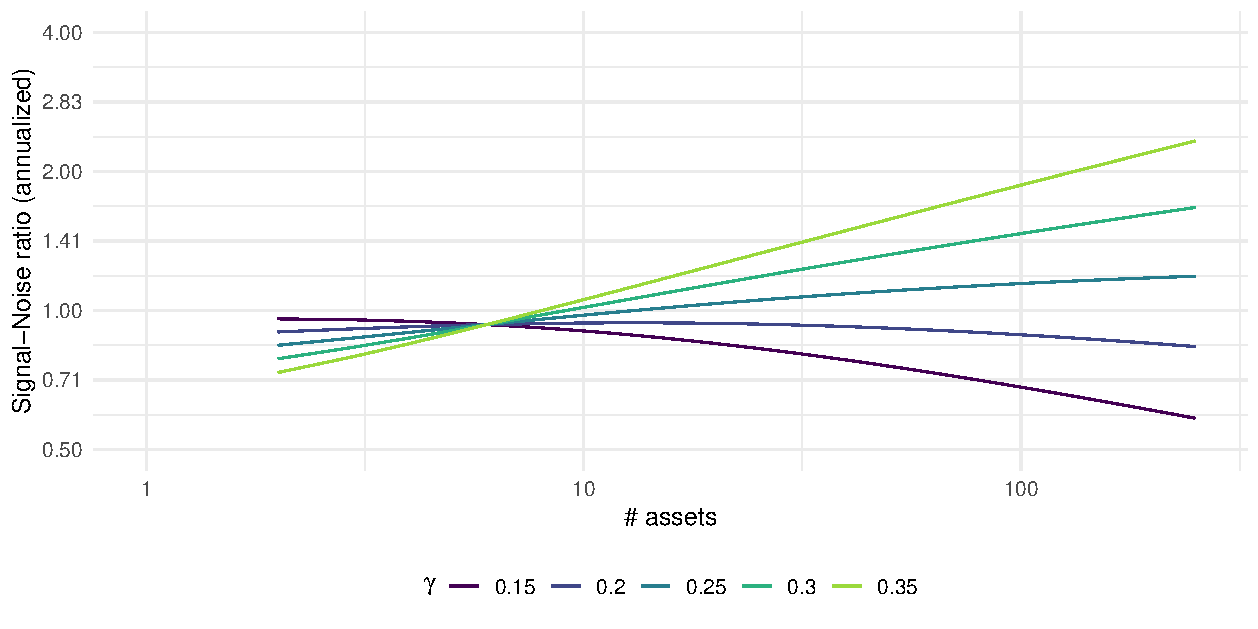
\includegraphics[width=0.99\textwidth,height=0.495\textwidth]{figure/qboundgrow_bound-1} \caption[The upper bound of \theoremref{qual_bound} is plotted versus \nlatf for different scaling laws.]{The upper bound of \theoremref{qual_bound} is plotted versus \nlatf for different scaling laws.}\label{fig:grow_bound}
\end{figure}

\end{knitrout}

The decreasing upper bound with respect to growing universe size
is illustrated in \figref{grow_bound}. Under the assumption
$\psnropt = \psnr[0]\nlatf^{\gamma}$, the upper bound
of \theoremref{qual_bound} is plotted versus \nlatf for 
different values of $\gamma$. 
The value of
$\psnr[0]$ is set so that 
$\psnropt=1.25\yrtomhalf$ when 
$\nlatf=6$.
For $\gamma < \oneby{4}$, one sees a local maximum in 
the upper bound as \nlatf increases, a behavior not seen for
$\gamma > \oneby{4}$, where the bound on \txtQual
grows with \nlatf. 


%$\psnropt$ and the $0.25, 0.50,$ and $0.75$ quantiles of
%$\psnropt\pql{\sportwfnc{\mreti}}$, under 
%\apxref{qual_dist}, are plotted versus \nlatf.
%The panels represent $\gamma$ values of
%$sort(pgammas)[1:(length(pgammas)-1)],$ and 
%$sort(pgammas)[length(pgammas)]$.
%The value of
%$\psnr[0]$ is set so that 
%$\psnropt=sqrt(ope)*zeta.s\yrtomhalf$ when 
%$\nlatf=n.stok$.
%For $\gamma < 0.25$, one sees a local maximum in 
%achieved \txtSR as \nlatf increases, a behavior not seen for
%$\gamma > 0.25$, where achieved \txtSR grows with \nlatf. 
%For the case of `slow growth' of \psnropt, the diversification 
%benefit is not seen by the sample \txtMP, rather its practical
%utility \emph{decreases} because the haircut outpaces the growth
%of \psnropt. As a practical matter, this may explain why the
%\txtMP is typically applied to small asset universes.



This relationship between \txtQual and \nlatf for different
values of $\gamma$ appears not just in the upper bound of
\theoremref{qual_bound}, but apparently also for most quantiles
of the distribution given by \apxref{qual_dist}, as
%This loss in value with respect to growing universe size is
illustrated in \figref{grow_sqrt}. Again assuming
$\psnropt = \psnr[0]\nlatf^{\gamma}$, lines of 
$\psnropt$ and the $0.25, 0.50,$ and $0.75$ quantiles of
$\psnropt\pql{\sportwfnc{\mreti}}$, under 
\apxref{qual_dist}, are plotted versus \nlatf.
The panels represent $\gamma$ values of
$0.15, 0.2, 0.25, 0.3,$ and 
$0.35$.
Again, the value of
$\psnr[0]$ is set so that 
$\psnropt=1.25\yrtomhalf$ when 
$\nlatf=6$.
For $\gamma < \oneby{4}$, one sees a local maximum in 
\txtQual as \nlatf increases, a behavior not seen for
$\gamma > \oneby{4}$, where quantiles of \txtQual grow with \nlatf. 
For the case of `slow growth' of \psnropt, the diversification 
benefit is not seen by the sample \txtMP, rather its practical
utility \emph{decreases} because the estimation error 
outpaces the growth of \psnropt. 

%Via the equivalence in \eqnref{sufficient_growth}, for the 
%bound \qbnd to be growing with respect to \nlatf, it suffices
%to establish that 
%$\half \le \wrapParens{\nlatf-1}\dbyd{\log\psnrsqopt}{\nlatf}$.
%From \eqnref{capm_zetas}, we have
%\begin{equation*}
%\begin{split}
%\half\dbyd{\log\psnrsqopt}{\nlatf} 
%&= 
%\frac{\trAB{\vect{\alpha}}{\dbyd{\vect{\alpha}}{\nlatf}} + 
%\wrapParens{\frac{\sigma_m}{\sigma}}^2 \wrapBracks{
 %\trAB{\vect{\beta}}{\dbyd{\vect{\beta}}{\nlatf}}\gram{\vect{\alpha}}
%+ \trAB{\vect{\alpha}}{\dbyd{\vect{\alpha}}{\nlatf}}\gram{\vect{\beta}}
%- \trAB{\vect{\alpha}}{\vect{\beta}}\wrapParens{
  %\trAB{\vect{\alpha}}{\dbyd{\vect{\beta}}{\nlatf}} + 
  %\trAB{\vect{\beta}}{\dbyd{\vect{\alpha}}{\nlatf}}}}}{%
%\gram{\vect{\alpha}} +
%\wrapParens{\frac{\sigma_m}{\sigma}}^2 \wrapBracks{%
%\gram{\vect{\beta}}\gram{\vect{\alpha}} -
%\wrapParens{\trAB{\vect{\alpha}}{\vect{\beta}}}^2}}
%+ \frac{\sigma_m^2 \trAB{\vect{\beta}}{\dbyd{\vect{\beta}}{\nlatf}}}{%
%\sigma^2 + \sigma_m^2\gram{\vect{\beta}}}.
%\end{split}
%\end{equation*}
%2FIX: where you going with this?
%These plots are built using \apxref{hcut_apx} ...

\subsection{Diversification under CAPM}%FOLDUP

It is not clear how \psnropt `should' scale with \nlatf. It is
easy to construct a model under which \psnropt scales as
$\nlatf^{\half}$: assume all assets have independent returns with
the same \txtSNR. It is also easy to accidentally construct 
a model under which \psnropt ultimately scales 
as $\nlatf^{\epsilon}$ for small $\epsilon$, as done here.
Suppose the \kth{i} asset has expected return
$\alpha_i$, exposure $\beta_i$ to `the market', and volatility
$\sigma$. Assume the market return is zero mean with volatility
$\sigma_m$. Then the squared \txtSNR is
\begin{align}
\nonumber
\psnrsqopt 
&= 
\frac{\gram{\vect{\alpha}} +
\wrapParens{\frac{\sigma_m}{\sigma}}^2 \wrapBracks{%
\gram{\vect{\beta}}\gram{\vect{\alpha}} -
\wrapParens{\trAB{\vect{\alpha}}{\vect{\beta}}}^2}}{\sigma^2 +
\sigma_m^2\gram{\vect{\beta}}},&\\
&= 
\frac{\gram{\vect{\alpha}}}{\sigma^2}
\frac{\sigma^2 + \sigma_m^2 \gram{\vect{\beta}} \fsin[2]{\psi}}{%
\sigma^2 + \sigma_m^2\gram{\vect{\beta}}},&
\label{eqn:capm_zetas}
\end{align}
where $\psi$ is the angle between the vectors \vect{\alpha}
and \vect{\beta}.
Depending on how the sine of $\psi$ grows with universe size, 
one observes different scaling of \psnropt with respect to \nlatf. When
the assets all have the same alpha and beta, \ie
$\vect{\alpha} = \alpha\vone$ and $\vect{\beta} = \beta\vone$,
the sine is identically zero, and 
$\psnropt = \sqrt{\fraccp{\nlatf\alpha^2}{\sigma^2 + \nlatf\sigma_m^2\beta^2}}
< \alpha\beta^{-1}\sigma_m^{-1}$. Thus 
\psnropt asymptotically scales slower than $\nlatf^{\epsilon}$
for all $\epsilon > 0$.

On the other hand, when the sine is
one, \ie when \vect{\alpha} is orthogonal to \vect{\beta},
$\psnropt = \sqrt{\gram{\vect{\alpha}}} \sigma^{-1}$, which
grows however the assets are ordered, presumably on the
order of $\nlatf^{\half}$. Thus under a CAPM model, the
growth of \psnropt depends on the `alignment' of the
vectors \vect{\alpha} and \vect{\beta}.
%UNFOLD

%UNFOLD

%%%%%%%%%%%%%%%%%%%%%%%%%%%%%%%%%%%%%%%%%%%%%%%%%%%%%%%%%%%%%%%%%%%%%%%%
\section{Generalizations}%FOLDUP

\label{sec:generalizations}

\theoremref{qual_bound} is somewhat lacking because it ignores conditioning
information which may affect the distribution of future returns, and which
may inform the portfolio manager. Few active managers, it is presumed,
are holding the unconditional \txtMP based on in-sample data. What is sought
is a more general theorem that allows more elaborate models of returns,
and more elaborate, parametrized, trading schemes, with \psnropt redefined 
as the maximal portfolio \txtQual over the trading schemes, and \nlatf
redefined as the `degrees of freedom', perhaps the rank of some derivative
at the optimal parameter, say. Towards that goal, a few generalizations can
easily be made.

\subsection{Conditional portfolio \txtQual}%FOLDUP
\label{subsec:cond_portfolio_qual}

The model of stationary mean returns is generalized by one where
the expected return of the assets is linear in some state
variables, or `features', \vfact[i], observed prior to the investment
decision.  \cite{pav_the_book,connor1997,herold2004TAA} That
is, one observes the \nfac-vector $\vfact[i]$ at some time prior to 
when the investment decision is required to capture \vreti[i+1]. 
The general model is now
\begin{align}
\label{eqn:cond_model_IV}
\Econd{\vreti[i+1]}{\vfact[i]} &=
\pRegco \vfact[i], &
\Varcond{\vreti[i+1]}{\vfact[i]} &=
\pvsig,
\end{align}
where \pRegco is some \bby{\nlatf}{\nfac} matrix. 

Here we bound the \txtQual of portfolios which are
linear in the features \vfact[i]. That is, the portfolio
manager allocates their assets proportional to
$\sportW\vfact[i]$ for some matrix $\sportW$.

Using the law of iterated expectations, the unconditional
expected value of the returns of the portfolio is
\begin{equation*}
\E{\Econd{\trAB{\wrapParens{\sportW\vfact[i]}}{\vreti[i+1]}}{\vfact[i]}}
= \trace{\tr{\sportW}\pRegco\E{\ogram{\vfact[i]}}}
= \trace{\tr{\sportW}\pRegco\pfacsig},
\end{equation*}
by definition of \pfacsig as the second moment of \vfact[i].

Unfortunately the unconditional variance will, in general,
involve a term quadratic in the expectation. However, it
can easily be shown that the unconditional \emph{expected} 
variance of the portfolio's returns is
\begin{equation*}
\E{\qform{\pvsig}{\wrapParens{\sportW\vfact[i]}}} =
\trace{\qform{\pvsig}{\sportW}\pfacsig}.
\end{equation*}
We can then redefine\footnote{If an analysis of the conditional expected
return divided by risk is required, it is possible one could define
\pQl{\cdot} as the expected return divided by square root of the unconditional
second moment. The \txtQual would then be $\ftan{\farcsin{\pQl{\cdot}}}$.
One could possibly find a \txtCR bound on the expected value of this \pQl{\cdot}.
This `Pillai-Bartlett' form of \pQl{\cdot} is likely unrequired for low frequency
settings.} the \txtQual of the portfolio as the
unconditional mean divided by the unconditional expected risk:
\begin{equation}
\pQl{\sportW}\defeq\frac{\trace{\tr{\sportW}\pRegco\pfacsig}}{%
\sqrt{\trace{\qform{\pvsig}{\sportW}\pfacsig}}}.
\end{equation}
When \vfact[i] is a deterministic scalar constant, 
this coincides with the `usual' definition of \txtQual as being 
like a \txtSR. However, except possibly for an intercept term, one
expects \vfact[i] to be random, or at least out of the control of
the portfolio manager.

Once again, a risk transform can be injected to express
portfolio optimization as an estimation problem on a sphere:
\begin{equation}
\begin{split}
\pQl{\sportW}
&=\frac{\trace{\trAB{%
\wrapParens{\trchol{\pvsig}\sportW\chol{\pfacsig}}}{%
\wrapParens{\ichol{\pvsig}\pRegco\chol{\pfacsig}}}{%
}}}{%
\sqrt{\trace{
\gram{\wrapParens{\trchol{\pvsig}\sportW\chol{\pfacsig}}}}}},\\
&=
\frac{\trAB{\fvec{\trchol{\pvsig}\sportW\chol{\pfacsig}}}{%
\fvec{\ichol{\pvsig}\pRegco\chol{\pfacsig}}}}{%
\sqrt{\gram{\fvec{\trchol{\pvsig}\sportW\chol{\pfacsig}}}}}.
\end{split}
\end{equation}
This function is maximized by taking
\begin{equation}
\sportW = \pportWopt \defeq \minv{\pvsig}{\pRegco},
\end{equation}
which has \txtQual
\begin{equation}
\psnropt\defeq\pQl{\pportWopt} =
\sqrt{\trace{\qiform{\pvsig}{\pRegco}\pfacsig}}.
\end{equation}
The square of this quantity, \psnrsqopt, 
is the `population analogue' of the Hotelling-Lawley trace. \cite{Rencher2002,Muller1984143}

Again we can write
\begin{equation*}
\frac{\pQl{\sportW}}{\psnropt} = 
\trAB{\fnorm{\fvec{\trchol{\pvsig}\sportW\chol{\pfacsig}}}}{%
\fnorm{\fvec{\ichol{\pvsig}\pRegco\chol{\pfacsig}}}}.
\end{equation*}
Thus finding a `good' \sportW becomes an estimation problem on the
sphere \sphere{\nfac\nlatf - 1}. An analogue
to \theoremref{qual_bound} can be proved with $\nfac\nlatf$ replacing
$\nlatf$, by assuming a particular form to the likelihood. We must
generalize the assumption of Directional Independence, after which
the theorem proceeds easily.

\begin{assumption}[Conditional Directional Independence]%FOLDUP
Assume that
\begin{equation}
\label{eqn:sane_estimator_cond}
\E{\fnorm{\fvec{\trchol{\pvsig}\sportWfnc{\mreti,\mfact}}}} = 
\cfnc{\psnrsqopt} \fnorm{\fvec{\trchol{\pvsig}\pportWopt\chol{\pfacsig}}}
+ \Bterm,
\end{equation}
where \Bterm is the bias term, orthogonal to 
\fnorm{\fvec{\trchol{\pvsig}\pportWopt\chol{\pfacsig}}}.
\end{assumption}%UNFOLD

\begin{theorem}%FOLDUP
\label{theorem:qual_bound_two}
Let one element of \vfact[i] be a deterministic $1$. Suppose the
vector of the remaining $\nfac-1$ elements of \vfact[i] stacked 
on top of \vreti[i+1] are multivariate Gaussian.  Let \mreti, 
\mfact be \bby{\ssiz}{\nlatf} and \bby{\ssiz}{\nfac} matrices
of \iid observations of the features and returns.
Let \sportWfnc{\mreti,\mfact} be an estimator 
%based on 
%\ssiz \iid observations of multivariate Gaussian returns, \mreti, 
%and multivariate Gaussian features, \mfact, with one column of \mfact
%an intercept term, 
satisfying the assumptions of
Conditional Directional Independence and Residual Independence. Then
\begin{equation}
\E{\pQl{\sportWfnc{\mreti,\mfact}}} 
\le \frac{\sqrt{\ssiz}\psnrsqopt}{\sqrt{\nfac\nlatf - 1 + \ssiz\psnrsqopt}}.
\end{equation}
\end{theorem}%UNFOLD
\begin{proof}%FOLDUP

We can proceed as in \secref{portfolio_qual}. Let \mreti be the 
\bby{\ssiz}{\nlatf} matrix of portfolio returns, and let 
\mfact be the corresponding \bby{\ssiz}{\nfac} matrix of features.
View the portfolio coefficient \sportW as an estimator, a function of
the random data, \ie \sportWfnc{\mreti,\mfact}.
%Assume
%Directional Independence, with \eqnref{sane_estimator}
%becoming
%\begin{equation}
%\E{\fnorm{\trchol{\pvsig}\sportWfnc{\mreti,\mfact}}} = 
%\cfnc{\psnrsqopt} \fnorm{\trchol{\pvsig}\pportWopt\chol{\pfacsig}}
%+ \Bterm.
%\end{equation}
Define
\begin{equation}
\prskMtx\defeq{\ichol{\pvsig}\pRegco\chol{\pfacsig}}.
\end{equation}
Then 
\begin{equation*}
\psnrsqopt = \trace{\gramprskMtx}.
\end{equation*}

We get, analogously to \eqnref{crb_one},
\begin{equation}
\oneby{\ssiz}\trace{\qoform{\iFishI[\fvec{\prskMtx}]}{\Drv}}
\le 1 - \csqfnc{\trace{\gramprskMtx}},
\end{equation}
where
\begin{equation}
\Drv\defeq
{\dbyd{\cfnc{\trace{\gramprskMtx}}\frac{\prskMtx}{\sqrt{\trace{\gramprskMtx}}}}{\fvec{\prskMtx}}}.
\end{equation}

Without loss of generality, we assume it is the first element
of \vfact[i] that is a deterministic $1$. Then, the log likelihood of 
the vector of $\vfact[i]$ stacked on top of $\vreti[i+1]$
is: \cite{pav2013markowitz}
\begin{equation}
\label{eqn:cond_llik_one}
\log \FOOlik{}{\pvsm}{\twobyone{\vfact[i]}{\vreti[i+1]}} = 
  c_{\nfac+\nlatf} 
- \half \logdet{\pvsm} 
- \half \trace{\minv{\pvsm}\ogram{\twobyone{\vfact[i]}{\vreti[i+1]}}},
\end{equation}
where \pvsm is the second moment matrix:
\begin{equation}
\pvsm \defeq \E{\ogram{\twobyone{\vfact[i]}{\vreti[i+1]}}}
= \twobytwo{\pfacsig}{\pfacsig\tr{\pRegco}}{\pRegco\pfacsig}{\pvsig +
\qoform{\pfacsig}{\pRegco}}.
%\qoform{\pfaccov}{\pRegco}}}.
\end{equation}
The inverse of \pvsm has the following, somewhat surprising, form \cite{pav2013markowitz}:
\begin{equation}
\minv{\pvsm} 
= \twobytwo{\minv{\pfacsig} +
\qiform{\pvsig}{\pRegco}}{-\tr{\pRegco}\minv{\pvsig}}{-\minv{\pvsig}\pRegco}{\minv{\pvsig}}.
\end{equation}
A square root of this matrix (a Cholesky factor, up to permutation)
is:
\begin{equation}
\begin{split}
\minv{\pvsm} &=
\ogram{%
\twobytwo{\ichol{\pfacsig}}{-\tr{\pRegco}\ichol{\pvsig}}{\mzero}{\ichol{\pvsig}}
},\\
&= \twobytwo{\ichol{\pfacsig}}{\mzero}{\mzero}{\eye}
\ogram{%
\twobytwo{\eye}{-\prskMtxU{\trsym}}{\mzero}{\ichol{\pvsig}}}
\twobytwo{\trichol{\pfacsig}}{\mzero}{\mzero}{\eye}.
\end{split}
\end{equation}

By the block determinant formula, 
\begin{equation}
\det{\pvsm} 
= \det{\pfacsig}\det{\pvsig + \qoform{\pfacsig}{\pRegco} -
\pRegco\pfacsig\minv{\pfacsig}\pfacsig\tr{\pRegco}}
= \det{\pfacsig}\det{\pvsig}.
\end{equation}
Thus, conditional on \pfacsig and \pvsig, the negative log likelihood
takes the form:
\begin{multline}
\label{eqn:cond_llik_two}
- \log \FOOlik{}{\prskMtx, \pfacsig, \pvsig}{\twobyone{\vfact[i]}{\vreti[i+1]}} = 
- c_{\nfac+\nlatf}
+ \half \logdet{\pfacsig} 
+ \half \logdet{\pvsig}\\
+ \half \trace{
\ogram{%
\twobytwo{\eye}{-\prskMtxU{\trsym}}{\mzero}{\ichol{\pvsig}}}
\ogram{\twobyone{\trichol{\pfacsig}\vfact[i]}{\vreti[i+1]}}}.
\end{multline}
Sweeping the nuisance parameter terms into the constant, as well
as terms in the trace which are not quadratic in \prskMtx, we
have 
\begin{align}
\label{eqn:cond_llik_three}
- \log \FOOlik{}{\prskMtx, \pfacsig, \pvsig}{\twobyone{\vfact[i]}{\vreti[i+1]}}
&= - c'
+ \half \trace{\gramprskMtx 
\ogram{\wrapParens{\trichol{\pfacsig}\vfact[i]}}},&\\
&= - c'
+ \half
\tr{\fvec{\prskMtx}}\fvec{\prskMtx\trichol{\pfacsig}\ogram{\vfact[i]}\ichol{\pfacsig}}.&\\
&= - c'
+ \half
\tr{\fvec{\prskMtx}}\wrapParens{%
\wrapBracks{\trichol{\pfacsig}\ogram{\vfact[i]}\ichol{\pfacsig}}
 \kron \eye}\fvec{\prskMtx}.&
\end{align}
The Fisher Information, then, is
\begin{equation}
\FishI[\fvec{\prskMtx}] =
\E{\wrapParens{%
\wrapBracks{\trichol{\pfacsig}\ogram{\vfact[i]}\ichol{\pfacsig}}
 \kron \eye}} = \eye[\nfac\nlatf].
\end{equation}

The remainder of the proof proceeds exactly as in 
\secref{portfolio_qual}. 
\end{proof}%UNFOLD

%\begin{theorem}
%\label{theorem:qual_bound_two}
%Let \sportWfnc{\mreti,\mfact} be an estimator based on 
%\ssiz \iid observations of multivariate Gaussian returns, \mreti, 
%and multivariate Gaussian features, \mfact, with one column of \mfact
%an intercept term, satisfying the assumptions of
%directional independence and residual independence. Then
%\begin{equation}
%\E{\pQl{\sportWfnc{\mreti,\mfact}}} 
%\le \frac{\sqrt{\ssiz}\psnrsqopt}{\sqrt{\nlatf\nfac - 1 + \ssiz\psnrsqopt}}.
%\end{equation}
%\end{theorem}

%&= \E{\Cmat\scoro{\prskvec}{\FOOlik{}{\prskvec}{\mreti}}

%\begin{equation}
%\begin{split}
%\vfact[i] &\sim \normlaw{\pfacmu, \pfaccov},\\
%\condtwo{\vreti[i+1]}{\vfact[i]} &\sim \normlaw{\pRegco\vfact[i], \pvsig}.
%\end{split}
%\end{equation}
%Together the unconditional distribution is
%\begin{equation}
%\twobyone{\vfact[i]}{\vreti[i+1]} \sim
%\normlaw{\twobyone{\pfacmu}{\pRegco\pfacmu}, 
%\twobytwo{\pfaccov}{\pfaccov\tr{\pRegco}}{\pRegco\pfaccov}{\pvsig +
%\qoform{\pfaccov}{\pRegco}}}.
%\end{equation}




%In this model, the `Markowitz Coefficient' 
%$\minvAB{\pvsig}{\pRegco}$, generalizes the \txtMP as
%the coefficient of the optimal portfolio which is linear in \vfact,
%under some objective. \cite{pav2013markowitz} How should we define
%the \txtQual of the Markowitz Coefficient, and can we prove
%an analogue of \theoremref{qual_bound}?
%UNFOLD

\subsection{Subspace constraints}%FOLDUP

Consider, now, the case of conditional expectation, as presented in
\subsecref{cond_portfolio_qual}, but where the portfolio is 
constrained to be in some lower dimensional subspace. That is, by design, 
\begin{equation}
\zerJc \sportWfnc{\mreti,\mfact} = \vzero,
\end{equation}
where $\zerJc$ is a \bby{\wrapParens{\nlatf - \nlatfzer}}{\nlatf}
matrix of rank $\nlatf - \nlatfzer$, that is chosen independently
of the observations of \mreti and \mfact.
Let the rows of \zerJ span the null space of the rows of
\zerJc; that is, $\zerJc \tr{\zerJ} = \mzero$, and $\ogram{\zerJ} = \eye$.

We can simply use the results of \subsecref{cond_portfolio_qual}, but
replacing the assets with the \nlatfzer assets spanned by the rows of
\zerJ. That is, we can replace the \vreti[i+1] with $\zerJ\vreti[i+1]$,
and replace \sportWfnc{\mreti,\mfact} with
$\tr{\zerJ}\minv{\wrapParens{\ogram{\zerJ}}}\sportWfnc{\mreti,\mfact}$
to arrive at the following analogue of \theoremref{qual_bound_two}:

\begin{theorem}%FOLDUP
\label{theorem:qual_bound_three}
Let one element of \vfact[i] be a deterministic $1$. Suppose the
vector of the remaining $\nfac-1$ elements of \vfact[i] stacked 
on top of \vreti[i+1] are multivariate Gaussian.  Let \mreti, 
\mfact be \bby{\ssiz}{\nlatf} and \bby{\ssiz}{\nfac} matrices
of \iid observations of the features and returns.
Let \sportWfnc{\mreti,\mfact} be an estimator 
%based on 
%\ssiz \iid observations of multivariate Gaussian returns, \mreti, 
%and multivariate Gaussian features, \mfact, with one column of \mfact
%an intercept term, 
satisfying the assumptions of
directional independence and residual independence, with the constraint
\begin{equation}
\zerJc \sportWfnc{\mreti,\mfact} = \vzero,
\end{equation}
for \bby{\wrapParens{\nlatf - \nlatfzer}}{\nlatf} matrix \zerJc, which
is chosen independently of the observed \mreti and \mfact. 
Let the rows of \zerJ span the null space of the rows of
\zerJc. 

Then
\begin{equation}
\E{\pQl{\sportWfnc{\mreti,\mfact}}} 
\le \frac{\sqrt{\ssiz}\psnrsqoptG{\zerJ}}{\sqrt{\nfac\nlatfzer - 1 +
\ssiz\psnrsqoptG{\zerJ}}},
\end{equation}
where 
\begin{equation*}
\psnrsqoptG{\zerJ}\defeq 
\trace{\qform{\wrapProj{\pvsig}{\zerJ}}{\pRegco}\pfacsig}.
\end{equation*}
\end{theorem}%UNFOLD
%UNFOLD

\subsection{Hedging constraints}%FOLDUP

Consider, now, the case where one seeks a portfolio whose returns are
independent, in the probabilistic sense, of the returns of some 
traded instruments in the investment universe. 
Independence is a difficult property to
check or enforce; however, independence implies zero covariation, which
can be easily formulated and checked. 

Since the portfolio estimator may not deliver a perfectly
hedged portolio due to misestimation of the covariance matrix, we
will, with perfect knowledge of \pvsig, consider the \txtQual of the 
hedged part of the portfolio. The hedged
part is defined in terms of a risk projection. 
If \sportw[1] is a feasible portfolio based on the sample,
then the hedged version of this portfolio is the solution to the
optimization problem
\begin{equation}
\min_{\sportw : \hejG\pvsig\sportw = \vzero} \VAR{\trAB{\wrapParens{\sportw -
\sportw[1]}}{\vreti[i+1]}},
\end{equation}
where $\hejG$ is a \bby{\nlatfhej}{\nlatf} matrix of 
rank \nlatfhej, the rows of which we wish to `hedge out.'

Using the Lagrange multiplier technique, this can easily be found to
be solved by 
\begin{equation}
\sportw = \sportw[1] - \wrapProj{\pvsig}{\hejG}\pvsig\sportw[1].
\end{equation}
Thus we will consider the \txtQual of the portfolio estimator
\begin{equation*}
\wrapParens{\eye[\nlatf] - \wrapProj{\pvsig}{\hejG}\pvsig}\sportWfnc{\mreti,\mfact}.
\end{equation*}
Note, however, that the row rank of
$\wrapParens{\eye[\nlatf] - \wrapProj{\pvsig}{\hejG}\pvsig}$ 
is $\nlatf - \nlatfhej$.  Thus hedging is an instance of a subspace
constraint and we can apply \theoremref{qual_bound_three} outright.

\begin{theorem}%FOLDUP
\label{theorem:qual_bound_four}
Let one element of \vfact[i] be a deterministic $1$. Suppose the
vector of the remaining $\nfac-1$ elements of \vfact[i] stacked 
on top of \vreti[i+1] are multivariate Gaussian.  Let \mreti, 
\mfact be \bby{\ssiz}{\nlatf} and \bby{\ssiz}{\nfac} matrices
of \iid observations of the features and returns.
Let \sportWfnc{\mreti,\mfact} be an estimator 
%based on 
%\ssiz \iid observations of multivariate Gaussian returns, \mreti, 
%and multivariate Gaussian features, \mfact, with one column of \mfact
%an intercept term, 
satisfying the assumptions of
directional independence and residual independence. 
Let \bby{\nlatfhej}{\nlatf} matrix \hejG be chosen
independently of \mreti and \mfact. 

%2FIX: redefine Deltapsnr to not be confusing.
Define 
\begin{equation}
\Delpsnrsqopt{\eye,\hejG}
\defeq
\trace{\qiform{\svsig}{\pRegco}\pfacsig} - 
\trace{\qform{\wrapProj{\pvsig}{\hejG}}{\pRegco}\pfacsig}.
\end{equation}

Then
\begin{equation}
\E{\pQl{%
\wrapBracks{\eye[\nlatf] - \wrapProj{\pvsig}{\hejG}\pvsig}\sportWfnc{\mreti,\mfact}}} 
\le \frac{\sqrt{\ssiz}\Delpsnrsqopt{\eye,\hejG}}{\sqrt{\nfac\wrapParens{\nlatf -
\nlatfhej} - 1 + \ssiz\Delpsnrsqopt{\eye,\hejG}}}.
\end{equation}
\end{theorem}%UNFOLD

%UNFOLD

%UNFOLD

%%%%%%%%%%%%%%%%%%%%%%%%%%%%%%%%%%%%%%%%%%%%%%%%%%%%%%%%%%%%%%%%%%%%%%%%
\section{Examples}%FOLDUP

\subsection{The equal weight puzzle}%FOLDUP


\theoremref{qual_bound} can help us make sense of puzzling findings
in the literature. For example, in the ``$1/N$'' paper, DeMiguel \etal
find that the equal-weighting portfolio outperforms, in terms of out-of-sample
\txtSR (and other measures), the \txtMP and numerous other portfolio
estimators.  \cite{demiguel2009optimal}
This finding is supported on a number of real world data
sets, and a few synthetic ones. One data set used was the returns of
the 10 industry portfolios and the US equity market portfolio, computed
by Ken French. 
% 2FIX: add citation to data.

The monthly returns, from 1927-01-01 to 
2020-12-01, for these 10 
assets were downloaded
from Kenneth French's data library.  \cite{French10Port}
%from \emph{Quandl}.  \cite{Quandl}
The \txtSR of the equal weighted portfolio on the %10
assets, over the 1128 months, is around 
$0.67\yrtomhalf$. The \txtSR of the sample \txtMP over
the 10 assets over the same period is around
$0.86\yrtomhalf$.  
Now consider a portfolio estimator
given 5 years of observations, as in 
DeMiguel \etal \cite{demiguel2009optimal}, assuming 
$\psnropt=0.86\yrtomhalf$.
The bound on expected value of \pql{\sportwfnc{\mreti}} from \theoremref{qual_bound} is only $0.46\yrtomhalf$.  
%Under \apxref{qual_dist}, the probability that \pql{\sportwfnc{\mreti}} exceeds $sr1$sr\yrtomhalf$ in this case is only $dfp$. 
It is not surprising that DeMiguel \etal drew
the conclusions they did, nor that they would be refuted
by looking at a longer sample, as by Kritzman \etal \cite{defoopt2010}



One could also use \theoremref{qual_bound_four} here. However,
the upper bound of that theorem is non-negative, and zero only
if the quantity \Delpsnrsqopt{\eye,\hejG} is zero.  This is a
statement regarding unknown population parameters, but we can
perform inference on this quantity. For example, based on the
1128 months of data on these 
10, the 95\% confidence interval on
\Delpsnrsqopt{\eye,\hejG}, where \hejG is the \bby{1}{10}
matrix of all ones, is
$\asrowvec{0.04, 0.45}\yrto{-1}$, under the assumption of
Gaussian returns.  

%One could view the touted superiority of the equal weight portfolio
%over \eg the \txtMP as a veiled claim that there is a single
%discount factor that rules all asset returns. As stated, this claim
%is clearly absurd, since \eg an equal weight portfolio on both pairs
%of leveraged ETFs is clearly inferior to a portfolio equal weight \emph{short}
%both pairs.  \cite{zhang2010path}

%This highlights
%the fact that the putative superiority of the equal weight portfolio
%may be based on two due less to deficiencies in \eg the \txtMP, and more to
%the 

%The analysis presented here is likely to be optimistic when one
%considers the \emph{spanning} aspect of this problem.  
%\cite{giri1964likelihood,HKspan1987,KanZhou2012} That is, the
%total effect size beyond the equal weighting subspace may be
%very small. A `proper' analysis would take into account the
%difference in effect sizes and differences in universe size. 
%However, the spanning analogue of \theoremref{qual_bound}
%has not yet been established.

%% 2FIX: talk about the spanning statistics here. is there
%% any effect to exploit?
%The result is dKRS or
%dUNB or
%dMLE.
%the upper bound is asqb.
%Show it as:
%dsr2
%or cis: myci.

%UNFOLD

\subsection{Empirical diversification in the S\&P 100}%FOLDUP



To check how \psnropt \emph{might} scale with \nlatf, the weekly
log returns of the adjusted close prices of the stocks in the 
S\&P 100 Index, as of March 21, 2014, were downloaded 
from \emph{Quandl}.  \cite{Quandl} 
Adjustments for splits and
dividends were made in some unspecified way by the upstream source
of the data, Yahoo Finance. Stocks without a full 5 years of history
were discarded, leaving 96 stocks. 
Note that selection based on membership in the index at the end of the 
period adds no small amount of selection bias, which we shall ignore 
here.

Based on the weekly returns from 2009-03-27 to 2014-04-04,
estimates of \psnropt were computed, using the `KRS' estimator.
\cite{kubokawa1993estimation,pav_the_book} 
This was performed on the first \nlatf assets, with \nlatf ranging from 
$1$ to $96$.  The estimate of \psnropt versus \nlatf
is plotted in \figref{sp100_grow}, with assets added in alphabetical order.
Because Apple appears at the beginning of this list, it appears that
\psnropt starts reasonably large, but then actually \emph{decreases}
when adding assets. This is an artifact of the estimator, since the true
\psnropt can only increase when adding assets. 

\begin{knitrout}\small
\definecolor{shadecolor}{rgb}{0.969, 0.969, 0.969}\color{fgcolor}\begin{figure}[h]
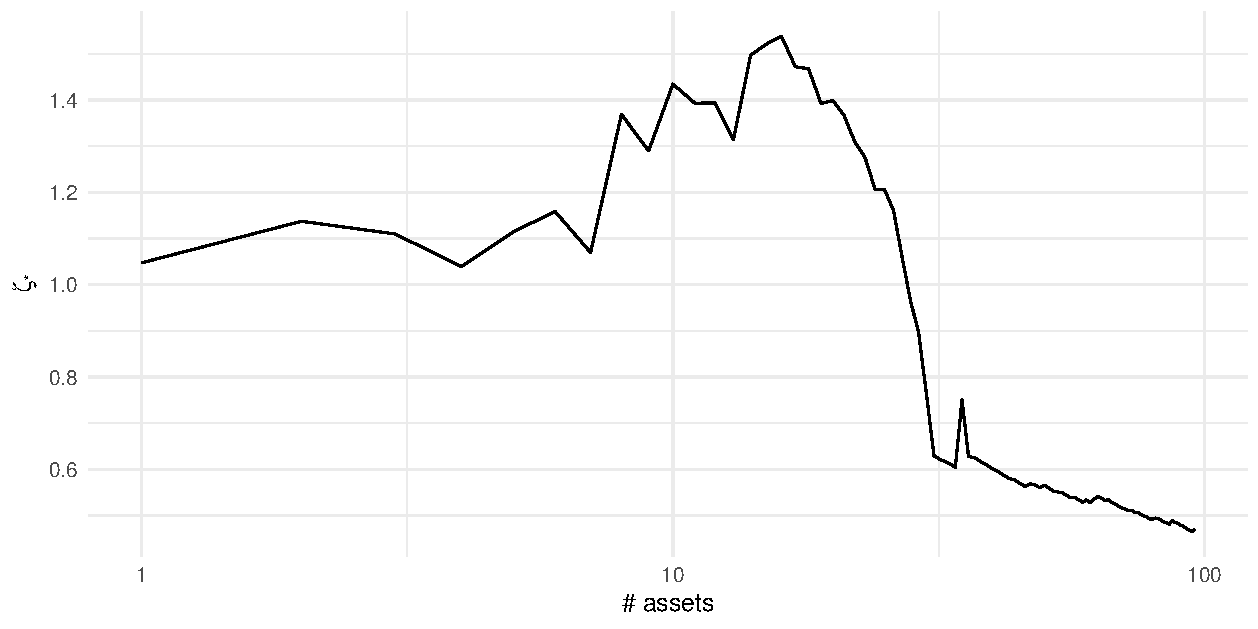
\includegraphics[width=0.99\textwidth,height=0.495\textwidth]{figure/qboundsp100_grow-1} \caption[Growth of estimated \psnropt versus \nlatf for the S\&P 100 Index names, in alphabetical order, showing the `Apple effect.']{Growth of estimated \psnropt versus \nlatf for the S\&P 100 Index names, in alphabetical order, showing the `Apple effect.'}\label{fig:sp100_grow}
\end{figure}

\end{knitrout}

%<<'sp100_mid',eval=TRUE,cache=FALSE,fig.width=5.75,fig.height=3.75,dpi=450,fig.cap=paste0("Growth of estimated \\psnropt versus \\nlatf for the S\\&P 100 Index names."),eval.after='fig.cap'>>= 

%foo.df <- data.frame(df=(1:length(KRSs)),KRS=KRSs,
		%MLE=MLEs,meanKRS=rowMeans(buncho.KRSs))

%require(ggplot2)
%ph <- ggplot(data=foo.df,aes(x=df,y=meanKRS))
%ph <- ph + geom_line()
%ph <- ph + labs(x="# assets",
								%y=expression(zeta["*"]))
%ph <- ph + scale_x_log10()
%ph <- ph + scale_y_log10()
%print(ph)

%@

Since the ordering of assets here is arbitrary, the experiment was repeated
1000 times, with the stocks randomly permuted, and 
\psnropt estimated as a function of \nlatf. Boxplots, over the
1000 simulations, of the KRS statistic versus
\nlatf are given in \figref{sp100_box}. There is effectively no 
diversification benefit observed here beyond the mean effect, which is
equivalent to holding an equal weight portfolio. Given the 
conditions under which \txtQual grows with \nlatf outlined in 
\secref{diversification}, one expects poor performance of 
directionally independent portfolio estimators
over even a small subset of the S\&P 100.

\begin{knitrout}\small
\definecolor{shadecolor}{rgb}{0.969, 0.969, 0.969}\color{fgcolor}\begin{figure}[h]
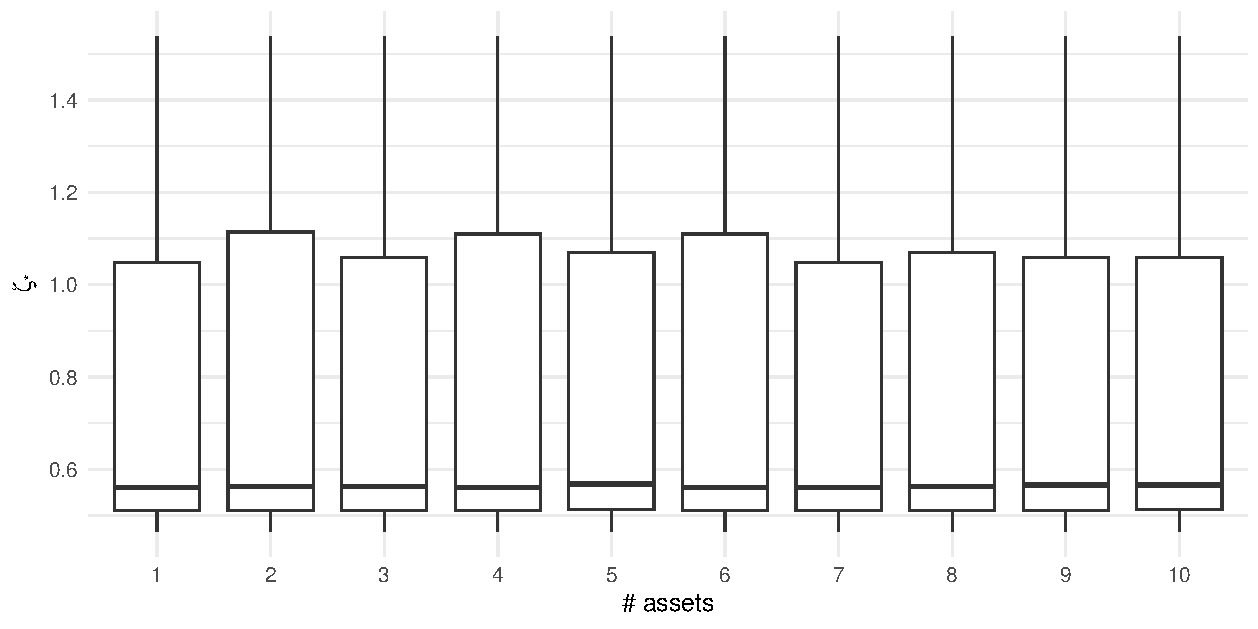
\includegraphics[width=0.99\textwidth,height=0.495\textwidth]{figure/qboundsp100_box-1} \caption[Growth of estimated \psnropt versus \nlatf for the S\&P 100 Index names is shown over 1000 permutations of the stocks, showing that there is effectively \emph{no} diversification benefit here beyond an equal weight portfolio]{Growth of estimated \psnropt versus \nlatf for the S\&P 100 Index names is shown over 1000 permutations of the stocks, showing that there is effectively \emph{no} diversification benefit here beyond an equal weight portfolio.}\label{fig:sp100_box}
\end{figure}

\end{knitrout}
%UNFOLD
%UNFOLD

%%%%%%%%%%%%%%%%%%%%%%%%%%%%%%%%%%%%%%%%%%%%%%%%%%%%%%%%%%%%%%%%%%%%%%%%
\section{Discussion}%FOLDUP

Care should be taken in the interpretation of \theoremref{qual_bound},
or its generalizations from \secref{generalizations}.
It does not claim that the sample \txtMP is somehow `optimal,' nor
does it make comparative claims about different portfolio estimators
when presented with the same data.
The theorem does not imply that somehow `overfitting' to the observed
data can be mitigated by selecting a less desireable portfolio. 
It does not claim that sample estimates of the \txtQual of a portfolio
are useless.  It is trivially
the case, for example, that if $\pql{\sportw[1]} > \pql{\sportw[2]}$, then,
with probability greater than half, 
$\trAB{\sportw[1]}{\svmu} / \sqrt{\qform{\svsig}{\sportw[1]}} > 
\trAB{\sportw[2]}{\svmu} / \sqrt{\qform{\svsig}{\sportw[2]}}$, where
the probability is over draws of \svmu and \svsig.
The theorem does not claim that the expected
\txtQual of a portfolio estimator is negative. (Indeed, it can not,
since the portfolio estimator which generates a random portfolio, 
ignoring the data, has zero expected \txtQual). 
The theorem makes no claims (\eg providing a Bayesian posterior) about 
any particular portfolio based on a single sample of the data: it is
a statement about the expectation of the \emph{estimator} under replication 
of draws of the sample.

One should recognize, moreover, there are situations where the assumptions
of the theorem are violated. For example, in some cases a prior 
bias for positive expected returns, \ie $\pvmu \ge 0$, is warranted,
and thus a portfolio estimator with a long bias is chosen.
This can happen when the underlying assets are equities, and
the eligible universe is based on some minimum longevity, as this 
introduces a `good' survivorship bias: 
companies with negative expected return should founder and perish, 
leaving behind those with more positive $\pmu$. Effectively this
acts to boost \ssiz somewhat, although the effect is likely small.

There are other reasonable portfolio estimators which violate the 
assumption of Directional Independence. For example, an estimator
which performs some dimensionality reduction based on the observed
data, \mreti and \mfact will not be covered by 
\theoremref{qual_bound_three} since the subspace is chosen based
on the sample. However, it might not be covered by 
\theoremref{qual_bound_two} because the expected \txtQual might
depend on how \pRegco aligns with the leading eigenvectors of
\pvsig, say.

\subsection{Future work}%FOLDUP

These findings perhaps raise more questions than they answer:
%This work leaves unanswered a number of interesting questions:
\begin{compactenum}
\item Foremost, the bounds of 
\theoremref{qual_bound} and \theoremref{qual_bound_two}
depend on the unknown
quantity, \psnrsqopt. How can we perform inference, 
Frequentist or Bayesian, on \pql{\sportwopt}, where \sportwopt is the \txtMP, 
given the observed information (\viz \svmu and \svsig)? This
is a problem of enormous practical concern to hundreds of
quantitative portfolio managers.

Contrast inference on the portfolio \txtQual with inference
on the population \txtSNR: under Gaussian returns, the
distribution of \ssrsqopt in terms of \ssiz, \nlatf and \psnrsqopt
is known. \cite[Theorem 5.2.2]{anderson2003introduction}
Thus, for example, the quantity
$\wrapParens{1 - \fracc{\nlatf}{\ssiz}}\ssrsqopt - \fracc{\nlatf}{\ssiz}$
is an unbiased estimator for \psnrsqopt, \etc 
Performing inverence on \pql{\sportwopt} is tricky because \psnrsqopt
is unknown and the error $\sportwopt - \pportwopt$ is likely
not independent of the error in the estimate \ssropt.

It may be the case, however, that inference on the portfolio
\txtQual qualifies as an `impossible' estimation-after-selection
problem. \cite{leeb2006}
\item While \theoremref{qual_bound} requires Gaussian returns, 
one expects that the result holds for returns distributions whose 
likelihood is ``more concave'' than the Gaussian at the MLE.
Exact conditions for this to hold should be established.
%\item How is \txtQual affected by the imposition of hedging and
%other constraints?  \cite{pav2013markowitz} Does dimensionality
%reduction modify the `degrees of freedom' in the straightforward
%way? Is there an analogue of the bound for portfolio
%spanning?  \cite{giri1964likelihood,HKspan1987,KanZhou2012}
%That is, can we find a bound on $\E{\pql{\sportw[2]} - \pql{\sportw[1]}}$,
%where \sportw[1] is a portfolio on a subspace of the assets over
%which \sportw[2] is selected, with the bound depending on the 
%spanning parameter, $\psnrsqoptG{2} - \psnrsqoptG{1}$?
\item \theoremref{qual_bound_two} applies to the case of 
trading strategies where the portfolio is linear in the 
observable features, \vfact[i]. 
Can it be used as an approximate bound for trading
strategies which are nonlinear, complex functions of the features?
\item What can be said about scaling of \psnropt with respect to
\nlatf for different models of market returns? Can one establish
sane sufficient conditions for which \psnropt grows slower than
$\nlatf^{\oneby{4}}$? What is the analogue of \eqnref{capm_zetas}
for a multi-factor model of returns?
%\item Can we find a lower bound, or a non-trivial upper bound on the 
%variance of $\pql{\sportwfnc{\mreti}}$? Together these could be used
%to give guarantees about the quantiles of \pql{\sportwfnc{\mreti}}.
%A lower bound on the variance can likely be had via a result of
%Kakarala and Watson. \cite{ANZS:ANZS253} Together with Cantelli's
%Inequality, these would give rough (perhaps useless) upper bounds
%on the 
%\kth{\qlev} quantile of portfolio \txtQual, for $\half < \qlev < 1$.
%\item The simulations of \secref{apx_distribution} should
%be repeated with different choices of \ssiz, \nlatf, and \psnropt.
\item How tight is the bound of \theoremref{qual_bound}, and can 
it be much improved by directly analyzing the differential
inequality of \eqnref{crb_three}, rather than discarding
the derivative term? Or perhaps the bound can be improved by using
an `intrinsic' \txtCR bound.  \cite{DBLP:conf/icassp/XavierB05}
%\item How good is \apxref{qual_dist}? Can we find the expected
%value of the distribution in \apxref{qual_dist}, and what is the
%gap between it and the bound of \theoremref{qual_bound}?
%Can we find the \emph{exact} distribution of \txtQual of the 
%sample \txtMP under Gaussian returns, 
%perhaps leveraging the work of Bodnar and Okhrin,
%or of Britton-Jones.  \cite{SJOS:SJOS729, BrittenJones1999}
\item Can the assumption of Directional Independence be weakened?
Can the \theoremref{qual_bound_two} be generalized to deal with omitted 
variable bias in \vfact[i]?  
\item The analysis of \txtQual ignores the `risk-free' or `disastrous'
rate of return, and all trading costs. Can the expected bounds
be generalized to include these costs?
\end{compactenum}
%UNFOLD
%UNFOLD

%%%%%%%%%%%%%%%%%%%%%%%%%%%%%%%%%%%%%%%%%%%%%%%%%%%%%%%%%%%%%%%%%%%%%%%%
% bibliography%FOLDUP
%\nocite{markowitz1952portfolio,markowitz1999early,markowitz2012foundations}
%\bibliographystyle{jss}
%\bibliographystyle{siam}
%\bibliographystyle{ieeetr}
%\bibliographystyle{plainnat}
\bibliographystyle{apacite}
%\bibliographystyle{acm}
\bibliography{SharpeR,rauto}
%UNFOLD

%%%%%%%%%%%%%%%%%%%%%%%%%%%%%%%%%%%%%%%%%%%%%%%%%%%%%%%%%%%%%%%%%%%%%%%%
\appendix%FOLDUP

\section{Miscellaneous Proofs}%FOLDUP
\label{sec:misc_proofs}

%UNFOLD

\section{Declaration of Interests}

The authors report no conflicts of interest.
The authors alone are responsible for the content and writing of the paper.

%UNFOLD

%It is trivial to show that for random variable $\vect{y}$,
%\E{\gram{\wrapParens{\vect{y} - \vect{z}}}} is minimized by
%$\vect{z} = \E{\vect{y}}$. Moreover, we have
%\begin{equation*}
%\begin{split}
%\E{\gram{\wrapParens{\vect{y} - \E{\vect{y}}}}} 
%&= \E{\trace{\gram{\wrapParens{\vect{y} - \E{\vect{y}}}}}},\\
%&= \trace{\E{\ogram{\wrapParens{\vect{y} - \E{\vect{y}}}}}},\\
%&= \trace{\VAR{\vect{y}}}.
%\end{split}
%\end{equation*}
%Thus, if we take the expectation
%of \eqnref{cos_law_form}, we can then bound the left hand
%side from below by the trace of the variance:
%\begin{equation}
%\begin{split}
%\trace{\VAR{\fnorm{\trchol{\pvsig}\sportwfnc{\mreti}}}} 
%&\le 2 - 2 \E{\frac{\pql{\sportwfnc{\mreti}}}{\psnropt}},\\
%&= 2 \wrapParens{1 -
%\trAB{{\E{\fnorm{\trchol{\pvsig}\sportwfnc{\mreti}}}}}{%
%\fnorm{\trchol{\pvsig}\pportwopt}}}.
%\label{eqn:var_bounds}
%\end{split}
%\end{equation}
%By bounding the variance via a \txtCR bound, we can find an
%upper bound on the expected value of \pql{\sportw}.

%Using the quadratic formula, we have
%\begin{equation}
%\cfnc{\gramprskvec} \le \frac{-\ssiz\gramprskvec +
%\sqrt{\ssiz^2\wrapParens{\gramprskvec}^2 + 2
%\ssiz\gramprskvec\wrapParens{\nlatf-1}}}{\nlatf - 1}.
%\end{equation}
%For $\ssiz\gramprskvec$ large, we have a cancellation of terms.
%Because the square root function is concave, it is less than its
%linear approximation about $\ssiz^2\wrapParens{\gramprskvec}^2$. 
%That is, we have $\sqrt{x + \epsilon} \le \sqrt{x} +
%\oneby{2\sqrt{x}}\epsilon$.
%Thus 
%\begin{equation}
%\cfnc{\gramprskvec} \le 1. \mbox{oops: 2FIX}
%\end{equation}

\end{document}
%for vim modeline: (do not edit)
% vim:fdm=marker:fmr=FOLDUP,UNFOLD:cms=%%s:syn=rnoweb:ft=rnoweb:et:nu
 words.

\newpage

\author{}

\maketitle


%%%%%%%%%%%%%%%%%%%%%%%%%%%%%%%%%%%%%%%%%%%%%%%%%%%%%%%%%%%%%%%%%%%%%%%%
\begin{abstract}%FOLDUP
The \txtQual of a portfolio of \nlatf assets, its expected return divided 
by its risk, is couched as an estimation problem on the sphere
\spherep.  
When a portfolio is built using noisy data and a general purpose method, 
the expected value of the \txtQual is bounded from above via a \txtCR bound, 
%on the portfolio estimator, 
for the case of Gaussian returns. 
% The bound holds for `biased' estimators, thus there appears to be no bias-variance tradeoff for the problem of maximizing the \txtQual. 
%An approximate distribution of the \txtQual for the \txtMP is given, and shown to be fairly accurate via Monte Carlo simulations, for Gaussian returns as well as more exotic returns distributions.
These findings imply that if the maximal population 
\txtSNR grows slower than the universe size to the 
\oneby{4} power, there may be no diversification benefit, 
rather expected \txtQual can \emph{decrease} with additional assets.
As a practical matter, this may explain why the
\txtMP is typically applied to small asset universes.
Finally, the theorem is expanded to cover more general models
of returns and trading schemes, including the conditional expectation
case where mean returns are linear in some observable
features, subspace constraints (\ie dimensionality reduction),
and hedging constraints.
\end{abstract}%UNFOLD

Keywords: Markowitz Portfolio, Portfolio Selection, Sharpe Ratio, Asset Management.\\

% Key Messages:
Practitioner points:
\begin{compactenum}
\item An upper bound on the expected \txtSR of the \txtMP is given.
\item The bound considers true effect size, observation history and number of decisions.
\item The upper bound quantifies ``overfitting'' in portfolio selection problems.
\end{compactenum}


%%%%%%%%%%%%%%%%%%%%%%%%%%%%%%%%%%%%%%%%%%%%%%%%%%%%%%%%%%%%%%%%%%%%%%%%
\section{Introduction}%FOLDUP

Given \nlatf assets with expected return \pvmu and covariance of return \pvsig,
the portfolio defined as 
\begin{equation}
\pportwopt \defeq \minvAB{\pvsig}{\pvmu},
\end{equation}
known, somewhat informally, as the `\txtMP',
plays a central role in portfolio 
theory. \cite{markowitz1952portfolio,brandt2009portfolio}
Up to scaling, it solves the classic mean-variance
optimization, as well as the 
(population) \txtSR maximization problem:
\begin{equation}
\max_{\pportw }
\frac{\trAB{\pportw}{\pvmu}}{\sqrt{\qform{\pvsig}{\pportw}}}.
\label{eqn:opt_port_I}
\end{equation}

Despite its theoretical superiority, 
in practice the \txtMP has a tarnished reputation, and
is infrequently, if ever, used without some modification.
The unknown population parameters \pvmu and \pvsig must be estimated from samples, resulting in a feasible portfolio of dubious value. 
Michaud went so far as to call mean-variance optimization, ``error maximization.'' \cite{michaud1989markowitz}  
In its stead, numerous portfolio construction methodologies have been proposed
to replace the \txtMP, 
some based on patching conjectured theoretical deficiencies, 
others relying on simple heuristics. \cite{demiguel2009optimal,tu2011markowitz,brandt2009portfolio}

Pratitioners often resort to dimensionality reduction heuristics
to mitigate estimation error, effectively reducing the number 
of free variables in the portfolio optimization problem. 
One version of this tactic describes the returns of
dozens, or even hundreds, of equities as the linear combination
of a handful of `factor' returns (plus some `idiosyncratic' term); 
the portfolio problem is then couched as an optimization over factor
portfolios. If the population parameters were known with certainty,
shrinking the set of feasible portfolios would only result in
reducing the optimal portfolio utility. However, the population
parameters can typically only be weakly estimated, and dimensionality
reduction is common practice. 

In this paper, an upper bound is established on the expected value of
a feasible portfolio's \txtQual, defined to be the expected return of the portfolio
divided by its risk, with return and risk measured using the (unknown)
population parameters, and with the ``expected value'' taken over realizations
of the sample used to estimate the portfolio. 
This bound balances the `effect size,' $\sqrt{\ssiz \qiform{\pvsig}{\pvmu}},$ with the number of assets,
\nlatf, and justifies some form of dimensionality reduction. 
It is established, for example, that if, by adding additional assets
to the investment universe, $\sqrt{\qiform{\pvsig}{\pvmu}}$ grows at a rate
slower than $\nlatf^{1/4}$, the upper bound on expected \txtQual
can decrease.
It is further shown that similar bounds hold for the case where
the expected returns of the assets are linear in some observable features,
where the portfolio is restricted to some subspace (\eg baskets of assets),
and where optimization is performed conditional on hedging out some factors.

This upper bound holds for portfolio construction techniques which are
generally applicable to all possible inputs.
Portfolios which embed strong assumptions about the underlying unknown
parameters are akin to ``stopped clocks''; it is difficult to make
strong unconditional statements about how accurate a stopped clock is, because
it depends on the time of day.
Consider, for example, the ``one over $N$ allocation'' in the long-only
context; \cite{demiguel2009optimal} this portfolio would have a very high
\txtQual if the assets had equal expected return and risk and returns among
them were independent, but could otherwise have very poor performance if just a few
assets had high expected returns and the rest had zero or negative expected
returns.
The one over $N$ portfolio is a pathological case which totally ignores any
observed history, so it seems natural that we could not make strong statements
about its expected performance.
However, other more data-dependent portfolio construction techniques would also qualify as stopped clocks
and would not be covered by the bound we prove here.
Consider, for example, an asset manager who allocates using portfolio
optimization software with some constraints, such as allocating no more than
$k/N$ of their capital to one asset for some small $k$. 
Such heuristic constraints, and more principled ones, are widely used but they
qualify as stopped clocks and are not subject to our bound.

In fact, most portfolio construction techniques would qualify as stopped clocks
and our bound is mostly applicable to the \txtMP, and to unusal variants of it,
such as projection to a random subspace followed by Markowitz.
We believe this bound is valuable for a number of reasons:
\begin{itemize}
  \item It helps to explain the poor observed performance of the \txtMP in
    empirical studies. \cite{demiguel2009optimal,tu2011markowitz}
  \item Simultaneously it raises the question of why the \txtMP is compared to
    stopped clocks in such studies. 
  \item We believe that the majority of practical portfolio construction
    techniques are close enough to general-purpose that a bound similar to 
    what we prove here is applicable. We believe that the general rule of thumb
    that the true effect size has to scale with decisions to the $\frac{1}{4}$
    power to avoid worsening outcomes holds more broadly, and that this 
    explains why dimensionality reduction is widely used in portfolio
    construction.
  \item We hope this bound will spur research in the area that can shed further
    light on these issues. 
    In particular, while a \txtCR bound cannot apply to a stopped clock,
    statistical decision theory can be employed.  \cite{berger2013statistical}
    Briefly, in a statistical decision theory approach the underlying
    unknown parameters are considered as being drawn from some distribution,
    and then worst case performance of a rule is evaluated.
    It is typically hard to prove a rule is \emph{optimal} under this theory,
    though often much easier to prove one rule is dominated by another.
\end{itemize}

This paper is structured as follows: 
first we introduce the notation and prove the \txtCR bound applies to the
\txtMP and portfolios like it.
Then we briefly discuss the marginal value of additional assets in the
investable universe.
In the section following we consider a similar bound for a linear expectation
model, under subspace and hedging constraints.
We then consider a few examples, and then conclude with a discussion.

%UNFOLD

%%%%%%%%%%%%%%%%%%%%%%%%%%%%%%%%%%%%%%%%%%%%%%%%%%%%%%%%%%%%%%%%%%%%%%%%
\section{Portfolio \txtQual}%FOLDUP
\label{sec:portfolio_qual}

Our argument will proceed as follows:
We establish this upper bond on expected \txtQual via the theory of \txtCR bounds.
\begin{itemize}
  \item We first show that for purposes of determining \txtQual, portfolio
    selection is equivalent to selecting a point on a \nlatf-dimensional
    sphere.
  \item We use a \txtCCR bound to 
    establish that the \emph{variance} of the estimated point on the
    hypersphere is greater than some value.  \cite{tj_moore_ccrb,GormanHero}
  \item Using essentially a geometric argument we transform the \txtCR lower bound
    on the variance into an upper bound on the expected \txtSNR.
    This applies to general purpose estimators, but not stopped clocks.
\end{itemize}


Let \vreti be the vector of relative returns of \nlatf
assets, with expectation \pvmu and covariance \pvsig.
A portfolio \sportw on these assets has expected return
\trAB{\sportw}{\pvmu} and variance \qform{\pvsig}{\sportw}. 
Define the \txtQual of the portfolio \sportw as the
\txtQual of the returns of \trAB{\sportw}{\vreti}:
\begin{equation}
\pql{\sportw} \defeq
\frac{\trAB{\sportw}{\pvmu}}{\sqrt{\qform{\pvsig}{\sportw}}}
\label{eqn:def_pql}
\end{equation}

One can think of the \txtQual as a kind of `quality' metric
on portfolios, as follows:
The \txtSR statistic of the future returns of \sportw are 
`stochastically monotonic' in the \txtQual as so defined, 
meaning that if $\pql{\sportw[1]} \le \pql{\sportw[2]}$ then the 
\txtSR of \trAB{\sportw[2]}{\vreti} 
(first order) stochastically dominates the 
\txtSR of \trAB{\sportw[1]}{\vreti}. 
Other names for the \txtQual might be the ``\emph{ex ante} \txtSR,''
or the ``population \txtSR.''


Note that the portfolio \txtQual is bounded by the \txtQual achieved
by the population \txtMP, \pportwopt:
\begin{equation}
\abs{\pql{\sportw}} 
\le \psnropt \defeq \sqrt{\qiform{\pvsig}{\pvmu}} 
= \pql{\pportwopt} 
= \pql{\minvAB{\pvsig}{\pvmu}}.
\end{equation}

We can interpret portfolio \txtQual geometrically, in `risk space',
by introducing a risk transform:
\begin{equation}
\pql{\sportw} =
\frac{\trAB{\sportw}{\pvsig\minvAB{\pvsig}{\pvmu}}}{\sqrt{\qform{\pvsig}{\sportw}}}
=
\frac{\trAB{\wrapParens{\trchol{\pvsig}\sportw}}{\trchol{\pvsig}{\pportwopt}}}{\sqrt{\gram{\wrapParens{\trchol{\pvsig}\sportw}}}}.
\end{equation}
We write $\chol{\Mtx{A}}$ to mean the (not necessarily symmetric) square root
of matrix \Mtx{A}. That is we have $\chol{\Mtx{A}}\trchol{\Mtx{A}} = \Mtx{A}$.
(While there is a symmetric matrix square root, the non-symmetric Cholesky
factorization is used more often in practice.)

Now normalize by the maximum absolute value that \pql{\sportw} can take:
\begin{equation*}
\begin{split}
\frac{\pql{\sportw}}{\psnropt} 
&=
\frac{\trAB{\wrapParens{\trchol{\pvsig}\sportw}}{\trchol{\pvsig}{\pportwopt}}}{%
\sqrt{\gram{\wrapParens{\trchol{\pvsig}\sportw}}}
\sqrt{\gram{\wrapParens{\trchol{\pvsig}\pportwopt}}}},\\
&=
\trAB{\wrapParens{\frac{\trchol{\pvsig}\sportw}{\sqrt{\gram{\wrapParens{\trchol{\pvsig}\sportw}}}}}}{%
\wrapParens{\frac{\trchol{\pvsig}\pportwopt}{\sqrt{\gram{\wrapParens{\trchol{\pvsig}\pportwopt}}}}}},\\
&=
\trAB{\fnorm{\trchol{\pvsig}\sportw}}{\fnorm{\trchol{\pvsig}\pportwopt}},
\end{split}
\end{equation*}
where 
\begin{equation}
\fnorm{\vect{x}}\defeq \frac{\vect{x}}{\sqrt{\gram{\vect{x}}}}
\end{equation}
is the projection operator taking non-zero vector \vect{x} to the
unit sphere in \nlatf dimensions.
That is, \fracc{\pql{\sportw}}{\psnropt} can be viewed as the dot product
of two vectors on the unit sphere (assuming both \sportw and \pportwopt
are non-zero vectors), namely 
\fnorm{\trchol{\pvsig}\sportw} and \fnorm{\trchol{\pvsig}\pportwopt}.
Let \spang be the angle between 
\fnorm{\trchol{\pvsig}\sportw} and \fnorm{\trchol{\pvsig}\pportwopt}, and 
thus 
$\pql{\sportw} = \psnropt \cos \spang.$

We view portfolio selection as the task of estimating the point
$\fnorm{\trchol{\pvsig}\pportwopt}$ on the \nlatf sphere \spherep
by the ``estimator'' $\fnorm{\trchol{\pvsig}\sportw}$.
However, the practitioner does not observe \pvsig, and thus does not explicitly
pick a point on the hypersphere when constructing a portfolio.


%By the law of cosines, we can relate the relative \txtQual to the distance
%between these vectors:
%\begin{equation}
%\normUL{2}{2}{\fnorm{\trchol{\pvsig}\sportw} -
%\fnorm{\trchol{\pvsig}\pportwopt}} = 2 - 2\frac{\pql{\sportw}}{\psnropt}
%\label{eqn:cos_law_form}
%\end{equation}

In practice the portfolio \sportw is built using \ssiz \iid observations 
of the random variable \vreti. Denote these observations by the
\bby{\ssiz}{\nlatf} matrix \mreti, and, by abuse of notation, denote
the \emph{estimator} that gives \sportw for a given \mreti by
\sportwfnc{\mreti}. By the same abuse of notation, write 
\spangfnc{\mreti}. We will bound the expected value of
\sportwfnc{\mreti}. 

%Define
%\begin{equation}
%\cfnc{\psnrsqopt}\defeq\E{\frac{\pql{\sportw}}{\psnropt}} 
%= \E{\cos \spangfnc{\mreti}}.
%\end{equation}
%By definition $\abs{\cfnc{x}} \le 1$,
%and we expect $\cfnc{x} \ge 0$ for a `sane' portfolio estimator.
%Moreover, one expects $\cfnc{x} \to 0$ as $\ssiz x \to 0$, and
%for non-zero $x$, $\cfnc[{\ssiz}]{x} \to 1$ as $\ssiz\to\infty$.
%Note that
%\begin{equation*}
%\begin{split}
%\E{\frac{\pql{\sportw}}{\psnropt}} &= \E{\cos \spangfnc{\mreti}},\\
%\VAR{\frac{\pql{\sportw}}{\psnropt}} &= \E{\sin^2 \spangfnc{\mreti}}.
%\end{split}
%\end{equation*}
%Define $\cfnc{\psnrsqopt}\defeq\E{\frac{\pql{\sportw}}{\psnropt}} =
%\E{\cos\spangfnc{\mreti}}$. By definition $\abs{\cfnc{x}} \le 1$,
%and we expect $\cfnc{x} \ge 0$ for a `sane' portfolio estimator.
%Moreover, one expects $\cfnc{x} \to 0$ as $\ssiz x \to 0$, and
%for non-zero $x$, $\cfnc[{\ssiz}]{x} \to 1$ as $\ssiz\to\infty$.
%By the trigonometric identity, then Jensen's Inequality \cite{rudin1987real},
%we have
%\begin{equation}
%\label{eqn:var_bounds}
%\VAR{\frac{\pql{\sportw}}{\psnropt}} 
%= 1 - \E{\cos^2 \spangfnc{\mreti}} 
%\le 1 - \csqfnc{\psnrsqopt}.
%\end{equation}
%We will bound the left hand side of \eqnref{var_bounds} via 
%a \txtCR bound, thus establishing an upper bound on \cfnc{\psnrsqopt},
%and thus a bound on the expected value of \pql{\sportwfnc{\mreti}}.
%To appeal to a \txtCR bound, one must typically assume the estimator
%is unbiased. In this case, however, there is no bias-variance tradeoff,
%and our assumptions may be rather weak. We assume that

To appeal to a \txtCR bound, one must typically assume the estimator
is unbiased. For this problem, which involves estimation on a hypersphere, 
a somewhat weaker condition suffices.

\begin{assumption}[Directional Independence]%FOLDUP
Assume that
\begin{equation}
\label{eqn:sane_estimator}
\E{\fnorm{\trchol{\pvsig}\sportwfnc{\mreti}}} = 
\cfnc{\psnrsqopt} \fnorm{\trchol{\pvsig}\pportwopt}
+ \bterm,
\end{equation}
where \bterm is the `bias' term, which is orthogonal to
\fnorm{\trchol{\pvsig}\pportwopt}, and which may be an
arbitrary function
of \pvmu and \pvsig, and
\cfnc{\psnrsqopt} is some scalar function.

\end{assumption}%UNFOLD

The function $\cfnc{\psnrsqopt}$ describes how well the portfolio estimator
can capitalize on a universe with \txtSNR $\psnropt$ given $\ssiz$
observations.
Note that by orthogonality of \bterm and \fnorm{\trchol{\pvsig}\pportwopt}, 
and linearity of the expectation, 
\begin{equation}
\E{\cos \spangfnc{\mreti}} = 
\E{\frac{\pql{\sportw}}{\psnropt}} =
\E{\trAB{\fnorm{\trchol{\pvsig}\sportwfnc{\mreti}}}{\fnorm{\trchol{\pvsig}\pportwopt}}}
= \cfnc{\psnrsqopt}.
\end{equation}
Thus $\abs{\cfnc{x}} \le 1$,
and we expect $\cfnc{x} \ge 0$ for a `good' portfolio estimator.
Moreover, one expects $\cfnc{x} \to 0$ as $\ssiz x \to 0$, and
for non-zero $x$, $\cfnc[{\ssiz}]{x} \to 1$ as $\ssiz\to\infty$.

While we can alway perform the decomposition of
$\E{\fnorm{\trchol{\pvsig}\sportwfnc{\mreti}}}$
into parts parallel and orthogonal to $\fnorm{\trchol{\pvsig}\pportwopt}$,
the gist of Directional Independence is that we assume the
\txtQual of a portfolio estimator depends \emph{only} on $\psnrsqopt$, and
not on \pvmu or \pvsig, conditional on $\psnrsqopt$.
%When \bterm is the zero vector, the estimator is a 
%`parallel estimator' in Watson's terminology
%\cite{ANZS:ANZS253}, or `unbiased' in the sense of Hendricks.
%\cite{Hendriks1991245,Dutchmen1992}
Note that \eqnref{sane_estimator} is satisfied for 
any \emph{directionally equivariant} portfolio estimator,
\ie one which, for any orthonormal \Mtx{H}, 
($\gram{\Mtx{H}} = \eye[\nlatf] = \ogram{\Mtx{H}}$), one
has 
\begin{equation*}
\sportwfnc{\mreti\tr{\Mtx{H}}} = \Mtx{H}\sportwfnc{\mreti}.
\end{equation*}
To see why this is sufficient, take $\Mtx{H}$ to be some rotation of
$\ichol{\pvsig}$ that takes $\pvmu$ to a standard direction.
That is, take \Mtx{H} such that $\Mtx{H}\pvsig\tr{\Mtx{H}} = \eye$ and
$\Mtx{H}\pvmu = c \basev[1]$. We note that in fact
$\Mtx{H}\pvmu = \psnropt \basev[1]$. 


However, one should recognize that not all portfolio estimators
satisfy this assumption. For example, consider an estimator that
never concentrates greater than $\nlatf^{-\half}$ proportion of its
total gross allocation in any one asset; this estimator does not exhibit
Directional Independence, as it will exhibit different performance
when $\pportwopt=\psnropt\basev[1]$ than when $\pportwopt =
\nlatf^{-1/2}\vone$.
Neither does the ``one over $N$ allocation'' estimator.  \cite{demiguel2009optimal}  

The Directional Independence assumption is one of two that are required to
eliminate stopped clocks from consideration.
The other more closely resembles an assumption 
We must eliminate other `pathological' cases from consideration.
\begin{assumption}[Residual Independence]
Assume that the distribution of the residual
$$
\fnorm{\trchol{\pvsig}\sportwfnc{\mreti}} - \E{\fnorm{\trchol{\pvsig}\sportwfnc{\mreti}}}
$$
is independent of \trchol{\pvsig}\pportwopt.
\end{assumption}
This assumption restricts our attention to general-purpose portfolio
construction techniques and not on the ``stopped clocks''.
%prevents us from making false assertions about 
%\eg the 1/$N$ allocation in the case where 
%it happens to nearly equal \pportwopt.  \cite{demiguel2009optimal}  
These two assumptions, and the long-short context, eliminate the 1/$N$
allocation or risk parity portfolios from further consideration here.

Let $\vect{y}$ be a \nlatf-variate random variable. Then
\begin{align}
\nonumber\trace{\VAR{\vect{y}}} 
&= \trace{\E{\ogram{\wrapParens{\vect{y} - \E{\vect{y}}}}}},&\\
\nonumber &= \trace{\E{\ogram{\vect{y}}}} - \trace{\ogram{\E{\vect{y}}}},&\\
&= \E{\gram{\vect{y}}} - \gram{\E{\vect{y}}}.&
\end{align}
By \eqnref{sane_estimator}, and using orthogonality of 
\bterm and \fnorm{\trchol{\pvsig}\pportwopt}, we then have
\begin{align}
\nonumber
\trace{\VAR{\fnorm{\trchol{\pvsig}\sportwfnc{\mreti}}}} &= 
1 - \wrapParens{\csqfnc{\psnrsqopt} + \bsqterm}&\\
\label{eqn:var_bounds}
&\le 1 - \csqfnc{\psnrsqopt},&
\end{align}
We will bound the variance of 
$\fnorm{\trchol{\pvsig}\sportwfnc{\mreti}}$
by a \txtCR lower bound, thus establishing an upper bound on
\cfnc{\psnrsqopt}.

Define 
\begin{equation}
\prskvec \defeq \trchol{\pvsig}\pportwopt = \ichol{\pvsig}\pvmu.
\end{equation}
Note that $\gramprskvec = \qiform{\pvsig}{\pvmu} = \psnrsqopt$.
%Under the assumption of \eqnref{sane_estimator}, \eqnref{var_bounds}
%becomes
%\begin{equation}
%\trace{\VAR{\fnorm{\trchol{\pvsig}\sportwfnc{\mreti}}}}
%\le 2\wrapParens{1 - \cfnc{\gramprskvec}}.
%\end{equation}
Using the \txtCCR lower bound for the left hand side 
of \eqnref{var_bounds},
and then using the definition of \prskvec in the expectation, we have
\cite{tj_moore_ccrb}
\begin{equation}
\label{eqn:crb_one}
\oneby{\ssiz}\trace{\qoform{\iFishI[\prskvec]}{\Drv}}
\le 1 - \csqfnc{\gramprskvec},
\end{equation}
where
\begin{equation}
\Drv\defeq
{\dbyd{\cfnc{\gramprskvec}\frac{\prskvec}{\sqrt{\gramprskvec}}}{\prskvec}}.
\end{equation}
Here we take the derivative to follow the `numerator layout' convention, 
meaning a gradient is a row vector. This derivative takes the form
\begin{equation}
\label{eqn:Drv_form}
\Drv = \frac{\cfncp{\gramprskvec}}{\sqrt{\gramprskvec}}\ogramprskvec + 
\cfnc{\gramprskvec}\wrapParens{\frac{\eye}{\sqrt{\gramprskvec}} -
\frac{\ogramprskvec}{\gramprskvec^{\half[3]}}}.
\end{equation}

To compute the Fisher information, \FishI[\prskvec], we must fix the likelihood
of the returns, \vreti. While the normal distribution is a poor fit for asset
returns \cite{stylized_facts}, it is a convenient distribution to work with.

\begin{assumption}[Normal Returns]
Assume that \vreti are multivariate normally distributed,
$\vreti\sim\normlaw{\pvmu,\pvsig}$.
\end{assumption}

For multivariate normal returns, and conditional on \pvsig, the log likelihood
takes the form
\begin{equation}
\begin{split}
\log\FOOlik{}{\vreti}{\prskvec} &= c_1 - \half
\qiform{\pvsig}{\wrapParens{\vreti - \pvmu}},\\
&= \funcit{c}{\vreti} + \prskvecU{\trsym}\ichol{\pvsig}\vreti - \half
\gramprskvec,
\end{split}
\end{equation}
dropping the `nuisance parameters' from the likelihood function.
The Fisher Information is negative the expectation of the 
Hessian of the log likelihood with respect to \prskvec. 
In this case we have simply
\begin{equation}
\label{eqn:FisherI}
\FishI[\prskvec] =
- \E{\prby[2]{\log\FOOlik{}{\vreti}{\prskvec}}{\px[\prskvec]\px[\prskvecU{\trsym}]}}
= \eye[\nlatf].
\end{equation}
This radically simplifies the exposition, as the \txtCR bound of
\eqnref{crb_one} can now be expressed as 
\begin{equation}
\label{eqn:crb_two}
\oneby{\ssiz}\trace{\ogram{\Drv}}
\le 1 - \csqfnc{\gramprskvec}.
\end{equation}
Using the form of \Drv given in \eqnref{Drv_form}, and noting that the cross
terms are orthogonal, we have
\begin{equation}
\begin{split}
\trace{\ogram{\Drv}}
&=
\trace{\wrapBracks{\cfncp{\gramprskvec}}^2 \ogramprskvec +
\csqfnc{\gramprskvec}\wrapBracks{\frac{\eye}{\gramprskvec} 
%+ \frac{\ogramprskvec}{\wrapParens{\gramprskvec}^2} 
%- 2\frac{\ogramprskvec}{\wrapParens{\gramprskvec}^2}}},\\
- \frac{\ogramprskvec}{\wrapParens{\gramprskvec}^2}}},\\
&= \wrapBracks{\cfncp{\gramprskvec}}^2 \gramprskvec + 
\csqfnc{\gramprskvec}\frac{\nlatf - 1}{\gramprskvec},
\end{split}
\end{equation}
using the fact that $\trace{\ogram{\vect{y}}} = \gram{\vect{y}}$.
With \eqnref{crb_two}, this gives
\begin{equation}
\label{eqn:crb_three}
\wrapBracks{\cfncp{\gramprskvec}}^2 \gramprskvec + 
\csqfnc{\gramprskvec}\frac{\nlatf - 1}{\gramprskvec}
\le \ssiz\wrapParens{1 - \csqfnc{\gramprskvec}}.
\end{equation}
The term $\wrapBracks{\cfncp{\gramprskvec}}^2 \gramprskvec$ is 
non-negative, so we may discard it to get a coarser bound that 
does not involve the derivative of \cfnc{}:
\begin{equation}
\label{eqn:crb_four}
\csqfnc{\gramprskvec}\frac{\nlatf - 1}{\gramprskvec}
\le \ssiz\wrapParens{1 - \csqfnc{\gramprskvec}}.
\end{equation}
This yields
\begin{equation}
\label{eqn:crb_five}
\csqfnc{\gramprskvec} \le \frac{\ssiz\gramprskvec}{\nlatf - 1 +
\ssiz\gramprskvec},
\end{equation}
proving the following theorem.
\begin{theorem}
\label{theorem:qual_bound}
Let \sportwfnc{\mreti} be an estimator based on \ssiz \iid observations of
multivariate Gaussian returns, \mreti, satisfying the assumptions of
directional independence and residual independence. Then
\begin{equation}
\E{\pql{\sportwfnc{\mreti}}} 
\le \frac{\sqrt{\ssiz}\psnrsqopt}{\sqrt{\nlatf - 1 + \ssiz\psnrsqopt}}.
\end{equation}
\end{theorem}

\theoremref{qual_bound} balances the ``degrees of freedom'' of
the estimator, $\nlatf-1$, with one lost because only direction matters,
and the ``observable effect size'', $\ssiz\psnrsqopt$. The effect size
is a unitless quantity. If \psnropt is measured in trading days, then \ssiz should
be the number of trading days; if \psnropt is measured in 
`annualized' terms, then \ssiz should be the number of years.


This bound is fairly harsh. Consider a typical actively managed portfolio.
Generously, we can estimate $\psnropt=1\yrtomhalf$ over
$\nlatf=10$
assets, using $\ssiz=5\yrto{}$ of historical data. Then the expected
value of \pql{\sportwfnc{\mreti}} is bounded by 
$0.6\yrtomhalf$; the event of having a year-over-year loss is
then a ``$0.6$-sigma'' event. 

\theoremref{qual_bound} suggests that for comparing investments,
the magnitude of the \emph{squared} \txtSR is a limiting factor,
rather than the \txtSR itself (assuming it is positive). That
is, under the bound of the theorem, $\psnropt=2\yrtomhalf$
is \emph{four} times as `good' as $\psnropt=1\yrtomhalf$, in the
sense that such an effect size can `balance' four times as many
degrees of freedom.

%The bound in the theorem is trivial in the $\nlatf=1$ case. 

%A tighter upper bound can be had with a bit more work by 
%not discarding the derivative term, and solving the differential
%equation upper bound implied by \eqnref{crb_three}.  First
%we have
%\begin{equation}
%\label{eqn:crbmo_one}
%\wrapBracks{\cfncp{\gramprskvec}}^2 
%\le \frac{\ssiz}{\gramprskvec} - 
%\frac{\nlatf - 1 + \ssiz\gramprskvec}{\wrapParens{\gramprskvec}^2}
%\csqfnc{\gramprskvec}.
%\end{equation}
%Let us rewrite \cfnc{\cdot} as 
%\begin{equation}
%\cfnc{x} = \fcos{\ffnc{x}},
%\end{equation}
%for some function \ffnc{\cdot}. By basic calculus, we have
%\begin{equation*}
%\cfncp{x} = -\fsin{\ffnc{x}}\ffncp{x}.
%\end{equation*}
%We can then rewrite \eqnref{crbmo_one} as
%\begin{equation}
%\begin{split}
%\label{eqn:crbmo_f_one}
%\wrapBracks{\ffncp{\gramprskvec}}^2 \wrapParens{1 - \csqfnc{\gramprskvec}}
%&\le \wrapBracks{%
%\frac{\ssiz}{\gramprskvec}\wrapParens{1 - \csqfnc{\gramprskvec}}
%- \frac{\wrapParens{\nlatf -
  %1}\csqfnc{\gramprskvec}}{\wrapParens{\gramprskvec}^2}},\\
%\wrapBracks{\ffncp{\gramprskvec}}^2 
%&\le \frac{\ssiz}{\gramprskvec} 
%- \frac{\wrapParens{\nlatf - 1}\fcot[2]{\ffnc{\gramprskvec}}}{\wrapParens{\gramprskvec}^2}.
%\end{split}
%\end{equation}
%This yields an upper bound of

%Assuming equality holds, and solving the differential equation, we
%have ...

%\subsection{A quantile bound}%FOLDUP

%The average portfolio manager, who posesses above-average luck, should
%not care about \theoremref{qual_bound}.
%To sidestep this issue, here a rough bound on quantiles of
%portfolio \txtQual is presented.  Let $\half < \qlev < 1$. 
%By Cantelli's inequality, the \kth{\qlev} quantile of
%\pql{\sportwfnc{\mreti}}, call it \qtl{\qlev}, is bounded by
%\begin{equation}
%\label{eqn:cantelli_one}
%\qtl{\qlev} \le \E{\pql{\sportwfnc{\mreti}}} + \sqrt{\frac{\qlev}{1 -
%\qlev}}\sqrt{\VAR{\pql{\sportwfnc{\mreti}}}}.
%\end{equation}
%Note that Cantelli's inequality is a \emph{very} rough upper bound 
%for most probability distributions, and this inequality could 
%likely be improved if one could prove that the 
%distribution of \pql{\sportwfnc{\mreti}} were 
%unimodal.  \cite{sellkebounds}

%It suffices then to find an \emph{upper} bound on 
%\VAR{\pql{\sportwfnc{\mreti}}}. Again, letting \spangfnc{\mreti}
%be the angle between 
%\fnorm{\trchol{\pvsig}\sportw} and \fnorm{\trchol{\pvsig}\pportwopt}, 
%we can rewrite \eqnref{cantelli_one} as
%\begin{equation}
%\begin{split}
%\label{eqn:cantelli_two}
%\frac{\qtl{\qlev}}{\psnropt} 
%&\le 
%\E{\fcos{\spangfnc{\mreti}}} + 
%\sqrt{\frac{\qlev}{1 - \qlev}}\sqrt{\E{\fcos[2]{\spangfnc{\mreti}}} - 
%\E{\fcos{\spangfnc{\mreti}}}^2},\\
%&=
%\cfnc{\psnrsqopt} + 
%\sqrt{\frac{\qlev}{1 - \qlev}}\sqrt{1 - \E{\fsin[2]{\spangfnc{\mreti}}} - 
%\csqfnc{\psnrsqopt}}.
%\end{split}
%\end{equation}
%Since \theoremref{qual_bound} gives an upper bound on
%\cfnc{\psnrsqopt}, it suffices to find a \emph{lower} bound on 
%\E{\fsin[2]{\spangfnc{\mreti}}}. Kakarala and Watson established
%a \txtCR lower bound on the directional `divergence' which could be 
%used here for the unbiased case.  \cite{ANZS:ANZS253} 
%The result is derived here to avoid this restriction.


%Decompose the normalized sample portfolio as
%\begin{equation}
%\fnorm{\trchol{\pvsig}\sportw} = 
%\fcos{\spang}\fnorm{\trchol{\pvsig}\pportwopt} + \fsin{\spang}\spperp,
%\end{equation}
%where \spperp is a unit length vector orthogonal to 
%$\trchol{\pvsig}\pportwopt$. 
%%Then note that 
%%\begin{equation}
%%\begin{split}
%%\E{\fsin[2]{\spangfnc{\mreti}}} 
%%&=
%%\E{\trace{\fsin[2]{\spangfnc{\mreti}}\gram{\wrapParens{\spperpfnc{\mreti}}}}},\\
%%&=
%%\E{\trace{\ogram{\wrapParens{\fsin{\spangfnc{\mreti}}\spperpfnc{\mreti}}}}},\\
%%&\ge \VAR{\fsin{\spangfnc{\mreti}}\spperpfnc{\mreti}},\\
%%&\ge \oneby{\ssiz}\trace{\qoform{\iFishI[\prskvec]}{\Drv}},\\
%%&= \oneby{\ssiz}\trace{\ogram{\Drv}},
%%\end{split}
%%\end{equation}
%%using the \txtCR bound, and \eqnref{FisherI}, and where
%%\begin{equation}
%%\Drv= \dbyd{\E{\fsin{\spang}\spperp}}{\prskvec}.
%%\end{equation}

%Following Kakarala and Watson, define
%\begin{equation}
%\zzvc \defeq
%\twobyone{\fsin{\spangfnc{\mreti}}\spperpfnc{\mreti}}{\Cmat\scoro{\prskvec}{\FOOlik{}{\prskvec}{\mreti}}},
%\end{equation}
%where \Cmat is a \bby{\nlatf-1}{\nlatf} matrix whose rows form
%an orthonormal basis for the sphere 
%\spherep at \fnorm{\prskvec}.  \cite{ANZS:ANZS253} 
%Define, as in Kakarala and Watson's Equation (9), 
%\begin{equation}
%\E{\ogram{\zzvc}} = \twobytwo{\Vmat}{\tr{\Qmat}}{\Qmat}{\Jmat}.
%\end{equation}
%Because this second moment matrix is positive semidefinite, as is
%\Vmat, then so is the Schur complement of \Jmat:
%\begin{equation}
%\Vmat - \qiform{\Jmat}{\Qmat} \succeq \mzero,
%\end{equation}
%where $\Mtx{A}\succeq\Mtx{B}$ means $\Mtx{A} - \Mtx{B}$ is positive
%semidefinite. Then $\Vmat \succeq \qiform{\Jmat}{\Qmat}$. Note
%that in our case $\trace{\Vmat} = \E{\fsin[2]{\spangfnc{\mreti}}}
%\ge\trace{\qiform{\Jmat}{\Qmat}}$.

%By \eqnref{FisherI}, the second moment of the score, 
%\scoro{\prskvec}{\FOOlik{}{\prskvec}{\mreti}}, is $\ssiz\eye[\nlatf]$,
%and thus 
%\begin{equation}
%\Jmat = \ssiz\ogram{\Cmat}.
%\end{equation}
%It remains to find the form of \Qmat. This relies on a standard
%trick of assuming that integration and differentation can be
%interchanged, \cf the proof of Lemma 1 by Ben-Haim and 
%Eldar. \cite{Ben-HaimE09} The standard trick gives
%\begin{equation*}
%\begin{split}
%\Qmat 
%&= \E{\Cmat\scoro{\prskvec}{\FOOlik{}{\prskvec}{\mreti}}
%\fsin{\spangfnc{\mreti}}\tr{\wrapParens{\spperpfnc{\mreti}}}},\\
%&=
%\Cmat\gradof[\prskvec]{\E{\fsin{\spangfnc{\mreti}}\tr{\wrapParens{\spperpfnc{\mreti}}}}},\\
%&=
%\Cmat\gradof[\prskvec]{\tr{\bterm}},
%\end{split}
%\end{equation*}
%%UNFOLD

%UNFOLD

%%%%%%%%%%%%%%%%%%%%%%%%%%%%%%%%%%%%%%%%%%%%%%%%%%%%%%%%%%%%%%%%%%%%%%%%
%\section{Approximate distribution of the \txtQual of the \txtMP}%FOLDUP
%\label{sec:apx_distribution}

%Here we establish an approximate distribution of the 
%quantity $\fracc{\pql{\sportw}}{\psnropt} = \cos\spang$
%for the sample \txtMP, $\sportwopt \defeq \minvAB{\svsig}{\svmu},$
%with $\svsig, \svmu$ the usual sample estimates of \pvsig and
%\pvmu. The approximation is constructed by assuming that
%misestimation of \pvsig contributes no error to the portfolio.

%Assuming that $\svsig = \pvsig$, then
%\begin{equation}
%\trchol{\pvsig}\sportwopt = \ichol{\pvsig}\svmu = 
%\ichol{\pvsig}\pvmu + \oneby{\sqrt{\ssiz}}\zvc,
%\end{equation}
%where $\zvc \sim \normlaw{\vzero, \eye}$. 
%%Then we should have
%%\begin{equation}
%%\pql{\sportwfnc{\mreti}} = \psnropt \frac{\norm{\ichol{\pvsig}\pvmu} + \oneby{\sqrt{\ssiz}}z_1}{%
%%\sqrt{\normUL{2}{2}{\ichol{\pvsig}\pvmu} + \oneby{\ssiz}\sum_{1 \le i \le \nlatf} z_i^2}},
%%\end{equation}
%%where the $z_i$ are independent standard normal random variables.
%%Equivalently,
%%\begin{equation}
%%\label{apx:qual_beta}
%%\pqlsq{\sportwfnc{\mreti}} \sim 
%%\psnrsqopt \nctbetalaw{\ssiz\psnrsqopt}{\half}{\half[\nlatf-1]},
%%\end{equation}
%%where \nctbetalaw{\nctp}{p}{q} is a non-central Beta distribution 
%%with non-centrality \nctp, and `shape' parameters $p$ and $q$.
%%\cite{walck:1996}
%Then, with $\fracc{\pql{\sportwfnc{\mreti}}}{\psnropt} =
%\fcos{\spangfnc{\mreti}}$, we should have
%\begin{equation}
%\fcot{\spangfnc{\mreti}} =  \frac{\norm{\ichol{\pvsig}\pvmu} + \oneby{\sqrt{\ssiz}}z_1}{%
%\sqrt{\oneby{\ssiz}\sum_{2 \le i \le \nlatf} z_i^2}},
%\end{equation}
%where the $z_i$ are independent standard normal random variables.
%This can be expressed as
%\begin{equation}
%\label{apx:qual_dist}
%\ftan{\farcsin{\frac{\pql{\sportwfnc{\mreti}}}{\psnropt}}}
%\sim \oneby{\sqrt{\nlatf - 1}}\nctlaw{\sqrt{\ssiz}\psnropt,\nlatf-1},
%\end{equation}
%where \nctlaw{\nctp,\nu} is a non-central \tstat-distribution with 
%non-centrality parameter $\nctp$ and $\nu$ degrees of freedom.

%\apxref{qual_dist} implies the following approximation:
%\begin{equation}
%\label{apx:qual_beta}
%\pqlsq{\sportwfnc{\mreti}} \sim 
%\psnrsqopt \nctbetalaw{\ssiz\psnrsqopt}{\half}{\half[\nlatf-1]},
%\end{equation}
%where \nctbetalaw{\nctp}{p}{q} is a non-central Beta distribution 
%with non-centrality \nctp, and `shape' parameters $p$ and $q$.
%\cite{walck:1996}
%However, by describing the distribution of the 
%\emph{square} of \pql{\sportwfnc{\mreti}}, we cannot easily model the 
%(sometimes significant) probability that it 
%is negative.
%This form, does, however, give bounds on the variance
%of \pql{\sportwfnc{\mreti}} under the 
%approximation of \apxref{qual_dist}, since
%the moments of the non-central Beta are known.
%\cite[sec 30.3]{walck:1996} Under \apxref{qual_dist},
%we have
%\begin{equation}
%\label{eqn:hypergeo_extwo}
%\E{\pqlsq{\sportwfnc{\mreti}}} = 
%\psnrsqopt \exp{-\half[\ssiz\psnrsqopt]}
%\GAMhalfrat{3}{1}
%\GAMhalfrat{\nlatf}{\nlatf+2}
%\HyperF{2}{2}{\half[\nlatf], \half[3] ; \half, \half[2 + \nlatf];
%\half[\ssiz\psnrsqopt]},
%\end{equation}
%where \HyperF{2}{2}{\cdot,\cdot;\cdot,\cdot;\cdot} is the Generalized
%Hypergeometric function. \cite[sec 16.2]{NIST_handbook} This
%is a rough upper bound on the variance of \pqlsq{\sportwfnc{\mreti}};
%a lower bound can be had using the upper bound on the mean
%from \theoremref{qual_bound}.

%%Another way of expressing \apxref{qual_dist} is via a non-central
%%\tstat{}-distribution:
%%\begin{equation}
%%\label{apx:hcut_apx}
%%\ftan{\farcsin{\frac{\pql{\sportwfnc{\mreti}}}{\psnropt}}} 
%%\sim \oneby{\sqrt{\nlatf - 1}}\nctlaw{\sqrt{\ssiz}\psnropt,\nlatf-1},
%%\end{equation}
%%where \nctlaw{\nctp,\nu} is a non-central \tstat-distribution with 
%%non-centrality parameter $\nctp$ and $\nu$ degrees of freedom.
%%Again, this is an approximation for the case of Gaussian returns
%%assuming no mis-estimation of the covariance matrix.
%Because the median value of the non-central 
%\tstat{}-distribution is approximately equal to the 
%non-centrality parameter, \cite{Johnson:1940,kramer_paik_1979}
%the median value of \pql{\sportwfnc{\mreti}} for
%the sample \txtMP, via \apxref{qual_dist}, is approximately
%\begin{equation}
%\label{apx:hcut50_apx}
%m \approx \psnropt \fsin{\farctan{\frac{\sqrt{\ssiz}\psnropt}{\sqrt{\nlatf-1}}}}
%= \frac{\sqrt{\ssiz}\psnrsqopt}{\sqrt{\nlatf - 1 + \ssiz \psnrsqopt}},
%\end{equation}
%which is exactly the upper bound of \theoremref{qual_bound}!

%%Thus 
%%\begin{equation}
%%\label{apx:hcut_apx}
%%\ftan{\farcsin{\frac{\pql{\sportwfnc{\mreti}}}{\psnropt}}} 
%%\sim \oneby{\sqrt{\nlatf - 1}}\nctlaw{\sqrt{\ssiz}\psnropt,\nlatf-1}.
%%\end{equation}
%%This can also be expressed as
%%\begin{equation}
%%\label{apx:qual_beta}
%%\pqlsq{\sportwfnc{\mreti}} 
%%= \psnrsqopt \frac{\nctvar^2}{\wrapParens{\nlatf-1} + \nctvar^2}
%%= \psnrsqopt b,
%%\end{equation}
%%where $\nctvar\sim\nctlaw{\sqrt{\ssiz}\psnropt,\nlatf-1}$, and
%%$b\sim\nctbetalaw{\ssiz\psnrsqopt}{\half[\nlatf-1]}{\half}$,
%%a non-central beta distribution. \cite[39.1]{HastingsPeacock3rd}

% \subsection{Monte Carlo simulations}%FOLDUP






%The accuracy of \apxref{qual_dist} is checked by 
%Monte Carlo simulations: $n.sim$ simulations were performed
%of construction of the \txtMP 
%using $\ssiz=n.obs$ (n.yr years of daily observations), 
%$\nlatf=n.stok$ and $\psnropt=zeta.s * sqrt(ope)\yrtomhalf$;
%the returns are normally distributed.
%Since the population \txtMP is known, the portfolio \txtQual 
%can be computed exactly.
%The Q-Q plot in \figref{haircutting} confirms that 
%\apxref{qual_dist} is very good for this choice of $\ssiz, \nlatf, \psnropt$.




%Rather than rely on `proof by graph', the \txtKS test was
%computed for the values of \txtQual generated under Gaussian returns.
%\cite{Marsaglia:Tsang:Wang:2003:JSSOBK:v08i18}
%The statistic, the maximal difference between empirical CDF and
%theoretical CDF under the approximation, was computed to be kss.gaussian
%over the $n.sim$ simulations.
%While this seems small, the computed p-value under the null underflows to ksp
%because the sample size is so large.






%%% 2FIX: these are for the 'haircut', not 'quality'
%%The median value of the haircut over the $n.sim$ simulations
%%is $median(quals.gaussian)$, meaning that in more than half the simulations,
%%the sample portfolio has `lost' more than 
%%$round(100 * median(quals.gaussian))$\% of the optimal population \txtSR.
%%Put another way, with probability around one half, 
%%the population \txtSR of the sample \txtMP is less than 
%%$(1 - median(quals.gaussian)) * zeta.s * sqrt(ope)\yrtomhalf$.
%%Note that the median value under \apxref{qual_dist}
%%is correct to $n.digs$ digits.

%%For the case where
%%$\ssiz=n.obs$ (n.yr years of daily observations), 
%%$\nlatf=n.stok$ and $\psnropt=zeta.s * sqrt(ope)\yrtomhalf$, 
%%the t-approximation is very good indeed. 

%%Since the Gaussian distribution is a poor model for real returns, 
%The experiment is then repeated using returns drawn 
%from a uniform distribution, 
%a \tstat{}-distribution with $t.df$ degrees of freedom, 
%from a Tukey $h$-distribution with parameter $h=tuk.h$, 
%and from a Lambert W $\times$ Gaussian
%with parameter $\gamma=lam.gam$.  \cite{2009arXiv0912.4554G,2010arXiv1010.2265G}
%Returns are generated by first generating \iid \nlatf-variate draws
%from a zero mean, identity covariance distribution whose marginals
%follow the so-named laws, then scaling and shifting to have the
%appropriate \psnropt. For each simulation, the \pvsig is a random
%draw from a Wishart random variable.

%The uniform distribution is not a realistic model of market returns,
%but is included to check the approximation on platykurtic returns.
%The \tstat{} and more exotic distributions are more realistic
%models of market returns, and are leptokurtotic. The 
%Lambert W has non-zero skew. 
%Again, $n.sim$ simulations are performed under each of these 
%distributions with the same values of $\ssiz, \nlatf, \psnropt$ as
%above. 
%Some of the empirical quantiles from these simulations are
%shown in \tabref{qtiles},
%along with the approximate quantiles from \apxref{qual_dist}. 
%The \txtKS test statistics for the different
%distributions are presented in \tabref{ks_stats}.
%For this choice of \ssiz, \nlatf, \psnropt, the approximation is
%very good, across the tested returns distributions.





%<<'forexample'>>=
%big.n.stok <- 21
%big.med <- qqual(0.5,big.n.stok,n.obs,zeta.s)
%big.sr <- zeta.s * (1 - big.med)
%@
%In practical terms, the haircut presents something of an upper bound on the 
%\txtQual of the \txtMP constructed from sample estimates: one expects that
%\eg non-stationarity or model mis-specification will only cause further
%deterioriation of portfolio performance. Considering the haircut provides
%some guidance on balancing \nlatf and \ssiz versus the estimated \psnropt.
%For example, given the same \ssiz and \psnropt as above, if one instead
%had $\nlatf = big.n.stok$, the median value of the haircut would be 
%approximately $big.med$, and thus with probability one half, the
%\txtMP would have \txtSR less than $big.sr * sqrt(ope)\yrtomhalf$, 
%a less than exciting prospect.



%In \tabref{means}, the empirical mean value of \pql{\sportwopt}, over
%the $n.sim$ simulations, is presented for the five returns
%distributions, along with the upper bound given by
%\theoremref{qual_bound}.  It seems that there is a small gap between
%the empirical mean for the case of Gaussian returns, and the
%theoretical upper bound, a gap on the order of 
%$signif(1e2 * mu.gap,1)\%$.
%Perhaps this gap is caused by discarding
%the derivative term from \eqnref{crb_three}, or because 
%the sample Markowitz portfolio is not efficient for finite samples.

%In \tabref{meanssq}, the empirical mean value of \pqlsq{\sportwopt}, over
%the $n.sim$ simulations, is presented for the five returns
%distributions, along with the theoretical value from 
%\eqnref{hypergeo_extwo}, which is valid only under 
%\apxref{qual_dist}. The approximate value is decent, meaning
%an estimate of the variance of \pql{\sportwopt} could be had
%by combining \eqnref{hypergeo_extwo} and the upper bound of
%\theoremref{qual_bound}.



%<<'kstable',results='asis'>>=

%ks.dat <- ks.stats
%ks.dat$effsize <- sqrt(ope * ks.dat$nyr) * ks.dat$zeta
%ks.dat$effsize <- factor(ks.dat$effsize)
%ks.dat$nstock <- factor(ks.dat$nstock)
%ks.dat$nyr <- factor(ks.dat$nyr)
%ks.dat$zeta <- factor(ks.dat$zeta)

%library(xtable)
%xres <- xtable(ks.dat,
	%label="tab:throwaway",
	%caption=paste0("throwaway, look at the data."))
%print(xres,include.rownames=FALSE,size="tiny")
%@



%Of course, these simulations are conducted using only a single
%choice of the parameters \ssiz, \nlatf and \psnropt. To check the
%robustness of this approximation to these parameters, 
%$n.sim3$ Monte Carlo simulations were conducted for 
%each combination of $\ssiz=sort(unique(params$nyr))$ years of daily observations,
%$\nlatf=sort(unique(params$p))$, and
%$\psnropt=sort(unique(params$zeta)) * sqrt(ope)\yrtomhalf$,
%all under Gaussian returns. The \txtKS test statistic
%is then computed on the empirically observed quantiles of
%portfolio \txtQual, under the distribution of
%\apxref{qual_dist}.  
%%The KS statistic is the maximum absolute deviation
%%of empirical and theoretical CDFs. \cite{Marsaglia:Tsang:Wang:2003:JSSOBK:v08i18}



Plots of the \txtKS statistic are given in \figref{ksplots}, and
%\figref{ksheat}, which suggest that the quality of
%\apxref{qual_dist} is a function of the
%quantity $\psnropt \wrapParens{\nlatf-1}/\sqrt{\ssiz}$. 
%As a rough guide, when
%$\psnropt \wrapParens{\nlatf-1}/\sqrt{\ssiz} \le 5 \yrto{-1}$,
%for daily observations, \apxref{qual_dist} is an acceptable 
%approximation to the distribution of \txtQual of the sample \txtMP.

%%While it may be difficult to interpret the
%%absolute value of the \txtKS statistic, it may be instructive to consider the
%%relative value at different values of $\nlatf, \ssiz, \psnropt$.  



%UNFOLD

%UNFOLD

%%%%%%%%%%%%%%%%%%%%%%%%%%%%%%%%%%%%%%%%%%%%%%%%%%%%%%%%%%%%%%%%%%%%%%%%
\section{Diversification}%FOLDUP
\label{sec:diversification}



\theoremref{qual_bound} has implications for the diversification
benefit. 
Consider the case of $\nlatf=6, \ssiz=1012,
\psnropt = 1.25\yrtomhalf$ versus some
superset of this asset universe with 
$\nlatf=24, \ssiz=1012,
\psnropt = 1.6\yrtomhalf$. 
Since the optimum cannot
decrease over a larger feasible space, we observe that
the superset has a higher population \txtSNR, \psnropt, 
One should not, of course, increase
the investment universe without \emph{some} concomitant 
increase in \psnropt.
However, in this case the bound on expected \txtQual from
\theoremref{qual_bound} for the smaller asset universe
is $0.93\yrtomhalf$,
while for the superset it is
$0.89\yrtomhalf$. Diversification
has possibly caused a \emph{decrease} in expected \txtQual, even 
though the opportunity exists to increase \txtQual by a fair
amount.

By the `Fundamental Law of Asset Management,' one vaguely
expects \psnropt to increase as $\sqrt{\nlatf}$. \cite{grinold1999active}
If however, \psnropt scales at a rate slower than $\nlatf^{1/4}$,
then the derivative of the bound in \theoremref{qual_bound}
will be negative for sufficiently large 
$\nlatf$: adding assets to the universe causes a decrease in 
expected \txtQual.  To see why, note that
\fracc{\sqrt{\ssiz}\psnrsqopt}{\sqrt{\nlatf - 1 + \ssiz\psnrsqopt}}
has $\psnrsqopt$ in the numerator, and $\sqrt{\nlatf}$ in the denominator;
if \psnropt grows slower than $\nlatf^{1/4}$ the denominator will
outpace the numerator.

More formally, let \qbnd be the bound on \txtQual from 
\theoremref{qual_bound}:
\begin{equation*}
\qbnd\defeq\frac{\sqrt{\ssiz}\psnrsqopt}{\sqrt{\nlatf - 1 + \ssiz\psnrsqopt}}.
\end{equation*}
By taking the derivative of $\log\qbnd$ with respect to \nlatf, a little
calculus reveals that 
\begin{align}
\nonumber
\dbyd{\log\qbnd}{\nlatf} \ge 0 
&\Leftrightarrow
\frac{\psnropt}{2\ssiz\psnrsqopt + 4\wrapParens{\nlatf - 1}} \le
\dbyd{\psnropt}{\nlatf},&\\
&\Leftrightarrow
\frac{1}{2\ssiz\psnrsqopt + 4\wrapParens{\nlatf - 1}} \le
\dbyd{\log\psnropt}{\nlatf},&
\label{eqn:sufficient_growth}
\end{align}
%&\Leftrightarrow
%\frac{1}{\ssiz + 2\fracc{\wrapParens{\nlatf - 1}}{\psnrsqopt}} \le
%\dbyd{\psnrsqopt}{\nlatf},\\
The last inequality is implied by the inequality
$\oneby{4\wrapParens{\nlatf-1}} \le \dbyd{\log\psnropt}{\nlatf}$, 
with equality holding for $\psnropt = c \wrapParens{\nlatf-1}^{1/4}$.

\begin{knitrout}\small
\definecolor{shadecolor}{rgb}{0.969, 0.969, 0.969}\color{fgcolor}\begin{figure}[h]
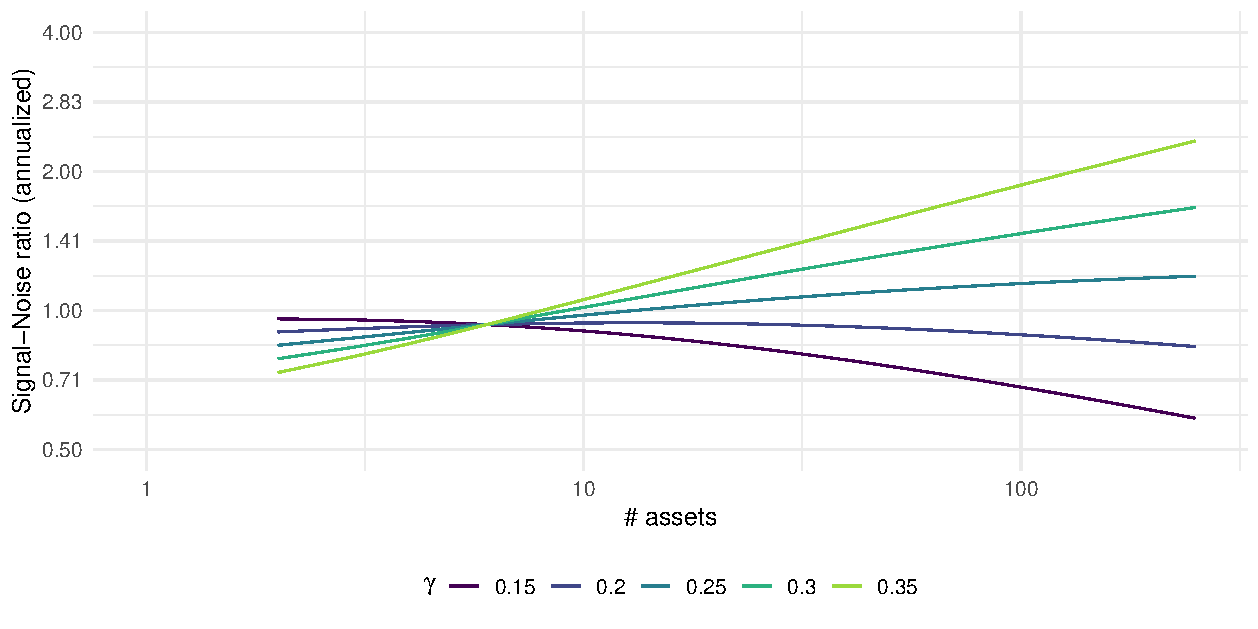
\includegraphics[width=0.99\textwidth,height=0.495\textwidth]{figure/qboundgrow_bound-1} \caption[The upper bound of \theoremref{qual_bound} is plotted versus \nlatf for different scaling laws.]{The upper bound of \theoremref{qual_bound} is plotted versus \nlatf for different scaling laws.}\label{fig:grow_bound}
\end{figure}

\end{knitrout}

The decreasing upper bound with respect to growing universe size
is illustrated in \figref{grow_bound}. Under the assumption
$\psnropt = \psnr[0]\nlatf^{\gamma}$, the upper bound
of \theoremref{qual_bound} is plotted versus \nlatf for 
different values of $\gamma$. 
The value of
$\psnr[0]$ is set so that 
$\psnropt=1.25\yrtomhalf$ when 
$\nlatf=6$.
For $\gamma < \oneby{4}$, one sees a local maximum in 
the upper bound as \nlatf increases, a behavior not seen for
$\gamma > \oneby{4}$, where the bound on \txtQual
grows with \nlatf. 


%$\psnropt$ and the $0.25, 0.50,$ and $0.75$ quantiles of
%$\psnropt\pql{\sportwfnc{\mreti}}$, under 
%\apxref{qual_dist}, are plotted versus \nlatf.
%The panels represent $\gamma$ values of
%$sort(pgammas)[1:(length(pgammas)-1)],$ and 
%$sort(pgammas)[length(pgammas)]$.
%The value of
%$\psnr[0]$ is set so that 
%$\psnropt=sqrt(ope)*zeta.s\yrtomhalf$ when 
%$\nlatf=n.stok$.
%For $\gamma < 0.25$, one sees a local maximum in 
%achieved \txtSR as \nlatf increases, a behavior not seen for
%$\gamma > 0.25$, where achieved \txtSR grows with \nlatf. 
%For the case of `slow growth' of \psnropt, the diversification 
%benefit is not seen by the sample \txtMP, rather its practical
%utility \emph{decreases} because the haircut outpaces the growth
%of \psnropt. As a practical matter, this may explain why the
%\txtMP is typically applied to small asset universes.



This relationship between \txtQual and \nlatf for different
values of $\gamma$ appears not just in the upper bound of
\theoremref{qual_bound}, but apparently also for most quantiles
of the distribution given by \apxref{qual_dist}, as
%This loss in value with respect to growing universe size is
illustrated in \figref{grow_sqrt}. Again assuming
$\psnropt = \psnr[0]\nlatf^{\gamma}$, lines of 
$\psnropt$ and the $0.25, 0.50,$ and $0.75$ quantiles of
$\psnropt\pql{\sportwfnc{\mreti}}$, under 
\apxref{qual_dist}, are plotted versus \nlatf.
The panels represent $\gamma$ values of
$0.15, 0.2, 0.25, 0.3,$ and 
$0.35$.
Again, the value of
$\psnr[0]$ is set so that 
$\psnropt=1.25\yrtomhalf$ when 
$\nlatf=6$.
For $\gamma < \oneby{4}$, one sees a local maximum in 
\txtQual as \nlatf increases, a behavior not seen for
$\gamma > \oneby{4}$, where quantiles of \txtQual grow with \nlatf. 
For the case of `slow growth' of \psnropt, the diversification 
benefit is not seen by the sample \txtMP, rather its practical
utility \emph{decreases} because the estimation error 
outpaces the growth of \psnropt. 

%Via the equivalence in \eqnref{sufficient_growth}, for the 
%bound \qbnd to be growing with respect to \nlatf, it suffices
%to establish that 
%$\half \le \wrapParens{\nlatf-1}\dbyd{\log\psnrsqopt}{\nlatf}$.
%From \eqnref{capm_zetas}, we have
%\begin{equation*}
%\begin{split}
%\half\dbyd{\log\psnrsqopt}{\nlatf} 
%&= 
%\frac{\trAB{\vect{\alpha}}{\dbyd{\vect{\alpha}}{\nlatf}} + 
%\wrapParens{\frac{\sigma_m}{\sigma}}^2 \wrapBracks{
 %\trAB{\vect{\beta}}{\dbyd{\vect{\beta}}{\nlatf}}\gram{\vect{\alpha}}
%+ \trAB{\vect{\alpha}}{\dbyd{\vect{\alpha}}{\nlatf}}\gram{\vect{\beta}}
%- \trAB{\vect{\alpha}}{\vect{\beta}}\wrapParens{
  %\trAB{\vect{\alpha}}{\dbyd{\vect{\beta}}{\nlatf}} + 
  %\trAB{\vect{\beta}}{\dbyd{\vect{\alpha}}{\nlatf}}}}}{%
%\gram{\vect{\alpha}} +
%\wrapParens{\frac{\sigma_m}{\sigma}}^2 \wrapBracks{%
%\gram{\vect{\beta}}\gram{\vect{\alpha}} -
%\wrapParens{\trAB{\vect{\alpha}}{\vect{\beta}}}^2}}
%+ \frac{\sigma_m^2 \trAB{\vect{\beta}}{\dbyd{\vect{\beta}}{\nlatf}}}{%
%\sigma^2 + \sigma_m^2\gram{\vect{\beta}}}.
%\end{split}
%\end{equation*}
%2FIX: where you going with this?
%These plots are built using \apxref{hcut_apx} ...

\subsection{Diversification under CAPM}%FOLDUP

It is not clear how \psnropt `should' scale with \nlatf. It is
easy to construct a model under which \psnropt scales as
$\nlatf^{\half}$: assume all assets have independent returns with
the same \txtSNR. It is also easy to accidentally construct 
a model under which \psnropt ultimately scales 
as $\nlatf^{\epsilon}$ for small $\epsilon$, as done here.
Suppose the \kth{i} asset has expected return
$\alpha_i$, exposure $\beta_i$ to `the market', and volatility
$\sigma$. Assume the market return is zero mean with volatility
$\sigma_m$. Then the squared \txtSNR is
\begin{align}
\nonumber
\psnrsqopt 
&= 
\frac{\gram{\vect{\alpha}} +
\wrapParens{\frac{\sigma_m}{\sigma}}^2 \wrapBracks{%
\gram{\vect{\beta}}\gram{\vect{\alpha}} -
\wrapParens{\trAB{\vect{\alpha}}{\vect{\beta}}}^2}}{\sigma^2 +
\sigma_m^2\gram{\vect{\beta}}},&\\
&= 
\frac{\gram{\vect{\alpha}}}{\sigma^2}
\frac{\sigma^2 + \sigma_m^2 \gram{\vect{\beta}} \fsin[2]{\psi}}{%
\sigma^2 + \sigma_m^2\gram{\vect{\beta}}},&
\label{eqn:capm_zetas}
\end{align}
where $\psi$ is the angle between the vectors \vect{\alpha}
and \vect{\beta}.
Depending on how the sine of $\psi$ grows with universe size, 
one observes different scaling of \psnropt with respect to \nlatf. When
the assets all have the same alpha and beta, \ie
$\vect{\alpha} = \alpha\vone$ and $\vect{\beta} = \beta\vone$,
the sine is identically zero, and 
$\psnropt = \sqrt{\fraccp{\nlatf\alpha^2}{\sigma^2 + \nlatf\sigma_m^2\beta^2}}
< \alpha\beta^{-1}\sigma_m^{-1}$. Thus 
\psnropt asymptotically scales slower than $\nlatf^{\epsilon}$
for all $\epsilon > 0$.

On the other hand, when the sine is
one, \ie when \vect{\alpha} is orthogonal to \vect{\beta},
$\psnropt = \sqrt{\gram{\vect{\alpha}}} \sigma^{-1}$, which
grows however the assets are ordered, presumably on the
order of $\nlatf^{\half}$. Thus under a CAPM model, the
growth of \psnropt depends on the `alignment' of the
vectors \vect{\alpha} and \vect{\beta}.
%UNFOLD

%UNFOLD

%%%%%%%%%%%%%%%%%%%%%%%%%%%%%%%%%%%%%%%%%%%%%%%%%%%%%%%%%%%%%%%%%%%%%%%%
\section{Generalizations}%FOLDUP

\label{sec:generalizations}

\theoremref{qual_bound} is somewhat lacking because it ignores conditioning
information which may affect the distribution of future returns, and which
may inform the portfolio manager. Few active managers, it is presumed,
are holding the unconditional \txtMP based on in-sample data. What is sought
is a more general theorem that allows more elaborate models of returns,
and more elaborate, parametrized, trading schemes, with \psnropt redefined 
as the maximal portfolio \txtQual over the trading schemes, and \nlatf
redefined as the `degrees of freedom', perhaps the rank of some derivative
at the optimal parameter, say. Towards that goal, a few generalizations can
easily be made.

\subsection{Conditional portfolio \txtQual}%FOLDUP
\label{subsec:cond_portfolio_qual}

The model of stationary mean returns is generalized by one where
the expected return of the assets is linear in some state
variables, or `features', \vfact[i], observed prior to the investment
decision.  \cite{pav_the_book,connor1997,herold2004TAA} That
is, one observes the \nfac-vector $\vfact[i]$ at some time prior to 
when the investment decision is required to capture \vreti[i+1]. 
The general model is now
\begin{align}
\label{eqn:cond_model_IV}
\Econd{\vreti[i+1]}{\vfact[i]} &=
\pRegco \vfact[i], &
\Varcond{\vreti[i+1]}{\vfact[i]} &=
\pvsig,
\end{align}
where \pRegco is some \bby{\nlatf}{\nfac} matrix. 

Here we bound the \txtQual of portfolios which are
linear in the features \vfact[i]. That is, the portfolio
manager allocates their assets proportional to
$\sportW\vfact[i]$ for some matrix $\sportW$.

Using the law of iterated expectations, the unconditional
expected value of the returns of the portfolio is
\begin{equation*}
\E{\Econd{\trAB{\wrapParens{\sportW\vfact[i]}}{\vreti[i+1]}}{\vfact[i]}}
= \trace{\tr{\sportW}\pRegco\E{\ogram{\vfact[i]}}}
= \trace{\tr{\sportW}\pRegco\pfacsig},
\end{equation*}
by definition of \pfacsig as the second moment of \vfact[i].

Unfortunately the unconditional variance will, in general,
involve a term quadratic in the expectation. However, it
can easily be shown that the unconditional \emph{expected} 
variance of the portfolio's returns is
\begin{equation*}
\E{\qform{\pvsig}{\wrapParens{\sportW\vfact[i]}}} =
\trace{\qform{\pvsig}{\sportW}\pfacsig}.
\end{equation*}
We can then redefine\footnote{If an analysis of the conditional expected
return divided by risk is required, it is possible one could define
\pQl{\cdot} as the expected return divided by square root of the unconditional
second moment. The \txtQual would then be $\ftan{\farcsin{\pQl{\cdot}}}$.
One could possibly find a \txtCR bound on the expected value of this \pQl{\cdot}.
This `Pillai-Bartlett' form of \pQl{\cdot} is likely unrequired for low frequency
settings.} the \txtQual of the portfolio as the
unconditional mean divided by the unconditional expected risk:
\begin{equation}
\pQl{\sportW}\defeq\frac{\trace{\tr{\sportW}\pRegco\pfacsig}}{%
\sqrt{\trace{\qform{\pvsig}{\sportW}\pfacsig}}}.
\end{equation}
When \vfact[i] is a deterministic scalar constant, 
this coincides with the `usual' definition of \txtQual as being 
like a \txtSR. However, except possibly for an intercept term, one
expects \vfact[i] to be random, or at least out of the control of
the portfolio manager.

Once again, a risk transform can be injected to express
portfolio optimization as an estimation problem on a sphere:
\begin{equation}
\begin{split}
\pQl{\sportW}
&=\frac{\trace{\trAB{%
\wrapParens{\trchol{\pvsig}\sportW\chol{\pfacsig}}}{%
\wrapParens{\ichol{\pvsig}\pRegco\chol{\pfacsig}}}{%
}}}{%
\sqrt{\trace{
\gram{\wrapParens{\trchol{\pvsig}\sportW\chol{\pfacsig}}}}}},\\
&=
\frac{\trAB{\fvec{\trchol{\pvsig}\sportW\chol{\pfacsig}}}{%
\fvec{\ichol{\pvsig}\pRegco\chol{\pfacsig}}}}{%
\sqrt{\gram{\fvec{\trchol{\pvsig}\sportW\chol{\pfacsig}}}}}.
\end{split}
\end{equation}
This function is maximized by taking
\begin{equation}
\sportW = \pportWopt \defeq \minv{\pvsig}{\pRegco},
\end{equation}
which has \txtQual
\begin{equation}
\psnropt\defeq\pQl{\pportWopt} =
\sqrt{\trace{\qiform{\pvsig}{\pRegco}\pfacsig}}.
\end{equation}
The square of this quantity, \psnrsqopt, 
is the `population analogue' of the Hotelling-Lawley trace. \cite{Rencher2002,Muller1984143}

Again we can write
\begin{equation*}
\frac{\pQl{\sportW}}{\psnropt} = 
\trAB{\fnorm{\fvec{\trchol{\pvsig}\sportW\chol{\pfacsig}}}}{%
\fnorm{\fvec{\ichol{\pvsig}\pRegco\chol{\pfacsig}}}}.
\end{equation*}
Thus finding a `good' \sportW becomes an estimation problem on the
sphere \sphere{\nfac\nlatf - 1}. An analogue
to \theoremref{qual_bound} can be proved with $\nfac\nlatf$ replacing
$\nlatf$, by assuming a particular form to the likelihood. We must
generalize the assumption of Directional Independence, after which
the theorem proceeds easily.

\begin{assumption}[Conditional Directional Independence]%FOLDUP
Assume that
\begin{equation}
\label{eqn:sane_estimator_cond}
\E{\fnorm{\fvec{\trchol{\pvsig}\sportWfnc{\mreti,\mfact}}}} = 
\cfnc{\psnrsqopt} \fnorm{\fvec{\trchol{\pvsig}\pportWopt\chol{\pfacsig}}}
+ \Bterm,
\end{equation}
where \Bterm is the bias term, orthogonal to 
\fnorm{\fvec{\trchol{\pvsig}\pportWopt\chol{\pfacsig}}}.
\end{assumption}%UNFOLD

\begin{theorem}%FOLDUP
\label{theorem:qual_bound_two}
Let one element of \vfact[i] be a deterministic $1$. Suppose the
vector of the remaining $\nfac-1$ elements of \vfact[i] stacked 
on top of \vreti[i+1] are multivariate Gaussian.  Let \mreti, 
\mfact be \bby{\ssiz}{\nlatf} and \bby{\ssiz}{\nfac} matrices
of \iid observations of the features and returns.
Let \sportWfnc{\mreti,\mfact} be an estimator 
%based on 
%\ssiz \iid observations of multivariate Gaussian returns, \mreti, 
%and multivariate Gaussian features, \mfact, with one column of \mfact
%an intercept term, 
satisfying the assumptions of
Conditional Directional Independence and Residual Independence. Then
\begin{equation}
\E{\pQl{\sportWfnc{\mreti,\mfact}}} 
\le \frac{\sqrt{\ssiz}\psnrsqopt}{\sqrt{\nfac\nlatf - 1 + \ssiz\psnrsqopt}}.
\end{equation}
\end{theorem}%UNFOLD
\begin{proof}%FOLDUP

We can proceed as in \secref{portfolio_qual}. Let \mreti be the 
\bby{\ssiz}{\nlatf} matrix of portfolio returns, and let 
\mfact be the corresponding \bby{\ssiz}{\nfac} matrix of features.
View the portfolio coefficient \sportW as an estimator, a function of
the random data, \ie \sportWfnc{\mreti,\mfact}.
%Assume
%Directional Independence, with \eqnref{sane_estimator}
%becoming
%\begin{equation}
%\E{\fnorm{\trchol{\pvsig}\sportWfnc{\mreti,\mfact}}} = 
%\cfnc{\psnrsqopt} \fnorm{\trchol{\pvsig}\pportWopt\chol{\pfacsig}}
%+ \Bterm.
%\end{equation}
Define
\begin{equation}
\prskMtx\defeq{\ichol{\pvsig}\pRegco\chol{\pfacsig}}.
\end{equation}
Then 
\begin{equation*}
\psnrsqopt = \trace{\gramprskMtx}.
\end{equation*}

We get, analogously to \eqnref{crb_one},
\begin{equation}
\oneby{\ssiz}\trace{\qoform{\iFishI[\fvec{\prskMtx}]}{\Drv}}
\le 1 - \csqfnc{\trace{\gramprskMtx}},
\end{equation}
where
\begin{equation}
\Drv\defeq
{\dbyd{\cfnc{\trace{\gramprskMtx}}\frac{\prskMtx}{\sqrt{\trace{\gramprskMtx}}}}{\fvec{\prskMtx}}}.
\end{equation}

Without loss of generality, we assume it is the first element
of \vfact[i] that is a deterministic $1$. Then, the log likelihood of 
the vector of $\vfact[i]$ stacked on top of $\vreti[i+1]$
is: \cite{pav2013markowitz}
\begin{equation}
\label{eqn:cond_llik_one}
\log \FOOlik{}{\pvsm}{\twobyone{\vfact[i]}{\vreti[i+1]}} = 
  c_{\nfac+\nlatf} 
- \half \logdet{\pvsm} 
- \half \trace{\minv{\pvsm}\ogram{\twobyone{\vfact[i]}{\vreti[i+1]}}},
\end{equation}
where \pvsm is the second moment matrix:
\begin{equation}
\pvsm \defeq \E{\ogram{\twobyone{\vfact[i]}{\vreti[i+1]}}}
= \twobytwo{\pfacsig}{\pfacsig\tr{\pRegco}}{\pRegco\pfacsig}{\pvsig +
\qoform{\pfacsig}{\pRegco}}.
%\qoform{\pfaccov}{\pRegco}}}.
\end{equation}
The inverse of \pvsm has the following, somewhat surprising, form \cite{pav2013markowitz}:
\begin{equation}
\minv{\pvsm} 
= \twobytwo{\minv{\pfacsig} +
\qiform{\pvsig}{\pRegco}}{-\tr{\pRegco}\minv{\pvsig}}{-\minv{\pvsig}\pRegco}{\minv{\pvsig}}.
\end{equation}
A square root of this matrix (a Cholesky factor, up to permutation)
is:
\begin{equation}
\begin{split}
\minv{\pvsm} &=
\ogram{%
\twobytwo{\ichol{\pfacsig}}{-\tr{\pRegco}\ichol{\pvsig}}{\mzero}{\ichol{\pvsig}}
},\\
&= \twobytwo{\ichol{\pfacsig}}{\mzero}{\mzero}{\eye}
\ogram{%
\twobytwo{\eye}{-\prskMtxU{\trsym}}{\mzero}{\ichol{\pvsig}}}
\twobytwo{\trichol{\pfacsig}}{\mzero}{\mzero}{\eye}.
\end{split}
\end{equation}

By the block determinant formula, 
\begin{equation}
\det{\pvsm} 
= \det{\pfacsig}\det{\pvsig + \qoform{\pfacsig}{\pRegco} -
\pRegco\pfacsig\minv{\pfacsig}\pfacsig\tr{\pRegco}}
= \det{\pfacsig}\det{\pvsig}.
\end{equation}
Thus, conditional on \pfacsig and \pvsig, the negative log likelihood
takes the form:
\begin{multline}
\label{eqn:cond_llik_two}
- \log \FOOlik{}{\prskMtx, \pfacsig, \pvsig}{\twobyone{\vfact[i]}{\vreti[i+1]}} = 
- c_{\nfac+\nlatf}
+ \half \logdet{\pfacsig} 
+ \half \logdet{\pvsig}\\
+ \half \trace{
\ogram{%
\twobytwo{\eye}{-\prskMtxU{\trsym}}{\mzero}{\ichol{\pvsig}}}
\ogram{\twobyone{\trichol{\pfacsig}\vfact[i]}{\vreti[i+1]}}}.
\end{multline}
Sweeping the nuisance parameter terms into the constant, as well
as terms in the trace which are not quadratic in \prskMtx, we
have 
\begin{align}
\label{eqn:cond_llik_three}
- \log \FOOlik{}{\prskMtx, \pfacsig, \pvsig}{\twobyone{\vfact[i]}{\vreti[i+1]}}
&= - c'
+ \half \trace{\gramprskMtx 
\ogram{\wrapParens{\trichol{\pfacsig}\vfact[i]}}},&\\
&= - c'
+ \half
\tr{\fvec{\prskMtx}}\fvec{\prskMtx\trichol{\pfacsig}\ogram{\vfact[i]}\ichol{\pfacsig}}.&\\
&= - c'
+ \half
\tr{\fvec{\prskMtx}}\wrapParens{%
\wrapBracks{\trichol{\pfacsig}\ogram{\vfact[i]}\ichol{\pfacsig}}
 \kron \eye}\fvec{\prskMtx}.&
\end{align}
The Fisher Information, then, is
\begin{equation}
\FishI[\fvec{\prskMtx}] =
\E{\wrapParens{%
\wrapBracks{\trichol{\pfacsig}\ogram{\vfact[i]}\ichol{\pfacsig}}
 \kron \eye}} = \eye[\nfac\nlatf].
\end{equation}

The remainder of the proof proceeds exactly as in 
\secref{portfolio_qual}. 
\end{proof}%UNFOLD

%\begin{theorem}
%\label{theorem:qual_bound_two}
%Let \sportWfnc{\mreti,\mfact} be an estimator based on 
%\ssiz \iid observations of multivariate Gaussian returns, \mreti, 
%and multivariate Gaussian features, \mfact, with one column of \mfact
%an intercept term, satisfying the assumptions of
%directional independence and residual independence. Then
%\begin{equation}
%\E{\pQl{\sportWfnc{\mreti,\mfact}}} 
%\le \frac{\sqrt{\ssiz}\psnrsqopt}{\sqrt{\nlatf\nfac - 1 + \ssiz\psnrsqopt}}.
%\end{equation}
%\end{theorem}

%&= \E{\Cmat\scoro{\prskvec}{\FOOlik{}{\prskvec}{\mreti}}

%\begin{equation}
%\begin{split}
%\vfact[i] &\sim \normlaw{\pfacmu, \pfaccov},\\
%\condtwo{\vreti[i+1]}{\vfact[i]} &\sim \normlaw{\pRegco\vfact[i], \pvsig}.
%\end{split}
%\end{equation}
%Together the unconditional distribution is
%\begin{equation}
%\twobyone{\vfact[i]}{\vreti[i+1]} \sim
%\normlaw{\twobyone{\pfacmu}{\pRegco\pfacmu}, 
%\twobytwo{\pfaccov}{\pfaccov\tr{\pRegco}}{\pRegco\pfaccov}{\pvsig +
%\qoform{\pfaccov}{\pRegco}}}.
%\end{equation}




%In this model, the `Markowitz Coefficient' 
%$\minvAB{\pvsig}{\pRegco}$, generalizes the \txtMP as
%the coefficient of the optimal portfolio which is linear in \vfact,
%under some objective. \cite{pav2013markowitz} How should we define
%the \txtQual of the Markowitz Coefficient, and can we prove
%an analogue of \theoremref{qual_bound}?
%UNFOLD

\subsection{Subspace constraints}%FOLDUP

Consider, now, the case of conditional expectation, as presented in
\subsecref{cond_portfolio_qual}, but where the portfolio is 
constrained to be in some lower dimensional subspace. That is, by design, 
\begin{equation}
\zerJc \sportWfnc{\mreti,\mfact} = \vzero,
\end{equation}
where $\zerJc$ is a \bby{\wrapParens{\nlatf - \nlatfzer}}{\nlatf}
matrix of rank $\nlatf - \nlatfzer$, that is chosen independently
of the observations of \mreti and \mfact.
Let the rows of \zerJ span the null space of the rows of
\zerJc; that is, $\zerJc \tr{\zerJ} = \mzero$, and $\ogram{\zerJ} = \eye$.

We can simply use the results of \subsecref{cond_portfolio_qual}, but
replacing the assets with the \nlatfzer assets spanned by the rows of
\zerJ. That is, we can replace the \vreti[i+1] with $\zerJ\vreti[i+1]$,
and replace \sportWfnc{\mreti,\mfact} with
$\tr{\zerJ}\minv{\wrapParens{\ogram{\zerJ}}}\sportWfnc{\mreti,\mfact}$
to arrive at the following analogue of \theoremref{qual_bound_two}:

\begin{theorem}%FOLDUP
\label{theorem:qual_bound_three}
Let one element of \vfact[i] be a deterministic $1$. Suppose the
vector of the remaining $\nfac-1$ elements of \vfact[i] stacked 
on top of \vreti[i+1] are multivariate Gaussian.  Let \mreti, 
\mfact be \bby{\ssiz}{\nlatf} and \bby{\ssiz}{\nfac} matrices
of \iid observations of the features and returns.
Let \sportWfnc{\mreti,\mfact} be an estimator 
%based on 
%\ssiz \iid observations of multivariate Gaussian returns, \mreti, 
%and multivariate Gaussian features, \mfact, with one column of \mfact
%an intercept term, 
satisfying the assumptions of
directional independence and residual independence, with the constraint
\begin{equation}
\zerJc \sportWfnc{\mreti,\mfact} = \vzero,
\end{equation}
for \bby{\wrapParens{\nlatf - \nlatfzer}}{\nlatf} matrix \zerJc, which
is chosen independently of the observed \mreti and \mfact. 
Let the rows of \zerJ span the null space of the rows of
\zerJc. 

Then
\begin{equation}
\E{\pQl{\sportWfnc{\mreti,\mfact}}} 
\le \frac{\sqrt{\ssiz}\psnrsqoptG{\zerJ}}{\sqrt{\nfac\nlatfzer - 1 +
\ssiz\psnrsqoptG{\zerJ}}},
\end{equation}
where 
\begin{equation*}
\psnrsqoptG{\zerJ}\defeq 
\trace{\qform{\wrapProj{\pvsig}{\zerJ}}{\pRegco}\pfacsig}.
\end{equation*}
\end{theorem}%UNFOLD
%UNFOLD

\subsection{Hedging constraints}%FOLDUP

Consider, now, the case where one seeks a portfolio whose returns are
independent, in the probabilistic sense, of the returns of some 
traded instruments in the investment universe. 
Independence is a difficult property to
check or enforce; however, independence implies zero covariation, which
can be easily formulated and checked. 

Since the portfolio estimator may not deliver a perfectly
hedged portolio due to misestimation of the covariance matrix, we
will, with perfect knowledge of \pvsig, consider the \txtQual of the 
hedged part of the portfolio. The hedged
part is defined in terms of a risk projection. 
If \sportw[1] is a feasible portfolio based on the sample,
then the hedged version of this portfolio is the solution to the
optimization problem
\begin{equation}
\min_{\sportw : \hejG\pvsig\sportw = \vzero} \VAR{\trAB{\wrapParens{\sportw -
\sportw[1]}}{\vreti[i+1]}},
\end{equation}
where $\hejG$ is a \bby{\nlatfhej}{\nlatf} matrix of 
rank \nlatfhej, the rows of which we wish to `hedge out.'

Using the Lagrange multiplier technique, this can easily be found to
be solved by 
\begin{equation}
\sportw = \sportw[1] - \wrapProj{\pvsig}{\hejG}\pvsig\sportw[1].
\end{equation}
Thus we will consider the \txtQual of the portfolio estimator
\begin{equation*}
\wrapParens{\eye[\nlatf] - \wrapProj{\pvsig}{\hejG}\pvsig}\sportWfnc{\mreti,\mfact}.
\end{equation*}
Note, however, that the row rank of
$\wrapParens{\eye[\nlatf] - \wrapProj{\pvsig}{\hejG}\pvsig}$ 
is $\nlatf - \nlatfhej$.  Thus hedging is an instance of a subspace
constraint and we can apply \theoremref{qual_bound_three} outright.

\begin{theorem}%FOLDUP
\label{theorem:qual_bound_four}
Let one element of \vfact[i] be a deterministic $1$. Suppose the
vector of the remaining $\nfac-1$ elements of \vfact[i] stacked 
on top of \vreti[i+1] are multivariate Gaussian.  Let \mreti, 
\mfact be \bby{\ssiz}{\nlatf} and \bby{\ssiz}{\nfac} matrices
of \iid observations of the features and returns.
Let \sportWfnc{\mreti,\mfact} be an estimator 
%based on 
%\ssiz \iid observations of multivariate Gaussian returns, \mreti, 
%and multivariate Gaussian features, \mfact, with one column of \mfact
%an intercept term, 
satisfying the assumptions of
directional independence and residual independence. 
Let \bby{\nlatfhej}{\nlatf} matrix \hejG be chosen
independently of \mreti and \mfact. 

%2FIX: redefine Deltapsnr to not be confusing.
Define 
\begin{equation}
\Delpsnrsqopt{\eye,\hejG}
\defeq
\trace{\qiform{\svsig}{\pRegco}\pfacsig} - 
\trace{\qform{\wrapProj{\pvsig}{\hejG}}{\pRegco}\pfacsig}.
\end{equation}

Then
\begin{equation}
\E{\pQl{%
\wrapBracks{\eye[\nlatf] - \wrapProj{\pvsig}{\hejG}\pvsig}\sportWfnc{\mreti,\mfact}}} 
\le \frac{\sqrt{\ssiz}\Delpsnrsqopt{\eye,\hejG}}{\sqrt{\nfac\wrapParens{\nlatf -
\nlatfhej} - 1 + \ssiz\Delpsnrsqopt{\eye,\hejG}}}.
\end{equation}
\end{theorem}%UNFOLD

%UNFOLD

%UNFOLD

%%%%%%%%%%%%%%%%%%%%%%%%%%%%%%%%%%%%%%%%%%%%%%%%%%%%%%%%%%%%%%%%%%%%%%%%
\section{Examples}%FOLDUP

\subsection{The equal weight puzzle}%FOLDUP


\theoremref{qual_bound} can help us make sense of puzzling findings
in the literature. For example, in the ``$1/N$'' paper, DeMiguel \etal
find that the equal-weighting portfolio outperforms, in terms of out-of-sample
\txtSR (and other measures), the \txtMP and numerous other portfolio
estimators.  \cite{demiguel2009optimal}
This finding is supported on a number of real world data
sets, and a few synthetic ones. One data set used was the returns of
the 10 industry portfolios and the US equity market portfolio, computed
by Ken French. 
% 2FIX: add citation to data.

The monthly returns, from 1927-01-01 to 
2020-12-01, for these 10 
assets were downloaded
from Kenneth French's data library.  \cite{French10Port}
%from \emph{Quandl}.  \cite{Quandl}
The \txtSR of the equal weighted portfolio on the %10
assets, over the 1128 months, is around 
$0.67\yrtomhalf$. The \txtSR of the sample \txtMP over
the 10 assets over the same period is around
$0.86\yrtomhalf$.  
Now consider a portfolio estimator
given 5 years of observations, as in 
DeMiguel \etal \cite{demiguel2009optimal}, assuming 
$\psnropt=0.86\yrtomhalf$.
The bound on expected value of \pql{\sportwfnc{\mreti}} from \theoremref{qual_bound} is only $0.46\yrtomhalf$.  
%Under \apxref{qual_dist}, the probability that \pql{\sportwfnc{\mreti}} exceeds $sr1$sr\yrtomhalf$ in this case is only $dfp$. 
It is not surprising that DeMiguel \etal drew
the conclusions they did, nor that they would be refuted
by looking at a longer sample, as by Kritzman \etal \cite{defoopt2010}



One could also use \theoremref{qual_bound_four} here. However,
the upper bound of that theorem is non-negative, and zero only
if the quantity \Delpsnrsqopt{\eye,\hejG} is zero.  This is a
statement regarding unknown population parameters, but we can
perform inference on this quantity. For example, based on the
1128 months of data on these 
10, the 95\% confidence interval on
\Delpsnrsqopt{\eye,\hejG}, where \hejG is the \bby{1}{10}
matrix of all ones, is
$\asrowvec{0.04, 0.45}\yrto{-1}$, under the assumption of
Gaussian returns.  

%One could view the touted superiority of the equal weight portfolio
%over \eg the \txtMP as a veiled claim that there is a single
%discount factor that rules all asset returns. As stated, this claim
%is clearly absurd, since \eg an equal weight portfolio on both pairs
%of leveraged ETFs is clearly inferior to a portfolio equal weight \emph{short}
%both pairs.  \cite{zhang2010path}

%This highlights
%the fact that the putative superiority of the equal weight portfolio
%may be based on two due less to deficiencies in \eg the \txtMP, and more to
%the 

%The analysis presented here is likely to be optimistic when one
%considers the \emph{spanning} aspect of this problem.  
%\cite{giri1964likelihood,HKspan1987,KanZhou2012} That is, the
%total effect size beyond the equal weighting subspace may be
%very small. A `proper' analysis would take into account the
%difference in effect sizes and differences in universe size. 
%However, the spanning analogue of \theoremref{qual_bound}
%has not yet been established.

%% 2FIX: talk about the spanning statistics here. is there
%% any effect to exploit?
%The result is dKRS or
%dUNB or
%dMLE.
%the upper bound is asqb.
%Show it as:
%dsr2
%or cis: myci.

%UNFOLD

\subsection{Empirical diversification in the S\&P 100}%FOLDUP



To check how \psnropt \emph{might} scale with \nlatf, the weekly
log returns of the adjusted close prices of the stocks in the 
S\&P 100 Index, as of March 21, 2014, were downloaded 
from \emph{Quandl}.  \cite{Quandl} 
Adjustments for splits and
dividends were made in some unspecified way by the upstream source
of the data, Yahoo Finance. Stocks without a full 5 years of history
were discarded, leaving 96 stocks. 
Note that selection based on membership in the index at the end of the 
period adds no small amount of selection bias, which we shall ignore 
here.

Based on the weekly returns from 2009-03-27 to 2014-04-04,
estimates of \psnropt were computed, using the `KRS' estimator.
\cite{kubokawa1993estimation,pav_the_book} 
This was performed on the first \nlatf assets, with \nlatf ranging from 
$1$ to $96$.  The estimate of \psnropt versus \nlatf
is plotted in \figref{sp100_grow}, with assets added in alphabetical order.
Because Apple appears at the beginning of this list, it appears that
\psnropt starts reasonably large, but then actually \emph{decreases}
when adding assets. This is an artifact of the estimator, since the true
\psnropt can only increase when adding assets. 

\begin{knitrout}\small
\definecolor{shadecolor}{rgb}{0.969, 0.969, 0.969}\color{fgcolor}\begin{figure}[h]
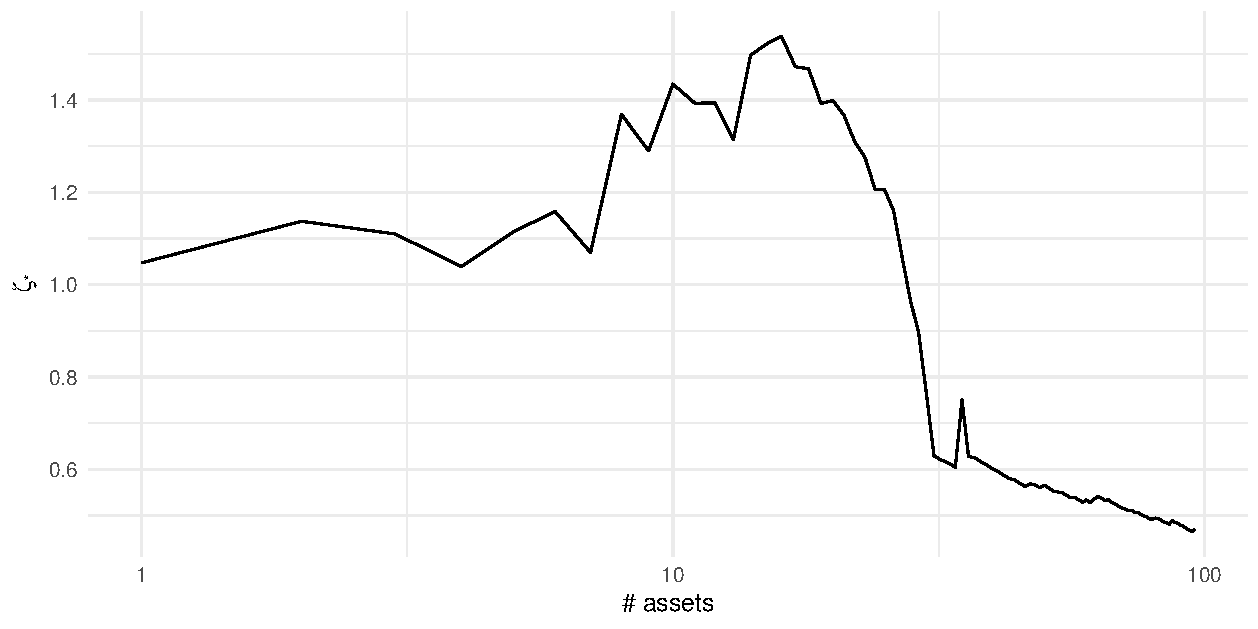
\includegraphics[width=0.99\textwidth,height=0.495\textwidth]{figure/qboundsp100_grow-1} \caption[Growth of estimated \psnropt versus \nlatf for the S\&P 100 Index names, in alphabetical order, showing the `Apple effect.']{Growth of estimated \psnropt versus \nlatf for the S\&P 100 Index names, in alphabetical order, showing the `Apple effect.'}\label{fig:sp100_grow}
\end{figure}

\end{knitrout}

%<<'sp100_mid',eval=TRUE,cache=FALSE,fig.width=5.75,fig.height=3.75,dpi=450,fig.cap=paste0("Growth of estimated \\psnropt versus \\nlatf for the S\\&P 100 Index names."),eval.after='fig.cap'>>= 

%foo.df <- data.frame(df=(1:length(KRSs)),KRS=KRSs,
		%MLE=MLEs,meanKRS=rowMeans(buncho.KRSs))

%require(ggplot2)
%ph <- ggplot(data=foo.df,aes(x=df,y=meanKRS))
%ph <- ph + geom_line()
%ph <- ph + labs(x="# assets",
								%y=expression(zeta["*"]))
%ph <- ph + scale_x_log10()
%ph <- ph + scale_y_log10()
%print(ph)

%@

Since the ordering of assets here is arbitrary, the experiment was repeated
1000 times, with the stocks randomly permuted, and 
\psnropt estimated as a function of \nlatf. Boxplots, over the
1000 simulations, of the KRS statistic versus
\nlatf are given in \figref{sp100_box}. There is effectively no 
diversification benefit observed here beyond the mean effect, which is
equivalent to holding an equal weight portfolio. Given the 
conditions under which \txtQual grows with \nlatf outlined in 
\secref{diversification}, one expects poor performance of 
directionally independent portfolio estimators
over even a small subset of the S\&P 100.

\begin{knitrout}\small
\definecolor{shadecolor}{rgb}{0.969, 0.969, 0.969}\color{fgcolor}\begin{figure}[h]
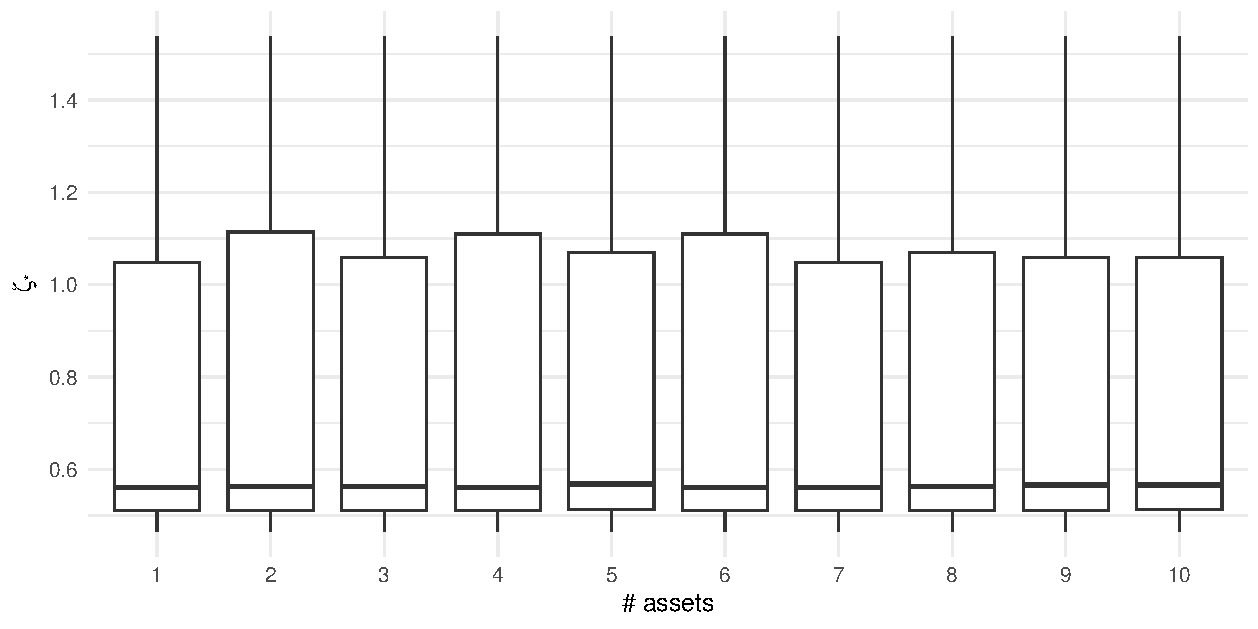
\includegraphics[width=0.99\textwidth,height=0.495\textwidth]{figure/qboundsp100_box-1} \caption[Growth of estimated \psnropt versus \nlatf for the S\&P 100 Index names is shown over 1000 permutations of the stocks, showing that there is effectively \emph{no} diversification benefit here beyond an equal weight portfolio]{Growth of estimated \psnropt versus \nlatf for the S\&P 100 Index names is shown over 1000 permutations of the stocks, showing that there is effectively \emph{no} diversification benefit here beyond an equal weight portfolio.}\label{fig:sp100_box}
\end{figure}

\end{knitrout}
%UNFOLD
%UNFOLD

%%%%%%%%%%%%%%%%%%%%%%%%%%%%%%%%%%%%%%%%%%%%%%%%%%%%%%%%%%%%%%%%%%%%%%%%
\section{Discussion}%FOLDUP

Care should be taken in the interpretation of \theoremref{qual_bound},
or its generalizations from \secref{generalizations}.
It does not claim that the sample \txtMP is somehow `optimal,' nor
does it make comparative claims about different portfolio estimators
when presented with the same data.
The theorem does not imply that somehow `overfitting' to the observed
data can be mitigated by selecting a less desireable portfolio. 
It does not claim that sample estimates of the \txtQual of a portfolio
are useless.  It is trivially
the case, for example, that if $\pql{\sportw[1]} > \pql{\sportw[2]}$, then,
with probability greater than half, 
$\trAB{\sportw[1]}{\svmu} / \sqrt{\qform{\svsig}{\sportw[1]}} > 
\trAB{\sportw[2]}{\svmu} / \sqrt{\qform{\svsig}{\sportw[2]}}$, where
the probability is over draws of \svmu and \svsig.
The theorem does not claim that the expected
\txtQual of a portfolio estimator is negative. (Indeed, it can not,
since the portfolio estimator which generates a random portfolio, 
ignoring the data, has zero expected \txtQual). 
The theorem makes no claims (\eg providing a Bayesian posterior) about 
any particular portfolio based on a single sample of the data: it is
a statement about the expectation of the \emph{estimator} under replication 
of draws of the sample.

One should recognize, moreover, there are situations where the assumptions
of the theorem are violated. For example, in some cases a prior 
bias for positive expected returns, \ie $\pvmu \ge 0$, is warranted,
and thus a portfolio estimator with a long bias is chosen.
This can happen when the underlying assets are equities, and
the eligible universe is based on some minimum longevity, as this 
introduces a `good' survivorship bias: 
companies with negative expected return should founder and perish, 
leaving behind those with more positive $\pmu$. Effectively this
acts to boost \ssiz somewhat, although the effect is likely small.

There are other reasonable portfolio estimators which violate the 
assumption of Directional Independence. For example, an estimator
which performs some dimensionality reduction based on the observed
data, \mreti and \mfact will not be covered by 
\theoremref{qual_bound_three} since the subspace is chosen based
on the sample. However, it might not be covered by 
\theoremref{qual_bound_two} because the expected \txtQual might
depend on how \pRegco aligns with the leading eigenvectors of
\pvsig, say.

\subsection{Future work}%FOLDUP

These findings perhaps raise more questions than they answer:
%This work leaves unanswered a number of interesting questions:
\begin{compactenum}
\item Foremost, the bounds of 
\theoremref{qual_bound} and \theoremref{qual_bound_two}
depend on the unknown
quantity, \psnrsqopt. How can we perform inference, 
Frequentist or Bayesian, on \pql{\sportwopt}, where \sportwopt is the \txtMP, 
given the observed information (\viz \svmu and \svsig)? This
is a problem of enormous practical concern to hundreds of
quantitative portfolio managers.

Contrast inference on the portfolio \txtQual with inference
on the population \txtSNR: under Gaussian returns, the
distribution of \ssrsqopt in terms of \ssiz, \nlatf and \psnrsqopt
is known. \cite[Theorem 5.2.2]{anderson2003introduction}
Thus, for example, the quantity
$\wrapParens{1 - \fracc{\nlatf}{\ssiz}}\ssrsqopt - \fracc{\nlatf}{\ssiz}$
is an unbiased estimator for \psnrsqopt, \etc 
Performing inverence on \pql{\sportwopt} is tricky because \psnrsqopt
is unknown and the error $\sportwopt - \pportwopt$ is likely
not independent of the error in the estimate \ssropt.

It may be the case, however, that inference on the portfolio
\txtQual qualifies as an `impossible' estimation-after-selection
problem. \cite{leeb2006}
\item While \theoremref{qual_bound} requires Gaussian returns, 
one expects that the result holds for returns distributions whose 
likelihood is ``more concave'' than the Gaussian at the MLE.
Exact conditions for this to hold should be established.
%\item How is \txtQual affected by the imposition of hedging and
%other constraints?  \cite{pav2013markowitz} Does dimensionality
%reduction modify the `degrees of freedom' in the straightforward
%way? Is there an analogue of the bound for portfolio
%spanning?  \cite{giri1964likelihood,HKspan1987,KanZhou2012}
%That is, can we find a bound on $\E{\pql{\sportw[2]} - \pql{\sportw[1]}}$,
%where \sportw[1] is a portfolio on a subspace of the assets over
%which \sportw[2] is selected, with the bound depending on the 
%spanning parameter, $\psnrsqoptG{2} - \psnrsqoptG{1}$?
\item \theoremref{qual_bound_two} applies to the case of 
trading strategies where the portfolio is linear in the 
observable features, \vfact[i]. 
Can it be used as an approximate bound for trading
strategies which are nonlinear, complex functions of the features?
\item What can be said about scaling of \psnropt with respect to
\nlatf for different models of market returns? Can one establish
sane sufficient conditions for which \psnropt grows slower than
$\nlatf^{\oneby{4}}$? What is the analogue of \eqnref{capm_zetas}
for a multi-factor model of returns?
%\item Can we find a lower bound, or a non-trivial upper bound on the 
%variance of $\pql{\sportwfnc{\mreti}}$? Together these could be used
%to give guarantees about the quantiles of \pql{\sportwfnc{\mreti}}.
%A lower bound on the variance can likely be had via a result of
%Kakarala and Watson. \cite{ANZS:ANZS253} Together with Cantelli's
%Inequality, these would give rough (perhaps useless) upper bounds
%on the 
%\kth{\qlev} quantile of portfolio \txtQual, for $\half < \qlev < 1$.
%\item The simulations of \secref{apx_distribution} should
%be repeated with different choices of \ssiz, \nlatf, and \psnropt.
\item How tight is the bound of \theoremref{qual_bound}, and can 
it be much improved by directly analyzing the differential
inequality of \eqnref{crb_three}, rather than discarding
the derivative term? Or perhaps the bound can be improved by using
an `intrinsic' \txtCR bound.  \cite{DBLP:conf/icassp/XavierB05}
%\item How good is \apxref{qual_dist}? Can we find the expected
%value of the distribution in \apxref{qual_dist}, and what is the
%gap between it and the bound of \theoremref{qual_bound}?
%Can we find the \emph{exact} distribution of \txtQual of the 
%sample \txtMP under Gaussian returns, 
%perhaps leveraging the work of Bodnar and Okhrin,
%or of Britton-Jones.  \cite{SJOS:SJOS729, BrittenJones1999}
\item Can the assumption of Directional Independence be weakened?
Can the \theoremref{qual_bound_two} be generalized to deal with omitted 
variable bias in \vfact[i]?  
\item The analysis of \txtQual ignores the `risk-free' or `disastrous'
rate of return, and all trading costs. Can the expected bounds
be generalized to include these costs?
\end{compactenum}
%UNFOLD
%UNFOLD

%%%%%%%%%%%%%%%%%%%%%%%%%%%%%%%%%%%%%%%%%%%%%%%%%%%%%%%%%%%%%%%%%%%%%%%%
% bibliography%FOLDUP
%\nocite{markowitz1952portfolio,markowitz1999early,markowitz2012foundations}
%\bibliographystyle{jss}
%\bibliographystyle{siam}
%\bibliographystyle{ieeetr}
%\bibliographystyle{plainnat}
\bibliographystyle{apacite}
%\bibliographystyle{acm}
\bibliography{SharpeR,rauto}
%UNFOLD

%%%%%%%%%%%%%%%%%%%%%%%%%%%%%%%%%%%%%%%%%%%%%%%%%%%%%%%%%%%%%%%%%%%%%%%%
\appendix%FOLDUP

\section{Miscellaneous Proofs}%FOLDUP
\label{sec:misc_proofs}

%UNFOLD

\section{Declaration of Interests}

The authors report no conflicts of interest.
The authors alone are responsible for the content and writing of the paper.

%UNFOLD

%It is trivial to show that for random variable $\vect{y}$,
%\E{\gram{\wrapParens{\vect{y} - \vect{z}}}} is minimized by
%$\vect{z} = \E{\vect{y}}$. Moreover, we have
%\begin{equation*}
%\begin{split}
%\E{\gram{\wrapParens{\vect{y} - \E{\vect{y}}}}} 
%&= \E{\trace{\gram{\wrapParens{\vect{y} - \E{\vect{y}}}}}},\\
%&= \trace{\E{\ogram{\wrapParens{\vect{y} - \E{\vect{y}}}}}},\\
%&= \trace{\VAR{\vect{y}}}.
%\end{split}
%\end{equation*}
%Thus, if we take the expectation
%of \eqnref{cos_law_form}, we can then bound the left hand
%side from below by the trace of the variance:
%\begin{equation}
%\begin{split}
%\trace{\VAR{\fnorm{\trchol{\pvsig}\sportwfnc{\mreti}}}} 
%&\le 2 - 2 \E{\frac{\pql{\sportwfnc{\mreti}}}{\psnropt}},\\
%&= 2 \wrapParens{1 -
%\trAB{{\E{\fnorm{\trchol{\pvsig}\sportwfnc{\mreti}}}}}{%
%\fnorm{\trchol{\pvsig}\pportwopt}}}.
%\label{eqn:var_bounds}
%\end{split}
%\end{equation}
%By bounding the variance via a \txtCR bound, we can find an
%upper bound on the expected value of \pql{\sportw}.

%Using the quadratic formula, we have
%\begin{equation}
%\cfnc{\gramprskvec} \le \frac{-\ssiz\gramprskvec +
%\sqrt{\ssiz^2\wrapParens{\gramprskvec}^2 + 2
%\ssiz\gramprskvec\wrapParens{\nlatf-1}}}{\nlatf - 1}.
%\end{equation}
%For $\ssiz\gramprskvec$ large, we have a cancellation of terms.
%Because the square root function is concave, it is less than its
%linear approximation about $\ssiz^2\wrapParens{\gramprskvec}^2$. 
%That is, we have $\sqrt{x + \epsilon} \le \sqrt{x} +
%\oneby{2\sqrt{x}}\epsilon$.
%Thus 
%\begin{equation}
%\cfnc{\gramprskvec} \le 1. \mbox{oops: 2FIX}
%\end{equation}

\end{document}
%for vim modeline: (do not edit)
% vim:fdm=marker:fmr=FOLDUP,UNFOLD:cms=%%s:syn=rnoweb:ft=rnoweb:et:nu
 words.

\newpage

\author{}

\maketitle


%%%%%%%%%%%%%%%%%%%%%%%%%%%%%%%%%%%%%%%%%%%%%%%%%%%%%%%%%%%%%%%%%%%%%%%%
\begin{abstract}%FOLDUP
The \txtQual of a portfolio of \nlatf assets, its expected return divided 
by its risk, is couched as an estimation problem on the sphere
\spherep.  
When a portfolio is built using noisy data and a general purpose method, 
the expected value of the \txtQual is bounded from above via a \txtCR bound, 
%on the portfolio estimator, 
for the case of Gaussian returns. 
% The bound holds for `biased' estimators, thus there appears to be no bias-variance tradeoff for the problem of maximizing the \txtQual. 
%An approximate distribution of the \txtQual for the \txtMP is given, and shown to be fairly accurate via Monte Carlo simulations, for Gaussian returns as well as more exotic returns distributions.
These findings imply that if the maximal population 
\txtSNR grows slower than the universe size to the 
\oneby{4} power, there may be no diversification benefit, 
rather expected \txtQual can \emph{decrease} with additional assets.
As a practical matter, this may explain why the
\txtMP is typically applied to small asset universes.
Finally, the theorem is expanded to cover more general models
of returns and trading schemes, including the conditional expectation
case where mean returns are linear in some observable
features, subspace constraints (\ie dimensionality reduction),
and hedging constraints.
\end{abstract}%UNFOLD

Keywords: Markowitz Portfolio, Portfolio Selection, Sharpe Ratio, Asset Management.\\

% Key Messages:
Practitioner points:
\begin{compactenum}
\item An upper bound on the expected \txtSR of the \txtMP is given.
\item The bound considers true effect size, observation history and number of decisions.
\item The upper bound quantifies ``overfitting'' in portfolio selection problems.
\end{compactenum}


%%%%%%%%%%%%%%%%%%%%%%%%%%%%%%%%%%%%%%%%%%%%%%%%%%%%%%%%%%%%%%%%%%%%%%%%
\section{Introduction}%FOLDUP

Given \nlatf assets with expected return \pvmu and covariance of return \pvsig,
the portfolio defined as 
\begin{equation}
\pportwopt \defeq \minvAB{\pvsig}{\pvmu},
\end{equation}
known, somewhat informally, as the `\txtMP',
plays a central role in portfolio 
theory. \cite{markowitz1952portfolio,brandt2009portfolio}
Up to scaling, it solves the classic mean-variance
optimization, as well as the 
(population) \txtSR maximization problem:
\begin{equation}
\max_{\pportw }
\frac{\trAB{\pportw}{\pvmu}}{\sqrt{\qform{\pvsig}{\pportw}}}.
\label{eqn:opt_port_I}
\end{equation}

Despite its theoretical superiority, 
in practice the \txtMP has a tarnished reputation, and
is infrequently, if ever, used without some modification.
The unknown population parameters \pvmu and \pvsig must be estimated from samples, resulting in a feasible portfolio of dubious value. 
Michaud went so far as to call mean-variance optimization, ``error maximization.'' \cite{michaud1989markowitz}  
In its stead, numerous portfolio construction methodologies have been proposed
to replace the \txtMP, 
some based on patching conjectured theoretical deficiencies, 
others relying on simple heuristics. \cite{demiguel2009optimal,tu2011markowitz,brandt2009portfolio}

Pratitioners often resort to dimensionality reduction heuristics
to mitigate estimation error, effectively reducing the number 
of free variables in the portfolio optimization problem. 
One version of this tactic describes the returns of
dozens, or even hundreds, of equities as the linear combination
of a handful of `factor' returns (plus some `idiosyncratic' term); 
the portfolio problem is then couched as an optimization over factor
portfolios. If the population parameters were known with certainty,
shrinking the set of feasible portfolios would only result in
reducing the optimal portfolio utility. However, the population
parameters can typically only be weakly estimated, and dimensionality
reduction is common practice. 

In this paper, an upper bound is established on the expected value of
a feasible portfolio's \txtQual, defined to be the expected return of the portfolio
divided by its risk, with return and risk measured using the (unknown)
population parameters, and with the ``expected value'' taken over realizations
of the sample used to estimate the portfolio. 
This bound balances the `effect size,' $\sqrt{\ssiz \qiform{\pvsig}{\pvmu}},$ with the number of assets,
\nlatf, and justifies some form of dimensionality reduction. 
It is established, for example, that if, by adding additional assets
to the investment universe, $\sqrt{\qiform{\pvsig}{\pvmu}}$ grows at a rate
slower than $\nlatf^{1/4}$, the upper bound on expected \txtQual
can decrease.
It is further shown that similar bounds hold for the case where
the expected returns of the assets are linear in some observable features,
where the portfolio is restricted to some subspace (\eg baskets of assets),
and where optimization is performed conditional on hedging out some factors.

This upper bound holds for portfolio construction techniques which are
generally applicable to all possible inputs.
Portfolios which embed strong assumptions about the underlying unknown
parameters are akin to ``stopped clocks''; it is difficult to make
strong unconditional statements about how accurate a stopped clock is, because
it depends on the time of day.
Consider, for example, the ``one over $N$ allocation'' in the long-only
context; \cite{demiguel2009optimal} this portfolio would have a very high
\txtQual if the assets had equal expected return and risk and returns among
them were independent, but could otherwise have very poor performance if just a few
assets had high expected returns and the rest had zero or negative expected
returns.
The one over $N$ portfolio is a pathological case which totally ignores any
observed history, so it seems natural that we could not make strong statements
about its expected performance.
However, other more data-dependent portfolio construction techniques would also qualify as stopped clocks
and would not be covered by the bound we prove here.
Consider, for example, an asset manager who allocates using portfolio
optimization software with some constraints, such as allocating no more than
$k/N$ of their capital to one asset for some small $k$. 
Such heuristic constraints, and more principled ones, are widely used but they
qualify as stopped clocks and are not subject to our bound.

In fact, most portfolio construction techniques would qualify as stopped clocks
and our bound is mostly applicable to the \txtMP, and to unusal variants of it,
such as projection to a random subspace followed by Markowitz.
We believe this bound is valuable for a number of reasons:
\begin{itemize}
  \item It helps to explain the poor observed performance of the \txtMP in
    empirical studies. \cite{demiguel2009optimal,tu2011markowitz}
  \item Simultaneously it raises the question of why the \txtMP is compared to
    stopped clocks in such studies. 
  \item We believe that the majority of practical portfolio construction
    techniques are close enough to general-purpose that a bound similar to 
    what we prove here is applicable. We believe that the general rule of thumb
    that the true effect size has to scale with decisions to the $\frac{1}{4}$
    power to avoid worsening outcomes holds more broadly, and that this 
    explains why dimensionality reduction is widely used in portfolio
    construction.
  \item We hope this bound will spur research in the area that can shed further
    light on these issues. 
    In particular, while a \txtCR bound cannot apply to a stopped clock,
    statistical decision theory can be employed.  \cite{berger2013statistical}
    Briefly, in a statistical decision theory approach the underlying
    unknown parameters are considered as being drawn from some distribution,
    and then worst case performance of a rule is evaluated.
    It is typically hard to prove a rule is \emph{optimal} under this theory,
    though often much easier to prove one rule is dominated by another.
\end{itemize}

This paper is structured as follows: 
first we introduce the notation and prove the \txtCR bound applies to the
\txtMP and portfolios like it.
Then we briefly discuss the marginal value of additional assets in the
investable universe.
In the section following we consider a similar bound for a linear expectation
model, under subspace and hedging constraints.
We then consider a few examples, and then conclude with a discussion.

%UNFOLD

%%%%%%%%%%%%%%%%%%%%%%%%%%%%%%%%%%%%%%%%%%%%%%%%%%%%%%%%%%%%%%%%%%%%%%%%
\section{Portfolio \txtQual}%FOLDUP
\label{sec:portfolio_qual}

Our argument will proceed as follows:
We establish this upper bond on expected \txtQual via the theory of \txtCR bounds.
\begin{itemize}
  \item We first show that for purposes of determining \txtQual, portfolio
    selection is equivalent to selecting a point on a \nlatf-dimensional
    sphere.
  \item We use a \txtCCR bound to 
    establish that the \emph{variance} of the estimated point on the
    hypersphere is greater than some value.  \cite{tj_moore_ccrb,GormanHero}
  \item Using essentially a geometric argument we transform the \txtCR lower bound
    on the variance into an upper bound on the expected \txtSNR.
    This applies to general purpose estimators, but not stopped clocks.
\end{itemize}


Let \vreti be the vector of relative returns of \nlatf
assets, with expectation \pvmu and covariance \pvsig.
A portfolio \sportw on these assets has expected return
\trAB{\sportw}{\pvmu} and variance \qform{\pvsig}{\sportw}. 
Define the \txtQual of the portfolio \sportw as the
\txtQual of the returns of \trAB{\sportw}{\vreti}:
\begin{equation}
\pql{\sportw} \defeq
\frac{\trAB{\sportw}{\pvmu}}{\sqrt{\qform{\pvsig}{\sportw}}}
\label{eqn:def_pql}
\end{equation}

One can think of the \txtQual as a kind of `quality' metric
on portfolios, as follows:
The \txtSR statistic of the future returns of \sportw are 
`stochastically monotonic' in the \txtQual as so defined, 
meaning that if $\pql{\sportw[1]} \le \pql{\sportw[2]}$ then the 
\txtSR of \trAB{\sportw[2]}{\vreti} 
(first order) stochastically dominates the 
\txtSR of \trAB{\sportw[1]}{\vreti}. 
Other names for the \txtQual might be the ``\emph{ex ante} \txtSR,''
or the ``population \txtSR.''


Note that the portfolio \txtQual is bounded by the \txtQual achieved
by the population \txtMP, \pportwopt:
\begin{equation}
\abs{\pql{\sportw}} 
\le \psnropt \defeq \sqrt{\qiform{\pvsig}{\pvmu}} 
= \pql{\pportwopt} 
= \pql{\minvAB{\pvsig}{\pvmu}}.
\end{equation}

We can interpret portfolio \txtQual geometrically, in `risk space',
by introducing a risk transform:
\begin{equation}
\pql{\sportw} =
\frac{\trAB{\sportw}{\pvsig\minvAB{\pvsig}{\pvmu}}}{\sqrt{\qform{\pvsig}{\sportw}}}
=
\frac{\trAB{\wrapParens{\trchol{\pvsig}\sportw}}{\trchol{\pvsig}{\pportwopt}}}{\sqrt{\gram{\wrapParens{\trchol{\pvsig}\sportw}}}}.
\end{equation}
We write $\chol{\Mtx{A}}$ to mean the (not necessarily symmetric) square root
of matrix \Mtx{A}. That is we have $\chol{\Mtx{A}}\trchol{\Mtx{A}} = \Mtx{A}$.
(While there is a symmetric matrix square root, the non-symmetric Cholesky
factorization is used more often in practice.)

Now normalize by the maximum absolute value that \pql{\sportw} can take:
\begin{equation*}
\begin{split}
\frac{\pql{\sportw}}{\psnropt} 
&=
\frac{\trAB{\wrapParens{\trchol{\pvsig}\sportw}}{\trchol{\pvsig}{\pportwopt}}}{%
\sqrt{\gram{\wrapParens{\trchol{\pvsig}\sportw}}}
\sqrt{\gram{\wrapParens{\trchol{\pvsig}\pportwopt}}}},\\
&=
\trAB{\wrapParens{\frac{\trchol{\pvsig}\sportw}{\sqrt{\gram{\wrapParens{\trchol{\pvsig}\sportw}}}}}}{%
\wrapParens{\frac{\trchol{\pvsig}\pportwopt}{\sqrt{\gram{\wrapParens{\trchol{\pvsig}\pportwopt}}}}}},\\
&=
\trAB{\fnorm{\trchol{\pvsig}\sportw}}{\fnorm{\trchol{\pvsig}\pportwopt}},
\end{split}
\end{equation*}
where 
\begin{equation}
\fnorm{\vect{x}}\defeq \frac{\vect{x}}{\sqrt{\gram{\vect{x}}}}
\end{equation}
is the projection operator taking non-zero vector \vect{x} to the
unit sphere in \nlatf dimensions.
That is, \fracc{\pql{\sportw}}{\psnropt} can be viewed as the dot product
of two vectors on the unit sphere (assuming both \sportw and \pportwopt
are non-zero vectors), namely 
\fnorm{\trchol{\pvsig}\sportw} and \fnorm{\trchol{\pvsig}\pportwopt}.
Let \spang be the angle between 
\fnorm{\trchol{\pvsig}\sportw} and \fnorm{\trchol{\pvsig}\pportwopt}, and 
thus 
$\pql{\sportw} = \psnropt \cos \spang.$

We view portfolio selection as the task of estimating the point
$\fnorm{\trchol{\pvsig}\pportwopt}$ on the \nlatf sphere \spherep
by the ``estimator'' $\fnorm{\trchol{\pvsig}\sportw}$.
However, the practitioner does not observe \pvsig, and thus does not explicitly
pick a point on the hypersphere when constructing a portfolio.


%By the law of cosines, we can relate the relative \txtQual to the distance
%between these vectors:
%\begin{equation}
%\normUL{2}{2}{\fnorm{\trchol{\pvsig}\sportw} -
%\fnorm{\trchol{\pvsig}\pportwopt}} = 2 - 2\frac{\pql{\sportw}}{\psnropt}
%\label{eqn:cos_law_form}
%\end{equation}

In practice the portfolio \sportw is built using \ssiz \iid observations 
of the random variable \vreti. Denote these observations by the
\bby{\ssiz}{\nlatf} matrix \mreti, and, by abuse of notation, denote
the \emph{estimator} that gives \sportw for a given \mreti by
\sportwfnc{\mreti}. By the same abuse of notation, write 
\spangfnc{\mreti}. We will bound the expected value of
\sportwfnc{\mreti}. 

%Define
%\begin{equation}
%\cfnc{\psnrsqopt}\defeq\E{\frac{\pql{\sportw}}{\psnropt}} 
%= \E{\cos \spangfnc{\mreti}}.
%\end{equation}
%By definition $\abs{\cfnc{x}} \le 1$,
%and we expect $\cfnc{x} \ge 0$ for a `sane' portfolio estimator.
%Moreover, one expects $\cfnc{x} \to 0$ as $\ssiz x \to 0$, and
%for non-zero $x$, $\cfnc[{\ssiz}]{x} \to 1$ as $\ssiz\to\infty$.
%Note that
%\begin{equation*}
%\begin{split}
%\E{\frac{\pql{\sportw}}{\psnropt}} &= \E{\cos \spangfnc{\mreti}},\\
%\VAR{\frac{\pql{\sportw}}{\psnropt}} &= \E{\sin^2 \spangfnc{\mreti}}.
%\end{split}
%\end{equation*}
%Define $\cfnc{\psnrsqopt}\defeq\E{\frac{\pql{\sportw}}{\psnropt}} =
%\E{\cos\spangfnc{\mreti}}$. By definition $\abs{\cfnc{x}} \le 1$,
%and we expect $\cfnc{x} \ge 0$ for a `sane' portfolio estimator.
%Moreover, one expects $\cfnc{x} \to 0$ as $\ssiz x \to 0$, and
%for non-zero $x$, $\cfnc[{\ssiz}]{x} \to 1$ as $\ssiz\to\infty$.
%By the trigonometric identity, then Jensen's Inequality \cite{rudin1987real},
%we have
%\begin{equation}
%\label{eqn:var_bounds}
%\VAR{\frac{\pql{\sportw}}{\psnropt}} 
%= 1 - \E{\cos^2 \spangfnc{\mreti}} 
%\le 1 - \csqfnc{\psnrsqopt}.
%\end{equation}
%We will bound the left hand side of \eqnref{var_bounds} via 
%a \txtCR bound, thus establishing an upper bound on \cfnc{\psnrsqopt},
%and thus a bound on the expected value of \pql{\sportwfnc{\mreti}}.
%To appeal to a \txtCR bound, one must typically assume the estimator
%is unbiased. In this case, however, there is no bias-variance tradeoff,
%and our assumptions may be rather weak. We assume that

To appeal to a \txtCR bound, one must typically assume the estimator
is unbiased. For this problem, which involves estimation on a hypersphere, 
a somewhat weaker condition suffices.

\begin{assumption}[Directional Independence]%FOLDUP
Assume that
\begin{equation}
\label{eqn:sane_estimator}
\E{\fnorm{\trchol{\pvsig}\sportwfnc{\mreti}}} = 
\cfnc{\psnrsqopt} \fnorm{\trchol{\pvsig}\pportwopt}
+ \bterm,
\end{equation}
where \bterm is the `bias' term, which is orthogonal to
\fnorm{\trchol{\pvsig}\pportwopt}, and which may be an
arbitrary function
of \pvmu and \pvsig, and
\cfnc{\psnrsqopt} is some scalar function.

\end{assumption}%UNFOLD

The function $\cfnc{\psnrsqopt}$ describes how well the portfolio estimator
can capitalize on a universe with \txtSNR $\psnropt$ given $\ssiz$
observations.
Note that by orthogonality of \bterm and \fnorm{\trchol{\pvsig}\pportwopt}, 
and linearity of the expectation, 
\begin{equation}
\E{\cos \spangfnc{\mreti}} = 
\E{\frac{\pql{\sportw}}{\psnropt}} =
\E{\trAB{\fnorm{\trchol{\pvsig}\sportwfnc{\mreti}}}{\fnorm{\trchol{\pvsig}\pportwopt}}}
= \cfnc{\psnrsqopt}.
\end{equation}
Thus $\abs{\cfnc{x}} \le 1$,
and we expect $\cfnc{x} \ge 0$ for a `good' portfolio estimator.
Moreover, one expects $\cfnc{x} \to 0$ as $\ssiz x \to 0$, and
for non-zero $x$, $\cfnc[{\ssiz}]{x} \to 1$ as $\ssiz\to\infty$.

While we can alway perform the decomposition of
$\E{\fnorm{\trchol{\pvsig}\sportwfnc{\mreti}}}$
into parts parallel and orthogonal to $\fnorm{\trchol{\pvsig}\pportwopt}$,
the gist of Directional Independence is that we assume the
\txtQual of a portfolio estimator depends \emph{only} on $\psnrsqopt$, and
not on \pvmu or \pvsig, conditional on $\psnrsqopt$.
%When \bterm is the zero vector, the estimator is a 
%`parallel estimator' in Watson's terminology
%\cite{ANZS:ANZS253}, or `unbiased' in the sense of Hendricks.
%\cite{Hendriks1991245,Dutchmen1992}
Note that \eqnref{sane_estimator} is satisfied for 
any \emph{directionally equivariant} portfolio estimator,
\ie one which, for any orthonormal \Mtx{H}, 
($\gram{\Mtx{H}} = \eye[\nlatf] = \ogram{\Mtx{H}}$), one
has 
\begin{equation*}
\sportwfnc{\mreti\tr{\Mtx{H}}} = \Mtx{H}\sportwfnc{\mreti}.
\end{equation*}
To see why this is sufficient, take $\Mtx{H}$ to be some rotation of
$\ichol{\pvsig}$ that takes $\pvmu$ to a standard direction.
That is, take \Mtx{H} such that $\Mtx{H}\pvsig\tr{\Mtx{H}} = \eye$ and
$\Mtx{H}\pvmu = c \basev[1]$. We note that in fact
$\Mtx{H}\pvmu = \psnropt \basev[1]$. 


However, one should recognize that not all portfolio estimators
satisfy this assumption. For example, consider an estimator that
never concentrates greater than $\nlatf^{-\half}$ proportion of its
total gross allocation in any one asset; this estimator does not exhibit
Directional Independence, as it will exhibit different performance
when $\pportwopt=\psnropt\basev[1]$ than when $\pportwopt =
\nlatf^{-1/2}\vone$.
Neither does the ``one over $N$ allocation'' estimator.  \cite{demiguel2009optimal}  

The Directional Independence assumption is one of two that are required to
eliminate stopped clocks from consideration.
The other more closely resembles an assumption 
We must eliminate other `pathological' cases from consideration.
\begin{assumption}[Residual Independence]
Assume that the distribution of the residual
$$
\fnorm{\trchol{\pvsig}\sportwfnc{\mreti}} - \E{\fnorm{\trchol{\pvsig}\sportwfnc{\mreti}}}
$$
is independent of \trchol{\pvsig}\pportwopt.
\end{assumption}
This assumption restricts our attention to general-purpose portfolio
construction techniques and not on the ``stopped clocks''.
%prevents us from making false assertions about 
%\eg the 1/$N$ allocation in the case where 
%it happens to nearly equal \pportwopt.  \cite{demiguel2009optimal}  
These two assumptions, and the long-short context, eliminate the 1/$N$
allocation or risk parity portfolios from further consideration here.

Let $\vect{y}$ be a \nlatf-variate random variable. Then
\begin{align}
\nonumber\trace{\VAR{\vect{y}}} 
&= \trace{\E{\ogram{\wrapParens{\vect{y} - \E{\vect{y}}}}}},&\\
\nonumber &= \trace{\E{\ogram{\vect{y}}}} - \trace{\ogram{\E{\vect{y}}}},&\\
&= \E{\gram{\vect{y}}} - \gram{\E{\vect{y}}}.&
\end{align}
By \eqnref{sane_estimator}, and using orthogonality of 
\bterm and \fnorm{\trchol{\pvsig}\pportwopt}, we then have
\begin{align}
\nonumber
\trace{\VAR{\fnorm{\trchol{\pvsig}\sportwfnc{\mreti}}}} &= 
1 - \wrapParens{\csqfnc{\psnrsqopt} + \bsqterm}&\\
\label{eqn:var_bounds}
&\le 1 - \csqfnc{\psnrsqopt},&
\end{align}
We will bound the variance of 
$\fnorm{\trchol{\pvsig}\sportwfnc{\mreti}}$
by a \txtCR lower bound, thus establishing an upper bound on
\cfnc{\psnrsqopt}.

Define 
\begin{equation}
\prskvec \defeq \trchol{\pvsig}\pportwopt = \ichol{\pvsig}\pvmu.
\end{equation}
Note that $\gramprskvec = \qiform{\pvsig}{\pvmu} = \psnrsqopt$.
%Under the assumption of \eqnref{sane_estimator}, \eqnref{var_bounds}
%becomes
%\begin{equation}
%\trace{\VAR{\fnorm{\trchol{\pvsig}\sportwfnc{\mreti}}}}
%\le 2\wrapParens{1 - \cfnc{\gramprskvec}}.
%\end{equation}
Using the \txtCCR lower bound for the left hand side 
of \eqnref{var_bounds},
and then using the definition of \prskvec in the expectation, we have
\cite{tj_moore_ccrb}
\begin{equation}
\label{eqn:crb_one}
\oneby{\ssiz}\trace{\qoform{\iFishI[\prskvec]}{\Drv}}
\le 1 - \csqfnc{\gramprskvec},
\end{equation}
where
\begin{equation}
\Drv\defeq
{\dbyd{\cfnc{\gramprskvec}\frac{\prskvec}{\sqrt{\gramprskvec}}}{\prskvec}}.
\end{equation}
Here we take the derivative to follow the `numerator layout' convention, 
meaning a gradient is a row vector. This derivative takes the form
\begin{equation}
\label{eqn:Drv_form}
\Drv = \frac{\cfncp{\gramprskvec}}{\sqrt{\gramprskvec}}\ogramprskvec + 
\cfnc{\gramprskvec}\wrapParens{\frac{\eye}{\sqrt{\gramprskvec}} -
\frac{\ogramprskvec}{\gramprskvec^{\half[3]}}}.
\end{equation}

To compute the Fisher information, \FishI[\prskvec], we must fix the likelihood
of the returns, \vreti. While the normal distribution is a poor fit for asset
returns \cite{stylized_facts}, it is a convenient distribution to work with.

\begin{assumption}[Normal Returns]
Assume that \vreti are multivariate normally distributed,
$\vreti\sim\normlaw{\pvmu,\pvsig}$.
\end{assumption}

For multivariate normal returns, and conditional on \pvsig, the log likelihood
takes the form
\begin{equation}
\begin{split}
\log\FOOlik{}{\vreti}{\prskvec} &= c_1 - \half
\qiform{\pvsig}{\wrapParens{\vreti - \pvmu}},\\
&= \funcit{c}{\vreti} + \prskvecU{\trsym}\ichol{\pvsig}\vreti - \half
\gramprskvec,
\end{split}
\end{equation}
dropping the `nuisance parameters' from the likelihood function.
The Fisher Information is negative the expectation of the 
Hessian of the log likelihood with respect to \prskvec. 
In this case we have simply
\begin{equation}
\label{eqn:FisherI}
\FishI[\prskvec] =
- \E{\prby[2]{\log\FOOlik{}{\vreti}{\prskvec}}{\px[\prskvec]\px[\prskvecU{\trsym}]}}
= \eye[\nlatf].
\end{equation}
This radically simplifies the exposition, as the \txtCR bound of
\eqnref{crb_one} can now be expressed as 
\begin{equation}
\label{eqn:crb_two}
\oneby{\ssiz}\trace{\ogram{\Drv}}
\le 1 - \csqfnc{\gramprskvec}.
\end{equation}
Using the form of \Drv given in \eqnref{Drv_form}, and noting that the cross
terms are orthogonal, we have
\begin{equation}
\begin{split}
\trace{\ogram{\Drv}}
&=
\trace{\wrapBracks{\cfncp{\gramprskvec}}^2 \ogramprskvec +
\csqfnc{\gramprskvec}\wrapBracks{\frac{\eye}{\gramprskvec} 
%+ \frac{\ogramprskvec}{\wrapParens{\gramprskvec}^2} 
%- 2\frac{\ogramprskvec}{\wrapParens{\gramprskvec}^2}}},\\
- \frac{\ogramprskvec}{\wrapParens{\gramprskvec}^2}}},\\
&= \wrapBracks{\cfncp{\gramprskvec}}^2 \gramprskvec + 
\csqfnc{\gramprskvec}\frac{\nlatf - 1}{\gramprskvec},
\end{split}
\end{equation}
using the fact that $\trace{\ogram{\vect{y}}} = \gram{\vect{y}}$.
With \eqnref{crb_two}, this gives
\begin{equation}
\label{eqn:crb_three}
\wrapBracks{\cfncp{\gramprskvec}}^2 \gramprskvec + 
\csqfnc{\gramprskvec}\frac{\nlatf - 1}{\gramprskvec}
\le \ssiz\wrapParens{1 - \csqfnc{\gramprskvec}}.
\end{equation}
The term $\wrapBracks{\cfncp{\gramprskvec}}^2 \gramprskvec$ is 
non-negative, so we may discard it to get a coarser bound that 
does not involve the derivative of \cfnc{}:
\begin{equation}
\label{eqn:crb_four}
\csqfnc{\gramprskvec}\frac{\nlatf - 1}{\gramprskvec}
\le \ssiz\wrapParens{1 - \csqfnc{\gramprskvec}}.
\end{equation}
This yields
\begin{equation}
\label{eqn:crb_five}
\csqfnc{\gramprskvec} \le \frac{\ssiz\gramprskvec}{\nlatf - 1 +
\ssiz\gramprskvec},
\end{equation}
proving the following theorem.
\begin{theorem}
\label{theorem:qual_bound}
Let \sportwfnc{\mreti} be an estimator based on \ssiz \iid observations of
multivariate Gaussian returns, \mreti, satisfying the assumptions of
directional independence and residual independence. Then
\begin{equation}
\E{\pql{\sportwfnc{\mreti}}} 
\le \frac{\sqrt{\ssiz}\psnrsqopt}{\sqrt{\nlatf - 1 + \ssiz\psnrsqopt}}.
\end{equation}
\end{theorem}

\theoremref{qual_bound} balances the ``degrees of freedom'' of
the estimator, $\nlatf-1$, with one lost because only direction matters,
and the ``observable effect size'', $\ssiz\psnrsqopt$. The effect size
is a unitless quantity. If \psnropt is measured in trading days, then \ssiz should
be the number of trading days; if \psnropt is measured in 
`annualized' terms, then \ssiz should be the number of years.


This bound is fairly harsh. Consider a typical actively managed portfolio.
Generously, we can estimate $\psnropt=1\yrtomhalf$ over
$\nlatf=10$
assets, using $\ssiz=5\yrto{}$ of historical data. Then the expected
value of \pql{\sportwfnc{\mreti}} is bounded by 
$0.6\yrtomhalf$; the event of having a year-over-year loss is
then a ``$0.6$-sigma'' event. 

\theoremref{qual_bound} suggests that for comparing investments,
the magnitude of the \emph{squared} \txtSR is a limiting factor,
rather than the \txtSR itself (assuming it is positive). That
is, under the bound of the theorem, $\psnropt=2\yrtomhalf$
is \emph{four} times as `good' as $\psnropt=1\yrtomhalf$, in the
sense that such an effect size can `balance' four times as many
degrees of freedom.

%The bound in the theorem is trivial in the $\nlatf=1$ case. 

%A tighter upper bound can be had with a bit more work by 
%not discarding the derivative term, and solving the differential
%equation upper bound implied by \eqnref{crb_three}.  First
%we have
%\begin{equation}
%\label{eqn:crbmo_one}
%\wrapBracks{\cfncp{\gramprskvec}}^2 
%\le \frac{\ssiz}{\gramprskvec} - 
%\frac{\nlatf - 1 + \ssiz\gramprskvec}{\wrapParens{\gramprskvec}^2}
%\csqfnc{\gramprskvec}.
%\end{equation}
%Let us rewrite \cfnc{\cdot} as 
%\begin{equation}
%\cfnc{x} = \fcos{\ffnc{x}},
%\end{equation}
%for some function \ffnc{\cdot}. By basic calculus, we have
%\begin{equation*}
%\cfncp{x} = -\fsin{\ffnc{x}}\ffncp{x}.
%\end{equation*}
%We can then rewrite \eqnref{crbmo_one} as
%\begin{equation}
%\begin{split}
%\label{eqn:crbmo_f_one}
%\wrapBracks{\ffncp{\gramprskvec}}^2 \wrapParens{1 - \csqfnc{\gramprskvec}}
%&\le \wrapBracks{%
%\frac{\ssiz}{\gramprskvec}\wrapParens{1 - \csqfnc{\gramprskvec}}
%- \frac{\wrapParens{\nlatf -
  %1}\csqfnc{\gramprskvec}}{\wrapParens{\gramprskvec}^2}},\\
%\wrapBracks{\ffncp{\gramprskvec}}^2 
%&\le \frac{\ssiz}{\gramprskvec} 
%- \frac{\wrapParens{\nlatf - 1}\fcot[2]{\ffnc{\gramprskvec}}}{\wrapParens{\gramprskvec}^2}.
%\end{split}
%\end{equation}
%This yields an upper bound of

%Assuming equality holds, and solving the differential equation, we
%have ...

%\subsection{A quantile bound}%FOLDUP

%The average portfolio manager, who posesses above-average luck, should
%not care about \theoremref{qual_bound}.
%To sidestep this issue, here a rough bound on quantiles of
%portfolio \txtQual is presented.  Let $\half < \qlev < 1$. 
%By Cantelli's inequality, the \kth{\qlev} quantile of
%\pql{\sportwfnc{\mreti}}, call it \qtl{\qlev}, is bounded by
%\begin{equation}
%\label{eqn:cantelli_one}
%\qtl{\qlev} \le \E{\pql{\sportwfnc{\mreti}}} + \sqrt{\frac{\qlev}{1 -
%\qlev}}\sqrt{\VAR{\pql{\sportwfnc{\mreti}}}}.
%\end{equation}
%Note that Cantelli's inequality is a \emph{very} rough upper bound 
%for most probability distributions, and this inequality could 
%likely be improved if one could prove that the 
%distribution of \pql{\sportwfnc{\mreti}} were 
%unimodal.  \cite{sellkebounds}

%It suffices then to find an \emph{upper} bound on 
%\VAR{\pql{\sportwfnc{\mreti}}}. Again, letting \spangfnc{\mreti}
%be the angle between 
%\fnorm{\trchol{\pvsig}\sportw} and \fnorm{\trchol{\pvsig}\pportwopt}, 
%we can rewrite \eqnref{cantelli_one} as
%\begin{equation}
%\begin{split}
%\label{eqn:cantelli_two}
%\frac{\qtl{\qlev}}{\psnropt} 
%&\le 
%\E{\fcos{\spangfnc{\mreti}}} + 
%\sqrt{\frac{\qlev}{1 - \qlev}}\sqrt{\E{\fcos[2]{\spangfnc{\mreti}}} - 
%\E{\fcos{\spangfnc{\mreti}}}^2},\\
%&=
%\cfnc{\psnrsqopt} + 
%\sqrt{\frac{\qlev}{1 - \qlev}}\sqrt{1 - \E{\fsin[2]{\spangfnc{\mreti}}} - 
%\csqfnc{\psnrsqopt}}.
%\end{split}
%\end{equation}
%Since \theoremref{qual_bound} gives an upper bound on
%\cfnc{\psnrsqopt}, it suffices to find a \emph{lower} bound on 
%\E{\fsin[2]{\spangfnc{\mreti}}}. Kakarala and Watson established
%a \txtCR lower bound on the directional `divergence' which could be 
%used here for the unbiased case.  \cite{ANZS:ANZS253} 
%The result is derived here to avoid this restriction.


%Decompose the normalized sample portfolio as
%\begin{equation}
%\fnorm{\trchol{\pvsig}\sportw} = 
%\fcos{\spang}\fnorm{\trchol{\pvsig}\pportwopt} + \fsin{\spang}\spperp,
%\end{equation}
%where \spperp is a unit length vector orthogonal to 
%$\trchol{\pvsig}\pportwopt$. 
%%Then note that 
%%\begin{equation}
%%\begin{split}
%%\E{\fsin[2]{\spangfnc{\mreti}}} 
%%&=
%%\E{\trace{\fsin[2]{\spangfnc{\mreti}}\gram{\wrapParens{\spperpfnc{\mreti}}}}},\\
%%&=
%%\E{\trace{\ogram{\wrapParens{\fsin{\spangfnc{\mreti}}\spperpfnc{\mreti}}}}},\\
%%&\ge \VAR{\fsin{\spangfnc{\mreti}}\spperpfnc{\mreti}},\\
%%&\ge \oneby{\ssiz}\trace{\qoform{\iFishI[\prskvec]}{\Drv}},\\
%%&= \oneby{\ssiz}\trace{\ogram{\Drv}},
%%\end{split}
%%\end{equation}
%%using the \txtCR bound, and \eqnref{FisherI}, and where
%%\begin{equation}
%%\Drv= \dbyd{\E{\fsin{\spang}\spperp}}{\prskvec}.
%%\end{equation}

%Following Kakarala and Watson, define
%\begin{equation}
%\zzvc \defeq
%\twobyone{\fsin{\spangfnc{\mreti}}\spperpfnc{\mreti}}{\Cmat\scoro{\prskvec}{\FOOlik{}{\prskvec}{\mreti}}},
%\end{equation}
%where \Cmat is a \bby{\nlatf-1}{\nlatf} matrix whose rows form
%an orthonormal basis for the sphere 
%\spherep at \fnorm{\prskvec}.  \cite{ANZS:ANZS253} 
%Define, as in Kakarala and Watson's Equation (9), 
%\begin{equation}
%\E{\ogram{\zzvc}} = \twobytwo{\Vmat}{\tr{\Qmat}}{\Qmat}{\Jmat}.
%\end{equation}
%Because this second moment matrix is positive semidefinite, as is
%\Vmat, then so is the Schur complement of \Jmat:
%\begin{equation}
%\Vmat - \qiform{\Jmat}{\Qmat} \succeq \mzero,
%\end{equation}
%where $\Mtx{A}\succeq\Mtx{B}$ means $\Mtx{A} - \Mtx{B}$ is positive
%semidefinite. Then $\Vmat \succeq \qiform{\Jmat}{\Qmat}$. Note
%that in our case $\trace{\Vmat} = \E{\fsin[2]{\spangfnc{\mreti}}}
%\ge\trace{\qiform{\Jmat}{\Qmat}}$.

%By \eqnref{FisherI}, the second moment of the score, 
%\scoro{\prskvec}{\FOOlik{}{\prskvec}{\mreti}}, is $\ssiz\eye[\nlatf]$,
%and thus 
%\begin{equation}
%\Jmat = \ssiz\ogram{\Cmat}.
%\end{equation}
%It remains to find the form of \Qmat. This relies on a standard
%trick of assuming that integration and differentation can be
%interchanged, \cf the proof of Lemma 1 by Ben-Haim and 
%Eldar. \cite{Ben-HaimE09} The standard trick gives
%\begin{equation*}
%\begin{split}
%\Qmat 
%&= \E{\Cmat\scoro{\prskvec}{\FOOlik{}{\prskvec}{\mreti}}
%\fsin{\spangfnc{\mreti}}\tr{\wrapParens{\spperpfnc{\mreti}}}},\\
%&=
%\Cmat\gradof[\prskvec]{\E{\fsin{\spangfnc{\mreti}}\tr{\wrapParens{\spperpfnc{\mreti}}}}},\\
%&=
%\Cmat\gradof[\prskvec]{\tr{\bterm}},
%\end{split}
%\end{equation*}
%%UNFOLD

%UNFOLD

%%%%%%%%%%%%%%%%%%%%%%%%%%%%%%%%%%%%%%%%%%%%%%%%%%%%%%%%%%%%%%%%%%%%%%%%
%\section{Approximate distribution of the \txtQual of the \txtMP}%FOLDUP
%\label{sec:apx_distribution}

%Here we establish an approximate distribution of the 
%quantity $\fracc{\pql{\sportw}}{\psnropt} = \cos\spang$
%for the sample \txtMP, $\sportwopt \defeq \minvAB{\svsig}{\svmu},$
%with $\svsig, \svmu$ the usual sample estimates of \pvsig and
%\pvmu. The approximation is constructed by assuming that
%misestimation of \pvsig contributes no error to the portfolio.

%Assuming that $\svsig = \pvsig$, then
%\begin{equation}
%\trchol{\pvsig}\sportwopt = \ichol{\pvsig}\svmu = 
%\ichol{\pvsig}\pvmu + \oneby{\sqrt{\ssiz}}\zvc,
%\end{equation}
%where $\zvc \sim \normlaw{\vzero, \eye}$. 
%%Then we should have
%%\begin{equation}
%%\pql{\sportwfnc{\mreti}} = \psnropt \frac{\norm{\ichol{\pvsig}\pvmu} + \oneby{\sqrt{\ssiz}}z_1}{%
%%\sqrt{\normUL{2}{2}{\ichol{\pvsig}\pvmu} + \oneby{\ssiz}\sum_{1 \le i \le \nlatf} z_i^2}},
%%\end{equation}
%%where the $z_i$ are independent standard normal random variables.
%%Equivalently,
%%\begin{equation}
%%\label{apx:qual_beta}
%%\pqlsq{\sportwfnc{\mreti}} \sim 
%%\psnrsqopt \nctbetalaw{\ssiz\psnrsqopt}{\half}{\half[\nlatf-1]},
%%\end{equation}
%%where \nctbetalaw{\nctp}{p}{q} is a non-central Beta distribution 
%%with non-centrality \nctp, and `shape' parameters $p$ and $q$.
%%\cite{walck:1996}
%Then, with $\fracc{\pql{\sportwfnc{\mreti}}}{\psnropt} =
%\fcos{\spangfnc{\mreti}}$, we should have
%\begin{equation}
%\fcot{\spangfnc{\mreti}} =  \frac{\norm{\ichol{\pvsig}\pvmu} + \oneby{\sqrt{\ssiz}}z_1}{%
%\sqrt{\oneby{\ssiz}\sum_{2 \le i \le \nlatf} z_i^2}},
%\end{equation}
%where the $z_i$ are independent standard normal random variables.
%This can be expressed as
%\begin{equation}
%\label{apx:qual_dist}
%\ftan{\farcsin{\frac{\pql{\sportwfnc{\mreti}}}{\psnropt}}}
%\sim \oneby{\sqrt{\nlatf - 1}}\nctlaw{\sqrt{\ssiz}\psnropt,\nlatf-1},
%\end{equation}
%where \nctlaw{\nctp,\nu} is a non-central \tstat-distribution with 
%non-centrality parameter $\nctp$ and $\nu$ degrees of freedom.

%\apxref{qual_dist} implies the following approximation:
%\begin{equation}
%\label{apx:qual_beta}
%\pqlsq{\sportwfnc{\mreti}} \sim 
%\psnrsqopt \nctbetalaw{\ssiz\psnrsqopt}{\half}{\half[\nlatf-1]},
%\end{equation}
%where \nctbetalaw{\nctp}{p}{q} is a non-central Beta distribution 
%with non-centrality \nctp, and `shape' parameters $p$ and $q$.
%\cite{walck:1996}
%However, by describing the distribution of the 
%\emph{square} of \pql{\sportwfnc{\mreti}}, we cannot easily model the 
%(sometimes significant) probability that it 
%is negative.
%This form, does, however, give bounds on the variance
%of \pql{\sportwfnc{\mreti}} under the 
%approximation of \apxref{qual_dist}, since
%the moments of the non-central Beta are known.
%\cite[sec 30.3]{walck:1996} Under \apxref{qual_dist},
%we have
%\begin{equation}
%\label{eqn:hypergeo_extwo}
%\E{\pqlsq{\sportwfnc{\mreti}}} = 
%\psnrsqopt \exp{-\half[\ssiz\psnrsqopt]}
%\GAMhalfrat{3}{1}
%\GAMhalfrat{\nlatf}{\nlatf+2}
%\HyperF{2}{2}{\half[\nlatf], \half[3] ; \half, \half[2 + \nlatf];
%\half[\ssiz\psnrsqopt]},
%\end{equation}
%where \HyperF{2}{2}{\cdot,\cdot;\cdot,\cdot;\cdot} is the Generalized
%Hypergeometric function. \cite[sec 16.2]{NIST_handbook} This
%is a rough upper bound on the variance of \pqlsq{\sportwfnc{\mreti}};
%a lower bound can be had using the upper bound on the mean
%from \theoremref{qual_bound}.

%%Another way of expressing \apxref{qual_dist} is via a non-central
%%\tstat{}-distribution:
%%\begin{equation}
%%\label{apx:hcut_apx}
%%\ftan{\farcsin{\frac{\pql{\sportwfnc{\mreti}}}{\psnropt}}} 
%%\sim \oneby{\sqrt{\nlatf - 1}}\nctlaw{\sqrt{\ssiz}\psnropt,\nlatf-1},
%%\end{equation}
%%where \nctlaw{\nctp,\nu} is a non-central \tstat-distribution with 
%%non-centrality parameter $\nctp$ and $\nu$ degrees of freedom.
%%Again, this is an approximation for the case of Gaussian returns
%%assuming no mis-estimation of the covariance matrix.
%Because the median value of the non-central 
%\tstat{}-distribution is approximately equal to the 
%non-centrality parameter, \cite{Johnson:1940,kramer_paik_1979}
%the median value of \pql{\sportwfnc{\mreti}} for
%the sample \txtMP, via \apxref{qual_dist}, is approximately
%\begin{equation}
%\label{apx:hcut50_apx}
%m \approx \psnropt \fsin{\farctan{\frac{\sqrt{\ssiz}\psnropt}{\sqrt{\nlatf-1}}}}
%= \frac{\sqrt{\ssiz}\psnrsqopt}{\sqrt{\nlatf - 1 + \ssiz \psnrsqopt}},
%\end{equation}
%which is exactly the upper bound of \theoremref{qual_bound}!

%%Thus 
%%\begin{equation}
%%\label{apx:hcut_apx}
%%\ftan{\farcsin{\frac{\pql{\sportwfnc{\mreti}}}{\psnropt}}} 
%%\sim \oneby{\sqrt{\nlatf - 1}}\nctlaw{\sqrt{\ssiz}\psnropt,\nlatf-1}.
%%\end{equation}
%%This can also be expressed as
%%\begin{equation}
%%\label{apx:qual_beta}
%%\pqlsq{\sportwfnc{\mreti}} 
%%= \psnrsqopt \frac{\nctvar^2}{\wrapParens{\nlatf-1} + \nctvar^2}
%%= \psnrsqopt b,
%%\end{equation}
%%where $\nctvar\sim\nctlaw{\sqrt{\ssiz}\psnropt,\nlatf-1}$, and
%%$b\sim\nctbetalaw{\ssiz\psnrsqopt}{\half[\nlatf-1]}{\half}$,
%%a non-central beta distribution. \cite[39.1]{HastingsPeacock3rd}

% \subsection{Monte Carlo simulations}%FOLDUP






%The accuracy of \apxref{qual_dist} is checked by 
%Monte Carlo simulations: $n.sim$ simulations were performed
%of construction of the \txtMP 
%using $\ssiz=n.obs$ (n.yr years of daily observations), 
%$\nlatf=n.stok$ and $\psnropt=zeta.s * sqrt(ope)\yrtomhalf$;
%the returns are normally distributed.
%Since the population \txtMP is known, the portfolio \txtQual 
%can be computed exactly.
%The Q-Q plot in \figref{haircutting} confirms that 
%\apxref{qual_dist} is very good for this choice of $\ssiz, \nlatf, \psnropt$.




%Rather than rely on `proof by graph', the \txtKS test was
%computed for the values of \txtQual generated under Gaussian returns.
%\cite{Marsaglia:Tsang:Wang:2003:JSSOBK:v08i18}
%The statistic, the maximal difference between empirical CDF and
%theoretical CDF under the approximation, was computed to be kss.gaussian
%over the $n.sim$ simulations.
%While this seems small, the computed p-value under the null underflows to ksp
%because the sample size is so large.






%%% 2FIX: these are for the 'haircut', not 'quality'
%%The median value of the haircut over the $n.sim$ simulations
%%is $median(quals.gaussian)$, meaning that in more than half the simulations,
%%the sample portfolio has `lost' more than 
%%$round(100 * median(quals.gaussian))$\% of the optimal population \txtSR.
%%Put another way, with probability around one half, 
%%the population \txtSR of the sample \txtMP is less than 
%%$(1 - median(quals.gaussian)) * zeta.s * sqrt(ope)\yrtomhalf$.
%%Note that the median value under \apxref{qual_dist}
%%is correct to $n.digs$ digits.

%%For the case where
%%$\ssiz=n.obs$ (n.yr years of daily observations), 
%%$\nlatf=n.stok$ and $\psnropt=zeta.s * sqrt(ope)\yrtomhalf$, 
%%the t-approximation is very good indeed. 

%%Since the Gaussian distribution is a poor model for real returns, 
%The experiment is then repeated using returns drawn 
%from a uniform distribution, 
%a \tstat{}-distribution with $t.df$ degrees of freedom, 
%from a Tukey $h$-distribution with parameter $h=tuk.h$, 
%and from a Lambert W $\times$ Gaussian
%with parameter $\gamma=lam.gam$.  \cite{2009arXiv0912.4554G,2010arXiv1010.2265G}
%Returns are generated by first generating \iid \nlatf-variate draws
%from a zero mean, identity covariance distribution whose marginals
%follow the so-named laws, then scaling and shifting to have the
%appropriate \psnropt. For each simulation, the \pvsig is a random
%draw from a Wishart random variable.

%The uniform distribution is not a realistic model of market returns,
%but is included to check the approximation on platykurtic returns.
%The \tstat{} and more exotic distributions are more realistic
%models of market returns, and are leptokurtotic. The 
%Lambert W has non-zero skew. 
%Again, $n.sim$ simulations are performed under each of these 
%distributions with the same values of $\ssiz, \nlatf, \psnropt$ as
%above. 
%Some of the empirical quantiles from these simulations are
%shown in \tabref{qtiles},
%along with the approximate quantiles from \apxref{qual_dist}. 
%The \txtKS test statistics for the different
%distributions are presented in \tabref{ks_stats}.
%For this choice of \ssiz, \nlatf, \psnropt, the approximation is
%very good, across the tested returns distributions.





%<<'forexample'>>=
%big.n.stok <- 21
%big.med <- qqual(0.5,big.n.stok,n.obs,zeta.s)
%big.sr <- zeta.s * (1 - big.med)
%@
%In practical terms, the haircut presents something of an upper bound on the 
%\txtQual of the \txtMP constructed from sample estimates: one expects that
%\eg non-stationarity or model mis-specification will only cause further
%deterioriation of portfolio performance. Considering the haircut provides
%some guidance on balancing \nlatf and \ssiz versus the estimated \psnropt.
%For example, given the same \ssiz and \psnropt as above, if one instead
%had $\nlatf = big.n.stok$, the median value of the haircut would be 
%approximately $big.med$, and thus with probability one half, the
%\txtMP would have \txtSR less than $big.sr * sqrt(ope)\yrtomhalf$, 
%a less than exciting prospect.



%In \tabref{means}, the empirical mean value of \pql{\sportwopt}, over
%the $n.sim$ simulations, is presented for the five returns
%distributions, along with the upper bound given by
%\theoremref{qual_bound}.  It seems that there is a small gap between
%the empirical mean for the case of Gaussian returns, and the
%theoretical upper bound, a gap on the order of 
%$signif(1e2 * mu.gap,1)\%$.
%Perhaps this gap is caused by discarding
%the derivative term from \eqnref{crb_three}, or because 
%the sample Markowitz portfolio is not efficient for finite samples.

%In \tabref{meanssq}, the empirical mean value of \pqlsq{\sportwopt}, over
%the $n.sim$ simulations, is presented for the five returns
%distributions, along with the theoretical value from 
%\eqnref{hypergeo_extwo}, which is valid only under 
%\apxref{qual_dist}. The approximate value is decent, meaning
%an estimate of the variance of \pql{\sportwopt} could be had
%by combining \eqnref{hypergeo_extwo} and the upper bound of
%\theoremref{qual_bound}.



%<<'kstable',results='asis'>>=

%ks.dat <- ks.stats
%ks.dat$effsize <- sqrt(ope * ks.dat$nyr) * ks.dat$zeta
%ks.dat$effsize <- factor(ks.dat$effsize)
%ks.dat$nstock <- factor(ks.dat$nstock)
%ks.dat$nyr <- factor(ks.dat$nyr)
%ks.dat$zeta <- factor(ks.dat$zeta)

%library(xtable)
%xres <- xtable(ks.dat,
	%label="tab:throwaway",
	%caption=paste0("throwaway, look at the data."))
%print(xres,include.rownames=FALSE,size="tiny")
%@



%Of course, these simulations are conducted using only a single
%choice of the parameters \ssiz, \nlatf and \psnropt. To check the
%robustness of this approximation to these parameters, 
%$n.sim3$ Monte Carlo simulations were conducted for 
%each combination of $\ssiz=sort(unique(params$nyr))$ years of daily observations,
%$\nlatf=sort(unique(params$p))$, and
%$\psnropt=sort(unique(params$zeta)) * sqrt(ope)\yrtomhalf$,
%all under Gaussian returns. The \txtKS test statistic
%is then computed on the empirically observed quantiles of
%portfolio \txtQual, under the distribution of
%\apxref{qual_dist}.  
%%The KS statistic is the maximum absolute deviation
%%of empirical and theoretical CDFs. \cite{Marsaglia:Tsang:Wang:2003:JSSOBK:v08i18}



Plots of the \txtKS statistic are given in \figref{ksplots}, and
%\figref{ksheat}, which suggest that the quality of
%\apxref{qual_dist} is a function of the
%quantity $\psnropt \wrapParens{\nlatf-1}/\sqrt{\ssiz}$. 
%As a rough guide, when
%$\psnropt \wrapParens{\nlatf-1}/\sqrt{\ssiz} \le 5 \yrto{-1}$,
%for daily observations, \apxref{qual_dist} is an acceptable 
%approximation to the distribution of \txtQual of the sample \txtMP.

%%While it may be difficult to interpret the
%%absolute value of the \txtKS statistic, it may be instructive to consider the
%%relative value at different values of $\nlatf, \ssiz, \psnropt$.  



%UNFOLD

%UNFOLD

%%%%%%%%%%%%%%%%%%%%%%%%%%%%%%%%%%%%%%%%%%%%%%%%%%%%%%%%%%%%%%%%%%%%%%%%
\section{Diversification}%FOLDUP
\label{sec:diversification}



\theoremref{qual_bound} has implications for the diversification
benefit. 
Consider the case of $\nlatf=6, \ssiz=1012,
\psnropt = 1.25\yrtomhalf$ versus some
superset of this asset universe with 
$\nlatf=24, \ssiz=1012,
\psnropt = 1.6\yrtomhalf$. 
Since the optimum cannot
decrease over a larger feasible space, we observe that
the superset has a higher population \txtSNR, \psnropt, 
One should not, of course, increase
the investment universe without \emph{some} concomitant 
increase in \psnropt.
However, in this case the bound on expected \txtQual from
\theoremref{qual_bound} for the smaller asset universe
is $0.93\yrtomhalf$,
while for the superset it is
$0.89\yrtomhalf$. Diversification
has possibly caused a \emph{decrease} in expected \txtQual, even 
though the opportunity exists to increase \txtQual by a fair
amount.

By the `Fundamental Law of Asset Management,' one vaguely
expects \psnropt to increase as $\sqrt{\nlatf}$. \cite{grinold1999active}
If however, \psnropt scales at a rate slower than $\nlatf^{1/4}$,
then the derivative of the bound in \theoremref{qual_bound}
will be negative for sufficiently large 
$\nlatf$: adding assets to the universe causes a decrease in 
expected \txtQual.  To see why, note that
\fracc{\sqrt{\ssiz}\psnrsqopt}{\sqrt{\nlatf - 1 + \ssiz\psnrsqopt}}
has $\psnrsqopt$ in the numerator, and $\sqrt{\nlatf}$ in the denominator;
if \psnropt grows slower than $\nlatf^{1/4}$ the denominator will
outpace the numerator.

More formally, let \qbnd be the bound on \txtQual from 
\theoremref{qual_bound}:
\begin{equation*}
\qbnd\defeq\frac{\sqrt{\ssiz}\psnrsqopt}{\sqrt{\nlatf - 1 + \ssiz\psnrsqopt}}.
\end{equation*}
By taking the derivative of $\log\qbnd$ with respect to \nlatf, a little
calculus reveals that 
\begin{align}
\nonumber
\dbyd{\log\qbnd}{\nlatf} \ge 0 
&\Leftrightarrow
\frac{\psnropt}{2\ssiz\psnrsqopt + 4\wrapParens{\nlatf - 1}} \le
\dbyd{\psnropt}{\nlatf},&\\
&\Leftrightarrow
\frac{1}{2\ssiz\psnrsqopt + 4\wrapParens{\nlatf - 1}} \le
\dbyd{\log\psnropt}{\nlatf},&
\label{eqn:sufficient_growth}
\end{align}
%&\Leftrightarrow
%\frac{1}{\ssiz + 2\fracc{\wrapParens{\nlatf - 1}}{\psnrsqopt}} \le
%\dbyd{\psnrsqopt}{\nlatf},\\
The last inequality is implied by the inequality
$\oneby{4\wrapParens{\nlatf-1}} \le \dbyd{\log\psnropt}{\nlatf}$, 
with equality holding for $\psnropt = c \wrapParens{\nlatf-1}^{1/4}$.

\begin{knitrout}\small
\definecolor{shadecolor}{rgb}{0.969, 0.969, 0.969}\color{fgcolor}\begin{figure}[h]
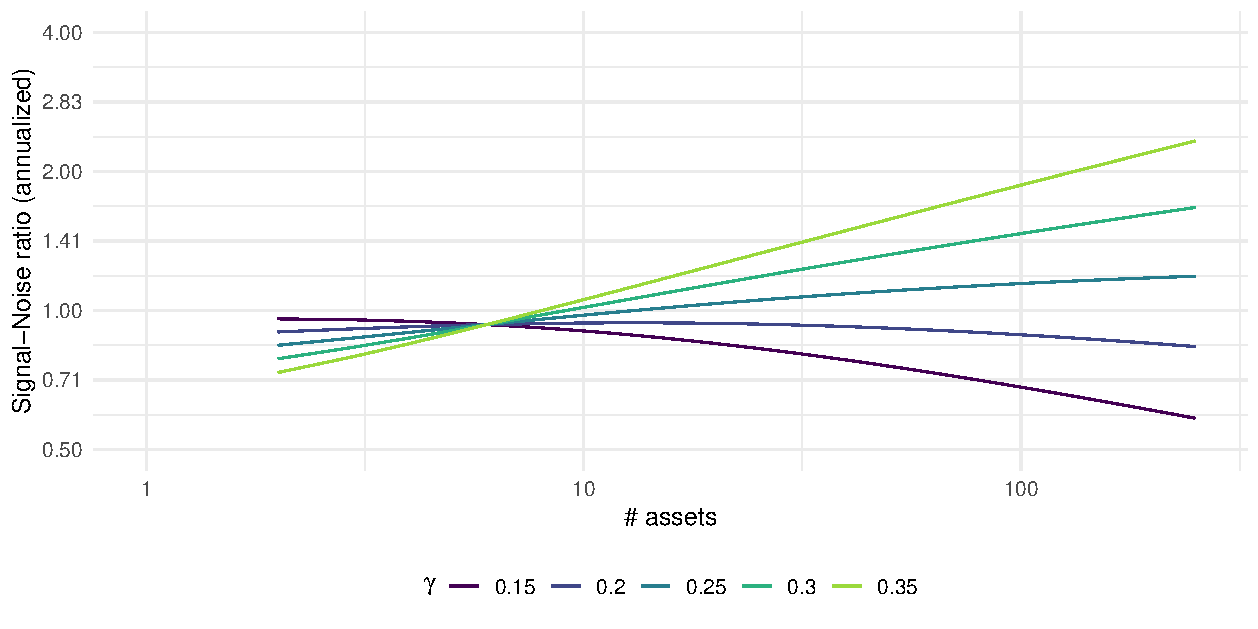
\includegraphics[width=0.99\textwidth,height=0.495\textwidth]{figure/qboundgrow_bound-1} \caption[The upper bound of \theoremref{qual_bound} is plotted versus \nlatf for different scaling laws.]{The upper bound of \theoremref{qual_bound} is plotted versus \nlatf for different scaling laws.}\label{fig:grow_bound}
\end{figure}

\end{knitrout}

The decreasing upper bound with respect to growing universe size
is illustrated in \figref{grow_bound}. Under the assumption
$\psnropt = \psnr[0]\nlatf^{\gamma}$, the upper bound
of \theoremref{qual_bound} is plotted versus \nlatf for 
different values of $\gamma$. 
The value of
$\psnr[0]$ is set so that 
$\psnropt=1.25\yrtomhalf$ when 
$\nlatf=6$.
For $\gamma < \oneby{4}$, one sees a local maximum in 
the upper bound as \nlatf increases, a behavior not seen for
$\gamma > \oneby{4}$, where the bound on \txtQual
grows with \nlatf. 


%$\psnropt$ and the $0.25, 0.50,$ and $0.75$ quantiles of
%$\psnropt\pql{\sportwfnc{\mreti}}$, under 
%\apxref{qual_dist}, are plotted versus \nlatf.
%The panels represent $\gamma$ values of
%$sort(pgammas)[1:(length(pgammas)-1)],$ and 
%$sort(pgammas)[length(pgammas)]$.
%The value of
%$\psnr[0]$ is set so that 
%$\psnropt=sqrt(ope)*zeta.s\yrtomhalf$ when 
%$\nlatf=n.stok$.
%For $\gamma < 0.25$, one sees a local maximum in 
%achieved \txtSR as \nlatf increases, a behavior not seen for
%$\gamma > 0.25$, where achieved \txtSR grows with \nlatf. 
%For the case of `slow growth' of \psnropt, the diversification 
%benefit is not seen by the sample \txtMP, rather its practical
%utility \emph{decreases} because the haircut outpaces the growth
%of \psnropt. As a practical matter, this may explain why the
%\txtMP is typically applied to small asset universes.



This relationship between \txtQual and \nlatf for different
values of $\gamma$ appears not just in the upper bound of
\theoremref{qual_bound}, but apparently also for most quantiles
of the distribution given by \apxref{qual_dist}, as
%This loss in value with respect to growing universe size is
illustrated in \figref{grow_sqrt}. Again assuming
$\psnropt = \psnr[0]\nlatf^{\gamma}$, lines of 
$\psnropt$ and the $0.25, 0.50,$ and $0.75$ quantiles of
$\psnropt\pql{\sportwfnc{\mreti}}$, under 
\apxref{qual_dist}, are plotted versus \nlatf.
The panels represent $\gamma$ values of
$0.15, 0.2, 0.25, 0.3,$ and 
$0.35$.
Again, the value of
$\psnr[0]$ is set so that 
$\psnropt=1.25\yrtomhalf$ when 
$\nlatf=6$.
For $\gamma < \oneby{4}$, one sees a local maximum in 
\txtQual as \nlatf increases, a behavior not seen for
$\gamma > \oneby{4}$, where quantiles of \txtQual grow with \nlatf. 
For the case of `slow growth' of \psnropt, the diversification 
benefit is not seen by the sample \txtMP, rather its practical
utility \emph{decreases} because the estimation error 
outpaces the growth of \psnropt. 

%Via the equivalence in \eqnref{sufficient_growth}, for the 
%bound \qbnd to be growing with respect to \nlatf, it suffices
%to establish that 
%$\half \le \wrapParens{\nlatf-1}\dbyd{\log\psnrsqopt}{\nlatf}$.
%From \eqnref{capm_zetas}, we have
%\begin{equation*}
%\begin{split}
%\half\dbyd{\log\psnrsqopt}{\nlatf} 
%&= 
%\frac{\trAB{\vect{\alpha}}{\dbyd{\vect{\alpha}}{\nlatf}} + 
%\wrapParens{\frac{\sigma_m}{\sigma}}^2 \wrapBracks{
 %\trAB{\vect{\beta}}{\dbyd{\vect{\beta}}{\nlatf}}\gram{\vect{\alpha}}
%+ \trAB{\vect{\alpha}}{\dbyd{\vect{\alpha}}{\nlatf}}\gram{\vect{\beta}}
%- \trAB{\vect{\alpha}}{\vect{\beta}}\wrapParens{
  %\trAB{\vect{\alpha}}{\dbyd{\vect{\beta}}{\nlatf}} + 
  %\trAB{\vect{\beta}}{\dbyd{\vect{\alpha}}{\nlatf}}}}}{%
%\gram{\vect{\alpha}} +
%\wrapParens{\frac{\sigma_m}{\sigma}}^2 \wrapBracks{%
%\gram{\vect{\beta}}\gram{\vect{\alpha}} -
%\wrapParens{\trAB{\vect{\alpha}}{\vect{\beta}}}^2}}
%+ \frac{\sigma_m^2 \trAB{\vect{\beta}}{\dbyd{\vect{\beta}}{\nlatf}}}{%
%\sigma^2 + \sigma_m^2\gram{\vect{\beta}}}.
%\end{split}
%\end{equation*}
%2FIX: where you going with this?
%These plots are built using \apxref{hcut_apx} ...

\subsection{Diversification under CAPM}%FOLDUP

It is not clear how \psnropt `should' scale with \nlatf. It is
easy to construct a model under which \psnropt scales as
$\nlatf^{\half}$: assume all assets have independent returns with
the same \txtSNR. It is also easy to accidentally construct 
a model under which \psnropt ultimately scales 
as $\nlatf^{\epsilon}$ for small $\epsilon$, as done here.
Suppose the \kth{i} asset has expected return
$\alpha_i$, exposure $\beta_i$ to `the market', and volatility
$\sigma$. Assume the market return is zero mean with volatility
$\sigma_m$. Then the squared \txtSNR is
\begin{align}
\nonumber
\psnrsqopt 
&= 
\frac{\gram{\vect{\alpha}} +
\wrapParens{\frac{\sigma_m}{\sigma}}^2 \wrapBracks{%
\gram{\vect{\beta}}\gram{\vect{\alpha}} -
\wrapParens{\trAB{\vect{\alpha}}{\vect{\beta}}}^2}}{\sigma^2 +
\sigma_m^2\gram{\vect{\beta}}},&\\
&= 
\frac{\gram{\vect{\alpha}}}{\sigma^2}
\frac{\sigma^2 + \sigma_m^2 \gram{\vect{\beta}} \fsin[2]{\psi}}{%
\sigma^2 + \sigma_m^2\gram{\vect{\beta}}},&
\label{eqn:capm_zetas}
\end{align}
where $\psi$ is the angle between the vectors \vect{\alpha}
and \vect{\beta}.
Depending on how the sine of $\psi$ grows with universe size, 
one observes different scaling of \psnropt with respect to \nlatf. When
the assets all have the same alpha and beta, \ie
$\vect{\alpha} = \alpha\vone$ and $\vect{\beta} = \beta\vone$,
the sine is identically zero, and 
$\psnropt = \sqrt{\fraccp{\nlatf\alpha^2}{\sigma^2 + \nlatf\sigma_m^2\beta^2}}
< \alpha\beta^{-1}\sigma_m^{-1}$. Thus 
\psnropt asymptotically scales slower than $\nlatf^{\epsilon}$
for all $\epsilon > 0$.

On the other hand, when the sine is
one, \ie when \vect{\alpha} is orthogonal to \vect{\beta},
$\psnropt = \sqrt{\gram{\vect{\alpha}}} \sigma^{-1}$, which
grows however the assets are ordered, presumably on the
order of $\nlatf^{\half}$. Thus under a CAPM model, the
growth of \psnropt depends on the `alignment' of the
vectors \vect{\alpha} and \vect{\beta}.
%UNFOLD

%UNFOLD

%%%%%%%%%%%%%%%%%%%%%%%%%%%%%%%%%%%%%%%%%%%%%%%%%%%%%%%%%%%%%%%%%%%%%%%%
\section{Generalizations}%FOLDUP

\label{sec:generalizations}

\theoremref{qual_bound} is somewhat lacking because it ignores conditioning
information which may affect the distribution of future returns, and which
may inform the portfolio manager. Few active managers, it is presumed,
are holding the unconditional \txtMP based on in-sample data. What is sought
is a more general theorem that allows more elaborate models of returns,
and more elaborate, parametrized, trading schemes, with \psnropt redefined 
as the maximal portfolio \txtQual over the trading schemes, and \nlatf
redefined as the `degrees of freedom', perhaps the rank of some derivative
at the optimal parameter, say. Towards that goal, a few generalizations can
easily be made.

\subsection{Conditional portfolio \txtQual}%FOLDUP
\label{subsec:cond_portfolio_qual}

The model of stationary mean returns is generalized by one where
the expected return of the assets is linear in some state
variables, or `features', \vfact[i], observed prior to the investment
decision.  \cite{pav_the_book,connor1997,herold2004TAA} That
is, one observes the \nfac-vector $\vfact[i]$ at some time prior to 
when the investment decision is required to capture \vreti[i+1]. 
The general model is now
\begin{align}
\label{eqn:cond_model_IV}
\Econd{\vreti[i+1]}{\vfact[i]} &=
\pRegco \vfact[i], &
\Varcond{\vreti[i+1]}{\vfact[i]} &=
\pvsig,
\end{align}
where \pRegco is some \bby{\nlatf}{\nfac} matrix. 

Here we bound the \txtQual of portfolios which are
linear in the features \vfact[i]. That is, the portfolio
manager allocates their assets proportional to
$\sportW\vfact[i]$ for some matrix $\sportW$.

Using the law of iterated expectations, the unconditional
expected value of the returns of the portfolio is
\begin{equation*}
\E{\Econd{\trAB{\wrapParens{\sportW\vfact[i]}}{\vreti[i+1]}}{\vfact[i]}}
= \trace{\tr{\sportW}\pRegco\E{\ogram{\vfact[i]}}}
= \trace{\tr{\sportW}\pRegco\pfacsig},
\end{equation*}
by definition of \pfacsig as the second moment of \vfact[i].

Unfortunately the unconditional variance will, in general,
involve a term quadratic in the expectation. However, it
can easily be shown that the unconditional \emph{expected} 
variance of the portfolio's returns is
\begin{equation*}
\E{\qform{\pvsig}{\wrapParens{\sportW\vfact[i]}}} =
\trace{\qform{\pvsig}{\sportW}\pfacsig}.
\end{equation*}
We can then redefine\footnote{If an analysis of the conditional expected
return divided by risk is required, it is possible one could define
\pQl{\cdot} as the expected return divided by square root of the unconditional
second moment. The \txtQual would then be $\ftan{\farcsin{\pQl{\cdot}}}$.
One could possibly find a \txtCR bound on the expected value of this \pQl{\cdot}.
This `Pillai-Bartlett' form of \pQl{\cdot} is likely unrequired for low frequency
settings.} the \txtQual of the portfolio as the
unconditional mean divided by the unconditional expected risk:
\begin{equation}
\pQl{\sportW}\defeq\frac{\trace{\tr{\sportW}\pRegco\pfacsig}}{%
\sqrt{\trace{\qform{\pvsig}{\sportW}\pfacsig}}}.
\end{equation}
When \vfact[i] is a deterministic scalar constant, 
this coincides with the `usual' definition of \txtQual as being 
like a \txtSR. However, except possibly for an intercept term, one
expects \vfact[i] to be random, or at least out of the control of
the portfolio manager.

Once again, a risk transform can be injected to express
portfolio optimization as an estimation problem on a sphere:
\begin{equation}
\begin{split}
\pQl{\sportW}
&=\frac{\trace{\trAB{%
\wrapParens{\trchol{\pvsig}\sportW\chol{\pfacsig}}}{%
\wrapParens{\ichol{\pvsig}\pRegco\chol{\pfacsig}}}{%
}}}{%
\sqrt{\trace{
\gram{\wrapParens{\trchol{\pvsig}\sportW\chol{\pfacsig}}}}}},\\
&=
\frac{\trAB{\fvec{\trchol{\pvsig}\sportW\chol{\pfacsig}}}{%
\fvec{\ichol{\pvsig}\pRegco\chol{\pfacsig}}}}{%
\sqrt{\gram{\fvec{\trchol{\pvsig}\sportW\chol{\pfacsig}}}}}.
\end{split}
\end{equation}
This function is maximized by taking
\begin{equation}
\sportW = \pportWopt \defeq \minv{\pvsig}{\pRegco},
\end{equation}
which has \txtQual
\begin{equation}
\psnropt\defeq\pQl{\pportWopt} =
\sqrt{\trace{\qiform{\pvsig}{\pRegco}\pfacsig}}.
\end{equation}
The square of this quantity, \psnrsqopt, 
is the `population analogue' of the Hotelling-Lawley trace. \cite{Rencher2002,Muller1984143}

Again we can write
\begin{equation*}
\frac{\pQl{\sportW}}{\psnropt} = 
\trAB{\fnorm{\fvec{\trchol{\pvsig}\sportW\chol{\pfacsig}}}}{%
\fnorm{\fvec{\ichol{\pvsig}\pRegco\chol{\pfacsig}}}}.
\end{equation*}
Thus finding a `good' \sportW becomes an estimation problem on the
sphere \sphere{\nfac\nlatf - 1}. An analogue
to \theoremref{qual_bound} can be proved with $\nfac\nlatf$ replacing
$\nlatf$, by assuming a particular form to the likelihood. We must
generalize the assumption of Directional Independence, after which
the theorem proceeds easily.

\begin{assumption}[Conditional Directional Independence]%FOLDUP
Assume that
\begin{equation}
\label{eqn:sane_estimator_cond}
\E{\fnorm{\fvec{\trchol{\pvsig}\sportWfnc{\mreti,\mfact}}}} = 
\cfnc{\psnrsqopt} \fnorm{\fvec{\trchol{\pvsig}\pportWopt\chol{\pfacsig}}}
+ \Bterm,
\end{equation}
where \Bterm is the bias term, orthogonal to 
\fnorm{\fvec{\trchol{\pvsig}\pportWopt\chol{\pfacsig}}}.
\end{assumption}%UNFOLD

\begin{theorem}%FOLDUP
\label{theorem:qual_bound_two}
Let one element of \vfact[i] be a deterministic $1$. Suppose the
vector of the remaining $\nfac-1$ elements of \vfact[i] stacked 
on top of \vreti[i+1] are multivariate Gaussian.  Let \mreti, 
\mfact be \bby{\ssiz}{\nlatf} and \bby{\ssiz}{\nfac} matrices
of \iid observations of the features and returns.
Let \sportWfnc{\mreti,\mfact} be an estimator 
%based on 
%\ssiz \iid observations of multivariate Gaussian returns, \mreti, 
%and multivariate Gaussian features, \mfact, with one column of \mfact
%an intercept term, 
satisfying the assumptions of
Conditional Directional Independence and Residual Independence. Then
\begin{equation}
\E{\pQl{\sportWfnc{\mreti,\mfact}}} 
\le \frac{\sqrt{\ssiz}\psnrsqopt}{\sqrt{\nfac\nlatf - 1 + \ssiz\psnrsqopt}}.
\end{equation}
\end{theorem}%UNFOLD
\begin{proof}%FOLDUP

We can proceed as in \secref{portfolio_qual}. Let \mreti be the 
\bby{\ssiz}{\nlatf} matrix of portfolio returns, and let 
\mfact be the corresponding \bby{\ssiz}{\nfac} matrix of features.
View the portfolio coefficient \sportW as an estimator, a function of
the random data, \ie \sportWfnc{\mreti,\mfact}.
%Assume
%Directional Independence, with \eqnref{sane_estimator}
%becoming
%\begin{equation}
%\E{\fnorm{\trchol{\pvsig}\sportWfnc{\mreti,\mfact}}} = 
%\cfnc{\psnrsqopt} \fnorm{\trchol{\pvsig}\pportWopt\chol{\pfacsig}}
%+ \Bterm.
%\end{equation}
Define
\begin{equation}
\prskMtx\defeq{\ichol{\pvsig}\pRegco\chol{\pfacsig}}.
\end{equation}
Then 
\begin{equation*}
\psnrsqopt = \trace{\gramprskMtx}.
\end{equation*}

We get, analogously to \eqnref{crb_one},
\begin{equation}
\oneby{\ssiz}\trace{\qoform{\iFishI[\fvec{\prskMtx}]}{\Drv}}
\le 1 - \csqfnc{\trace{\gramprskMtx}},
\end{equation}
where
\begin{equation}
\Drv\defeq
{\dbyd{\cfnc{\trace{\gramprskMtx}}\frac{\prskMtx}{\sqrt{\trace{\gramprskMtx}}}}{\fvec{\prskMtx}}}.
\end{equation}

Without loss of generality, we assume it is the first element
of \vfact[i] that is a deterministic $1$. Then, the log likelihood of 
the vector of $\vfact[i]$ stacked on top of $\vreti[i+1]$
is: \cite{pav2013markowitz}
\begin{equation}
\label{eqn:cond_llik_one}
\log \FOOlik{}{\pvsm}{\twobyone{\vfact[i]}{\vreti[i+1]}} = 
  c_{\nfac+\nlatf} 
- \half \logdet{\pvsm} 
- \half \trace{\minv{\pvsm}\ogram{\twobyone{\vfact[i]}{\vreti[i+1]}}},
\end{equation}
where \pvsm is the second moment matrix:
\begin{equation}
\pvsm \defeq \E{\ogram{\twobyone{\vfact[i]}{\vreti[i+1]}}}
= \twobytwo{\pfacsig}{\pfacsig\tr{\pRegco}}{\pRegco\pfacsig}{\pvsig +
\qoform{\pfacsig}{\pRegco}}.
%\qoform{\pfaccov}{\pRegco}}}.
\end{equation}
The inverse of \pvsm has the following, somewhat surprising, form \cite{pav2013markowitz}:
\begin{equation}
\minv{\pvsm} 
= \twobytwo{\minv{\pfacsig} +
\qiform{\pvsig}{\pRegco}}{-\tr{\pRegco}\minv{\pvsig}}{-\minv{\pvsig}\pRegco}{\minv{\pvsig}}.
\end{equation}
A square root of this matrix (a Cholesky factor, up to permutation)
is:
\begin{equation}
\begin{split}
\minv{\pvsm} &=
\ogram{%
\twobytwo{\ichol{\pfacsig}}{-\tr{\pRegco}\ichol{\pvsig}}{\mzero}{\ichol{\pvsig}}
},\\
&= \twobytwo{\ichol{\pfacsig}}{\mzero}{\mzero}{\eye}
\ogram{%
\twobytwo{\eye}{-\prskMtxU{\trsym}}{\mzero}{\ichol{\pvsig}}}
\twobytwo{\trichol{\pfacsig}}{\mzero}{\mzero}{\eye}.
\end{split}
\end{equation}

By the block determinant formula, 
\begin{equation}
\det{\pvsm} 
= \det{\pfacsig}\det{\pvsig + \qoform{\pfacsig}{\pRegco} -
\pRegco\pfacsig\minv{\pfacsig}\pfacsig\tr{\pRegco}}
= \det{\pfacsig}\det{\pvsig}.
\end{equation}
Thus, conditional on \pfacsig and \pvsig, the negative log likelihood
takes the form:
\begin{multline}
\label{eqn:cond_llik_two}
- \log \FOOlik{}{\prskMtx, \pfacsig, \pvsig}{\twobyone{\vfact[i]}{\vreti[i+1]}} = 
- c_{\nfac+\nlatf}
+ \half \logdet{\pfacsig} 
+ \half \logdet{\pvsig}\\
+ \half \trace{
\ogram{%
\twobytwo{\eye}{-\prskMtxU{\trsym}}{\mzero}{\ichol{\pvsig}}}
\ogram{\twobyone{\trichol{\pfacsig}\vfact[i]}{\vreti[i+1]}}}.
\end{multline}
Sweeping the nuisance parameter terms into the constant, as well
as terms in the trace which are not quadratic in \prskMtx, we
have 
\begin{align}
\label{eqn:cond_llik_three}
- \log \FOOlik{}{\prskMtx, \pfacsig, \pvsig}{\twobyone{\vfact[i]}{\vreti[i+1]}}
&= - c'
+ \half \trace{\gramprskMtx 
\ogram{\wrapParens{\trichol{\pfacsig}\vfact[i]}}},&\\
&= - c'
+ \half
\tr{\fvec{\prskMtx}}\fvec{\prskMtx\trichol{\pfacsig}\ogram{\vfact[i]}\ichol{\pfacsig}}.&\\
&= - c'
+ \half
\tr{\fvec{\prskMtx}}\wrapParens{%
\wrapBracks{\trichol{\pfacsig}\ogram{\vfact[i]}\ichol{\pfacsig}}
 \kron \eye}\fvec{\prskMtx}.&
\end{align}
The Fisher Information, then, is
\begin{equation}
\FishI[\fvec{\prskMtx}] =
\E{\wrapParens{%
\wrapBracks{\trichol{\pfacsig}\ogram{\vfact[i]}\ichol{\pfacsig}}
 \kron \eye}} = \eye[\nfac\nlatf].
\end{equation}

The remainder of the proof proceeds exactly as in 
\secref{portfolio_qual}. 
\end{proof}%UNFOLD

%\begin{theorem}
%\label{theorem:qual_bound_two}
%Let \sportWfnc{\mreti,\mfact} be an estimator based on 
%\ssiz \iid observations of multivariate Gaussian returns, \mreti, 
%and multivariate Gaussian features, \mfact, with one column of \mfact
%an intercept term, satisfying the assumptions of
%directional independence and residual independence. Then
%\begin{equation}
%\E{\pQl{\sportWfnc{\mreti,\mfact}}} 
%\le \frac{\sqrt{\ssiz}\psnrsqopt}{\sqrt{\nlatf\nfac - 1 + \ssiz\psnrsqopt}}.
%\end{equation}
%\end{theorem}

%&= \E{\Cmat\scoro{\prskvec}{\FOOlik{}{\prskvec}{\mreti}}

%\begin{equation}
%\begin{split}
%\vfact[i] &\sim \normlaw{\pfacmu, \pfaccov},\\
%\condtwo{\vreti[i+1]}{\vfact[i]} &\sim \normlaw{\pRegco\vfact[i], \pvsig}.
%\end{split}
%\end{equation}
%Together the unconditional distribution is
%\begin{equation}
%\twobyone{\vfact[i]}{\vreti[i+1]} \sim
%\normlaw{\twobyone{\pfacmu}{\pRegco\pfacmu}, 
%\twobytwo{\pfaccov}{\pfaccov\tr{\pRegco}}{\pRegco\pfaccov}{\pvsig +
%\qoform{\pfaccov}{\pRegco}}}.
%\end{equation}




%In this model, the `Markowitz Coefficient' 
%$\minvAB{\pvsig}{\pRegco}$, generalizes the \txtMP as
%the coefficient of the optimal portfolio which is linear in \vfact,
%under some objective. \cite{pav2013markowitz} How should we define
%the \txtQual of the Markowitz Coefficient, and can we prove
%an analogue of \theoremref{qual_bound}?
%UNFOLD

\subsection{Subspace constraints}%FOLDUP

Consider, now, the case of conditional expectation, as presented in
\subsecref{cond_portfolio_qual}, but where the portfolio is 
constrained to be in some lower dimensional subspace. That is, by design, 
\begin{equation}
\zerJc \sportWfnc{\mreti,\mfact} = \vzero,
\end{equation}
where $\zerJc$ is a \bby{\wrapParens{\nlatf - \nlatfzer}}{\nlatf}
matrix of rank $\nlatf - \nlatfzer$, that is chosen independently
of the observations of \mreti and \mfact.
Let the rows of \zerJ span the null space of the rows of
\zerJc; that is, $\zerJc \tr{\zerJ} = \mzero$, and $\ogram{\zerJ} = \eye$.

We can simply use the results of \subsecref{cond_portfolio_qual}, but
replacing the assets with the \nlatfzer assets spanned by the rows of
\zerJ. That is, we can replace the \vreti[i+1] with $\zerJ\vreti[i+1]$,
and replace \sportWfnc{\mreti,\mfact} with
$\tr{\zerJ}\minv{\wrapParens{\ogram{\zerJ}}}\sportWfnc{\mreti,\mfact}$
to arrive at the following analogue of \theoremref{qual_bound_two}:

\begin{theorem}%FOLDUP
\label{theorem:qual_bound_three}
Let one element of \vfact[i] be a deterministic $1$. Suppose the
vector of the remaining $\nfac-1$ elements of \vfact[i] stacked 
on top of \vreti[i+1] are multivariate Gaussian.  Let \mreti, 
\mfact be \bby{\ssiz}{\nlatf} and \bby{\ssiz}{\nfac} matrices
of \iid observations of the features and returns.
Let \sportWfnc{\mreti,\mfact} be an estimator 
%based on 
%\ssiz \iid observations of multivariate Gaussian returns, \mreti, 
%and multivariate Gaussian features, \mfact, with one column of \mfact
%an intercept term, 
satisfying the assumptions of
directional independence and residual independence, with the constraint
\begin{equation}
\zerJc \sportWfnc{\mreti,\mfact} = \vzero,
\end{equation}
for \bby{\wrapParens{\nlatf - \nlatfzer}}{\nlatf} matrix \zerJc, which
is chosen independently of the observed \mreti and \mfact. 
Let the rows of \zerJ span the null space of the rows of
\zerJc. 

Then
\begin{equation}
\E{\pQl{\sportWfnc{\mreti,\mfact}}} 
\le \frac{\sqrt{\ssiz}\psnrsqoptG{\zerJ}}{\sqrt{\nfac\nlatfzer - 1 +
\ssiz\psnrsqoptG{\zerJ}}},
\end{equation}
where 
\begin{equation*}
\psnrsqoptG{\zerJ}\defeq 
\trace{\qform{\wrapProj{\pvsig}{\zerJ}}{\pRegco}\pfacsig}.
\end{equation*}
\end{theorem}%UNFOLD
%UNFOLD

\subsection{Hedging constraints}%FOLDUP

Consider, now, the case where one seeks a portfolio whose returns are
independent, in the probabilistic sense, of the returns of some 
traded instruments in the investment universe. 
Independence is a difficult property to
check or enforce; however, independence implies zero covariation, which
can be easily formulated and checked. 

Since the portfolio estimator may not deliver a perfectly
hedged portolio due to misestimation of the covariance matrix, we
will, with perfect knowledge of \pvsig, consider the \txtQual of the 
hedged part of the portfolio. The hedged
part is defined in terms of a risk projection. 
If \sportw[1] is a feasible portfolio based on the sample,
then the hedged version of this portfolio is the solution to the
optimization problem
\begin{equation}
\min_{\sportw : \hejG\pvsig\sportw = \vzero} \VAR{\trAB{\wrapParens{\sportw -
\sportw[1]}}{\vreti[i+1]}},
\end{equation}
where $\hejG$ is a \bby{\nlatfhej}{\nlatf} matrix of 
rank \nlatfhej, the rows of which we wish to `hedge out.'

Using the Lagrange multiplier technique, this can easily be found to
be solved by 
\begin{equation}
\sportw = \sportw[1] - \wrapProj{\pvsig}{\hejG}\pvsig\sportw[1].
\end{equation}
Thus we will consider the \txtQual of the portfolio estimator
\begin{equation*}
\wrapParens{\eye[\nlatf] - \wrapProj{\pvsig}{\hejG}\pvsig}\sportWfnc{\mreti,\mfact}.
\end{equation*}
Note, however, that the row rank of
$\wrapParens{\eye[\nlatf] - \wrapProj{\pvsig}{\hejG}\pvsig}$ 
is $\nlatf - \nlatfhej$.  Thus hedging is an instance of a subspace
constraint and we can apply \theoremref{qual_bound_three} outright.

\begin{theorem}%FOLDUP
\label{theorem:qual_bound_four}
Let one element of \vfact[i] be a deterministic $1$. Suppose the
vector of the remaining $\nfac-1$ elements of \vfact[i] stacked 
on top of \vreti[i+1] are multivariate Gaussian.  Let \mreti, 
\mfact be \bby{\ssiz}{\nlatf} and \bby{\ssiz}{\nfac} matrices
of \iid observations of the features and returns.
Let \sportWfnc{\mreti,\mfact} be an estimator 
%based on 
%\ssiz \iid observations of multivariate Gaussian returns, \mreti, 
%and multivariate Gaussian features, \mfact, with one column of \mfact
%an intercept term, 
satisfying the assumptions of
directional independence and residual independence. 
Let \bby{\nlatfhej}{\nlatf} matrix \hejG be chosen
independently of \mreti and \mfact. 

%2FIX: redefine Deltapsnr to not be confusing.
Define 
\begin{equation}
\Delpsnrsqopt{\eye,\hejG}
\defeq
\trace{\qiform{\svsig}{\pRegco}\pfacsig} - 
\trace{\qform{\wrapProj{\pvsig}{\hejG}}{\pRegco}\pfacsig}.
\end{equation}

Then
\begin{equation}
\E{\pQl{%
\wrapBracks{\eye[\nlatf] - \wrapProj{\pvsig}{\hejG}\pvsig}\sportWfnc{\mreti,\mfact}}} 
\le \frac{\sqrt{\ssiz}\Delpsnrsqopt{\eye,\hejG}}{\sqrt{\nfac\wrapParens{\nlatf -
\nlatfhej} - 1 + \ssiz\Delpsnrsqopt{\eye,\hejG}}}.
\end{equation}
\end{theorem}%UNFOLD

%UNFOLD

%UNFOLD

%%%%%%%%%%%%%%%%%%%%%%%%%%%%%%%%%%%%%%%%%%%%%%%%%%%%%%%%%%%%%%%%%%%%%%%%
\section{Examples}%FOLDUP

\subsection{The equal weight puzzle}%FOLDUP


\theoremref{qual_bound} can help us make sense of puzzling findings
in the literature. For example, in the ``$1/N$'' paper, DeMiguel \etal
find that the equal-weighting portfolio outperforms, in terms of out-of-sample
\txtSR (and other measures), the \txtMP and numerous other portfolio
estimators.  \cite{demiguel2009optimal}
This finding is supported on a number of real world data
sets, and a few synthetic ones. One data set used was the returns of
the 10 industry portfolios and the US equity market portfolio, computed
by Ken French. 
% 2FIX: add citation to data.

The monthly returns, from 1927-01-01 to 
2020-12-01, for these 10 
assets were downloaded
from Kenneth French's data library.  \cite{French10Port}
%from \emph{Quandl}.  \cite{Quandl}
The \txtSR of the equal weighted portfolio on the %10
assets, over the 1128 months, is around 
$0.67\yrtomhalf$. The \txtSR of the sample \txtMP over
the 10 assets over the same period is around
$0.86\yrtomhalf$.  
Now consider a portfolio estimator
given 5 years of observations, as in 
DeMiguel \etal \cite{demiguel2009optimal}, assuming 
$\psnropt=0.86\yrtomhalf$.
The bound on expected value of \pql{\sportwfnc{\mreti}} from \theoremref{qual_bound} is only $0.46\yrtomhalf$.  
%Under \apxref{qual_dist}, the probability that \pql{\sportwfnc{\mreti}} exceeds $sr1$sr\yrtomhalf$ in this case is only $dfp$. 
It is not surprising that DeMiguel \etal drew
the conclusions they did, nor that they would be refuted
by looking at a longer sample, as by Kritzman \etal \cite{defoopt2010}



One could also use \theoremref{qual_bound_four} here. However,
the upper bound of that theorem is non-negative, and zero only
if the quantity \Delpsnrsqopt{\eye,\hejG} is zero.  This is a
statement regarding unknown population parameters, but we can
perform inference on this quantity. For example, based on the
1128 months of data on these 
10, the 95\% confidence interval on
\Delpsnrsqopt{\eye,\hejG}, where \hejG is the \bby{1}{10}
matrix of all ones, is
$\asrowvec{0.04, 0.45}\yrto{-1}$, under the assumption of
Gaussian returns.  

%One could view the touted superiority of the equal weight portfolio
%over \eg the \txtMP as a veiled claim that there is a single
%discount factor that rules all asset returns. As stated, this claim
%is clearly absurd, since \eg an equal weight portfolio on both pairs
%of leveraged ETFs is clearly inferior to a portfolio equal weight \emph{short}
%both pairs.  \cite{zhang2010path}

%This highlights
%the fact that the putative superiority of the equal weight portfolio
%may be based on two due less to deficiencies in \eg the \txtMP, and more to
%the 

%The analysis presented here is likely to be optimistic when one
%considers the \emph{spanning} aspect of this problem.  
%\cite{giri1964likelihood,HKspan1987,KanZhou2012} That is, the
%total effect size beyond the equal weighting subspace may be
%very small. A `proper' analysis would take into account the
%difference in effect sizes and differences in universe size. 
%However, the spanning analogue of \theoremref{qual_bound}
%has not yet been established.

%% 2FIX: talk about the spanning statistics here. is there
%% any effect to exploit?
%The result is dKRS or
%dUNB or
%dMLE.
%the upper bound is asqb.
%Show it as:
%dsr2
%or cis: myci.

%UNFOLD

\subsection{Empirical diversification in the S\&P 100}%FOLDUP



To check how \psnropt \emph{might} scale with \nlatf, the weekly
log returns of the adjusted close prices of the stocks in the 
S\&P 100 Index, as of March 21, 2014, were downloaded 
from \emph{Quandl}.  \cite{Quandl} 
Adjustments for splits and
dividends were made in some unspecified way by the upstream source
of the data, Yahoo Finance. Stocks without a full 5 years of history
were discarded, leaving 96 stocks. 
Note that selection based on membership in the index at the end of the 
period adds no small amount of selection bias, which we shall ignore 
here.

Based on the weekly returns from 2009-03-27 to 2014-04-04,
estimates of \psnropt were computed, using the `KRS' estimator.
\cite{kubokawa1993estimation,pav_the_book} 
This was performed on the first \nlatf assets, with \nlatf ranging from 
$1$ to $96$.  The estimate of \psnropt versus \nlatf
is plotted in \figref{sp100_grow}, with assets added in alphabetical order.
Because Apple appears at the beginning of this list, it appears that
\psnropt starts reasonably large, but then actually \emph{decreases}
when adding assets. This is an artifact of the estimator, since the true
\psnropt can only increase when adding assets. 

\begin{knitrout}\small
\definecolor{shadecolor}{rgb}{0.969, 0.969, 0.969}\color{fgcolor}\begin{figure}[h]
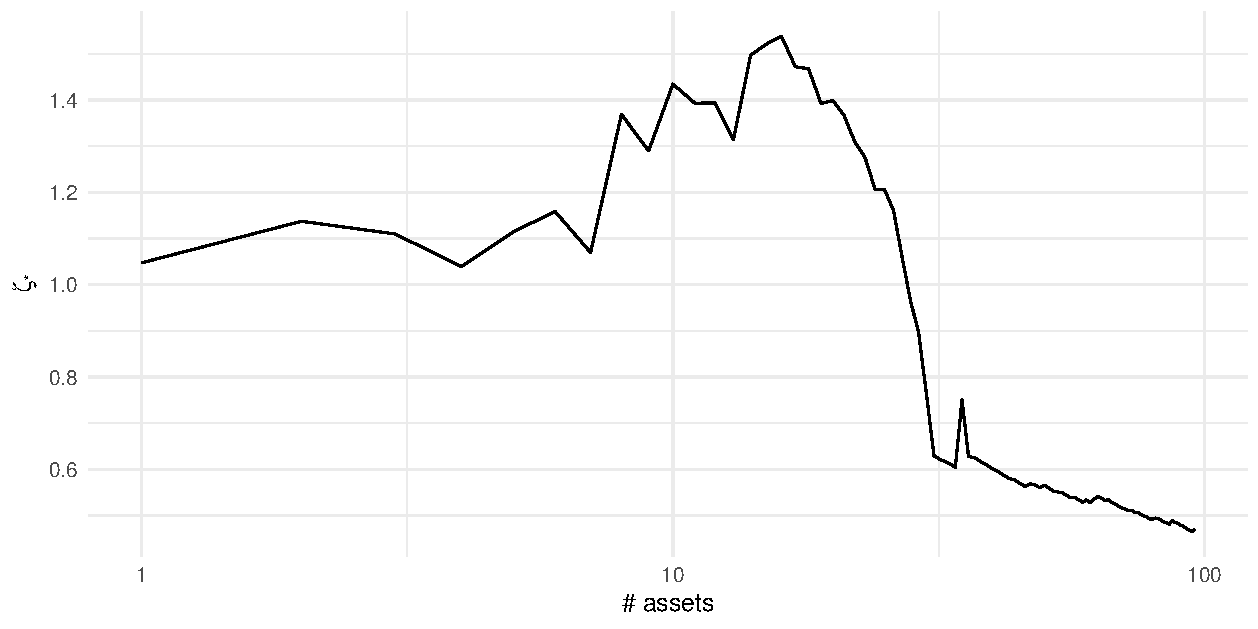
\includegraphics[width=0.99\textwidth,height=0.495\textwidth]{figure/qboundsp100_grow-1} \caption[Growth of estimated \psnropt versus \nlatf for the S\&P 100 Index names, in alphabetical order, showing the `Apple effect.']{Growth of estimated \psnropt versus \nlatf for the S\&P 100 Index names, in alphabetical order, showing the `Apple effect.'}\label{fig:sp100_grow}
\end{figure}

\end{knitrout}

%<<'sp100_mid',eval=TRUE,cache=FALSE,fig.width=5.75,fig.height=3.75,dpi=450,fig.cap=paste0("Growth of estimated \\psnropt versus \\nlatf for the S\\&P 100 Index names."),eval.after='fig.cap'>>= 

%foo.df <- data.frame(df=(1:length(KRSs)),KRS=KRSs,
		%MLE=MLEs,meanKRS=rowMeans(buncho.KRSs))

%require(ggplot2)
%ph <- ggplot(data=foo.df,aes(x=df,y=meanKRS))
%ph <- ph + geom_line()
%ph <- ph + labs(x="# assets",
								%y=expression(zeta["*"]))
%ph <- ph + scale_x_log10()
%ph <- ph + scale_y_log10()
%print(ph)

%@

Since the ordering of assets here is arbitrary, the experiment was repeated
1000 times, with the stocks randomly permuted, and 
\psnropt estimated as a function of \nlatf. Boxplots, over the
1000 simulations, of the KRS statistic versus
\nlatf are given in \figref{sp100_box}. There is effectively no 
diversification benefit observed here beyond the mean effect, which is
equivalent to holding an equal weight portfolio. Given the 
conditions under which \txtQual grows with \nlatf outlined in 
\secref{diversification}, one expects poor performance of 
directionally independent portfolio estimators
over even a small subset of the S\&P 100.

\begin{knitrout}\small
\definecolor{shadecolor}{rgb}{0.969, 0.969, 0.969}\color{fgcolor}\begin{figure}[h]
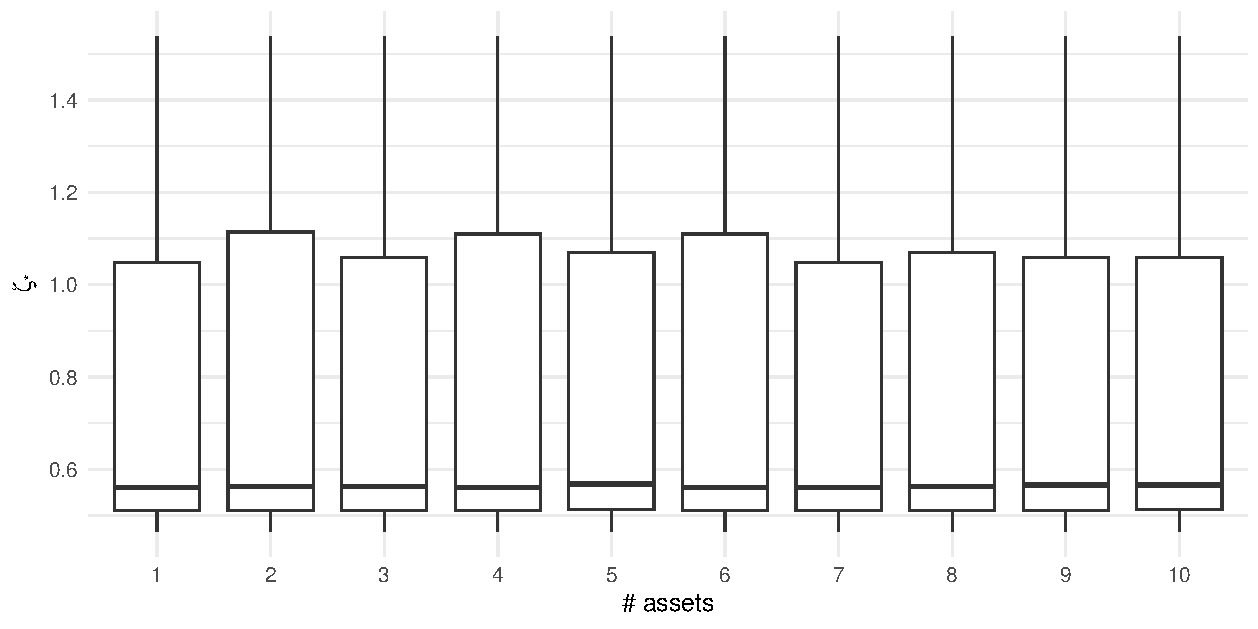
\includegraphics[width=0.99\textwidth,height=0.495\textwidth]{figure/qboundsp100_box-1} \caption[Growth of estimated \psnropt versus \nlatf for the S\&P 100 Index names is shown over 1000 permutations of the stocks, showing that there is effectively \emph{no} diversification benefit here beyond an equal weight portfolio]{Growth of estimated \psnropt versus \nlatf for the S\&P 100 Index names is shown over 1000 permutations of the stocks, showing that there is effectively \emph{no} diversification benefit here beyond an equal weight portfolio.}\label{fig:sp100_box}
\end{figure}

\end{knitrout}
%UNFOLD
%UNFOLD

%%%%%%%%%%%%%%%%%%%%%%%%%%%%%%%%%%%%%%%%%%%%%%%%%%%%%%%%%%%%%%%%%%%%%%%%
\section{Discussion}%FOLDUP

Care should be taken in the interpretation of \theoremref{qual_bound},
or its generalizations from \secref{generalizations}.
It does not claim that the sample \txtMP is somehow `optimal,' nor
does it make comparative claims about different portfolio estimators
when presented with the same data.
The theorem does not imply that somehow `overfitting' to the observed
data can be mitigated by selecting a less desireable portfolio. 
It does not claim that sample estimates of the \txtQual of a portfolio
are useless.  It is trivially
the case, for example, that if $\pql{\sportw[1]} > \pql{\sportw[2]}$, then,
with probability greater than half, 
$\trAB{\sportw[1]}{\svmu} / \sqrt{\qform{\svsig}{\sportw[1]}} > 
\trAB{\sportw[2]}{\svmu} / \sqrt{\qform{\svsig}{\sportw[2]}}$, where
the probability is over draws of \svmu and \svsig.
The theorem does not claim that the expected
\txtQual of a portfolio estimator is negative. (Indeed, it can not,
since the portfolio estimator which generates a random portfolio, 
ignoring the data, has zero expected \txtQual). 
The theorem makes no claims (\eg providing a Bayesian posterior) about 
any particular portfolio based on a single sample of the data: it is
a statement about the expectation of the \emph{estimator} under replication 
of draws of the sample.

One should recognize, moreover, there are situations where the assumptions
of the theorem are violated. For example, in some cases a prior 
bias for positive expected returns, \ie $\pvmu \ge 0$, is warranted,
and thus a portfolio estimator with a long bias is chosen.
This can happen when the underlying assets are equities, and
the eligible universe is based on some minimum longevity, as this 
introduces a `good' survivorship bias: 
companies with negative expected return should founder and perish, 
leaving behind those with more positive $\pmu$. Effectively this
acts to boost \ssiz somewhat, although the effect is likely small.

There are other reasonable portfolio estimators which violate the 
assumption of Directional Independence. For example, an estimator
which performs some dimensionality reduction based on the observed
data, \mreti and \mfact will not be covered by 
\theoremref{qual_bound_three} since the subspace is chosen based
on the sample. However, it might not be covered by 
\theoremref{qual_bound_two} because the expected \txtQual might
depend on how \pRegco aligns with the leading eigenvectors of
\pvsig, say.

\subsection{Future work}%FOLDUP

These findings perhaps raise more questions than they answer:
%This work leaves unanswered a number of interesting questions:
\begin{compactenum}
\item Foremost, the bounds of 
\theoremref{qual_bound} and \theoremref{qual_bound_two}
depend on the unknown
quantity, \psnrsqopt. How can we perform inference, 
Frequentist or Bayesian, on \pql{\sportwopt}, where \sportwopt is the \txtMP, 
given the observed information (\viz \svmu and \svsig)? This
is a problem of enormous practical concern to hundreds of
quantitative portfolio managers.

Contrast inference on the portfolio \txtQual with inference
on the population \txtSNR: under Gaussian returns, the
distribution of \ssrsqopt in terms of \ssiz, \nlatf and \psnrsqopt
is known. \cite[Theorem 5.2.2]{anderson2003introduction}
Thus, for example, the quantity
$\wrapParens{1 - \fracc{\nlatf}{\ssiz}}\ssrsqopt - \fracc{\nlatf}{\ssiz}$
is an unbiased estimator for \psnrsqopt, \etc 
Performing inverence on \pql{\sportwopt} is tricky because \psnrsqopt
is unknown and the error $\sportwopt - \pportwopt$ is likely
not independent of the error in the estimate \ssropt.

It may be the case, however, that inference on the portfolio
\txtQual qualifies as an `impossible' estimation-after-selection
problem. \cite{leeb2006}
\item While \theoremref{qual_bound} requires Gaussian returns, 
one expects that the result holds for returns distributions whose 
likelihood is ``more concave'' than the Gaussian at the MLE.
Exact conditions for this to hold should be established.
%\item How is \txtQual affected by the imposition of hedging and
%other constraints?  \cite{pav2013markowitz} Does dimensionality
%reduction modify the `degrees of freedom' in the straightforward
%way? Is there an analogue of the bound for portfolio
%spanning?  \cite{giri1964likelihood,HKspan1987,KanZhou2012}
%That is, can we find a bound on $\E{\pql{\sportw[2]} - \pql{\sportw[1]}}$,
%where \sportw[1] is a portfolio on a subspace of the assets over
%which \sportw[2] is selected, with the bound depending on the 
%spanning parameter, $\psnrsqoptG{2} - \psnrsqoptG{1}$?
\item \theoremref{qual_bound_two} applies to the case of 
trading strategies where the portfolio is linear in the 
observable features, \vfact[i]. 
Can it be used as an approximate bound for trading
strategies which are nonlinear, complex functions of the features?
\item What can be said about scaling of \psnropt with respect to
\nlatf for different models of market returns? Can one establish
sane sufficient conditions for which \psnropt grows slower than
$\nlatf^{\oneby{4}}$? What is the analogue of \eqnref{capm_zetas}
for a multi-factor model of returns?
%\item Can we find a lower bound, or a non-trivial upper bound on the 
%variance of $\pql{\sportwfnc{\mreti}}$? Together these could be used
%to give guarantees about the quantiles of \pql{\sportwfnc{\mreti}}.
%A lower bound on the variance can likely be had via a result of
%Kakarala and Watson. \cite{ANZS:ANZS253} Together with Cantelli's
%Inequality, these would give rough (perhaps useless) upper bounds
%on the 
%\kth{\qlev} quantile of portfolio \txtQual, for $\half < \qlev < 1$.
%\item The simulations of \secref{apx_distribution} should
%be repeated with different choices of \ssiz, \nlatf, and \psnropt.
\item How tight is the bound of \theoremref{qual_bound}, and can 
it be much improved by directly analyzing the differential
inequality of \eqnref{crb_three}, rather than discarding
the derivative term? Or perhaps the bound can be improved by using
an `intrinsic' \txtCR bound.  \cite{DBLP:conf/icassp/XavierB05}
%\item How good is \apxref{qual_dist}? Can we find the expected
%value of the distribution in \apxref{qual_dist}, and what is the
%gap between it and the bound of \theoremref{qual_bound}?
%Can we find the \emph{exact} distribution of \txtQual of the 
%sample \txtMP under Gaussian returns, 
%perhaps leveraging the work of Bodnar and Okhrin,
%or of Britton-Jones.  \cite{SJOS:SJOS729, BrittenJones1999}
\item Can the assumption of Directional Independence be weakened?
Can the \theoremref{qual_bound_two} be generalized to deal with omitted 
variable bias in \vfact[i]?  
\item The analysis of \txtQual ignores the `risk-free' or `disastrous'
rate of return, and all trading costs. Can the expected bounds
be generalized to include these costs?
\end{compactenum}
%UNFOLD
%UNFOLD

%%%%%%%%%%%%%%%%%%%%%%%%%%%%%%%%%%%%%%%%%%%%%%%%%%%%%%%%%%%%%%%%%%%%%%%%
% bibliography%FOLDUP
%\nocite{markowitz1952portfolio,markowitz1999early,markowitz2012foundations}
%\bibliographystyle{jss}
%\bibliographystyle{siam}
%\bibliographystyle{ieeetr}
%\bibliographystyle{plainnat}
\bibliographystyle{apacite}
%\bibliographystyle{acm}
\bibliography{SharpeR,rauto}
%UNFOLD

%%%%%%%%%%%%%%%%%%%%%%%%%%%%%%%%%%%%%%%%%%%%%%%%%%%%%%%%%%%%%%%%%%%%%%%%
\appendix%FOLDUP

\section{Miscellaneous Proofs}%FOLDUP
\label{sec:misc_proofs}

%UNFOLD

\section{Declaration of Interests}

The authors report no conflicts of interest.
The authors alone are responsible for the content and writing of the paper.

%UNFOLD

%It is trivial to show that for random variable $\vect{y}$,
%\E{\gram{\wrapParens{\vect{y} - \vect{z}}}} is minimized by
%$\vect{z} = \E{\vect{y}}$. Moreover, we have
%\begin{equation*}
%\begin{split}
%\E{\gram{\wrapParens{\vect{y} - \E{\vect{y}}}}} 
%&= \E{\trace{\gram{\wrapParens{\vect{y} - \E{\vect{y}}}}}},\\
%&= \trace{\E{\ogram{\wrapParens{\vect{y} - \E{\vect{y}}}}}},\\
%&= \trace{\VAR{\vect{y}}}.
%\end{split}
%\end{equation*}
%Thus, if we take the expectation
%of \eqnref{cos_law_form}, we can then bound the left hand
%side from below by the trace of the variance:
%\begin{equation}
%\begin{split}
%\trace{\VAR{\fnorm{\trchol{\pvsig}\sportwfnc{\mreti}}}} 
%&\le 2 - 2 \E{\frac{\pql{\sportwfnc{\mreti}}}{\psnropt}},\\
%&= 2 \wrapParens{1 -
%\trAB{{\E{\fnorm{\trchol{\pvsig}\sportwfnc{\mreti}}}}}{%
%\fnorm{\trchol{\pvsig}\pportwopt}}}.
%\label{eqn:var_bounds}
%\end{split}
%\end{equation}
%By bounding the variance via a \txtCR bound, we can find an
%upper bound on the expected value of \pql{\sportw}.

%Using the quadratic formula, we have
%\begin{equation}
%\cfnc{\gramprskvec} \le \frac{-\ssiz\gramprskvec +
%\sqrt{\ssiz^2\wrapParens{\gramprskvec}^2 + 2
%\ssiz\gramprskvec\wrapParens{\nlatf-1}}}{\nlatf - 1}.
%\end{equation}
%For $\ssiz\gramprskvec$ large, we have a cancellation of terms.
%Because the square root function is concave, it is less than its
%linear approximation about $\ssiz^2\wrapParens{\gramprskvec}^2$. 
%That is, we have $\sqrt{x + \epsilon} \le \sqrt{x} +
%\oneby{2\sqrt{x}}\epsilon$.
%Thus 
%\begin{equation}
%\cfnc{\gramprskvec} \le 1. \mbox{oops: 2FIX}
%\end{equation}

\end{document}
%for vim modeline: (do not edit)
% vim:fdm=marker:fmr=FOLDUP,UNFOLD:cms=%%s:syn=rnoweb:ft=rnoweb:et:nu
 words.

\newpage

\author{}

\maketitle


%%%%%%%%%%%%%%%%%%%%%%%%%%%%%%%%%%%%%%%%%%%%%%%%%%%%%%%%%%%%%%%%%%%%%%%%
\begin{abstract}%FOLDUP
The \txtQual of a portfolio of \nlatf assets, its expected return divided 
by its risk, is couched as an estimation problem on the sphere
\spherep.  
When a portfolio is built using noisy data and a general purpose method, 
the expected value of the \txtQual is bounded from above via a \txtCR bound, 
%on the portfolio estimator, 
for the case of Gaussian returns. 
% The bound holds for `biased' estimators, thus there appears to be no bias-variance tradeoff for the problem of maximizing the \txtQual. 
%An approximate distribution of the \txtQual for the \txtMP is given, and shown to be fairly accurate via Monte Carlo simulations, for Gaussian returns as well as more exotic returns distributions.
These findings imply that if the maximal population 
\txtSNR grows slower than the universe size to the 
\oneby{4} power, there may be no diversification benefit, 
rather expected \txtQual can \emph{decrease} with additional assets.
As a practical matter, this may explain why the
\txtMP is typically applied to small asset universes.
Finally, the theorem is expanded to cover more general models
of returns and trading schemes, including the conditional expectation
case where mean returns are linear in some observable
features, subspace constraints (\ie dimensionality reduction),
and hedging constraints.
\end{abstract}%UNFOLD

Keywords: Markowitz Portfolio, Portfolio Selection, Sharpe Ratio, Asset Management.\\

% Key Messages:
Practitioner points:
\begin{compactenum}
\item An upper bound on the expected \txtSR of the \txtMP is given.
\item The bound considers true effect size, observation history and number of decisions.
\item The upper bound quantifies ``overfitting'' in portfolio selection problems.
\end{compactenum}


%%%%%%%%%%%%%%%%%%%%%%%%%%%%%%%%%%%%%%%%%%%%%%%%%%%%%%%%%%%%%%%%%%%%%%%%
\section{Introduction}%FOLDUP

Given \nlatf assets with expected return \pvmu and covariance of return \pvsig,
the portfolio defined as 
\begin{equation}
\pportwopt \defeq \minvAB{\pvsig}{\pvmu},
\end{equation}
known, somewhat informally, as the `\txtMP',
plays a central role in portfolio 
theory. \cite{markowitz1952portfolio,brandt2009portfolio}
Up to scaling, it solves the classic mean-variance
optimization, as well as the 
(population) \txtSR maximization problem:
\begin{equation}
\max_{\pportw }
\frac{\trAB{\pportw}{\pvmu}}{\sqrt{\qform{\pvsig}{\pportw}}}.
\label{eqn:opt_port_I}
\end{equation}

Despite its theoretical superiority, 
in practice the \txtMP has a tarnished reputation, and
is infrequently, if ever, used without some modification.
The unknown population parameters \pvmu and \pvsig must be estimated from samples, resulting in a feasible portfolio of dubious value. 
Michaud went so far as to call mean-variance optimization, ``error maximization.'' \cite{michaud1989markowitz}  
In its stead, numerous portfolio construction methodologies have been proposed
to replace the \txtMP, 
some based on patching conjectured theoretical deficiencies, 
others relying on simple heuristics. \cite{demiguel2009optimal,tu2011markowitz,brandt2009portfolio}

Pratitioners often resort to dimensionality reduction heuristics
to mitigate estimation error, effectively reducing the number 
of free variables in the portfolio optimization problem. 
One version of this tactic describes the returns of
dozens, or even hundreds, of equities as the linear combination
of a handful of `factor' returns (plus some `idiosyncratic' term); 
the portfolio problem is then couched as an optimization over factor
portfolios. If the population parameters were known with certainty,
shrinking the set of feasible portfolios would only result in
reducing the optimal portfolio utility. However, the population
parameters can typically only be weakly estimated, and dimensionality
reduction is common practice. 

In this paper, an upper bound is established on the expected value of
a feasible portfolio's \txtQual, defined to be the expected return of the portfolio
divided by its risk, with return and risk measured using the (unknown)
population parameters, and with the ``expected value'' taken over realizations
of the sample used to estimate the portfolio. 
This bound balances the `effect size,' $\sqrt{\ssiz \qiform{\pvsig}{\pvmu}},$ with the number of assets,
\nlatf, and justifies some form of dimensionality reduction. 
It is established, for example, that if, by adding additional assets
to the investment universe, $\sqrt{\qiform{\pvsig}{\pvmu}}$ grows at a rate
slower than $\nlatf^{1/4}$, the upper bound on expected \txtQual
can decrease.
It is further shown that similar bounds hold for the case where
the expected returns of the assets are linear in some observable features,
where the portfolio is restricted to some subspace (\eg baskets of assets),
and where optimization is performed conditional on hedging out some factors.

This upper bound holds for portfolio construction techniques which are
generally applicable to all possible inputs.
Portfolios which embed strong assumptions about the underlying unknown
parameters are akin to ``stopped clocks''; it is difficult to make
strong unconditional statements about how accurate a stopped clock is, because
it depends on the time of day.
Consider, for example, the ``one over $N$ allocation'' in the long-only
context; \cite{demiguel2009optimal} this portfolio would have a very high
\txtQual if the assets had equal expected return and risk and returns among
them were independent, but could otherwise have very poor performance if just a few
assets had high expected returns and the rest had zero or negative expected
returns.
The one over $N$ portfolio is a pathological case which totally ignores any
observed history, so it seems natural that we could not make strong statements
about its expected performance.
However, other more data-dependent portfolio construction techniques would also qualify as stopped clocks
and would not be covered by the bound we prove here.
Consider, for example, an asset manager who allocates using portfolio
optimization software with some constraints, such as allocating no more than
$k/N$ of their capital to one asset for some small $k$. 
Such heuristic constraints, and more principled ones, are widely used but they
qualify as stopped clocks and are not subject to our bound.

In fact, most portfolio construction techniques would qualify as stopped clocks
and our bound is mostly applicable to the \txtMP, and to unusal variants of it,
such as projection to a random subspace followed by Markowitz.
We believe this bound is valuable for a number of reasons:
\begin{itemize}
  \item It helps to explain the poor observed performance of the \txtMP in
    empirical studies. \cite{demiguel2009optimal,tu2011markowitz}
  \item Simultaneously it raises the question of why the \txtMP is compared to
    stopped clocks in such studies. 
  \item We believe that the majority of practical portfolio construction
    techniques are close enough to general-purpose that a bound similar to 
    what we prove here is applicable. We believe that the general rule of thumb
    that the true effect size has to scale with decisions to the $\frac{1}{4}$
    power to avoid worsening outcomes holds more broadly, and that this 
    explains why dimensionality reduction is widely used in portfolio
    construction.
  \item We hope this bound will spur research in the area that can shed further
    light on these issues. 
    In particular, while a \txtCR bound cannot apply to a stopped clock,
    statistical decision theory can be employed.  \cite{berger2013statistical}
    Briefly, in a statistical decision theory approach the underlying
    unknown parameters are considered as being drawn from some distribution,
    and then worst case performance of a rule is evaluated.
    It is typically hard to prove a rule is \emph{optimal} under this theory,
    though often much easier to prove one rule is dominated by another.
\end{itemize}

This paper is structured as follows: 
first we introduce the notation and prove the \txtCR bound applies to the
\txtMP and portfolios like it.
Then we briefly discuss the marginal value of additional assets in the
investable universe.
In the section following we consider a similar bound for a linear expectation
model, under subspace and hedging constraints.
We then consider a few examples, and then conclude with a discussion.

%UNFOLD

%%%%%%%%%%%%%%%%%%%%%%%%%%%%%%%%%%%%%%%%%%%%%%%%%%%%%%%%%%%%%%%%%%%%%%%%
\section{Portfolio \txtQual}%FOLDUP
\label{sec:portfolio_qual}

Our argument will proceed as follows:
We establish this upper bond on expected \txtQual via the theory of \txtCR bounds.
\begin{itemize}
  \item We first show that for purposes of determining \txtQual, portfolio
    selection is equivalent to selecting a point on a \nlatf-dimensional
    sphere.
  \item We use a \txtCCR bound to 
    establish that the \emph{variance} of the estimated point on the
    hypersphere is greater than some value.  \cite{tj_moore_ccrb,GormanHero}
  \item Using essentially a geometric argument we transform the \txtCR lower bound
    on the variance into an upper bound on the expected \txtSNR.
    This applies to general purpose estimators, but not stopped clocks.
\end{itemize}


Let \vreti be the vector of relative returns of \nlatf
assets, with expectation \pvmu and covariance \pvsig.
A portfolio \sportw on these assets has expected return
\trAB{\sportw}{\pvmu} and variance \qform{\pvsig}{\sportw}. 
Define the \txtQual of the portfolio \sportw as the
\txtQual of the returns of \trAB{\sportw}{\vreti}:
\begin{equation}
\pql{\sportw} \defeq
\frac{\trAB{\sportw}{\pvmu}}{\sqrt{\qform{\pvsig}{\sportw}}}
\label{eqn:def_pql}
\end{equation}

One can think of the \txtQual as a kind of `quality' metric
on portfolios, as follows:
The \txtSR statistic of the future returns of \sportw are 
`stochastically monotonic' in the \txtQual as so defined, 
meaning that if $\pql{\sportw[1]} \le \pql{\sportw[2]}$ then the 
\txtSR of \trAB{\sportw[2]}{\vreti} 
(first order) stochastically dominates the 
\txtSR of \trAB{\sportw[1]}{\vreti}. 
Other names for the \txtQual might be the ``\emph{ex ante} \txtSR,''
or the ``population \txtSR.''


Note that the portfolio \txtQual is bounded by the \txtQual achieved
by the population \txtMP, \pportwopt:
\begin{equation}
\abs{\pql{\sportw}} 
\le \psnropt \defeq \sqrt{\qiform{\pvsig}{\pvmu}} 
= \pql{\pportwopt} 
= \pql{\minvAB{\pvsig}{\pvmu}}.
\end{equation}

We can interpret portfolio \txtQual geometrically, in `risk space',
by introducing a risk transform:
\begin{equation}
\pql{\sportw} =
\frac{\trAB{\sportw}{\pvsig\minvAB{\pvsig}{\pvmu}}}{\sqrt{\qform{\pvsig}{\sportw}}}
=
\frac{\trAB{\wrapParens{\trchol{\pvsig}\sportw}}{\trchol{\pvsig}{\pportwopt}}}{\sqrt{\gram{\wrapParens{\trchol{\pvsig}\sportw}}}}.
\end{equation}
We write $\chol{\Mtx{A}}$ to mean the (not necessarily symmetric) square root
of matrix \Mtx{A}. That is we have $\chol{\Mtx{A}}\trchol{\Mtx{A}} = \Mtx{A}$.
(While there is a symmetric matrix square root, the non-symmetric Cholesky
factorization is used more often in practice.)

Now normalize by the maximum absolute value that \pql{\sportw} can take:
\begin{equation*}
\begin{split}
\frac{\pql{\sportw}}{\psnropt} 
&=
\frac{\trAB{\wrapParens{\trchol{\pvsig}\sportw}}{\trchol{\pvsig}{\pportwopt}}}{%
\sqrt{\gram{\wrapParens{\trchol{\pvsig}\sportw}}}
\sqrt{\gram{\wrapParens{\trchol{\pvsig}\pportwopt}}}},\\
&=
\trAB{\wrapParens{\frac{\trchol{\pvsig}\sportw}{\sqrt{\gram{\wrapParens{\trchol{\pvsig}\sportw}}}}}}{%
\wrapParens{\frac{\trchol{\pvsig}\pportwopt}{\sqrt{\gram{\wrapParens{\trchol{\pvsig}\pportwopt}}}}}},\\
&=
\trAB{\fnorm{\trchol{\pvsig}\sportw}}{\fnorm{\trchol{\pvsig}\pportwopt}},
\end{split}
\end{equation*}
where 
\begin{equation}
\fnorm{\vect{x}}\defeq \frac{\vect{x}}{\sqrt{\gram{\vect{x}}}}
\end{equation}
is the projection operator taking non-zero vector \vect{x} to the
unit sphere in \nlatf dimensions.
That is, \fracc{\pql{\sportw}}{\psnropt} can be viewed as the dot product
of two vectors on the unit sphere (assuming both \sportw and \pportwopt
are non-zero vectors), namely 
\fnorm{\trchol{\pvsig}\sportw} and \fnorm{\trchol{\pvsig}\pportwopt}.
Let \spang be the angle between 
\fnorm{\trchol{\pvsig}\sportw} and \fnorm{\trchol{\pvsig}\pportwopt}, and 
thus 
$\pql{\sportw} = \psnropt \cos \spang.$

We view portfolio selection as the task of estimating the point
$\fnorm{\trchol{\pvsig}\pportwopt}$ on the \nlatf sphere \spherep
by the ``estimator'' $\fnorm{\trchol{\pvsig}\sportw}$.
However, the practitioner does not observe \pvsig, and thus does not explicitly
pick a point on the hypersphere when constructing a portfolio.


%By the law of cosines, we can relate the relative \txtQual to the distance
%between these vectors:
%\begin{equation}
%\normUL{2}{2}{\fnorm{\trchol{\pvsig}\sportw} -
%\fnorm{\trchol{\pvsig}\pportwopt}} = 2 - 2\frac{\pql{\sportw}}{\psnropt}
%\label{eqn:cos_law_form}
%\end{equation}

In practice the portfolio \sportw is built using \ssiz \iid observations 
of the random variable \vreti. Denote these observations by the
\bby{\ssiz}{\nlatf} matrix \mreti, and, by abuse of notation, denote
the \emph{estimator} that gives \sportw for a given \mreti by
\sportwfnc{\mreti}. By the same abuse of notation, write 
\spangfnc{\mreti}. We will bound the expected value of
\sportwfnc{\mreti}. 

%Define
%\begin{equation}
%\cfnc{\psnrsqopt}\defeq\E{\frac{\pql{\sportw}}{\psnropt}} 
%= \E{\cos \spangfnc{\mreti}}.
%\end{equation}
%By definition $\abs{\cfnc{x}} \le 1$,
%and we expect $\cfnc{x} \ge 0$ for a `sane' portfolio estimator.
%Moreover, one expects $\cfnc{x} \to 0$ as $\ssiz x \to 0$, and
%for non-zero $x$, $\cfnc[{\ssiz}]{x} \to 1$ as $\ssiz\to\infty$.
%Note that
%\begin{equation*}
%\begin{split}
%\E{\frac{\pql{\sportw}}{\psnropt}} &= \E{\cos \spangfnc{\mreti}},\\
%\VAR{\frac{\pql{\sportw}}{\psnropt}} &= \E{\sin^2 \spangfnc{\mreti}}.
%\end{split}
%\end{equation*}
%Define $\cfnc{\psnrsqopt}\defeq\E{\frac{\pql{\sportw}}{\psnropt}} =
%\E{\cos\spangfnc{\mreti}}$. By definition $\abs{\cfnc{x}} \le 1$,
%and we expect $\cfnc{x} \ge 0$ for a `sane' portfolio estimator.
%Moreover, one expects $\cfnc{x} \to 0$ as $\ssiz x \to 0$, and
%for non-zero $x$, $\cfnc[{\ssiz}]{x} \to 1$ as $\ssiz\to\infty$.
%By the trigonometric identity, then Jensen's Inequality \cite{rudin1987real},
%we have
%\begin{equation}
%\label{eqn:var_bounds}
%\VAR{\frac{\pql{\sportw}}{\psnropt}} 
%= 1 - \E{\cos^2 \spangfnc{\mreti}} 
%\le 1 - \csqfnc{\psnrsqopt}.
%\end{equation}
%We will bound the left hand side of \eqnref{var_bounds} via 
%a \txtCR bound, thus establishing an upper bound on \cfnc{\psnrsqopt},
%and thus a bound on the expected value of \pql{\sportwfnc{\mreti}}.
%To appeal to a \txtCR bound, one must typically assume the estimator
%is unbiased. In this case, however, there is no bias-variance tradeoff,
%and our assumptions may be rather weak. We assume that

To appeal to a \txtCR bound one must assume the estimator
is unbiased or incorporate the bias into the bound.
In the extreme case where the estimator is a stopped clock, the
\txtCR bound can collapse to the uninteresting statement that the variance 
is non-negative.
For this problem we first note that the expected value of 
$\fnorm{\trchol{\pvsig}\sportwfnc{\mreti}}$ can be decomposed
into a part parallel to $\fnorm{\trchol{\pvsig}\pportwopt}$, which is the thing
it is estimating, and a perpendicular part.  \cite{ANZS:ANZS253}
That is,
\begin{equation}
\label{eqn:any_estimator}
\E{\fnorm{\trchol{\pvsig}\sportwfnc{\mreti}}} = 
\cfnc{\pvmu, \pvsig} \fnorm{\trchol{\pvsig}\pportwopt}
+ \bterm,
\end{equation}
where \bterm is the `bias' term, which is orthogonal to
\fnorm{\trchol{\pvsig}\pportwopt}.

The function $\cfnc{\pvmu, \pvsig}$ describes how well the portfolio estimator
can capitalize on the parameters $\pvmu$ and $\pvsig$ given $\ssiz$
observations, as we soon show.
Note that by orthogonality of \bterm and \fnorm{\trchol{\pvsig}\pportwopt}, 
and linearity of the expectation, 
\begin{equation}
\E{\cos \spangfnc{\mreti}} = 
\E{\frac{\pql{\sportw}}{\psnropt}} =
\E{\trAB{\fnorm{\trchol{\pvsig}\sportwfnc{\mreti}}}{\fnorm{\trchol{\pvsig}\pportwopt}}}
= \cfnc{\pvmu, \pvsig}.
\end{equation}
Thus $\abs{\cfnc{\pvmu, \pvsig}} \le 1$.
Moreover we expect $\cfnc{\pvmu, \pvsig}$ to be large when the
estimator is good, but go to $1$ as the sample size increases
when the parameters are fixed, and so on.

We wish to appeal to the \txtCR bound with respect to the `parameter'
\fnorm{\trchol{\pvsig}\pportwopt}. 
To do so without making false statements about stopped clocks we make two assumptions.

\begin{assumption}[Directional Independence and Unbiasedness]%FOLDUP
Assume that
\begin{equation}
\label{eqn:unbiased_estimator}
\E{\fnorm{\trchol{\pvsig}\sportwfnc{\mreti}}} = 
\cfnc{\psnrsqopt} \fnorm{\trchol{\pvsig}\pportwopt}.
\end{equation}
That is, $\cfnc{\cdot}$ 
depends on \pvmu and \pvsig only through \psnrsqopt,
and 
the estimator $\fnorm{\trchol{\pvsig}\sportwfnc{\mreti}}$
is directionally unbiased.
%\footnote{That is the estimator is a `parallel estimator' in Watson's terminology \cite{ANZS:ANZS253}, or `unbiased' in the sense of Hendricks.  \cite{Hendriks1991245,Dutchmen1992}}
\end{assumption}%UNFOLD

%The function $\cfnc{\psnrsqopt}$ describes how well the portfolio estimator
%can capitalize on a universe with \txtSNR $\psnropt$ given $\ssiz$
%observations.
%Note that by orthogonality of \bterm and \fnorm{\trchol{\pvsig}\pportwopt}, 
%and linearity of the expectation, 
%\begin{equation}
%\E{\cos \spangfnc{\mreti}} = 
%\E{\frac{\pql{\sportw}}{\psnropt}} =
%\E{\trAB{\fnorm{\trchol{\pvsig}\sportwfnc{\mreti}}}{\fnorm{\trchol{\pvsig}\pportwopt}}}
%= \cfnc{\psnrsqopt}.
%\end{equation}
%Thus $\abs{\cfnc{x}} \le 1$,
%and we expect $\cfnc{x} \ge 0$ for a `good' portfolio estimator.
%Moreover, one expects $\cfnc{x} \to 0$ as $\ssiz x \to 0$, and
%for non-zero $x$, $\cfnc[{\ssiz}]{x} \to 1$ as $\ssiz\to\infty$.

%While we can alway perform the decomposition of
%$\E{\fnorm{\trchol{\pvsig}\sportwfnc{\mreti}}}$
%into parts parallel and orthogonal to $\fnorm{\trchol{\pvsig}\pportwopt}$,
%the 
%The gist of Directional Independence is that we assume the
%\txtQual of a portfolio estimator depends \emph{only} on $\psnrsqopt$, and
%not on \pvmu or \pvsig, conditional on $\psnrsqopt$.
%When \bterm is the zero vector, the estimator is a 
%`parallel estimator' in Watson's terminology
%\cite{ANZS:ANZS253}, or `unbiased' in the sense of Hendricks.
%\cite{Hendriks1991245,Dutchmen1992}
%Note that \eqnref{sane_estimator} is satisfied for 
%any \emph{directionally equivariant} portfolio estimator,
%\ie one which, for any orthonormal \Mtx{H}, 
%($\gram{\Mtx{H}} = \eye[\nlatf] = \ogram{\Mtx{H}}$), one
%has 
%\begin{equation*}
%\sportwfnc{\mreti\tr{\Mtx{H}}} = \Mtx{H}\sportwfnc{\mreti}.
%\end{equation*}
%To see why this is sufficient, take $\Mtx{H}$ to be some rotation of
%$\ichol{\pvsig}$ that takes $\pvmu$ to a standard direction.
%That is, take \Mtx{H} such that $\Mtx{H}\pvsig\tr{\Mtx{H}} = \eye$ and
%$\Mtx{H}\pvmu = c \basev[1]$. We note that in fact
%$\Mtx{H}\pvmu = \psnropt \basev[1]$. 


One should recognize that not all portfolio estimators
satisfy this assumption. For example, consider an estimator that
never concentrates greater than $\nlatf^{-\half}$ proportion of its
total gross allocation in any one asset; this estimator does not exhibit
Directional Independence, as it will exhibit different performance
when $\pportwopt=\psnropt\basev[1]$ than when $\pportwopt =
\nlatf^{-1/2}\vone$.
Neither does the ``one over $N$ allocation'' estimator\footnote{The naive equal weight allocation makes no real sense in our long-short context anyway.}.  \cite{demiguel2009optimal}  

%The Directional Independence assumption is one of two that are required to
%eliminate stopped clocks from consideration.
%The other more closely resembles an assumption 
%We must eliminate other `pathological' cases from consideration.
%\begin{assumption}[Residual Independence]
%Assume that the distribution of the residual
%$$
%\fnorm{\trchol{\pvsig}\sportwfnc{\mreti}} - \E{\fnorm{\trchol{\pvsig}\sportwfnc{\mreti}}}
%$$
%is independent of \trchol{\pvsig}\pportwopt.
%\end{assumption}
%This assumption restricts our attention to general-purpose portfolio
%construction techniques and not on the ``stopped clocks''.
%%prevents us from making false assertions about 
%%\eg the 1/$N$ allocation in the case where 
%%it happens to nearly equal \pportwopt.  \cite{demiguel2009optimal}  
%These two assumptions, and the long-short context, eliminate the 1/$N$
%allocation or risk parity portfolios from further consideration here.

Let $\vect{y}$ be a \nlatf-variate random variable. Then
\begin{align}
\nonumber\trace{\VAR{\vect{y}}} 
&= \trace{\E{\ogram{\wrapParens{\vect{y} - \E{\vect{y}}}}}},&\\
\nonumber &= \trace{\E{\ogram{\vect{y}}}} - \trace{\ogram{\E{\vect{y}}}},&\\
&= \E{\gram{\vect{y}}} - \gram{\E{\vect{y}}}.&
\end{align}
By \eqnref{sane_estimator}, and using orthogonality of 
\bterm and \fnorm{\trchol{\pvsig}\pportwopt}, we then have
\begin{align}
\nonumber
\trace{\VAR{\fnorm{\trchol{\pvsig}\sportwfnc{\mreti}}}} &= 
1 - \wrapParens{\csqfnc{\psnrsqopt} + \bsqterm}&\\
\label{eqn:var_bounds}
&\le 1 - \csqfnc{\psnrsqopt},&
\end{align}
We will bound the variance of 
$\fnorm{\trchol{\pvsig}\sportwfnc{\mreti}}$
by a \txtCR lower bound, thus establishing an upper bound on
\cfnc{\psnrsqopt}.

Define 
\begin{equation}
\prskvec \defeq \trchol{\pvsig}\pportwopt = \ichol{\pvsig}\pvmu.
\end{equation}
Note that $\gramprskvec = \qiform{\pvsig}{\pvmu} = \psnrsqopt$.
%Under the assumption of \eqnref{sane_estimator}, \eqnref{var_bounds}
%becomes
%\begin{equation}
%\trace{\VAR{\fnorm{\trchol{\pvsig}\sportwfnc{\mreti}}}}
%\le 2\wrapParens{1 - \cfnc{\gramprskvec}}.
%\end{equation}
Using the \txtCCR lower bound for the left hand side 
of \eqnref{var_bounds},
and then using the definition of \prskvec in the expectation, we have
\cite{tj_moore_ccrb}
\begin{equation}
\label{eqn:crb_one}
\oneby{\ssiz}\trace{\qoform{\iFishI[\prskvec]}{\Drv}}
\le 1 - \csqfnc{\gramprskvec},
\end{equation}
where
\begin{equation}
\Drv\defeq
{\dbyd{\cfnc{\gramprskvec}\frac{\prskvec}{\sqrt{\gramprskvec}}}{\prskvec}}.
\end{equation}
Here we take the derivative to follow the `numerator layout' convention, 
meaning a gradient is a row vector. This derivative takes the form
\begin{equation}
\label{eqn:Drv_form}
\Drv = \frac{\cfncp{\gramprskvec}}{\sqrt{\gramprskvec}}\ogramprskvec + 
\cfnc{\gramprskvec}\wrapParens{\frac{\eye}{\sqrt{\gramprskvec}} -
\frac{\ogramprskvec}{\gramprskvec^{\half[3]}}}.
\end{equation}

To compute the Fisher information, \FishI[\prskvec], we must fix the likelihood
of the returns, \vreti. While the normal distribution is a poor fit for asset
returns \cite{stylized_facts}, it is a convenient distribution to work with.

\begin{assumption}[Normal Returns]
Assume that \vreti are multivariate normally distributed,
$\vreti\sim\normlaw{\pvmu,\pvsig}$.
\end{assumption}

For multivariate normal returns, and conditional on \pvsig, the log likelihood
takes the form
\begin{equation}
\begin{split}
\log\FOOlik{}{\vreti}{\prskvec} &= c_1 - \half
\qiform{\pvsig}{\wrapParens{\vreti - \pvmu}},\\
&= \funcit{c}{\vreti} + \prskvecU{\trsym}\ichol{\pvsig}\vreti - \half
\gramprskvec,
\end{split}
\end{equation}
dropping the `nuisance parameters' from the likelihood function.
The Fisher Information is negative the expectation of the 
Hessian of the log likelihood with respect to \prskvec. 
In this case we have simply
\begin{equation}
\label{eqn:FisherI}
\FishI[\prskvec] =
- \E{\prby[2]{\log\FOOlik{}{\vreti}{\prskvec}}{\px[\prskvec]\px[\prskvecU{\trsym}]}}
= \eye[\nlatf].
\end{equation}
This radically simplifies the exposition, as the \txtCR bound of
\eqnref{crb_one} can now be expressed as 
\begin{equation}
\label{eqn:crb_two}
\oneby{\ssiz}\trace{\ogram{\Drv}}
\le 1 - \csqfnc{\gramprskvec}.
\end{equation}
Using the form of \Drv given in \eqnref{Drv_form}, and noting that the cross
terms are orthogonal, we have
\begin{equation}
\begin{split}
\trace{\ogram{\Drv}}
&=
\trace{\wrapBracks{\cfncp{\gramprskvec}}^2 \ogramprskvec +
\csqfnc{\gramprskvec}\wrapBracks{\frac{\eye}{\gramprskvec} 
%+ \frac{\ogramprskvec}{\wrapParens{\gramprskvec}^2} 
%- 2\frac{\ogramprskvec}{\wrapParens{\gramprskvec}^2}}},\\
- \frac{\ogramprskvec}{\wrapParens{\gramprskvec}^2}}},\\
&= \wrapBracks{\cfncp{\gramprskvec}}^2 \gramprskvec + 
\csqfnc{\gramprskvec}\frac{\nlatf - 1}{\gramprskvec},
\end{split}
\end{equation}
using the fact that $\trace{\ogram{\vect{y}}} = \gram{\vect{y}}$.
With \eqnref{crb_two}, this gives
\begin{equation}
\label{eqn:crb_three}
\wrapBracks{\cfncp{\gramprskvec}}^2 \gramprskvec + 
\csqfnc{\gramprskvec}\frac{\nlatf - 1}{\gramprskvec}
\le \ssiz\wrapParens{1 - \csqfnc{\gramprskvec}}.
\end{equation}
The term $\wrapBracks{\cfncp{\gramprskvec}}^2 \gramprskvec$ is 
non-negative, so we may discard it to get a coarser bound that 
does not involve the derivative of \cfnc{}:
\begin{equation}
\label{eqn:crb_four}
\csqfnc{\gramprskvec}\frac{\nlatf - 1}{\gramprskvec}
\le \ssiz\wrapParens{1 - \csqfnc{\gramprskvec}}.
\end{equation}
This yields
\begin{equation}
\label{eqn:crb_five}
\csqfnc{\gramprskvec} \le \frac{\ssiz\gramprskvec}{\nlatf - 1 +
\ssiz\gramprskvec},
\end{equation}
proving the following theorem.
\begin{theorem}
\label{theorem:qual_bound}
Let \sportwfnc{\mreti} be an estimator based on \ssiz \iid observations of
multivariate Gaussian returns, \mreti, satisfying the assumptions of
directional independence and residual independence. Then
\begin{equation}
\E{\pql{\sportwfnc{\mreti}}} 
\le \frac{\sqrt{\ssiz}\psnrsqopt}{\sqrt{\nlatf - 1 + \ssiz\psnrsqopt}}.
\end{equation}
\end{theorem}

\theoremref{qual_bound} balances the ``degrees of freedom'' of
the estimator, $\nlatf-1$, with one lost because only direction matters,
and the ``observable effect size'', $\ssiz\psnrsqopt$. The effect size
is a unitless quantity. If \psnropt is measured in trading days, then \ssiz should
be the number of trading days; if \psnropt is measured in 
`annualized' terms, then \ssiz should be the number of years.


This bound is fairly harsh. Consider a typical actively managed portfolio.
Generously, we can estimate $\psnropt=1\yrtomhalf$ over
$\nlatf=10$
assets, using $\ssiz=5\yrto{}$ of historical data. Then the expected
value of \pql{\sportwfnc{\mreti}} is bounded by 
$0.6\yrtomhalf$; the event of having a year-over-year loss is
then a ``$0.6$-sigma'' event. 

\theoremref{qual_bound} suggests that for comparing investments,
the magnitude of the \emph{squared} \txtSR is a limiting factor,
rather than the \txtSR itself (assuming it is positive). That
is, under the bound of the theorem, $\psnropt=2\yrtomhalf$
is \emph{four} times as `good' as $\psnropt=1\yrtomhalf$, in the
sense that such an effect size can `balance' four times as many
degrees of freedom.

%The bound in the theorem is trivial in the $\nlatf=1$ case. 

%A tighter upper bound can be had with a bit more work by 
%not discarding the derivative term, and solving the differential
%equation upper bound implied by \eqnref{crb_three}.  First
%we have
%\begin{equation}
%\label{eqn:crbmo_one}
%\wrapBracks{\cfncp{\gramprskvec}}^2 
%\le \frac{\ssiz}{\gramprskvec} - 
%\frac{\nlatf - 1 + \ssiz\gramprskvec}{\wrapParens{\gramprskvec}^2}
%\csqfnc{\gramprskvec}.
%\end{equation}
%Let us rewrite \cfnc{\cdot} as 
%\begin{equation}
%\cfnc{x} = \fcos{\ffnc{x}},
%\end{equation}
%for some function \ffnc{\cdot}. By basic calculus, we have
%\begin{equation*}
%\cfncp{x} = -\fsin{\ffnc{x}}\ffncp{x}.
%\end{equation*}
%We can then rewrite \eqnref{crbmo_one} as
%\begin{equation}
%\begin{split}
%\label{eqn:crbmo_f_one}
%\wrapBracks{\ffncp{\gramprskvec}}^2 \wrapParens{1 - \csqfnc{\gramprskvec}}
%&\le \wrapBracks{%
%\frac{\ssiz}{\gramprskvec}\wrapParens{1 - \csqfnc{\gramprskvec}}
%- \frac{\wrapParens{\nlatf -
  %1}\csqfnc{\gramprskvec}}{\wrapParens{\gramprskvec}^2}},\\
%\wrapBracks{\ffncp{\gramprskvec}}^2 
%&\le \frac{\ssiz}{\gramprskvec} 
%- \frac{\wrapParens{\nlatf - 1}\fcot[2]{\ffnc{\gramprskvec}}}{\wrapParens{\gramprskvec}^2}.
%\end{split}
%\end{equation}
%This yields an upper bound of

%Assuming equality holds, and solving the differential equation, we
%have ...

%\subsection{A quantile bound}%FOLDUP

%The average portfolio manager, who posesses above-average luck, should
%not care about \theoremref{qual_bound}.
%To sidestep this issue, here a rough bound on quantiles of
%portfolio \txtQual is presented.  Let $\half < \qlev < 1$. 
%By Cantelli's inequality, the \kth{\qlev} quantile of
%\pql{\sportwfnc{\mreti}}, call it \qtl{\qlev}, is bounded by
%\begin{equation}
%\label{eqn:cantelli_one}
%\qtl{\qlev} \le \E{\pql{\sportwfnc{\mreti}}} + \sqrt{\frac{\qlev}{1 -
%\qlev}}\sqrt{\VAR{\pql{\sportwfnc{\mreti}}}}.
%\end{equation}
%Note that Cantelli's inequality is a \emph{very} rough upper bound 
%for most probability distributions, and this inequality could 
%likely be improved if one could prove that the 
%distribution of \pql{\sportwfnc{\mreti}} were 
%unimodal.  \cite{sellkebounds}

%It suffices then to find an \emph{upper} bound on 
%\VAR{\pql{\sportwfnc{\mreti}}}. Again, letting \spangfnc{\mreti}
%be the angle between 
%\fnorm{\trchol{\pvsig}\sportw} and \fnorm{\trchol{\pvsig}\pportwopt}, 
%we can rewrite \eqnref{cantelli_one} as
%\begin{equation}
%\begin{split}
%\label{eqn:cantelli_two}
%\frac{\qtl{\qlev}}{\psnropt} 
%&\le 
%\E{\fcos{\spangfnc{\mreti}}} + 
%\sqrt{\frac{\qlev}{1 - \qlev}}\sqrt{\E{\fcos[2]{\spangfnc{\mreti}}} - 
%\E{\fcos{\spangfnc{\mreti}}}^2},\\
%&=
%\cfnc{\psnrsqopt} + 
%\sqrt{\frac{\qlev}{1 - \qlev}}\sqrt{1 - \E{\fsin[2]{\spangfnc{\mreti}}} - 
%\csqfnc{\psnrsqopt}}.
%\end{split}
%\end{equation}
%Since \theoremref{qual_bound} gives an upper bound on
%\cfnc{\psnrsqopt}, it suffices to find a \emph{lower} bound on 
%\E{\fsin[2]{\spangfnc{\mreti}}}. Kakarala and Watson established
%a \txtCR lower bound on the directional `divergence' which could be 
%used here for the unbiased case.  \cite{ANZS:ANZS253} 
%The result is derived here to avoid this restriction.


%Decompose the normalized sample portfolio as
%\begin{equation}
%\fnorm{\trchol{\pvsig}\sportw} = 
%\fcos{\spang}\fnorm{\trchol{\pvsig}\pportwopt} + \fsin{\spang}\spperp,
%\end{equation}
%where \spperp is a unit length vector orthogonal to 
%$\trchol{\pvsig}\pportwopt$. 
%%Then note that 
%%\begin{equation}
%%\begin{split}
%%\E{\fsin[2]{\spangfnc{\mreti}}} 
%%&=
%%\E{\trace{\fsin[2]{\spangfnc{\mreti}}\gram{\wrapParens{\spperpfnc{\mreti}}}}},\\
%%&=
%%\E{\trace{\ogram{\wrapParens{\fsin{\spangfnc{\mreti}}\spperpfnc{\mreti}}}}},\\
%%&\ge \VAR{\fsin{\spangfnc{\mreti}}\spperpfnc{\mreti}},\\
%%&\ge \oneby{\ssiz}\trace{\qoform{\iFishI[\prskvec]}{\Drv}},\\
%%&= \oneby{\ssiz}\trace{\ogram{\Drv}},
%%\end{split}
%%\end{equation}
%%using the \txtCR bound, and \eqnref{FisherI}, and where
%%\begin{equation}
%%\Drv= \dbyd{\E{\fsin{\spang}\spperp}}{\prskvec}.
%%\end{equation}

%Following Kakarala and Watson, define
%\begin{equation}
%\zzvc \defeq
%\twobyone{\fsin{\spangfnc{\mreti}}\spperpfnc{\mreti}}{\Cmat\scoro{\prskvec}{\FOOlik{}{\prskvec}{\mreti}}},
%\end{equation}
%where \Cmat is a \bby{\nlatf-1}{\nlatf} matrix whose rows form
%an orthonormal basis for the sphere 
%\spherep at \fnorm{\prskvec}.  \cite{ANZS:ANZS253} 
%Define, as in Kakarala and Watson's Equation (9), 
%\begin{equation}
%\E{\ogram{\zzvc}} = \twobytwo{\Vmat}{\tr{\Qmat}}{\Qmat}{\Jmat}.
%\end{equation}
%Because this second moment matrix is positive semidefinite, as is
%\Vmat, then so is the Schur complement of \Jmat:
%\begin{equation}
%\Vmat - \qiform{\Jmat}{\Qmat} \succeq \mzero,
%\end{equation}
%where $\Mtx{A}\succeq\Mtx{B}$ means $\Mtx{A} - \Mtx{B}$ is positive
%semidefinite. Then $\Vmat \succeq \qiform{\Jmat}{\Qmat}$. Note
%that in our case $\trace{\Vmat} = \E{\fsin[2]{\spangfnc{\mreti}}}
%\ge\trace{\qiform{\Jmat}{\Qmat}}$.

%By \eqnref{FisherI}, the second moment of the score, 
%\scoro{\prskvec}{\FOOlik{}{\prskvec}{\mreti}}, is $\ssiz\eye[\nlatf]$,
%and thus 
%\begin{equation}
%\Jmat = \ssiz\ogram{\Cmat}.
%\end{equation}
%It remains to find the form of \Qmat. This relies on a standard
%trick of assuming that integration and differentation can be
%interchanged, \cf the proof of Lemma 1 by Ben-Haim and 
%Eldar. \cite{Ben-HaimE09} The standard trick gives
%\begin{equation*}
%\begin{split}
%\Qmat 
%&= \E{\Cmat\scoro{\prskvec}{\FOOlik{}{\prskvec}{\mreti}}
%\fsin{\spangfnc{\mreti}}\tr{\wrapParens{\spperpfnc{\mreti}}}},\\
%&=
%\Cmat\gradof[\prskvec]{\E{\fsin{\spangfnc{\mreti}}\tr{\wrapParens{\spperpfnc{\mreti}}}}},\\
%&=
%\Cmat\gradof[\prskvec]{\tr{\bterm}},
%\end{split}
%\end{equation*}
%%UNFOLD

%UNFOLD

%%%%%%%%%%%%%%%%%%%%%%%%%%%%%%%%%%%%%%%%%%%%%%%%%%%%%%%%%%%%%%%%%%%%%%%%
%\section{Approximate distribution of the \txtQual of the \txtMP}%FOLDUP
%\label{sec:apx_distribution}

%Here we establish an approximate distribution of the 
%quantity $\fracc{\pql{\sportw}}{\psnropt} = \cos\spang$
%for the sample \txtMP, $\sportwopt \defeq \minvAB{\svsig}{\svmu},$
%with $\svsig, \svmu$ the usual sample estimates of \pvsig and
%\pvmu. The approximation is constructed by assuming that
%misestimation of \pvsig contributes no error to the portfolio.

%Assuming that $\svsig = \pvsig$, then
%\begin{equation}
%\trchol{\pvsig}\sportwopt = \ichol{\pvsig}\svmu = 
%\ichol{\pvsig}\pvmu + \oneby{\sqrt{\ssiz}}\zvc,
%\end{equation}
%where $\zvc \sim \normlaw{\vzero, \eye}$. 
%%Then we should have
%%\begin{equation}
%%\pql{\sportwfnc{\mreti}} = \psnropt \frac{\norm{\ichol{\pvsig}\pvmu} + \oneby{\sqrt{\ssiz}}z_1}{%
%%\sqrt{\normUL{2}{2}{\ichol{\pvsig}\pvmu} + \oneby{\ssiz}\sum_{1 \le i \le \nlatf} z_i^2}},
%%\end{equation}
%%where the $z_i$ are independent standard normal random variables.
%%Equivalently,
%%\begin{equation}
%%\label{apx:qual_beta}
%%\pqlsq{\sportwfnc{\mreti}} \sim 
%%\psnrsqopt \nctbetalaw{\ssiz\psnrsqopt}{\half}{\half[\nlatf-1]},
%%\end{equation}
%%where \nctbetalaw{\nctp}{p}{q} is a non-central Beta distribution 
%%with non-centrality \nctp, and `shape' parameters $p$ and $q$.
%%\cite{walck:1996}
%Then, with $\fracc{\pql{\sportwfnc{\mreti}}}{\psnropt} =
%\fcos{\spangfnc{\mreti}}$, we should have
%\begin{equation}
%\fcot{\spangfnc{\mreti}} =  \frac{\norm{\ichol{\pvsig}\pvmu} + \oneby{\sqrt{\ssiz}}z_1}{%
%\sqrt{\oneby{\ssiz}\sum_{2 \le i \le \nlatf} z_i^2}},
%\end{equation}
%where the $z_i$ are independent standard normal random variables.
%This can be expressed as
%\begin{equation}
%\label{apx:qual_dist}
%\ftan{\farcsin{\frac{\pql{\sportwfnc{\mreti}}}{\psnropt}}}
%\sim \oneby{\sqrt{\nlatf - 1}}\nctlaw{\sqrt{\ssiz}\psnropt,\nlatf-1},
%\end{equation}
%where \nctlaw{\nctp,\nu} is a non-central \tstat-distribution with 
%non-centrality parameter $\nctp$ and $\nu$ degrees of freedom.

%\apxref{qual_dist} implies the following approximation:
%\begin{equation}
%\label{apx:qual_beta}
%\pqlsq{\sportwfnc{\mreti}} \sim 
%\psnrsqopt \nctbetalaw{\ssiz\psnrsqopt}{\half}{\half[\nlatf-1]},
%\end{equation}
%where \nctbetalaw{\nctp}{p}{q} is a non-central Beta distribution 
%with non-centrality \nctp, and `shape' parameters $p$ and $q$.
%\cite{walck:1996}
%However, by describing the distribution of the 
%\emph{square} of \pql{\sportwfnc{\mreti}}, we cannot easily model the 
%(sometimes significant) probability that it 
%is negative.
%This form, does, however, give bounds on the variance
%of \pql{\sportwfnc{\mreti}} under the 
%approximation of \apxref{qual_dist}, since
%the moments of the non-central Beta are known.
%\cite[sec 30.3]{walck:1996} Under \apxref{qual_dist},
%we have
%\begin{equation}
%\label{eqn:hypergeo_extwo}
%\E{\pqlsq{\sportwfnc{\mreti}}} = 
%\psnrsqopt \exp{-\half[\ssiz\psnrsqopt]}
%\GAMhalfrat{3}{1}
%\GAMhalfrat{\nlatf}{\nlatf+2}
%\HyperF{2}{2}{\half[\nlatf], \half[3] ; \half, \half[2 + \nlatf];
%\half[\ssiz\psnrsqopt]},
%\end{equation}
%where \HyperF{2}{2}{\cdot,\cdot;\cdot,\cdot;\cdot} is the Generalized
%Hypergeometric function. \cite[sec 16.2]{NIST_handbook} This
%is a rough upper bound on the variance of \pqlsq{\sportwfnc{\mreti}};
%a lower bound can be had using the upper bound on the mean
%from \theoremref{qual_bound}.

%%Another way of expressing \apxref{qual_dist} is via a non-central
%%\tstat{}-distribution:
%%\begin{equation}
%%\label{apx:hcut_apx}
%%\ftan{\farcsin{\frac{\pql{\sportwfnc{\mreti}}}{\psnropt}}} 
%%\sim \oneby{\sqrt{\nlatf - 1}}\nctlaw{\sqrt{\ssiz}\psnropt,\nlatf-1},
%%\end{equation}
%%where \nctlaw{\nctp,\nu} is a non-central \tstat-distribution with 
%%non-centrality parameter $\nctp$ and $\nu$ degrees of freedom.
%%Again, this is an approximation for the case of Gaussian returns
%%assuming no mis-estimation of the covariance matrix.
%Because the median value of the non-central 
%\tstat{}-distribution is approximately equal to the 
%non-centrality parameter, \cite{Johnson:1940,kramer_paik_1979}
%the median value of \pql{\sportwfnc{\mreti}} for
%the sample \txtMP, via \apxref{qual_dist}, is approximately
%\begin{equation}
%\label{apx:hcut50_apx}
%m \approx \psnropt \fsin{\farctan{\frac{\sqrt{\ssiz}\psnropt}{\sqrt{\nlatf-1}}}}
%= \frac{\sqrt{\ssiz}\psnrsqopt}{\sqrt{\nlatf - 1 + \ssiz \psnrsqopt}},
%\end{equation}
%which is exactly the upper bound of \theoremref{qual_bound}!

%%Thus 
%%\begin{equation}
%%\label{apx:hcut_apx}
%%\ftan{\farcsin{\frac{\pql{\sportwfnc{\mreti}}}{\psnropt}}} 
%%\sim \oneby{\sqrt{\nlatf - 1}}\nctlaw{\sqrt{\ssiz}\psnropt,\nlatf-1}.
%%\end{equation}
%%This can also be expressed as
%%\begin{equation}
%%\label{apx:qual_beta}
%%\pqlsq{\sportwfnc{\mreti}} 
%%= \psnrsqopt \frac{\nctvar^2}{\wrapParens{\nlatf-1} + \nctvar^2}
%%= \psnrsqopt b,
%%\end{equation}
%%where $\nctvar\sim\nctlaw{\sqrt{\ssiz}\psnropt,\nlatf-1}$, and
%%$b\sim\nctbetalaw{\ssiz\psnrsqopt}{\half[\nlatf-1]}{\half}$,
%%a non-central beta distribution. \cite[39.1]{HastingsPeacock3rd}

% \subsection{Monte Carlo simulations}%FOLDUP






%The accuracy of \apxref{qual_dist} is checked by 
%Monte Carlo simulations: $n.sim$ simulations were performed
%of construction of the \txtMP 
%using $\ssiz=n.obs$ (n.yr years of daily observations), 
%$\nlatf=n.stok$ and $\psnropt=zeta.s * sqrt(ope)\yrtomhalf$;
%the returns are normally distributed.
%Since the population \txtMP is known, the portfolio \txtQual 
%can be computed exactly.
%The Q-Q plot in \figref{haircutting} confirms that 
%\apxref{qual_dist} is very good for this choice of $\ssiz, \nlatf, \psnropt$.




%Rather than rely on `proof by graph', the \txtKS test was
%computed for the values of \txtQual generated under Gaussian returns.
%\cite{Marsaglia:Tsang:Wang:2003:JSSOBK:v08i18}
%The statistic, the maximal difference between empirical CDF and
%theoretical CDF under the approximation, was computed to be kss.gaussian
%over the $n.sim$ simulations.
%While this seems small, the computed p-value under the null underflows to ksp
%because the sample size is so large.






%%% 2FIX: these are for the 'haircut', not 'quality'
%%The median value of the haircut over the $n.sim$ simulations
%%is $median(quals.gaussian)$, meaning that in more than half the simulations,
%%the sample portfolio has `lost' more than 
%%$round(100 * median(quals.gaussian))$\% of the optimal population \txtSR.
%%Put another way, with probability around one half, 
%%the population \txtSR of the sample \txtMP is less than 
%%$(1 - median(quals.gaussian)) * zeta.s * sqrt(ope)\yrtomhalf$.
%%Note that the median value under \apxref{qual_dist}
%%is correct to $n.digs$ digits.

%%For the case where
%%$\ssiz=n.obs$ (n.yr years of daily observations), 
%%$\nlatf=n.stok$ and $\psnropt=zeta.s * sqrt(ope)\yrtomhalf$, 
%%the t-approximation is very good indeed. 

%%Since the Gaussian distribution is a poor model for real returns, 
%The experiment is then repeated using returns drawn 
%from a uniform distribution, 
%a \tstat{}-distribution with $t.df$ degrees of freedom, 
%from a Tukey $h$-distribution with parameter $h=tuk.h$, 
%and from a Lambert W $\times$ Gaussian
%with parameter $\gamma=lam.gam$.  \cite{2009arXiv0912.4554G,2010arXiv1010.2265G}
%Returns are generated by first generating \iid \nlatf-variate draws
%from a zero mean, identity covariance distribution whose marginals
%follow the so-named laws, then scaling and shifting to have the
%appropriate \psnropt. For each simulation, the \pvsig is a random
%draw from a Wishart random variable.

%The uniform distribution is not a realistic model of market returns,
%but is included to check the approximation on platykurtic returns.
%The \tstat{} and more exotic distributions are more realistic
%models of market returns, and are leptokurtotic. The 
%Lambert W has non-zero skew. 
%Again, $n.sim$ simulations are performed under each of these 
%distributions with the same values of $\ssiz, \nlatf, \psnropt$ as
%above. 
%Some of the empirical quantiles from these simulations are
%shown in \tabref{qtiles},
%along with the approximate quantiles from \apxref{qual_dist}. 
%The \txtKS test statistics for the different
%distributions are presented in \tabref{ks_stats}.
%For this choice of \ssiz, \nlatf, \psnropt, the approximation is
%very good, across the tested returns distributions.





%<<'forexample'>>=
%big.n.stok <- 21
%big.med <- qqual(0.5,big.n.stok,n.obs,zeta.s)
%big.sr <- zeta.s * (1 - big.med)
%@
%In practical terms, the haircut presents something of an upper bound on the 
%\txtQual of the \txtMP constructed from sample estimates: one expects that
%\eg non-stationarity or model mis-specification will only cause further
%deterioriation of portfolio performance. Considering the haircut provides
%some guidance on balancing \nlatf and \ssiz versus the estimated \psnropt.
%For example, given the same \ssiz and \psnropt as above, if one instead
%had $\nlatf = big.n.stok$, the median value of the haircut would be 
%approximately $big.med$, and thus with probability one half, the
%\txtMP would have \txtSR less than $big.sr * sqrt(ope)\yrtomhalf$, 
%a less than exciting prospect.



%In \tabref{means}, the empirical mean value of \pql{\sportwopt}, over
%the $n.sim$ simulations, is presented for the five returns
%distributions, along with the upper bound given by
%\theoremref{qual_bound}.  It seems that there is a small gap between
%the empirical mean for the case of Gaussian returns, and the
%theoretical upper bound, a gap on the order of 
%$signif(1e2 * mu.gap,1)\%$.
%Perhaps this gap is caused by discarding
%the derivative term from \eqnref{crb_three}, or because 
%the sample Markowitz portfolio is not efficient for finite samples.

%In \tabref{meanssq}, the empirical mean value of \pqlsq{\sportwopt}, over
%the $n.sim$ simulations, is presented for the five returns
%distributions, along with the theoretical value from 
%\eqnref{hypergeo_extwo}, which is valid only under 
%\apxref{qual_dist}. The approximate value is decent, meaning
%an estimate of the variance of \pql{\sportwopt} could be had
%by combining \eqnref{hypergeo_extwo} and the upper bound of
%\theoremref{qual_bound}.



%<<'kstable',results='asis'>>=

%ks.dat <- ks.stats
%ks.dat$effsize <- sqrt(ope * ks.dat$nyr) * ks.dat$zeta
%ks.dat$effsize <- factor(ks.dat$effsize)
%ks.dat$nstock <- factor(ks.dat$nstock)
%ks.dat$nyr <- factor(ks.dat$nyr)
%ks.dat$zeta <- factor(ks.dat$zeta)

%library(xtable)
%xres <- xtable(ks.dat,
	%label="tab:throwaway",
	%caption=paste0("throwaway, look at the data."))
%print(xres,include.rownames=FALSE,size="tiny")
%@



%Of course, these simulations are conducted using only a single
%choice of the parameters \ssiz, \nlatf and \psnropt. To check the
%robustness of this approximation to these parameters, 
%$n.sim3$ Monte Carlo simulations were conducted for 
%each combination of $\ssiz=sort(unique(params$nyr))$ years of daily observations,
%$\nlatf=sort(unique(params$p))$, and
%$\psnropt=sort(unique(params$zeta)) * sqrt(ope)\yrtomhalf$,
%all under Gaussian returns. The \txtKS test statistic
%is then computed on the empirically observed quantiles of
%portfolio \txtQual, under the distribution of
%\apxref{qual_dist}.  
%%The KS statistic is the maximum absolute deviation
%%of empirical and theoretical CDFs. \cite{Marsaglia:Tsang:Wang:2003:JSSOBK:v08i18}



%Plots of the \txtKS statistic are given in \figref{ksplots}, and
%\figref{ksheat}, which suggest that the quality of
%\apxref{qual_dist} is a function of the
%quantity $\psnropt \wrapParens{\nlatf-1}/\sqrt{\ssiz}$. 
%As a rough guide, when
%$\psnropt \wrapParens{\nlatf-1}/\sqrt{\ssiz} \le 5 \yrto{-1}$,
%for daily observations, \apxref{qual_dist} is an acceptable 
%approximation to the distribution of \txtQual of the sample \txtMP.

%%While it may be difficult to interpret the
%%absolute value of the \txtKS statistic, it may be instructive to consider the
%%relative value at different values of $\nlatf, \ssiz, \psnropt$.  



%UNFOLD

%UNFOLD

%%%%%%%%%%%%%%%%%%%%%%%%%%%%%%%%%%%%%%%%%%%%%%%%%%%%%%%%%%%%%%%%%%%%%%%%
\section{Diversification}%FOLDUP
\label{sec:diversification}



\theoremref{qual_bound} has implications for the diversification
benefit. 
Consider the case of $\nlatf=6, \ssiz=1012,
\psnropt = 1.25\yrtomhalf$ versus some
superset of this asset universe with 
$\nlatf=24, \ssiz=1012,
\psnropt = 1.6\yrtomhalf$. 
Since the optimum cannot
decrease over a larger feasible space, we observe that
the superset has a higher population \txtSNR, \psnropt, 
One should not, of course, increase
the investment universe without \emph{some} concomitant 
increase in \psnropt.
However, in this case the bound on expected \txtQual from
\theoremref{qual_bound} for the smaller asset universe
is $0.93\yrtomhalf$,
while for the superset it is
$0.89\yrtomhalf$. Diversification
has possibly caused a \emph{decrease} in expected \txtQual, even 
though the opportunity exists to increase \txtQual by a fair
amount.

By the `Fundamental Law of Asset Management,' one vaguely
expects \psnropt to increase as $\sqrt{\nlatf}$. \cite{grinold1999active}
If however, \psnropt scales at a rate slower than $\nlatf^{1/4}$,
then the derivative of the bound in \theoremref{qual_bound}
will be negative for sufficiently large 
$\nlatf$: adding assets to the universe causes a decrease in 
expected \txtQual.  To see why, note that
\fracc{\sqrt{\ssiz}\psnrsqopt}{\sqrt{\nlatf - 1 + \ssiz\psnrsqopt}}
has $\psnrsqopt$ in the numerator, and $\sqrt{\nlatf}$ in the denominator;
if \psnropt grows slower than $\nlatf^{1/4}$ the denominator will
outpace the numerator.

More formally, let \qbnd be the bound on \txtQual from 
\theoremref{qual_bound}:
\begin{equation*}
\qbnd\defeq\frac{\sqrt{\ssiz}\psnrsqopt}{\sqrt{\nlatf - 1 + \ssiz\psnrsqopt}}.
\end{equation*}
By taking the derivative of $\log\qbnd$ with respect to \nlatf, a little
calculus reveals that 
\begin{align}
\nonumber
\dbyd{\log\qbnd}{\nlatf} \ge 0 
&\Leftrightarrow
\frac{\psnropt}{2\ssiz\psnrsqopt + 4\wrapParens{\nlatf - 1}} \le
\dbyd{\psnropt}{\nlatf},&\\
&\Leftrightarrow
\frac{1}{2\ssiz\psnrsqopt + 4\wrapParens{\nlatf - 1}} \le
\dbyd{\log\psnropt}{\nlatf},&
\label{eqn:sufficient_growth}
\end{align}
%&\Leftrightarrow
%\frac{1}{\ssiz + 2\fracc{\wrapParens{\nlatf - 1}}{\psnrsqopt}} \le
%\dbyd{\psnrsqopt}{\nlatf},\\
The last inequality is implied by the inequality
$\oneby{4\wrapParens{\nlatf-1}} \le \dbyd{\log\psnropt}{\nlatf}$, 
with equality holding for $\psnropt = c \wrapParens{\nlatf-1}^{1/4}$.

\begin{knitrout}\small
\definecolor{shadecolor}{rgb}{0.969, 0.969, 0.969}\color{fgcolor}\begin{figure}[h]
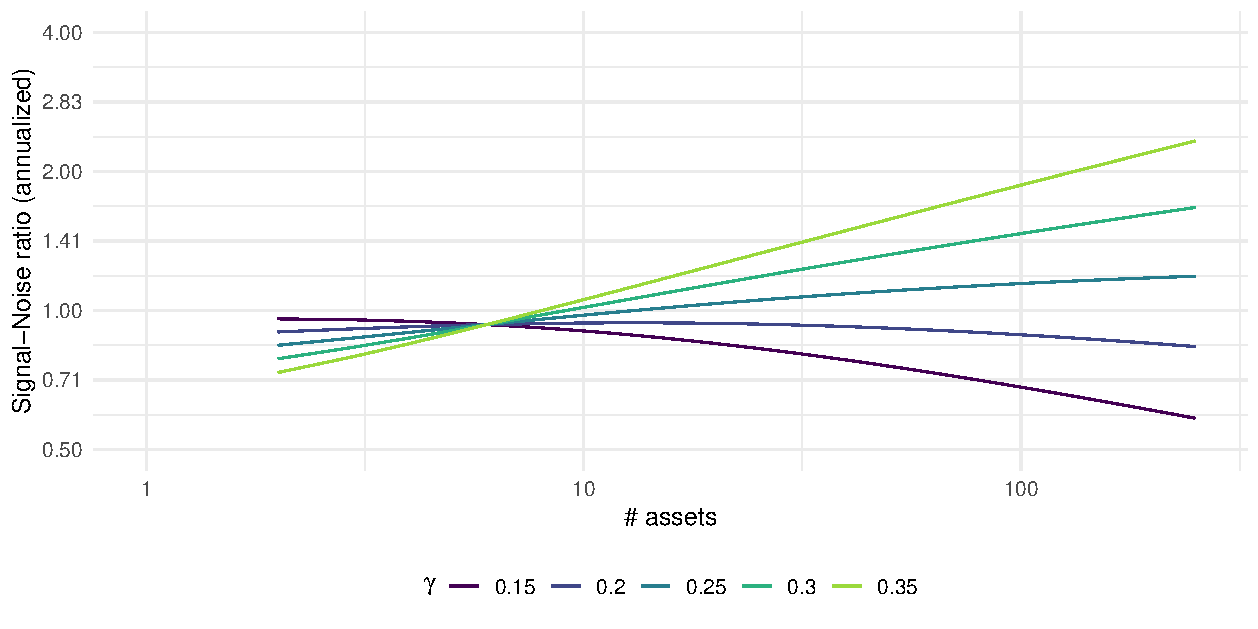
\includegraphics[width=0.99\textwidth,height=0.495\textwidth]{figure/qboundgrow_bound-1} \caption[The upper bound of \theoremref{qual_bound} is plotted versus \nlatf for different scaling laws.]{The upper bound of \theoremref{qual_bound} is plotted versus \nlatf for different scaling laws, corresponding to $\psnropt = \psnr[0]\nlatf^{\gamma}$, with $\gamma$ taking values between 0.15 and 0.35.}\label{fig:grow_bound}
\end{figure}

\end{knitrout}

The decreasing upper bound with respect to growing universe size
is illustrated in \figref{grow_bound}. Under the assumption
$\psnropt = \psnr[0]\nlatf^{\gamma}$, the upper bound
of \theoremref{qual_bound} is plotted versus \nlatf for 
different values of $\gamma$. 
The value of
$\psnr[0]$ is set so that 
$\psnropt=1.25\yrtomhalf$ when 
$\nlatf=6$.
For $\gamma < \oneby{4}$, one sees a local maximum in 
the upper bound as \nlatf increases, a behavior not seen for
$\gamma > \oneby{4}$, where the bound on \txtQual
grows with \nlatf. 


%$\psnropt$ and the $0.25, 0.50,$ and $0.75$ quantiles of
%$\psnropt\pql{\sportwfnc{\mreti}}$, under 
%\apxref{qual_dist}, are plotted versus \nlatf.
%The panels represent $\gamma$ values of
%$sort(pgammas)[1:(length(pgammas)-1)],$ and 
%$sort(pgammas)[length(pgammas)]$.
%The value of
%$\psnr[0]$ is set so that 
%$\psnropt=sqrt(ope)*zeta.s\yrtomhalf$ when 
%$\nlatf=n.stok$.
%For $\gamma < 0.25$, one sees a local maximum in 
%achieved \txtSR as \nlatf increases, a behavior not seen for
%$\gamma > 0.25$, where achieved \txtSR grows with \nlatf. 
%For the case of `slow growth' of \psnropt, the diversification 
%benefit is not seen by the sample \txtMP, rather its practical
%utility \emph{decreases} because the haircut outpaces the growth
%of \psnropt. As a practical matter, this may explain why the
%\txtMP is typically applied to small asset universes.



%% this is the approximate distribution of MP SR, which is now cutFOLDUP
%This relationship between \txtQual and \nlatf for different
%values of $\gamma$ appears not just in the upper bound of
%\theoremref{qual_bound}, but apparently also for most quantiles
%of the distribution given by \apxref{qual_dist}, as
%%This loss in value with respect to growing universe size is
%illustrated in \figref{grow_sqrt}. Again assuming
%$\psnropt = \psnr[0]\nlatf^{\gamma}$, lines of 
%$\psnropt$ and the $0.25, 0.50,$ and $0.75$ quantiles of
%$\psnropt\pql{\sportwfnc{\mreti}}$, under 
%\apxref{qual_dist}, are plotted versus \nlatf.
%The panels represent $\gamma$ values of
%$sort(pgammas)[1:(length(pgammas)-1)],$ and 
%$sort(pgammas)[length(pgammas)]$.
%Again, the value of
%$\psnr[0]$ is set so that 
%$\psnropt=sqrt(ope)*zeta.s\yrtomhalf$ when 
%$\nlatf=n.stok$.
%For $\gamma < \oneby{4}$, one sees a local maximum in 
%\txtQual as \nlatf increases, a behavior not seen for
%$\gamma > \oneby{4}$, where quantiles of \txtQual grow with \nlatf. 
%For the case of `slow growth' of \psnropt, the diversification 
%benefit is not seen by the sample \txtMP, rather its practical
%utility \emph{decreases} because the estimation error 
%outpaces the growth of \psnropt. 
%%UNFOLD

%Via the equivalence in \eqnref{sufficient_growth}, for the 
%bound \qbnd to be growing with respect to \nlatf, it suffices
%to establish that 
%$\half \le \wrapParens{\nlatf-1}\dbyd{\log\psnrsqopt}{\nlatf}$.
%From \eqnref{capm_zetas}, we have
%\begin{equation*}
%\begin{split}
%\half\dbyd{\log\psnrsqopt}{\nlatf} 
%&= 
%\frac{\trAB{\vect{\alpha}}{\dbyd{\vect{\alpha}}{\nlatf}} + 
%\wrapParens{\frac{\sigma_m}{\sigma}}^2 \wrapBracks{
 %\trAB{\vect{\beta}}{\dbyd{\vect{\beta}}{\nlatf}}\gram{\vect{\alpha}}
%+ \trAB{\vect{\alpha}}{\dbyd{\vect{\alpha}}{\nlatf}}\gram{\vect{\beta}}
%- \trAB{\vect{\alpha}}{\vect{\beta}}\wrapParens{
  %\trAB{\vect{\alpha}}{\dbyd{\vect{\beta}}{\nlatf}} + 
  %\trAB{\vect{\beta}}{\dbyd{\vect{\alpha}}{\nlatf}}}}}{%
%\gram{\vect{\alpha}} +
%\wrapParens{\frac{\sigma_m}{\sigma}}^2 \wrapBracks{%
%\gram{\vect{\beta}}\gram{\vect{\alpha}} -
%\wrapParens{\trAB{\vect{\alpha}}{\vect{\beta}}}^2}}
%+ \frac{\sigma_m^2 \trAB{\vect{\beta}}{\dbyd{\vect{\beta}}{\nlatf}}}{%
%\sigma^2 + \sigma_m^2\gram{\vect{\beta}}}.
%\end{split}
%\end{equation*}
%2FIX: where you going with this?
%These plots are built using \apxref{hcut_apx} ...

\subsection{Diversification under CAPM}%FOLDUP

It is not clear how \psnropt `should' scale with \nlatf. It is
easy to construct a model under which \psnropt scales as
$\nlatf^{\half}$: assume all assets have independent returns with
the same \txtSNR. It is also easy to accidentally construct 
a model under which \psnropt ultimately scales 
as $\nlatf^{\epsilon}$ for small $\epsilon$, as done here.
Suppose the \kth{i} asset has expected return
$\alpha_i$, exposure $\beta_i$ to `the market', and volatility
$\sigma$. Assume the market return is zero mean with volatility
$\sigma_m$. Then the squared \txtSNR is
\begin{align}
\nonumber
\psnrsqopt 
&= 
\frac{\gram{\vect{\alpha}} +
\wrapParens{\frac{\sigma_m}{\sigma}}^2 \wrapBracks{%
\gram{\vect{\beta}}\gram{\vect{\alpha}} -
\wrapParens{\trAB{\vect{\alpha}}{\vect{\beta}}}^2}}{\sigma^2 +
\sigma_m^2\gram{\vect{\beta}}},&\\
&= 
\frac{\gram{\vect{\alpha}}}{\sigma^2}
\frac{\sigma^2 + \sigma_m^2 \gram{\vect{\beta}} \fsin[2]{\psi}}{%
\sigma^2 + \sigma_m^2\gram{\vect{\beta}}},&
\label{eqn:capm_zetas}
\end{align}
where $\psi$ is the angle between the vectors \vect{\alpha}
and \vect{\beta}.
Depending on how the sine of $\psi$ grows with universe size, 
one observes different scaling of \psnropt with respect to \nlatf. When
the assets all have the same alpha and beta, \ie
$\vect{\alpha} = \alpha\vone$ and $\vect{\beta} = \beta\vone$,
the sine is identically zero, and 
$\psnropt = \sqrt{\fraccp{\nlatf\alpha^2}{\sigma^2 + \nlatf\sigma_m^2\beta^2}}
< \alpha\beta^{-1}\sigma_m^{-1}$. Thus 
\psnropt asymptotically scales slower than $\nlatf^{\epsilon}$
for all $\epsilon > 0$.

On the other hand, when the sine is
one, \ie when \vect{\alpha} is orthogonal to \vect{\beta},
$\psnropt = \sqrt{\gram{\vect{\alpha}}} \sigma^{-1}$, which
grows however the assets are ordered, presumably on the
order of $\nlatf^{\half}$. Thus under a CAPM model, the
growth of \psnropt depends on the `alignment' of the
vectors \vect{\alpha} and \vect{\beta}.
%UNFOLD

%UNFOLD

%%%%%%%%%%%%%%%%%%%%%%%%%%%%%%%%%%%%%%%%%%%%%%%%%%%%%%%%%%%%%%%%%%%%%%%%
\section{Generalizations}%FOLDUP

\label{sec:generalizations}

\theoremref{qual_bound} is somewhat lacking because it ignores conditioning
information which may affect the distribution of future returns, and which
may inform the portfolio manager. Few active managers, it is presumed,
are holding the unconditional \txtMP based on in-sample data. What is sought
is a more general theorem that allows more elaborate models of returns,
and more elaborate, parametrized, trading schemes, with \psnropt redefined 
as the maximal portfolio \txtQual over the trading schemes, and \nlatf
redefined as the `degrees of freedom', perhaps the rank of some derivative
at the optimal parameter, say. Towards that goal, a few generalizations can
easily be made.

\subsection{Conditional portfolio \txtQual}%FOLDUP
\label{subsec:cond_portfolio_qual}

The model of stationary mean returns is generalized by one where
the expected return of the assets is linear in some state
variables, or `features', \vfact[i], observed prior to the investment
decision.  \cite{pav_the_book,connor1997,herold2004TAA} That
is, one observes the \nfac-vector $\vfact[i]$ at some time prior to 
when the investment decision is required to capture \vreti[i+1]. 
The general model is now
\begin{align}
\label{eqn:cond_model_IV}
\Econd{\vreti[i+1]}{\vfact[i]} &=
\pRegco \vfact[i], &
\Varcond{\vreti[i+1]}{\vfact[i]} &=
\pvsig,
\end{align}
where \pRegco is some \bby{\nlatf}{\nfac} matrix. 

Here we bound the \txtQual of portfolios which are
linear in the features \vfact[i]. That is, the portfolio
manager allocates their assets proportional to
$\sportW\vfact[i]$ for some matrix $\sportW$.

Using the law of iterated expectations, the unconditional
expected value of the returns of the portfolio is
\begin{equation*}
\E{\Econd{\trAB{\wrapParens{\sportW\vfact[i]}}{\vreti[i+1]}}{\vfact[i]}}
= \trace{\tr{\sportW}\pRegco\E{\ogram{\vfact[i]}}}
= \trace{\tr{\sportW}\pRegco\pfacsig},
\end{equation*}
by definition of \pfacsig as the second moment of \vfact[i].

Unfortunately the unconditional variance will, in general,
involve a term quadratic in the expectation. However, it
can easily be shown that the unconditional \emph{expected} 
variance of the portfolio's returns is
\begin{equation*}
\E{\qform{\pvsig}{\wrapParens{\sportW\vfact[i]}}} =
\trace{\qform{\pvsig}{\sportW}\pfacsig}.
\end{equation*}
We can then redefine\footnote{If an analysis of the conditional expected
return divided by risk is required, it is possible one could define
\pQl{\cdot} as the expected return divided by square root of the unconditional
second moment. The \txtQual would then be $\ftan{\farcsin{\pQl{\cdot}}}$.
One could possibly find a \txtCR bound on the expected value of this \pQl{\cdot}.
This `Pillai-Bartlett' form of \pQl{\cdot} is likely unrequired for low frequency
settings.} the \txtQual of the portfolio as the
unconditional mean divided by the unconditional expected risk:
\begin{equation}
\pQl{\sportW}\defeq\frac{\trace{\tr{\sportW}\pRegco\pfacsig}}{%
\sqrt{\trace{\qform{\pvsig}{\sportW}\pfacsig}}}.
\end{equation}
When \vfact[i] is a deterministic scalar constant, 
this coincides with the `usual' definition of \txtQual as being 
like a \txtSR. However, except possibly for an intercept term, one
expects \vfact[i] to be random, or at least out of the control of
the portfolio manager.

Once again, a risk transform can be injected to express
portfolio optimization as an estimation problem on a sphere:
\begin{equation}
\begin{split}
\pQl{\sportW}
&=\frac{\trace{\trAB{%
\wrapParens{\trchol{\pvsig}\sportW\chol{\pfacsig}}}{%
\wrapParens{\ichol{\pvsig}\pRegco\chol{\pfacsig}}}{%
}}}{%
\sqrt{\trace{
\gram{\wrapParens{\trchol{\pvsig}\sportW\chol{\pfacsig}}}}}},\\
&=
\frac{\trAB{\fvec{\trchol{\pvsig}\sportW\chol{\pfacsig}}}{%
\fvec{\ichol{\pvsig}\pRegco\chol{\pfacsig}}}}{%
\sqrt{\gram{\fvec{\trchol{\pvsig}\sportW\chol{\pfacsig}}}}}.
\end{split}
\end{equation}
This function is maximized by taking
\begin{equation}
\sportW = \pportWopt \defeq \minv{\pvsig}{\pRegco},
\end{equation}
which has \txtQual
\begin{equation}
\psnropt\defeq\pQl{\pportWopt} =
\sqrt{\trace{\qiform{\pvsig}{\pRegco}\pfacsig}}.
\end{equation}
The square of this quantity, \psnrsqopt, 
is the `population analogue' of the Hotelling-Lawley trace. \cite{Rencher2002,Muller1984143}

Again we can write
\begin{equation*}
\frac{\pQl{\sportW}}{\psnropt} = 
\trAB{\fnorm{\fvec{\trchol{\pvsig}\sportW\chol{\pfacsig}}}}{%
\fnorm{\fvec{\ichol{\pvsig}\pRegco\chol{\pfacsig}}}}.
\end{equation*}
Thus finding a `good' \sportW becomes an estimation problem on the
sphere \sphere{\nfac\nlatf - 1}. An analogue
to \theoremref{qual_bound} can be proved with $\nfac\nlatf$ replacing
$\nlatf$, by assuming a particular form to the likelihood. We must
generalize the assumption of Directional Independence, after which
the theorem proceeds easily.

\begin{assumption}[Conditional Directional Independence]%FOLDUP
Assume that
\begin{equation}
\label{eqn:sane_estimator_cond}
\E{\fnorm{\fvec{\trchol{\pvsig}\sportWfnc{\mreti,\mfact}}}} = 
\cfnc{\psnrsqopt} \fnorm{\fvec{\trchol{\pvsig}\pportWopt\chol{\pfacsig}}}
+ \Bterm,
\end{equation}
where \Bterm is the bias term, orthogonal to 
\fnorm{\fvec{\trchol{\pvsig}\pportWopt\chol{\pfacsig}}}.
\end{assumption}%UNFOLD

\begin{theorem}%FOLDUP
\label{theorem:qual_bound_two}
Let one element of \vfact[i] be a deterministic $1$. Suppose the
vector of the remaining $\nfac-1$ elements of \vfact[i] stacked 
on top of \vreti[i+1] are multivariate Gaussian.  Let \mreti, 
\mfact be \bby{\ssiz}{\nlatf} and \bby{\ssiz}{\nfac} matrices
of \iid observations of the features and returns.
Let \sportWfnc{\mreti,\mfact} be an estimator 
%based on 
%\ssiz \iid observations of multivariate Gaussian returns, \mreti, 
%and multivariate Gaussian features, \mfact, with one column of \mfact
%an intercept term, 
satisfying the assumptions of
Conditional Directional Independence and Residual Independence. Then
\begin{equation}
\E{\pQl{\sportWfnc{\mreti,\mfact}}} 
\le \frac{\sqrt{\ssiz}\psnrsqopt}{\sqrt{\nfac\nlatf - 1 + \ssiz\psnrsqopt}}.
\end{equation}
\end{theorem}%UNFOLD
\begin{proof}%FOLDUP

We can proceed as in \secref{portfolio_qual}. Let \mreti be the 
\bby{\ssiz}{\nlatf} matrix of portfolio returns, and let 
\mfact be the corresponding \bby{\ssiz}{\nfac} matrix of features.
View the portfolio coefficient \sportW as an estimator, a function of
the random data, \ie \sportWfnc{\mreti,\mfact}.
%Assume
%Directional Independence, with \eqnref{sane_estimator}
%becoming
%\begin{equation}
%\E{\fnorm{\trchol{\pvsig}\sportWfnc{\mreti,\mfact}}} = 
%\cfnc{\psnrsqopt} \fnorm{\trchol{\pvsig}\pportWopt\chol{\pfacsig}}
%+ \Bterm.
%\end{equation}
Define
\begin{equation}
\prskMtx\defeq{\ichol{\pvsig}\pRegco\chol{\pfacsig}}.
\end{equation}
Then 
\begin{equation*}
\psnrsqopt = \trace{\gramprskMtx}.
\end{equation*}

We get, analogously to \eqnref{crb_one},
\begin{equation}
\oneby{\ssiz}\trace{\qoform{\iFishI[\fvec{\prskMtx}]}{\Drv}}
\le 1 - \csqfnc{\trace{\gramprskMtx}},
\end{equation}
where
\begin{equation}
\Drv\defeq
{\dbyd{\cfnc{\trace{\gramprskMtx}}\frac{\prskMtx}{\sqrt{\trace{\gramprskMtx}}}}{\fvec{\prskMtx}}}.
\end{equation}

Without loss of generality, we assume it is the first element
of \vfact[i] that is a deterministic $1$. Then, the log likelihood of 
the vector of $\vfact[i]$ stacked on top of $\vreti[i+1]$
is: \cite{pav2013markowitz}
\begin{equation}
\label{eqn:cond_llik_one}
\log \FOOlik{}{\pvsm}{\twobyone{\vfact[i]}{\vreti[i+1]}} = 
  c_{\nfac+\nlatf} 
- \half \logdet{\pvsm} 
- \half \trace{\minv{\pvsm}\ogram{\twobyone{\vfact[i]}{\vreti[i+1]}}},
\end{equation}
where \pvsm is the second moment matrix:
\begin{equation}
\pvsm \defeq \E{\ogram{\twobyone{\vfact[i]}{\vreti[i+1]}}}
= \twobytwo{\pfacsig}{\pfacsig\tr{\pRegco}}{\pRegco\pfacsig}{\pvsig +
\qoform{\pfacsig}{\pRegco}}.
%\qoform{\pfaccov}{\pRegco}}}.
\end{equation}
The inverse of \pvsm has the following, somewhat surprising, form \cite{pav2013markowitz}:
\begin{equation}
\minv{\pvsm} 
= \twobytwo{\minv{\pfacsig} +
\qiform{\pvsig}{\pRegco}}{-\tr{\pRegco}\minv{\pvsig}}{-\minv{\pvsig}\pRegco}{\minv{\pvsig}}.
\end{equation}
A square root of this matrix (a Cholesky factor, up to permutation)
is:
\begin{equation}
\begin{split}
\minv{\pvsm} &=
\ogram{%
\twobytwo{\ichol{\pfacsig}}{-\tr{\pRegco}\ichol{\pvsig}}{\mzero}{\ichol{\pvsig}}
},\\
&= \twobytwo{\ichol{\pfacsig}}{\mzero}{\mzero}{\eye}
\ogram{%
\twobytwo{\eye}{-\prskMtxU{\trsym}}{\mzero}{\ichol{\pvsig}}}
\twobytwo{\trichol{\pfacsig}}{\mzero}{\mzero}{\eye}.
\end{split}
\end{equation}

By the block determinant formula, 
\begin{equation}
\det{\pvsm} 
= \det{\pfacsig}\det{\pvsig + \qoform{\pfacsig}{\pRegco} -
\pRegco\pfacsig\minv{\pfacsig}\pfacsig\tr{\pRegco}}
= \det{\pfacsig}\det{\pvsig}.
\end{equation}
Thus, conditional on \pfacsig and \pvsig, the negative log likelihood
takes the form:
\begin{multline}
\label{eqn:cond_llik_two}
- \log \FOOlik{}{\prskMtx, \pfacsig, \pvsig}{\twobyone{\vfact[i]}{\vreti[i+1]}} = 
- c_{\nfac+\nlatf}
+ \half \logdet{\pfacsig} 
+ \half \logdet{\pvsig}\\
+ \half \trace{
\ogram{%
\twobytwo{\eye}{-\prskMtxU{\trsym}}{\mzero}{\ichol{\pvsig}}}
\ogram{\twobyone{\trichol{\pfacsig}\vfact[i]}{\vreti[i+1]}}}.
\end{multline}
Sweeping the nuisance parameter terms into the constant, as well
as terms in the trace which are not quadratic in \prskMtx, we
have 
\begin{align}
\label{eqn:cond_llik_three}
- \log \FOOlik{}{\prskMtx, \pfacsig, \pvsig}{\twobyone{\vfact[i]}{\vreti[i+1]}}
&= - c'
+ \half \trace{\gramprskMtx 
\ogram{\wrapParens{\trichol{\pfacsig}\vfact[i]}}},&\\
&= - c'
+ \half
\tr{\fvec{\prskMtx}}\fvec{\prskMtx\trichol{\pfacsig}\ogram{\vfact[i]}\ichol{\pfacsig}}.&\\
&= - c'
+ \half
\tr{\fvec{\prskMtx}}\wrapParens{%
\wrapBracks{\trichol{\pfacsig}\ogram{\vfact[i]}\ichol{\pfacsig}}
 \kron \eye}\fvec{\prskMtx}.&
\end{align}
The Fisher Information, then, is
\begin{equation}
\FishI[\fvec{\prskMtx}] =
\E{\wrapParens{%
\wrapBracks{\trichol{\pfacsig}\ogram{\vfact[i]}\ichol{\pfacsig}}
 \kron \eye}} = \eye[\nfac\nlatf].
\end{equation}

The remainder of the proof proceeds exactly as in 
\secref{portfolio_qual}. 
\end{proof}%UNFOLD

%\begin{theorem}
%\label{theorem:qual_bound_two}
%Let \sportWfnc{\mreti,\mfact} be an estimator based on 
%\ssiz \iid observations of multivariate Gaussian returns, \mreti, 
%and multivariate Gaussian features, \mfact, with one column of \mfact
%an intercept term, satisfying the assumptions of
%directional independence and residual independence. Then
%\begin{equation}
%\E{\pQl{\sportWfnc{\mreti,\mfact}}} 
%\le \frac{\sqrt{\ssiz}\psnrsqopt}{\sqrt{\nlatf\nfac - 1 + \ssiz\psnrsqopt}}.
%\end{equation}
%\end{theorem}

%&= \E{\Cmat\scoro{\prskvec}{\FOOlik{}{\prskvec}{\mreti}}

%\begin{equation}
%\begin{split}
%\vfact[i] &\sim \normlaw{\pfacmu, \pfaccov},\\
%\condtwo{\vreti[i+1]}{\vfact[i]} &\sim \normlaw{\pRegco\vfact[i], \pvsig}.
%\end{split}
%\end{equation}
%Together the unconditional distribution is
%\begin{equation}
%\twobyone{\vfact[i]}{\vreti[i+1]} \sim
%\normlaw{\twobyone{\pfacmu}{\pRegco\pfacmu}, 
%\twobytwo{\pfaccov}{\pfaccov\tr{\pRegco}}{\pRegco\pfaccov}{\pvsig +
%\qoform{\pfaccov}{\pRegco}}}.
%\end{equation}




%In this model, the `Markowitz Coefficient' 
%$\minvAB{\pvsig}{\pRegco}$, generalizes the \txtMP as
%the coefficient of the optimal portfolio which is linear in \vfact,
%under some objective. \cite{pav2013markowitz} How should we define
%the \txtQual of the Markowitz Coefficient, and can we prove
%an analogue of \theoremref{qual_bound}?
%UNFOLD

\subsection{Subspace constraints}%FOLDUP

Consider, now, the case of conditional expectation, as presented in
\subsecref{cond_portfolio_qual}, but where the portfolio is 
constrained to be in some lower dimensional subspace. That is, by design, 
\begin{equation}
\zerJc \sportWfnc{\mreti,\mfact} = \vzero,
\end{equation}
where $\zerJc$ is a \bby{\wrapParens{\nlatf - \nlatfzer}}{\nlatf}
matrix of rank $\nlatf - \nlatfzer$, that is chosen independently
of the observations of \mreti and \mfact.
Let the rows of \zerJ span the null space of the rows of
\zerJc; that is, $\zerJc \tr{\zerJ} = \mzero$, and $\ogram{\zerJ} = \eye$.

We can simply use the results of \subsecref{cond_portfolio_qual}, but
replacing the assets with the \nlatfzer assets spanned by the rows of
\zerJ. That is, we can replace the \vreti[i+1] with $\zerJ\vreti[i+1]$,
and replace \sportWfnc{\mreti,\mfact} with
$\tr{\zerJ}\minv{\wrapParens{\ogram{\zerJ}}}\sportWfnc{\mreti,\mfact}$
to arrive at the following analogue of \theoremref{qual_bound_two}:

\begin{theorem}%FOLDUP
\label{theorem:qual_bound_three}
Let one element of \vfact[i] be a deterministic $1$. Suppose the
vector of the remaining $\nfac-1$ elements of \vfact[i] stacked 
on top of \vreti[i+1] are multivariate Gaussian.  Let \mreti, 
\mfact be \bby{\ssiz}{\nlatf} and \bby{\ssiz}{\nfac} matrices
of \iid observations of the features and returns.
Let \sportWfnc{\mreti,\mfact} be an estimator 
%based on 
%\ssiz \iid observations of multivariate Gaussian returns, \mreti, 
%and multivariate Gaussian features, \mfact, with one column of \mfact
%an intercept term, 
satisfying the assumptions of
directional independence and residual independence, with the constraint
\begin{equation}
\zerJc \sportWfnc{\mreti,\mfact} = \vzero,
\end{equation}
for \bby{\wrapParens{\nlatf - \nlatfzer}}{\nlatf} matrix \zerJc, which
is chosen independently of the observed \mreti and \mfact. 
Let the rows of \zerJ span the null space of the rows of
\zerJc. 

Then
\begin{equation}
\E{\pQl{\sportWfnc{\mreti,\mfact}}} 
\le \frac{\sqrt{\ssiz}\psnrsqoptG{\zerJ}}{\sqrt{\nfac\nlatfzer - 1 +
\ssiz\psnrsqoptG{\zerJ}}},
\end{equation}
where 
\begin{equation*}
\psnrsqoptG{\zerJ}\defeq 
\trace{\qform{\wrapProj{\pvsig}{\zerJ}}{\pRegco}\pfacsig}.
\end{equation*}
\end{theorem}%UNFOLD
%UNFOLD

\subsection{Hedging constraints}%FOLDUP

Consider, now, the case where one seeks a portfolio whose returns are
independent, in the probabilistic sense, of the returns of some 
traded instruments in the investment universe. 
Independence is a difficult property to
check or enforce; however, independence implies zero covariation, which
can be easily formulated and checked. 

Since the portfolio estimator may not deliver a perfectly
hedged portolio due to misestimation of the covariance matrix, we
will, with perfect knowledge of \pvsig, consider the \txtQual of the 
hedged part of the portfolio. The hedged
part is defined in terms of a risk projection. 
If \sportw[1] is a feasible portfolio based on the sample,
then the hedged version of this portfolio is the solution to the
optimization problem
\begin{equation}
\min_{\sportw : \hejG\pvsig\sportw = \vzero} \VAR{\trAB{\wrapParens{\sportw -
\sportw[1]}}{\vreti[i+1]}},
\end{equation}
where $\hejG$ is a \bby{\nlatfhej}{\nlatf} matrix of 
rank \nlatfhej, the rows of which we wish to `hedge out.'

Using the Lagrange multiplier technique, this can easily be found to
be solved by 
\begin{equation}
\sportw = \sportw[1] - \wrapProj{\pvsig}{\hejG}\pvsig\sportw[1].
\end{equation}
Thus we will consider the \txtQual of the portfolio estimator
\begin{equation*}
\wrapParens{\eye[\nlatf] - \wrapProj{\pvsig}{\hejG}\pvsig}\sportWfnc{\mreti,\mfact}.
\end{equation*}
Note, however, that the row rank of
$\wrapParens{\eye[\nlatf] - \wrapProj{\pvsig}{\hejG}\pvsig}$ 
is $\nlatf - \nlatfhej$.  Thus hedging is an instance of a subspace
constraint and we can apply \theoremref{qual_bound_three} outright.

\begin{theorem}%FOLDUP
\label{theorem:qual_bound_four}
Let one element of \vfact[i] be a deterministic $1$. Suppose the
vector of the remaining $\nfac-1$ elements of \vfact[i] stacked 
on top of \vreti[i+1] are multivariate Gaussian.  Let \mreti, 
\mfact be \bby{\ssiz}{\nlatf} and \bby{\ssiz}{\nfac} matrices
of \iid observations of the features and returns.
Let \sportWfnc{\mreti,\mfact} be an estimator 
%based on 
%\ssiz \iid observations of multivariate Gaussian returns, \mreti, 
%and multivariate Gaussian features, \mfact, with one column of \mfact
%an intercept term, 
satisfying the assumptions of
directional independence and residual independence. 
Let \bby{\nlatfhej}{\nlatf} matrix \hejG be chosen
independently of \mreti and \mfact. 

%2FIX: redefine Deltapsnr to not be confusing.
Define 
\begin{equation}
\Delpsnrsqopt{\eye,\hejG}
\defeq
\trace{\qiform{\svsig}{\pRegco}\pfacsig} - 
\trace{\qform{\wrapProj{\pvsig}{\hejG}}{\pRegco}\pfacsig}.
\end{equation}

Then
\begin{equation}
\E{\pQl{%
\wrapBracks{\eye[\nlatf] - \wrapProj{\pvsig}{\hejG}\pvsig}\sportWfnc{\mreti,\mfact}}} 
\le \frac{\sqrt{\ssiz}\Delpsnrsqopt{\eye,\hejG}}{\sqrt{\nfac\wrapParens{\nlatf -
\nlatfhej} - 1 + \ssiz\Delpsnrsqopt{\eye,\hejG}}}.
\end{equation}
\end{theorem}%UNFOLD

%UNFOLD

%UNFOLD

%%%%%%%%%%%%%%%%%%%%%%%%%%%%%%%%%%%%%%%%%%%%%%%%%%%%%%%%%%%%%%%%%%%%%%%%
\section{Examples}%FOLDUP

\subsection{The equal weight puzzle}%FOLDUP


\theoremref{qual_bound} can help us make sense of puzzling findings
in the literature. For example, in the ``$1/N$'' paper, DeMiguel \etal
find that the equal-weighting portfolio outperforms, in terms of out-of-sample
\txtSR (and other measures), the \txtMP and numerous other portfolio
estimators.  \cite{demiguel2009optimal}
This finding is supported on a number of real world data
sets, and a few synthetic ones. One data set used was the returns of
the 10 industry portfolios and the US equity market portfolio, computed
by Ken French. 
% 2FIX: add citation to data.

The monthly returns, from 1927-01-01 to 
2020-12-01, for these 10 
assets were downloaded
from Kenneth French's data library.  \cite{French10Port}
%from \emph{Quandl}.  \cite{Quandl}
The \txtSR of the equal weighted portfolio on the %10
assets, over the 1128 months, is around 
$0.67\yrtomhalf$. The \txtSR of the sample \txtMP over
the 10 assets over the same period is around
$0.86\yrtomhalf$.  
Now consider a portfolio estimator
given 5 years of observations, as in 
DeMiguel \etal \cite{demiguel2009optimal}, assuming 
$\psnropt=0.86\yrtomhalf$.
The bound on expected value of \pql{\sportwfnc{\mreti}} from \theoremref{qual_bound} is only $0.46\yrtomhalf$.  
%Under \apxref{qual_dist}, the probability that \pql{\sportwfnc{\mreti}} exceeds $sr1$sr\yrtomhalf$ in this case is only $dfp$. 
It is not surprising that DeMiguel \etal drew
the conclusions they did, nor that they would be refuted
by looking at a longer sample, as by Kritzman \etal \cite{defoopt2010}



One could also use \theoremref{qual_bound_four} here. However,
the upper bound of that theorem is non-negative, and zero only
if the quantity \Delpsnrsqopt{\eye,\hejG} is zero.  This is a
statement regarding unknown population parameters, but we can
perform inference on this quantity. For example, based on the
1128 months of data on these 
10, the 95\% confidence interval on
\Delpsnrsqopt{\eye,\hejG}, where \hejG is the \bby{1}{10}
matrix of all ones, is
$\asrowvec{0.04, 0.45}\yrto{-1}$, under the assumption of
Gaussian returns.  

%One could view the touted superiority of the equal weight portfolio
%over \eg the \txtMP as a veiled claim that there is a single
%discount factor that rules all asset returns. As stated, this claim
%is clearly absurd, since \eg an equal weight portfolio on both pairs
%of leveraged ETFs is clearly inferior to a portfolio equal weight \emph{short}
%both pairs.  \cite{zhang2010path}

%This highlights
%the fact that the putative superiority of the equal weight portfolio
%may be based on two due less to deficiencies in \eg the \txtMP, and more to
%the 

%The analysis presented here is likely to be optimistic when one
%considers the \emph{spanning} aspect of this problem.  
%\cite{giri1964likelihood,HKspan1987,KanZhou2012} That is, the
%total effect size beyond the equal weighting subspace may be
%very small. A `proper' analysis would take into account the
%difference in effect sizes and differences in universe size. 
%However, the spanning analogue of \theoremref{qual_bound}
%has not yet been established.

%% 2FIX: talk about the spanning statistics here. is there
%% any effect to exploit?
%The result is dKRS or
%dUNB or
%dMLE.
%the upper bound is asqb.
%Show it as:
%dsr2
%or cis: myci.

%UNFOLD

\subsection{Empirical diversification in the S\&P 100}%FOLDUP



To check how \psnropt \emph{might} scale with \nlatf, the weekly
log returns of the adjusted close prices of the stocks in the 
S\&P 100 Index, as of March 21, 2014, were downloaded 
from \emph{Quandl}.  \cite{Quandl} 
Adjustments for splits and
dividends were made in some unspecified way by the upstream source
of the data, Yahoo Finance. Stocks without a full 5 years of history
were discarded, leaving 96 stocks. 
Note that selection based on membership in the index at the end of the 
period adds no small amount of selection bias, which we shall ignore 
here.

Based on the weekly returns from 2009-03-27 to 2014-04-04,
estimates of \psnropt were computed, using the `KRS' estimator.
\cite{kubokawa1993estimation,pav_the_book} 
This was performed on the first \nlatf assets, with \nlatf ranging from 
$1$ to $96$.  The estimate of \psnropt versus \nlatf
is plotted in \figref{sp100_grow}, with assets added in alphabetical order.
Because Apple appears at the beginning of this list, it appears that
\psnropt starts reasonably large, but then actually \emph{decreases}
when adding assets. This is an artifact of the estimator, since the true
\psnropt can only increase when adding assets. 

\begin{knitrout}\small
\definecolor{shadecolor}{rgb}{0.969, 0.969, 0.969}\color{fgcolor}\begin{figure}[h]
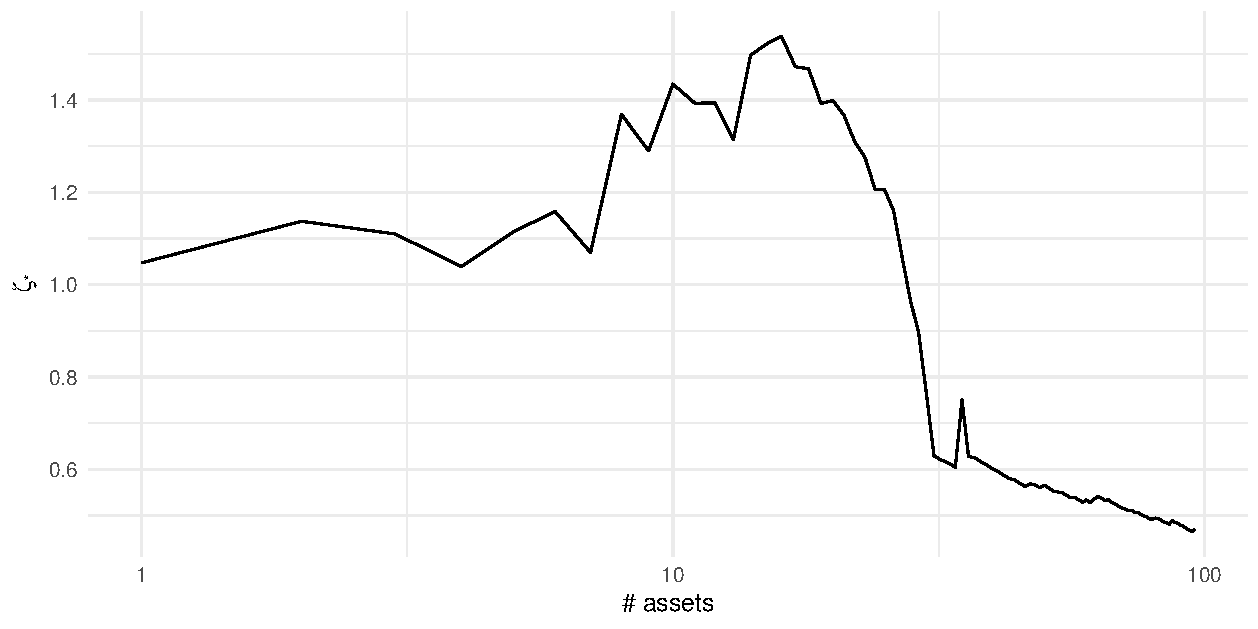
\includegraphics[width=0.99\textwidth,height=0.495\textwidth]{figure/qboundsp100_grow-1} \caption[Growth of estimated \psnropt versus \nlatf for the S\&P 100 Index names, in alphabetical order, showing the `Apple effect.']{Growth of estimated \psnropt versus \nlatf for the S\&P 100 Index names, in alphabetical order, showing the `Apple effect.'}\label{fig:sp100_grow}
\end{figure}

\end{knitrout}

%<<'sp100_mid',eval=TRUE,cache=FALSE,fig.width=5.75,fig.height=3.75,dpi=450,fig.cap=paste0("Growth of estimated \\psnropt versus \\nlatf for the S\\&P 100 Index names."),eval.after='fig.cap'>>= 

%foo.df <- data.frame(df=(1:length(KRSs)),KRS=KRSs,
		%MLE=MLEs,meanKRS=rowMeans(buncho.KRSs))

%require(ggplot2)
%ph <- ggplot(data=foo.df,aes(x=df,y=meanKRS))
%ph <- ph + geom_line()
%ph <- ph + labs(x="# assets",
								%y=expression(zeta["*"]))
%ph <- ph + scale_x_log10()
%ph <- ph + scale_y_log10()
%print(ph)

%@

Since the ordering of assets here is arbitrary, the experiment was repeated
1000 times, with the stocks randomly permuted, and 
\psnropt estimated as a function of \nlatf. Boxplots, over the
1000 simulations, of the KRS statistic versus
\nlatf are given in \figref{sp100_box}. There is effectively no 
diversification benefit observed here beyond the mean effect, which is
equivalent to holding an equal weight portfolio. Given the 
conditions under which \txtQual grows with \nlatf outlined in 
\secref{diversification}, one expects poor performance of 
directionally independent portfolio estimators
over even a small subset of the S\&P 100.

\begin{knitrout}\small
\definecolor{shadecolor}{rgb}{0.969, 0.969, 0.969}\color{fgcolor}\begin{figure}[h]
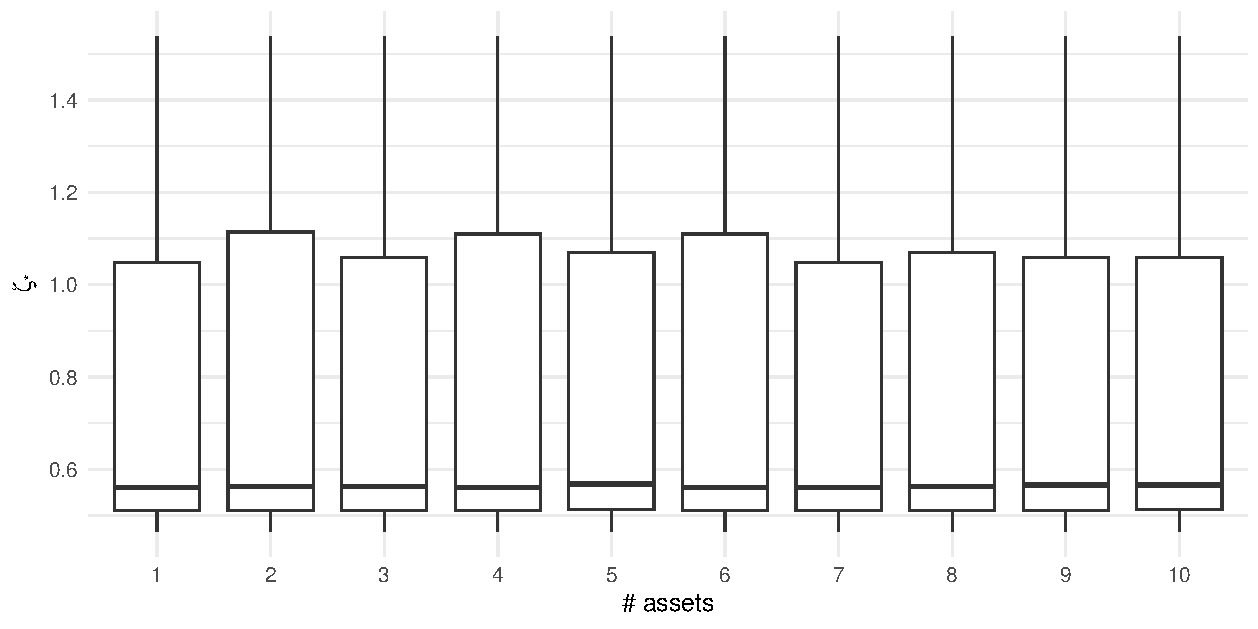
\includegraphics[width=0.99\textwidth,height=0.495\textwidth]{figure/qboundsp100_box-1} \caption[Growth of estimated \psnropt versus \nlatf for the S\&P 100 Index names is shown over 1000 permutations of the stocks, showing that there is effectively \emph{no} diversification benefit here beyond an equal weight portfolio]{Growth of estimated \psnropt versus \nlatf for the S\&P 100 Index names is shown over 1000 permutations of the stocks, showing that there is effectively \emph{no} diversification benefit here beyond an equal weight portfolio.}\label{fig:sp100_box}
\end{figure}

\end{knitrout}
%UNFOLD
%UNFOLD

%%%%%%%%%%%%%%%%%%%%%%%%%%%%%%%%%%%%%%%%%%%%%%%%%%%%%%%%%%%%%%%%%%%%%%%%
\section{Discussion}%FOLDUP

Care should be taken in the interpretation of \theoremref{qual_bound},
or its generalizations from \secref{generalizations}.
It does not claim that the sample \txtMP is somehow `optimal,' nor
does it make comparative claims about different portfolio estimators
when presented with the same data.
The theorem does not imply that somehow `overfitting' to the observed
data can be mitigated by selecting a less desireable portfolio. 
It does not claim that sample estimates of the \txtQual of a portfolio
are useless.  It is trivially
the case, for example, that if $\pql{\sportw[1]} > \pql{\sportw[2]}$, then,
with probability greater than half, 
$\trAB{\sportw[1]}{\svmu} / \sqrt{\qform{\svsig}{\sportw[1]}} > 
\trAB{\sportw[2]}{\svmu} / \sqrt{\qform{\svsig}{\sportw[2]}}$, where
the probability is over draws of \svmu and \svsig.
The theorem does not claim that the expected
\txtQual of a portfolio estimator is negative. (Indeed, it can not,
since the portfolio estimator which generates a random portfolio, 
ignoring the data, has zero expected \txtQual). 
The theorem makes no claims (\eg providing a Bayesian posterior) about 
any particular portfolio based on a single sample of the data: it is
a statement about the expectation of the \emph{estimator} under replication 
of draws of the sample.

One should recognize, moreover, there are situations where the assumptions
of the theorem are violated. For example, in some cases a prior 
bias for positive expected returns, \ie $\pvmu \ge 0$, is warranted,
and thus a portfolio estimator with a long bias is chosen.
This can happen when the underlying assets are equities, and
the eligible universe is based on some minimum longevity, as this 
introduces a `good' survivorship bias: 
companies with negative expected return should founder and perish, 
leaving behind those with more positive $\pmu$. Effectively this
acts to boost \ssiz somewhat, although the effect is likely small.

There are other reasonable portfolio estimators which violate the 
assumption of Directional Independence. For example, an estimator
which performs some dimensionality reduction based on the observed
data, \mreti and \mfact will not be covered by 
\theoremref{qual_bound_three} since the subspace is chosen based
on the sample. However, it might not be covered by 
\theoremref{qual_bound_two} because the expected \txtQual might
depend on how \pRegco aligns with the leading eigenvectors of
\pvsig, say.

\subsection{Future work}%FOLDUP

These findings perhaps raise more questions than they answer:
%This work leaves unanswered a number of interesting questions:
\begin{compactenum}
\item Foremost, the bounds of 
\theoremref{qual_bound} and \theoremref{qual_bound_two}
depend on the unknown
quantity, \psnrsqopt. How can we perform inference, 
Frequentist or Bayesian, on \pql{\sportwopt}, where \sportwopt is the \txtMP, 
given the observed information (\viz \svmu and \svsig)? This
is a problem of enormous practical concern to hundreds of
quantitative portfolio managers.

Contrast inference on the portfolio \txtQual with inference
on the population \txtSNR: under Gaussian returns, the
distribution of \ssrsqopt in terms of \ssiz, \nlatf and \psnrsqopt
is known. \cite[Theorem 5.2.2]{anderson2003introduction}
Thus, for example, the quantity
$\wrapParens{1 - \fracc{\nlatf}{\ssiz}}\ssrsqopt - \fracc{\nlatf}{\ssiz}$
is an unbiased estimator for \psnrsqopt, \etc 
Performing inverence on \pql{\sportwopt} is tricky because \psnrsqopt
is unknown and the error $\sportwopt - \pportwopt$ is likely
not independent of the error in the estimate \ssropt.

It may be the case, however, that inference on the portfolio
\txtQual qualifies as an `impossible' estimation-after-selection
problem. \cite{leeb2006}
\item While \theoremref{qual_bound} requires Gaussian returns, 
one expects that the result holds for returns distributions whose 
likelihood is ``more concave'' than the Gaussian at the MLE.
Exact conditions for this to hold should be established.
%\item How is \txtQual affected by the imposition of hedging and
%other constraints?  \cite{pav2013markowitz} Does dimensionality
%reduction modify the `degrees of freedom' in the straightforward
%way? Is there an analogue of the bound for portfolio
%spanning?  \cite{giri1964likelihood,HKspan1987,KanZhou2012}
%That is, can we find a bound on $\E{\pql{\sportw[2]} - \pql{\sportw[1]}}$,
%where \sportw[1] is a portfolio on a subspace of the assets over
%which \sportw[2] is selected, with the bound depending on the 
%spanning parameter, $\psnrsqoptG{2} - \psnrsqoptG{1}$?
\item \theoremref{qual_bound_two} applies to the case of 
trading strategies where the portfolio is linear in the 
observable features, \vfact[i]. 
Can it be used as an approximate bound for trading
strategies which are nonlinear, complex functions of the features?
\item 
What can be said about scaling of \psnropt with respect to
\nlatf for different models of market returns? 
Can one establish
reasonable sufficient conditions for which \psnropt grows slower than
$\nlatf^{\oneby{4}}$? What is the analogue of \eqnref{capm_zetas}
for a multi-factor model of returns?
%\item Can we find a lower bound, or a non-trivial upper bound on the 
%variance of $\pql{\sportwfnc{\mreti}}$? Together these could be used
%to give guarantees about the quantiles of \pql{\sportwfnc{\mreti}}.
%A lower bound on the variance can likely be had via a result of
%Kakarala and Watson. \cite{ANZS:ANZS253} Together with Cantelli's
%Inequality, these would give rough (perhaps useless) upper bounds
%on the 
%\kth{\qlev} quantile of portfolio \txtQual, for $\half < \qlev < 1$.
%\item The simulations of \secref{apx_distribution} should
%be repeated with different choices of \ssiz, \nlatf, and \psnropt.
\item How tight is the bound of \theoremref{qual_bound}, and can 
it be much improved by directly analyzing the differential
inequality of \eqnref{crb_three}, rather than discarding
the derivative term? Or perhaps the bound can be improved by using
an `intrinsic' \txtCR bound.  \cite{DBLP:conf/icassp/XavierB05}
%\item How good is \apxref{qual_dist}? Can we find the expected
%value of the distribution in \apxref{qual_dist}, and what is the
%gap between it and the bound of \theoremref{qual_bound}?
%Can we find the \emph{exact} distribution of \txtQual of the 
%sample \txtMP under Gaussian returns, 
%perhaps leveraging the work of Bodnar and Okhrin,
%or of Britton-Jones.  \cite{SJOS:SJOS729, BrittenJones1999}
\item Can the assumption of Directional Independence be weakened?
Can the \theoremref{qual_bound_two} be generalized to deal with omitted 
variable bias in \vfact[i]?  
\item The analysis of \txtQual ignores the `risk-free' or `disastrous'
rate of return, and all trading costs. Can the expected bounds
be generalized to include these costs?
\end{compactenum}
%UNFOLD
%UNFOLD

%%%%%%%%%%%%%%%%%%%%%%%%%%%%%%%%%%%%%%%%%%%%%%%%%%%%%%%%%%%%%%%%%%%%%%%%
% bibliography%FOLDUP
%\nocite{markowitz1952portfolio,markowitz1999early,markowitz2012foundations}
%\bibliographystyle{jss}
%\bibliographystyle{siam}
%\bibliographystyle{ieeetr}
%\bibliographystyle{plainnat}
\bibliographystyle{apacite}
%\bibliographystyle{acm}
\bibliography{SharpeR,rauto}
%UNFOLD

%%%%%%%%%%%%%%%%%%%%%%%%%%%%%%%%%%%%%%%%%%%%%%%%%%%%%%%%%%%%%%%%%%%%%%%%
\appendix%FOLDUP

\section{Miscellaneous Proofs}%FOLDUP
\label{sec:misc_proofs}


Suppose that \vreti are multivariate normally distributed,
$\vreti\sim\normlaw{\pvmu,\pvsig}$. The log likelihood of $\pvmu, \pvsig$ is
\begin{equation}
  \loglik{\pvmu, \pvsig}{\vreti} = -\half[\nlatf]\log{2\pi} -
  \half\log{\det{\pvsig}} - \half \qiform{\pvsig}{\wrapParens{\vreti - \pvmu}}.
\end{equation}
Let's express this instead in terms of 
$\prskvec \defeq \ichol{\pvsig}\pvmu$, 
and the lower triangular inverse Cholesky factor $\ichol{\pvsig}$.
We have
\begin{align*}
  \loglik{\prskvec, \ichol{\pvsig}}{\vreti} 
  &= -\half[\nlatf]\log{2\pi} - \half\log{\det{\chol{\pvsig}\trchol{\pvsig}}}\\
  &\phantom{=}\,
  - \half \qform{\trichol{\pvsig}\ichol{\pvsig}}{\vreti}
  + \tr{\prskvec} \ichol{\pvsig}\vreti
  - \half \gram{\prskvec},\\
  &= -\half[\nlatf]\log{2\pi} - \log{\det{\chol{\pvsig}}}\\
  &\phantom{=}\,
  - \half \trace{{\trichol{\pvsig}\ichol{\pvsig}}\ogram{\vreti}}
  + \tr{\prskvec} \ichol{\pvsig}\vreti
  - \half \gram{\prskvec},\\
  &= -\half[\nlatf]\log{2\pi} + \log{\det{\ichol{\pvsig}}}\\
  &\phantom{=}\,
  - \half \trace{{\trichol{\pvsig}\ichol{\pvsig}}\ogram{\vreti}}
  + \tr{\prskvec} \ichol{\pvsig}\vreti
  - \half \gram{\prskvec}.
\end{align*}
Now define a vector parameter which is the stack
$$\vect{\theta} = 
\twobyone{\prskvec}{\fvech{\ichol{\pvsig}}}.
$$
The \emph{score function} is the gradient of the log likelihood with respect to
this parameter. 
We express matrix derivatives in numerator layout, so a gradient is a \emph{row
vector}.
The score function has value.
\begin{align*}
  \gradof[\vect{\theta}]{\loglik{\vec{\theta}}{\vreti}} 
  &= \tr{\twobyone{\ichol{\pvsig}\vreti -
  \prskvec}{\fvech{\chol{\pvsig}}}}
\end{align*}







\begin{lemma}
Suppose the portfolio selection technique is such that
for any orthonormal \Mtx{H}, 
\begin{equation*}
\sportwfnc{\mreti\tr{\Mtx{H}}} = \Mtx{H}\sportwfnc{\mreti}.
\end{equation*}
Then
$$
\tr{\fnorm{\trchol{\pvsig}\pportwopt}} \E{\fnorm{\trchol{\pvsig}\sportwfnc{\mreti}}} = \cfnc{\psnrsqopt}.
$$
That is, the \txtQual of the portfolio depends on 
\pvmu and \pvsig only through $\psnrsqopt = \qiform{\pvsig}{\pvmu}$.
\end{lemma}
\begin{proof}
Suppose \Mtx{H} is orthonormal, so $\gram{\Mtx{H}} = \eye[\nlatf] =
\ogram{\Mtx{H}}$.
If \pvmu and \pvsig are the mean and covariance of \reti.
Then the mean and covariance of $\Mtx{H}\reti$ are 
$\Mtx{H}\pvmu$ and $\qoform{\pvsig}{\Mtx{H}}$.

Now note that
\begin{align*}
  \E{\fnorm{\trchol{\pvsig}\sportwfnc{\mreti}} }
  &= \E{\fnorm{\gram{\Mtx{H}}\trchol{\pvsig}\gram{\Mtx{H}}\sportwfnc{\mreti}}},\\
  &= \E{\tr{\Mtx{H}}\fnorm{{\Mtx{H}}\trchol{\pvsig}\tr{\Mtx{H}}\sportwfnc{\mreti\tr{\Mtx{H}}}}},\\
  &= \tr{\Mtx{H}}\E{\fnorm{{\Mtx{H}}\trchol{\pvsig}\tr{\Mtx{H}}\sportwfnc{\mreti\tr{\Mtx{H}}}}}.
\end{align*}
So the quantity of interest, $c$ is 
\begin{align*}
  c & \defeq
\tr{\fnorm{\trchol{\pvsig}\pportwopt}}
  \E{\fnorm{\trchol{\pvsig}\sportwfnc{\mreti}}},\\
  &= 
\tr{\fnorm{\trchol{\pvsig}\pportwopt}}
  \tr{\Mtx{H}}\E{\fnorm{{\Mtx{H}}\trchol{\pvsig}\tr{\Mtx{H}}\sportwfnc{\mreti\tr{\Mtx{H}}}}},\\
  &= 
  \tr{\wrapParens{\Mtx{H} {\fnorm{\trchol{\pvsig}\pportwopt}}}}
  \E{\fnorm{{\Mtx{H}}\trchol{\pvsig}\tr{\Mtx{H}}\sportwfnc{\mreti\tr{\Mtx{H}}}}},\\
  &= 
  \tr{\wrapParens{{\fnorm{\Mtx{H}\trchol{\pvsig}\gram{\Mtx{H}}\pportwopt}}}}
  \E{\fnorm{{\Mtx{H}}\trchol{\pvsig}\tr{\Mtx{H}}\sportwfnc{\mreti\tr{\Mtx{H}}}}},\\
\end{align*}


\end{proof}



%UNFOLD

\section{Declaration of Interests}

The authors report no conflicts of interest.
The authors alone are responsible for the content and writing of the paper.

%UNFOLD

%It is trivial to show that for random variable $\vect{y}$,
%\E{\gram{\wrapParens{\vect{y} - \vect{z}}}} is minimized by
%$\vect{z} = \E{\vect{y}}$. Moreover, we have
%\begin{equation*}
%\begin{split}
%\E{\gram{\wrapParens{\vect{y} - \E{\vect{y}}}}} 
%&= \E{\trace{\gram{\wrapParens{\vect{y} - \E{\vect{y}}}}}},\\
%&= \trace{\E{\ogram{\wrapParens{\vect{y} - \E{\vect{y}}}}}},\\
%&= \trace{\VAR{\vect{y}}}.
%\end{split}
%\end{equation*}
%Thus, if we take the expectation
%of \eqnref{cos_law_form}, we can then bound the left hand
%side from below by the trace of the variance:
%\begin{equation}
%\begin{split}
%\trace{\VAR{\fnorm{\trchol{\pvsig}\sportwfnc{\mreti}}}} 
%&\le 2 - 2 \E{\frac{\pql{\sportwfnc{\mreti}}}{\psnropt}},\\
%&= 2 \wrapParens{1 -
%\trAB{{\E{\fnorm{\trchol{\pvsig}\sportwfnc{\mreti}}}}}{%
%\fnorm{\trchol{\pvsig}\pportwopt}}}.
%\label{eqn:var_bounds}
%\end{split}
%\end{equation}
%By bounding the variance via a \txtCR bound, we can find an
%upper bound on the expected value of \pql{\sportw}.

%Using the quadratic formula, we have
%\begin{equation}
%\cfnc{\gramprskvec} \le \frac{-\ssiz\gramprskvec +
%\sqrt{\ssiz^2\wrapParens{\gramprskvec}^2 + 2
%\ssiz\gramprskvec\wrapParens{\nlatf-1}}}{\nlatf - 1}.
%\end{equation}
%For $\ssiz\gramprskvec$ large, we have a cancellation of terms.
%Because the square root function is concave, it is less than its
%linear approximation about $\ssiz^2\wrapParens{\gramprskvec}^2$. 
%That is, we have $\sqrt{x + \epsilon} \le \sqrt{x} +
%\oneby{2\sqrt{x}}\epsilon$.
%Thus 
%\begin{equation}
%\cfnc{\gramprskvec} \le 1. \mbox{oops: 2FIX}
%\end{equation}

\end{document}
%for vim modeline: (do not edit)
% vim:fdm=marker:fmr=FOLDUP,UNFOLD:cms=%%s:syn=rnoweb:ft=rnoweb:et:nu
